% Options for packages loaded elsewhere
% Options for packages loaded elsewhere
\PassOptionsToPackage{unicode}{hyperref}
\PassOptionsToPackage{hyphens}{url}
\PassOptionsToPackage{dvipsnames,svgnames,x11names}{xcolor}
%
\documentclass[
  brazilian,
  a4paper,
]{article}
\usepackage{xcolor}
\usepackage[top=2.5cm,bottom=2.5cm,left=3cm,right=2cm]{geometry}
\usepackage{amsmath,amssymb}
\setcounter{secnumdepth}{5}
\usepackage{iftex}
\ifPDFTeX
  \usepackage[T1]{fontenc}
  \usepackage[utf8]{inputenc}
  \usepackage{textcomp} % provide euro and other symbols
\else % if luatex or xetex
  \usepackage{unicode-math} % this also loads fontspec
  \defaultfontfeatures{Scale=MatchLowercase}
  \defaultfontfeatures[\rmfamily]{Ligatures=TeX,Scale=1}
\fi
\usepackage{lmodern}
\ifPDFTeX\else
  % xetex/luatex font selection
\fi
% Use upquote if available, for straight quotes in verbatim environments
\IfFileExists{upquote.sty}{\usepackage{upquote}}{}
\IfFileExists{microtype.sty}{% use microtype if available
  \usepackage[]{microtype}
  \UseMicrotypeSet[protrusion]{basicmath} % disable protrusion for tt fonts
}{}
\makeatletter
\@ifundefined{KOMAClassName}{% if non-KOMA class
  \IfFileExists{parskip.sty}{%
    \usepackage{parskip}
  }{% else
    \setlength{\parindent}{0pt}
    \setlength{\parskip}{6pt plus 2pt minus 1pt}}
}{% if KOMA class
  \KOMAoptions{parskip=half}}
\makeatother
% Make \paragraph and \subparagraph free-standing
\makeatletter
\ifx\paragraph\undefined\else
  \let\oldparagraph\paragraph
  \renewcommand{\paragraph}{
    \@ifstar
      \xxxParagraphStar
      \xxxParagraphNoStar
  }
  \newcommand{\xxxParagraphStar}[1]{\oldparagraph*{#1}\mbox{}}
  \newcommand{\xxxParagraphNoStar}[1]{\oldparagraph{#1}\mbox{}}
\fi
\ifx\subparagraph\undefined\else
  \let\oldsubparagraph\subparagraph
  \renewcommand{\subparagraph}{
    \@ifstar
      \xxxSubParagraphStar
      \xxxSubParagraphNoStar
  }
  \newcommand{\xxxSubParagraphStar}[1]{\oldsubparagraph*{#1}\mbox{}}
  \newcommand{\xxxSubParagraphNoStar}[1]{\oldsubparagraph{#1}\mbox{}}
\fi
\makeatother


\usepackage{longtable,booktabs,array}
\newcounter{none} % for unnumbered tables
\usepackage{calc} % for calculating minipage widths
% Correct order of tables after \paragraph or \subparagraph
\usepackage{etoolbox}
\makeatletter
\patchcmd\longtable{\par}{\if@noskipsec\mbox{}\fi\par}{}{}
\makeatother
% Allow footnotes in longtable head/foot
\IfFileExists{footnotehyper.sty}{\usepackage{footnotehyper}}{\usepackage{footnote}}
\makesavenoteenv{longtable}
\usepackage{graphicx}
\makeatletter
\newsavebox\pandoc@box
\newcommand*\pandocbounded[1]{% scales image to fit in text height/width
  \sbox\pandoc@box{#1}%
  \Gscale@div\@tempa{\textheight}{\dimexpr\ht\pandoc@box+\dp\pandoc@box\relax}%
  \Gscale@div\@tempb{\linewidth}{\wd\pandoc@box}%
  \ifdim\@tempb\p@<\@tempa\p@\let\@tempa\@tempb\fi% select the smaller of both
  \ifdim\@tempa\p@<\p@\scalebox{\@tempa}{\usebox\pandoc@box}%
  \else\usebox{\pandoc@box}%
  \fi%
}
% Set default figure placement to htbp
\def\fps@figure{htbp}
\makeatother



\ifLuaTeX
\usepackage[bidi=basic,shorthands=off]{babel}
\else
\usepackage[bidi=default,shorthands=off]{babel}
\fi
\ifLuaTeX
  \usepackage{selnolig} % disable illegal ligatures
\fi


\setlength{\emergencystretch}{3em} % prevent overfull lines

\providecommand{\tightlist}{%
  \setlength{\itemsep}{0pt}\setlength{\parskip}{0pt}}



 


\usepackage{float}
\usepackage{booktabs}
\makeatletter
\@ifpackageloaded{caption}{}{\usepackage{caption}}
\AtBeginDocument{%
\ifdefined\contentsname
  \renewcommand*\contentsname{Índice}
\else
  \newcommand\contentsname{Índice}
\fi
\ifdefined\listfigurename
  \renewcommand*\listfigurename{Lista de Figuras}
\else
  \newcommand\listfigurename{Lista de Figuras}
\fi
\ifdefined\listtablename
  \renewcommand*\listtablename{Lista de Tabelas}
\else
  \newcommand\listtablename{Lista de Tabelas}
\fi
\ifdefined\figurename
  \renewcommand*\figurename{Figura}
\else
  \newcommand\figurename{Figura}
\fi
\ifdefined\tablename
  \renewcommand*\tablename{Tabela}
\else
  \newcommand\tablename{Tabela}
\fi
}
\@ifpackageloaded{float}{}{\usepackage{float}}
\floatstyle{ruled}
\@ifundefined{c@chapter}{\newfloat{codelisting}{h}{lop}}{\newfloat{codelisting}{h}{lop}[chapter]}
\floatname{codelisting}{Listagem}
\newcommand*\listoflistings{\listof{codelisting}{Lista de Listagens}}
\makeatother
\makeatletter
\makeatother
\makeatletter
\@ifpackageloaded{caption}{}{\usepackage{caption}}
\@ifpackageloaded{subcaption}{}{\usepackage{subcaption}}
\makeatother
\usepackage{bookmark}
\IfFileExists{xurl.sty}{\usepackage{xurl}}{} % add URL line breaks if available
\urlstyle{same}
\hypersetup{
  pdftitle={Análise Descritiva --- Previsão de Temperatura Horária em Niterói},
  pdfauthor={Caio Vinicius Araujo de Oliveira Salviano (223054059); Richard Amarante Melo (123054005)},
  pdflang={pt-BR},
  colorlinks=true,
  linkcolor={blue},
  filecolor={Maroon},
  citecolor={Blue},
  urlcolor={Blue},
  pdfcreator={LaTeX via pandoc}}


\title{Análise Descritiva --- Previsão de Temperatura Horária em
Niterói}
\usepackage{etoolbox}
\makeatletter
\providecommand{\subtitle}[1]{% add subtitle to \maketitle
  \apptocmd{\@title}{\par {\large #1 \par}}{}{}
}
\makeatother
\subtitle{Redes Neurais Recorrentes (LSTM) aplicadas a dados ERA5-Land}
\author{Caio Vinicius Araujo de Oliveira Salviano
(223054059) \and Richard Amarante Melo (123054005)}
\date{01/07/2026}
\begin{document}
\maketitle

\renewcommand*\contentsname{Sumário}
{
\setcounter{tocdepth}{3}
\tableofcontents
}

\section{Introdução}\label{introduuxe7uxe3o}

Este relatório apresenta a análise descritiva dos dados meteorológicos
horários obtidos para o município de Niterói, RJ, com o objetivo de
prever a \textbf{temperatura horária do ar} utilizando Redes Neurais
Recorrentes do tipo LSTM (\emph{Long Short-Term Memory}).

Os dados são provenientes de duas fontes:

\begin{itemize}
\tightlist
\item
  \textbf{ERA5-Land} (até 02/06/2026): reanálise climática global de
  alta resolução (aproximadamente 9 km), produzida pelo ECMWF em
  parceria com o programa Copernicus, com cobertura histórica em
  resolução horária.
\item
  \textbf{Meteostat} (a partir de 03/06/2026): dados obtidos via API,
  utilizados para complementar a série com observações recentes.
\end{itemize}

Todas as covariáveis são numéricas, e a base completa possui resolução
temporal horária.

\section{Dados Faltantes}\label{dados-faltantes}

A base não apresenta nenhum dado faltante.

Por se tratar de dados de satélite e reanálise climática, a cobertura
temporal é praticamente integral --- característica esperada de uma
fonte como o ERA5-Land, que é referência global em análise climática e
preenche eventuais lacunas observacionais por meio de modelos
físico-matemáticos.

\section{Análise Descritiva
Univariada}\label{anuxe1lise-descritiva-univariada}

A seguir são apresentadas as séries temporais de todas as variáveis
meteorológicas nas agregações horárias, diárias, semanais e mensais.

A visualização em múltiplas escalas temporais permite identificar
padrões de curto e longo prazo, sazonalidades e possíveis anomalias em
cada variável.

\subsection{Variável-Alvo: Temperatura do
Ar}\label{variuxe1vel-alvo-temperatura-do-ar}

\begin{figure}[H]

{\centering \pandocbounded{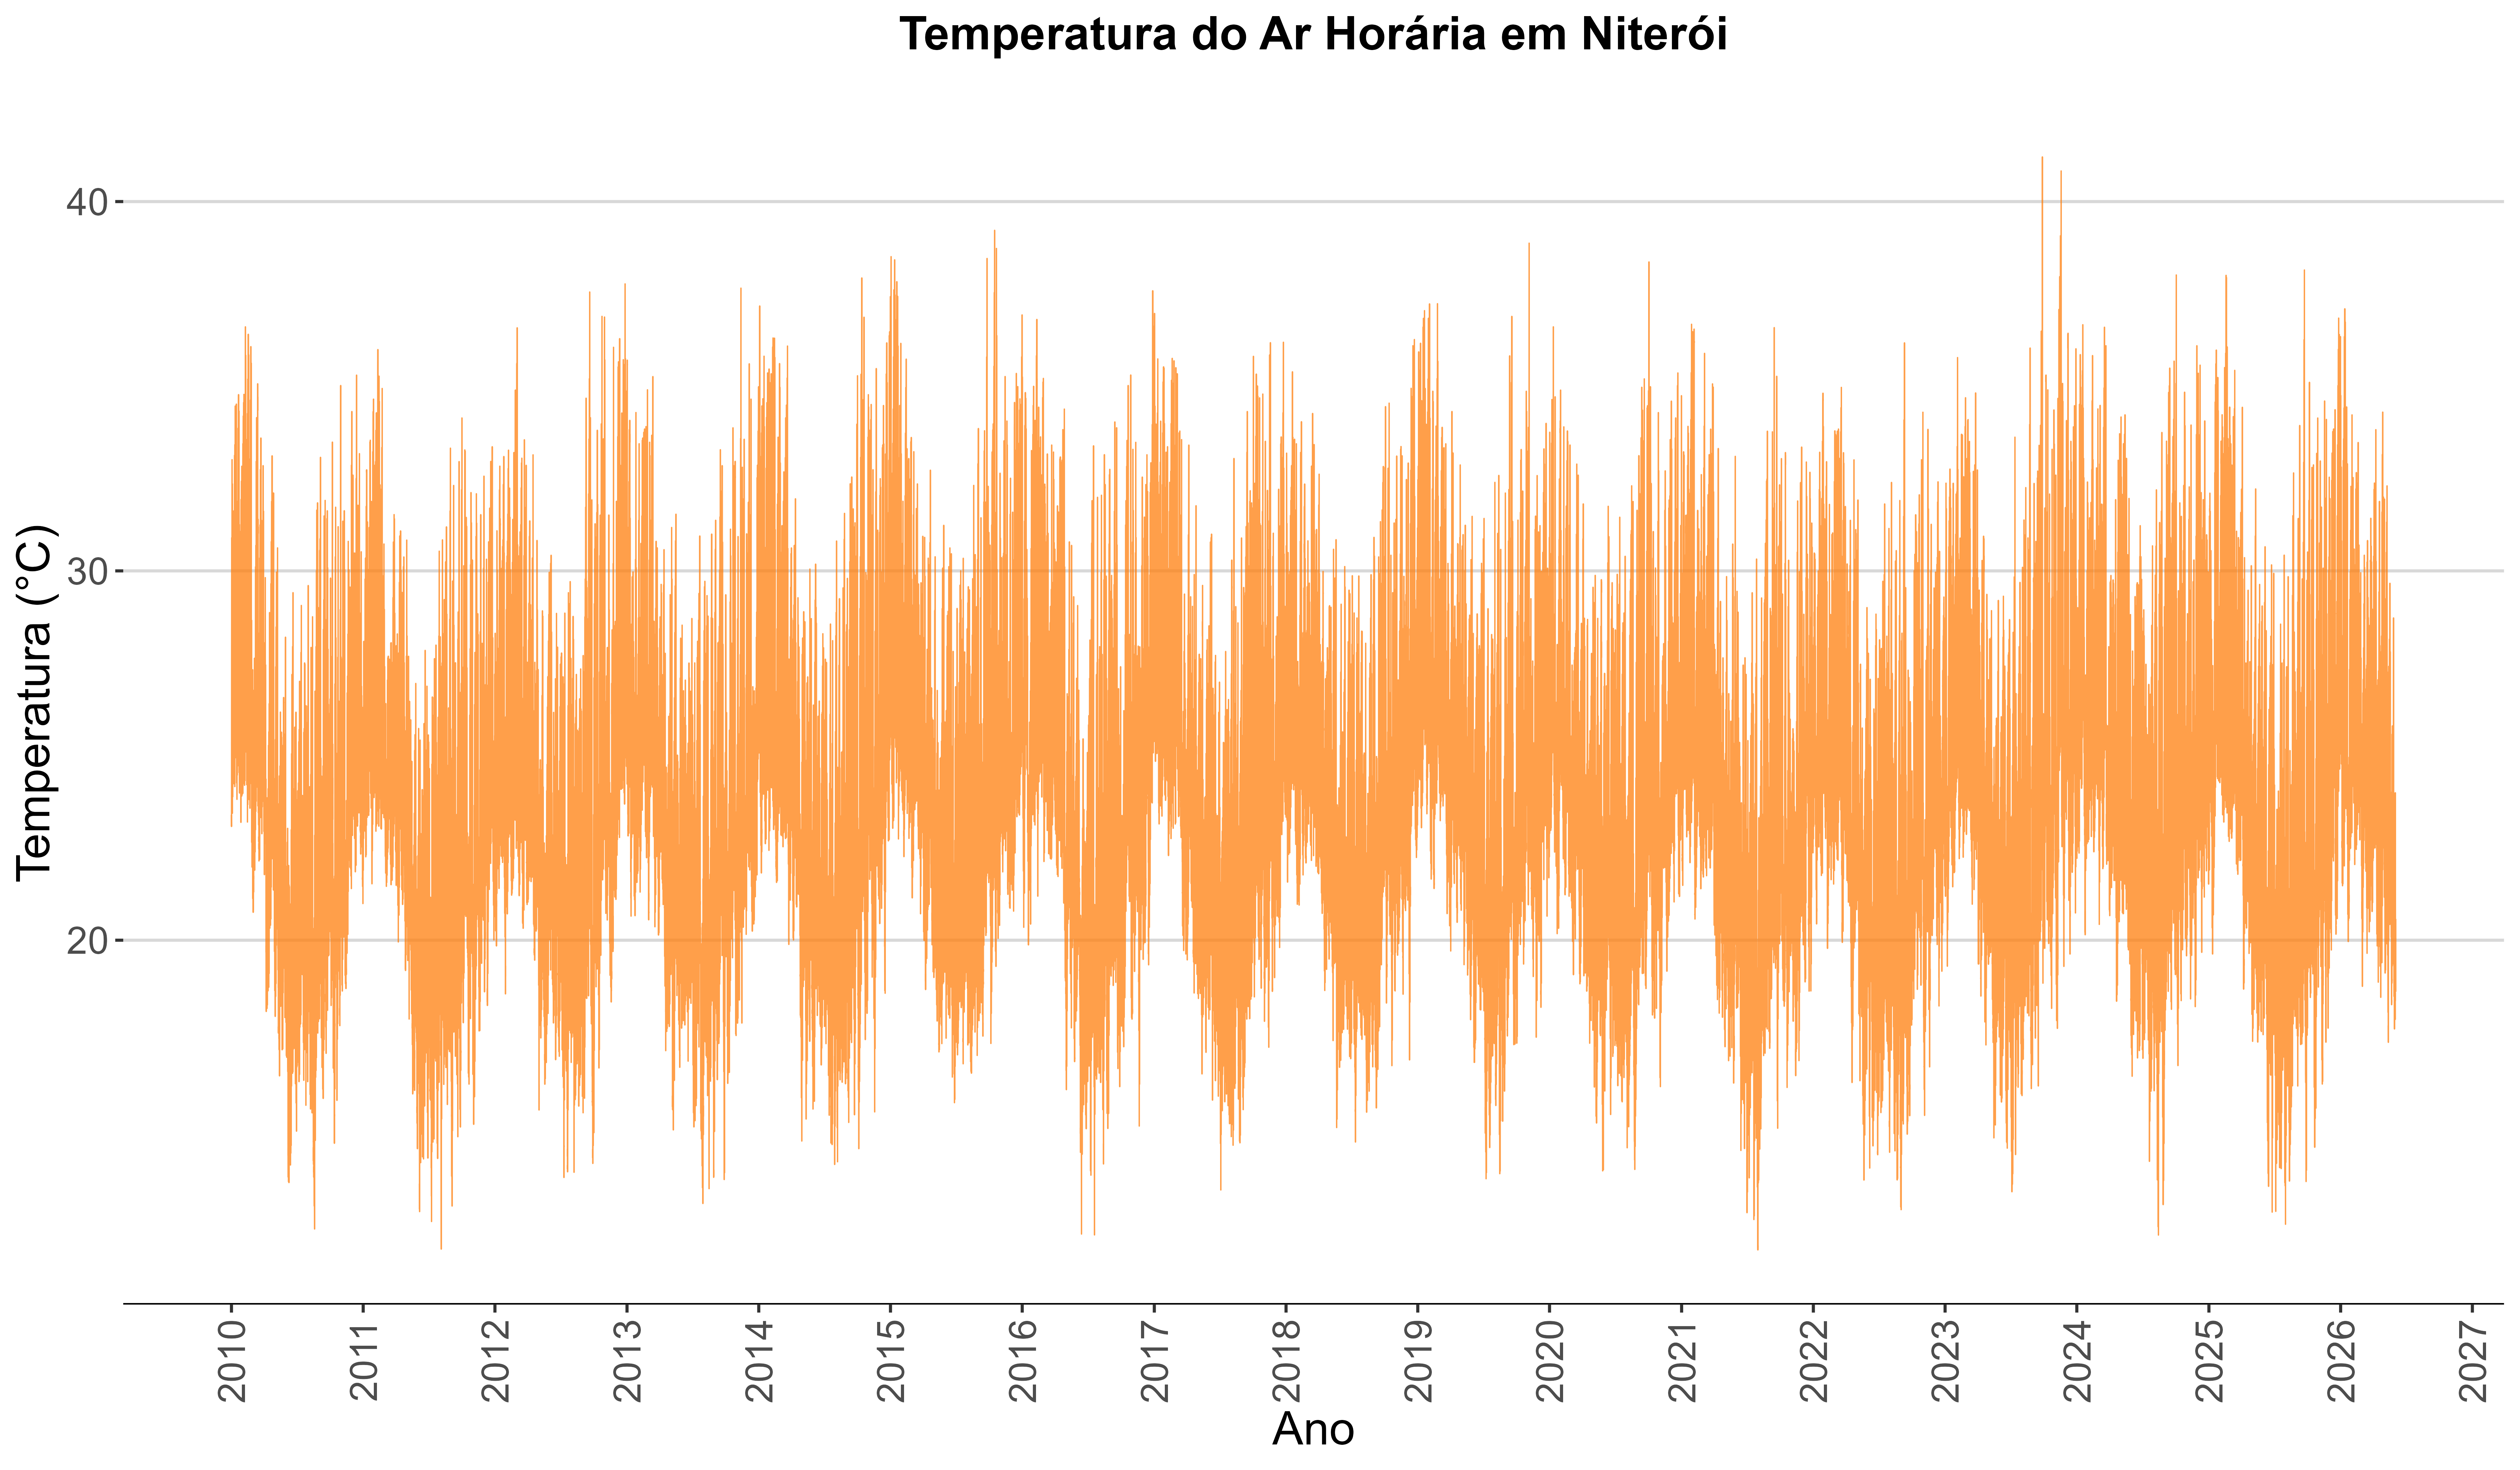
\includegraphics[keepaspectratio]{resultados/Temperatura/00_temperatura_horaria.png}}

}

\caption{Temperatura do Ar Horária}

\end{figure}%

\begin{figure}[H]

{\centering \pandocbounded{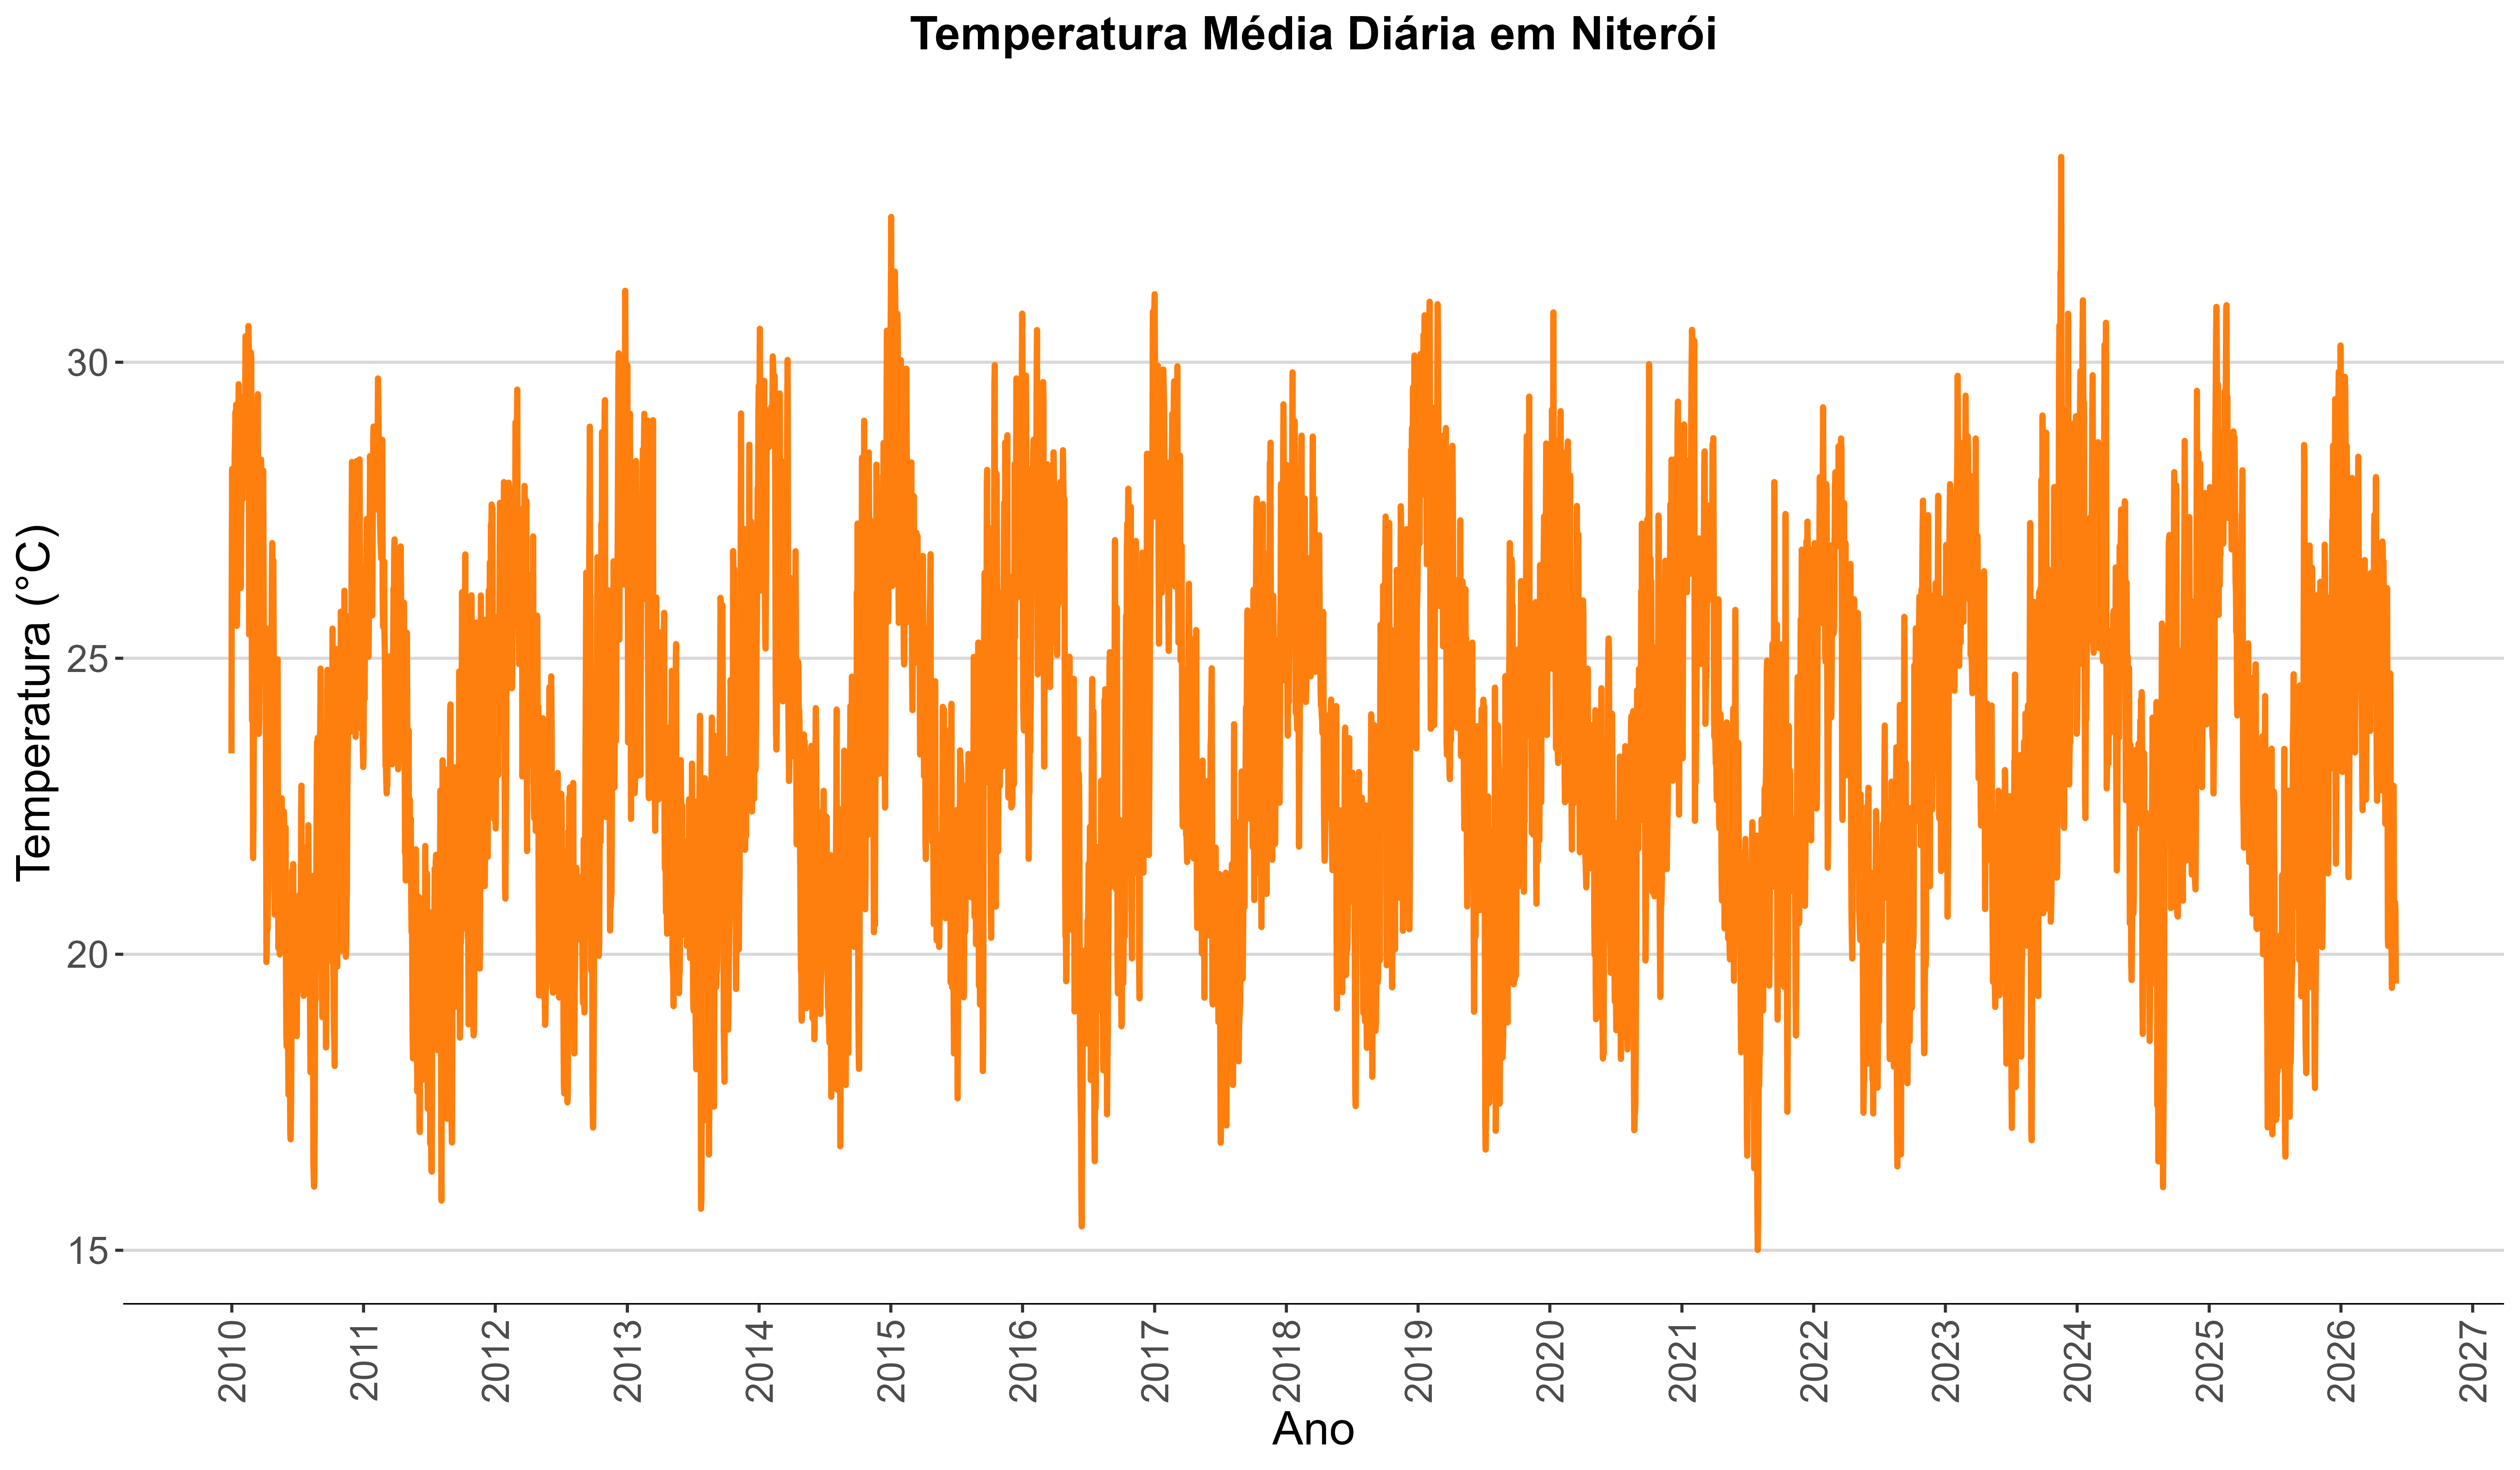
\includegraphics[keepaspectratio]{resultados/Temperatura/01_temperatura_media_diaria.png}}

}

\caption{Temperatura Média Diária}

\end{figure}%

\begin{figure}[H]

{\centering \pandocbounded{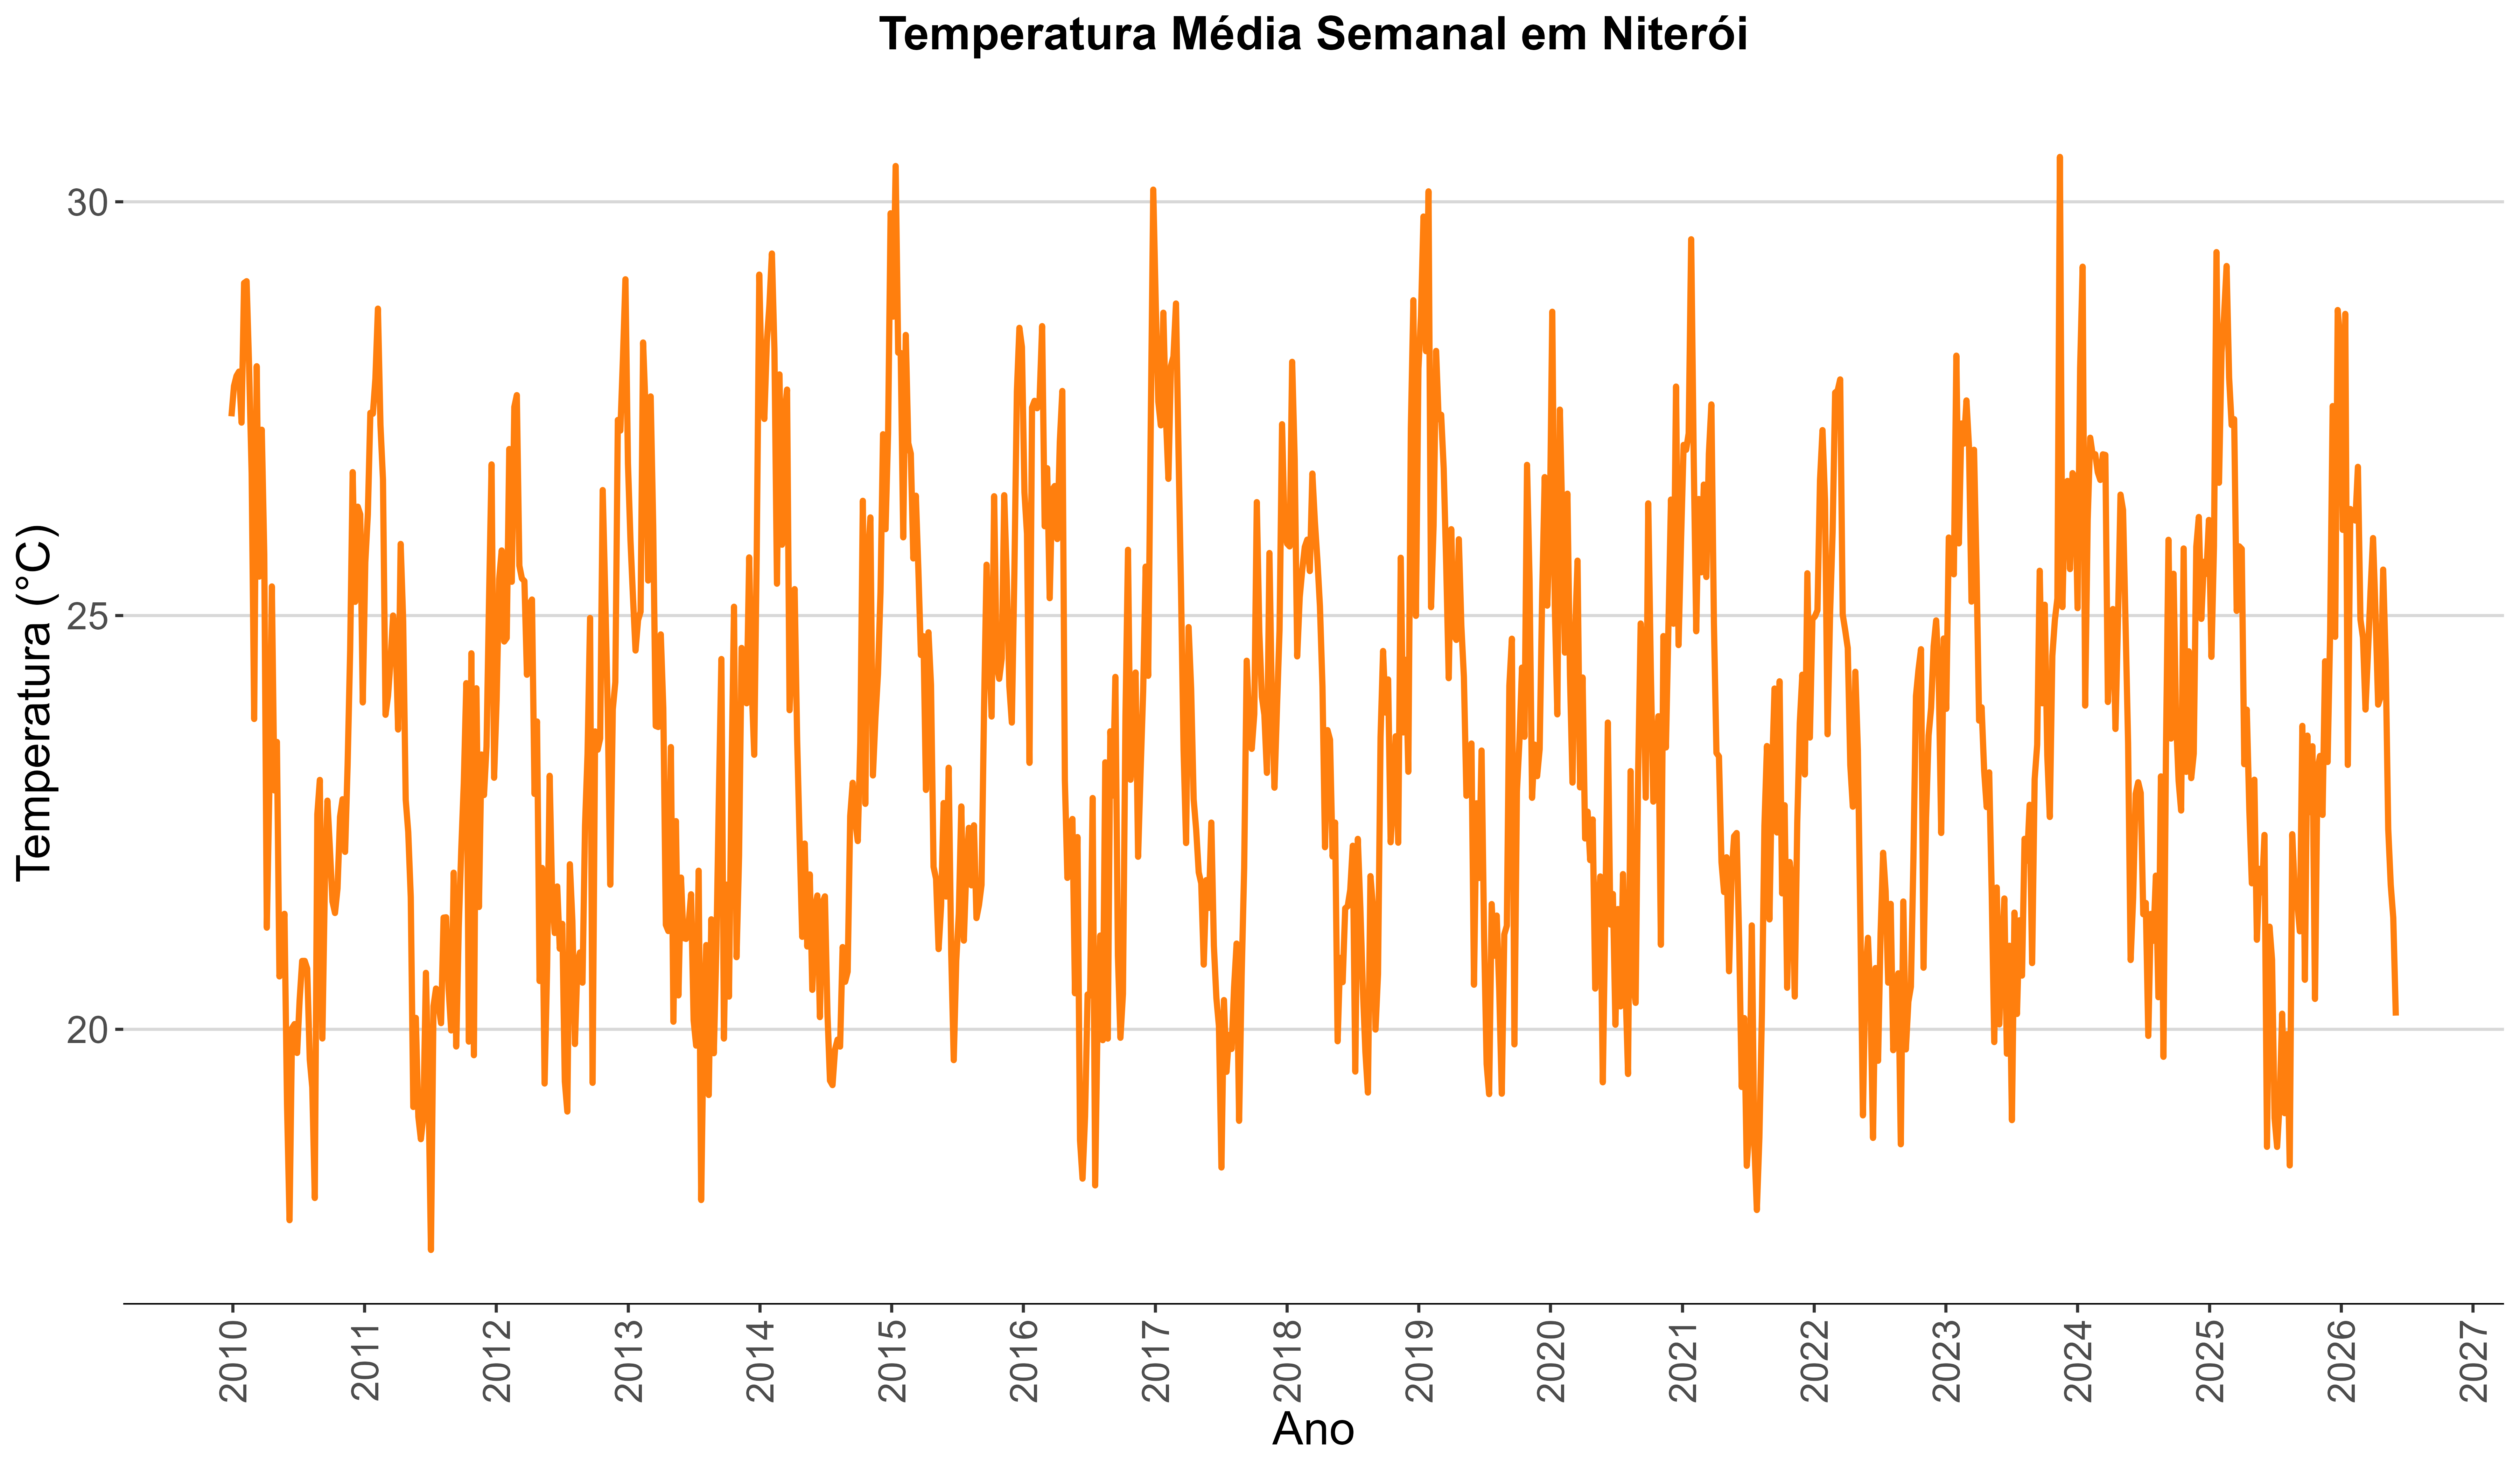
\includegraphics[keepaspectratio]{resultados/Temperatura/02_temperatura_media_semanal.png}}

}

\caption{Temperatura Média Semanal}

\end{figure}%

\begin{figure}[H]

{\centering \pandocbounded{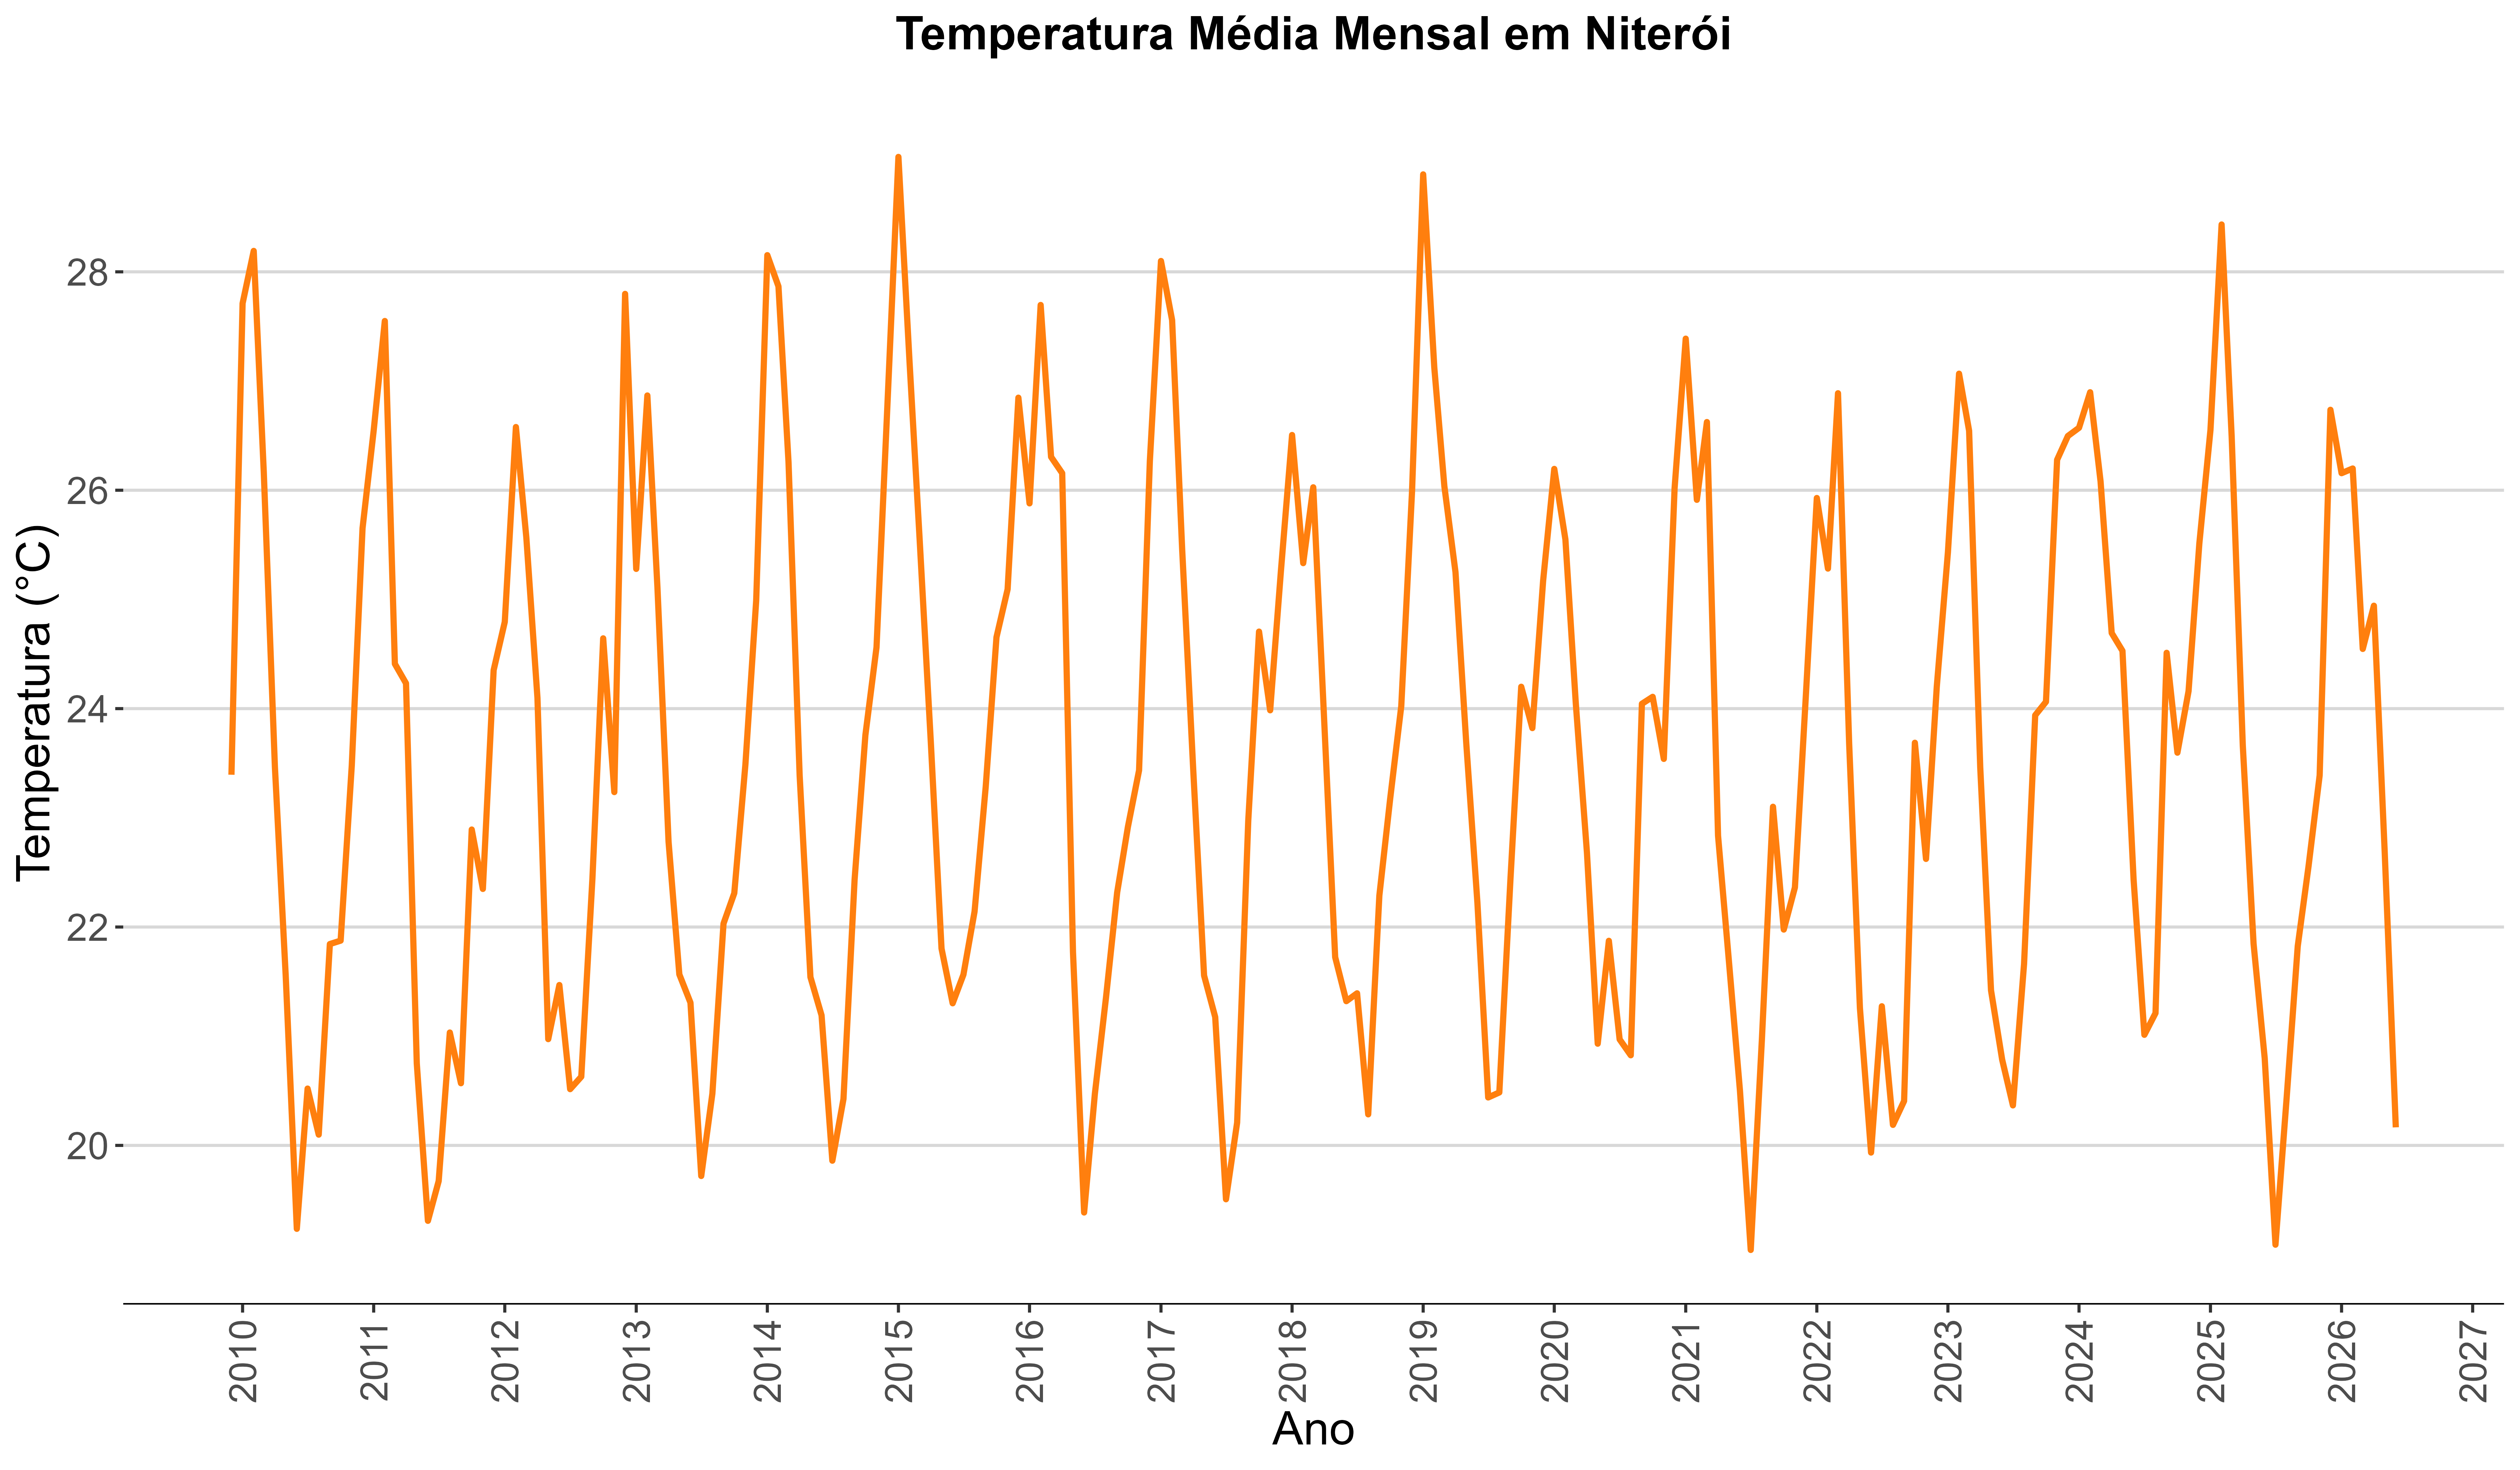
\includegraphics[keepaspectratio]{resultados/Temperatura/03_temperatura_media_mensal.png}}

}

\caption{Temperatura Média Mensal}

\end{figure}%

\begin{figure}[H]

{\centering \pandocbounded{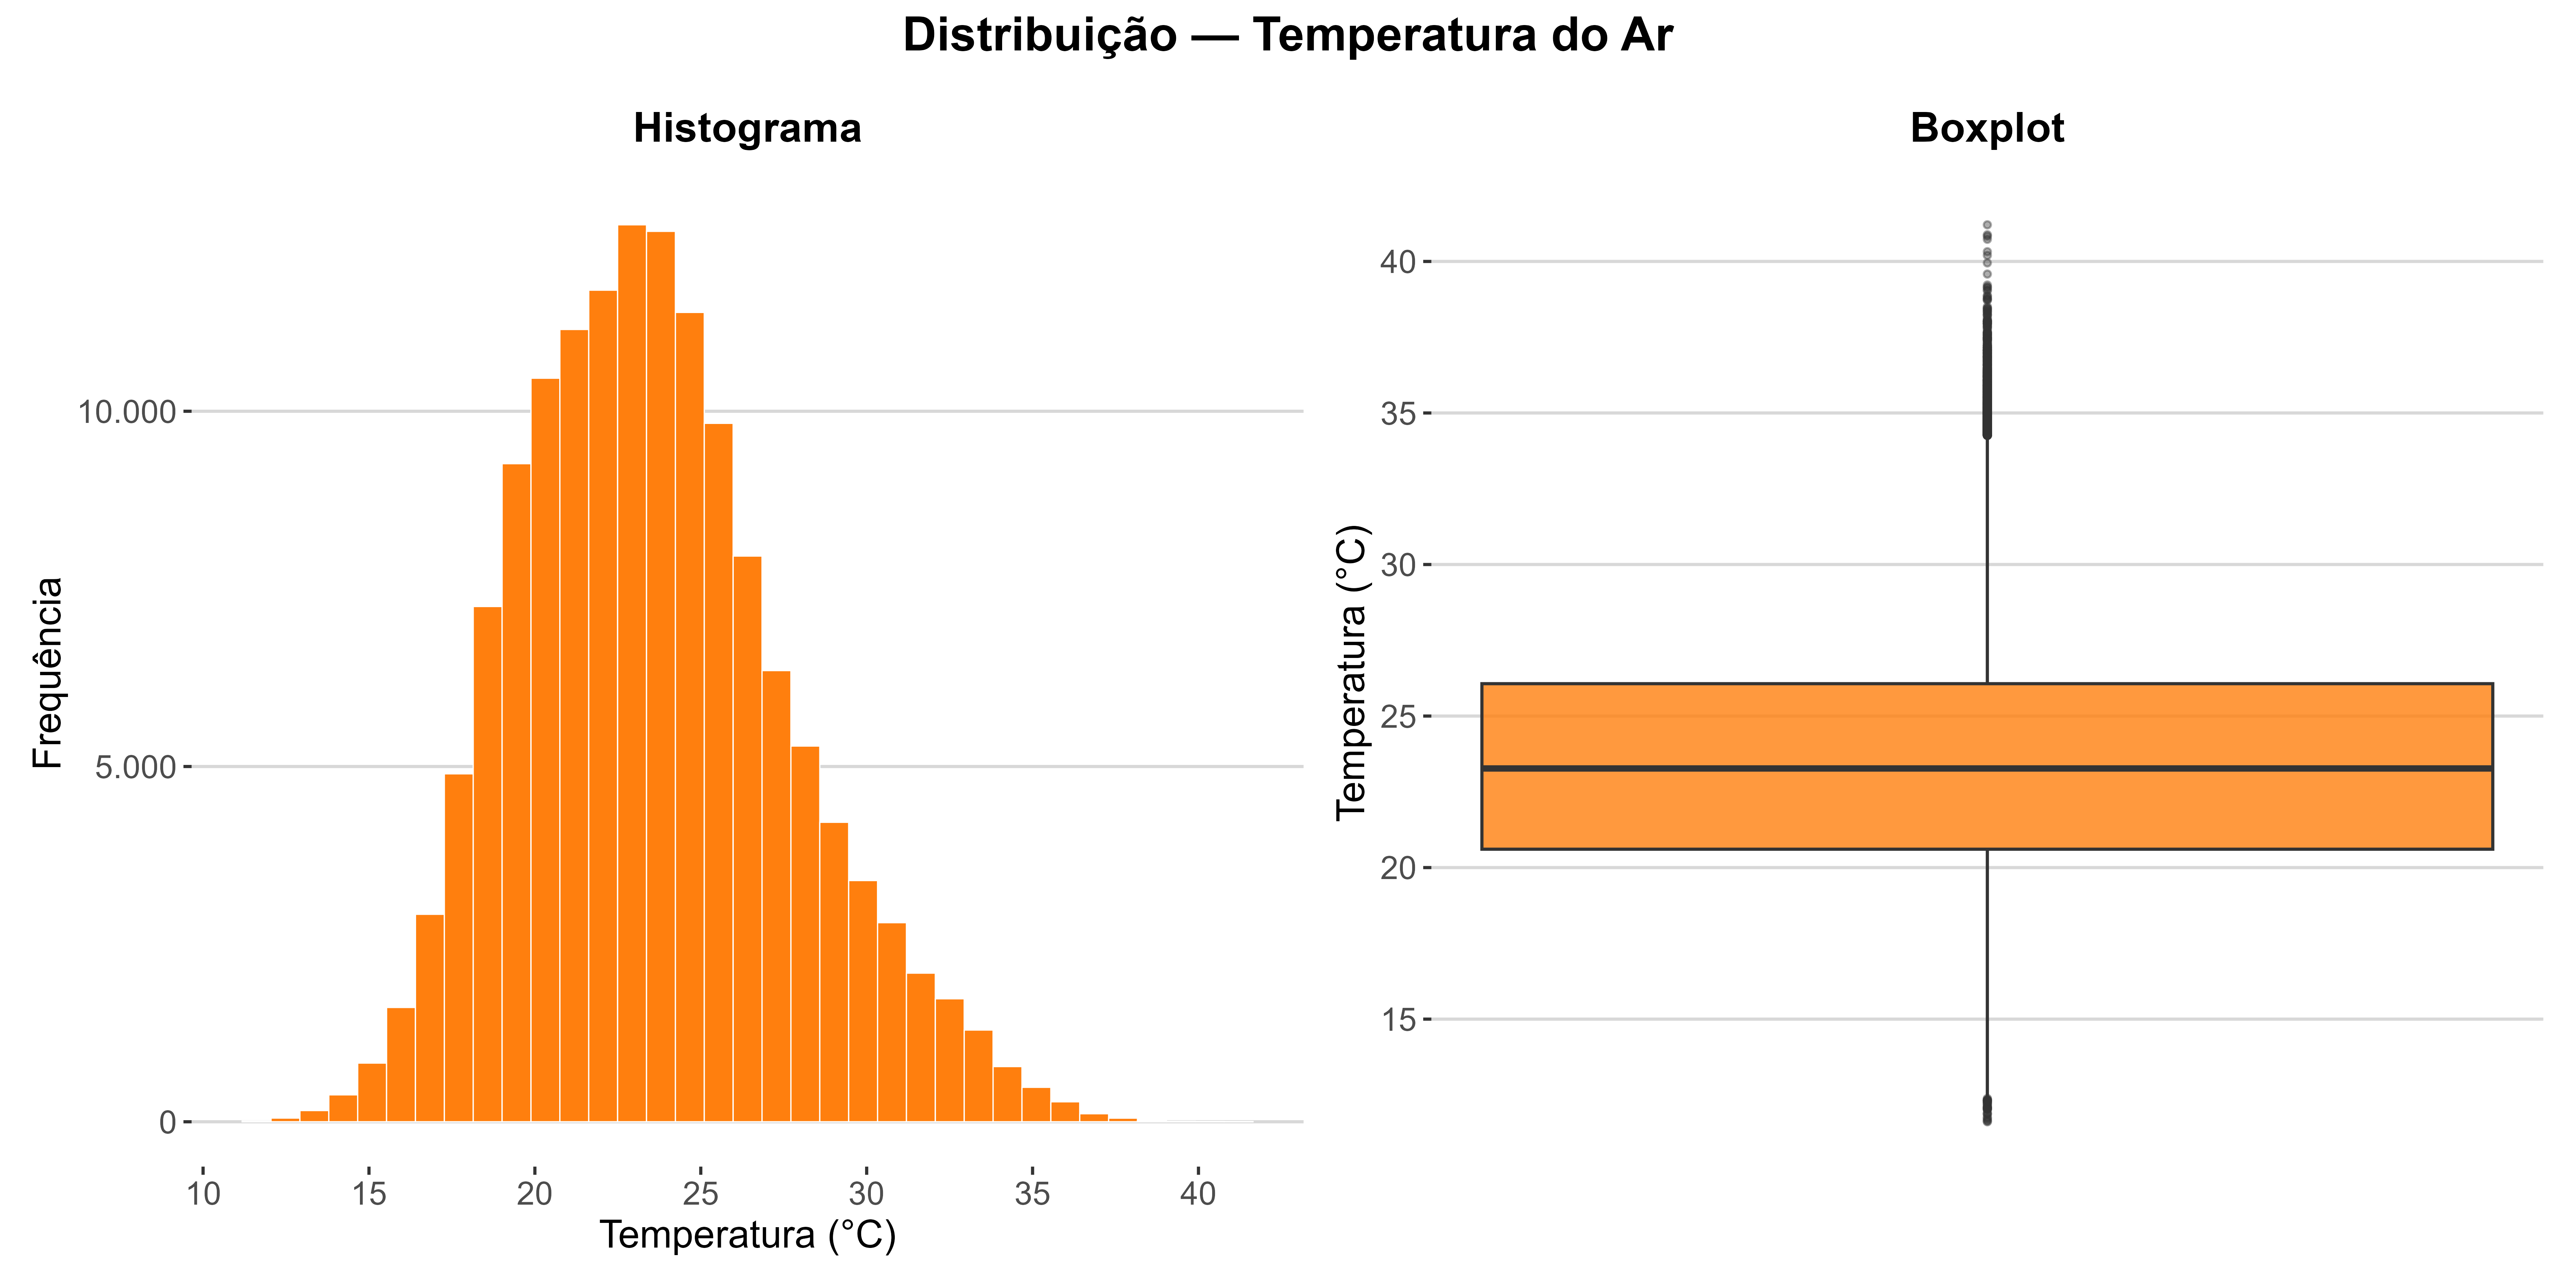
\includegraphics[keepaspectratio]{resultados/Temperatura/04_temperatura_distribuicao.png}}

}

\caption{Distribuição da Temperatura}

\end{figure}%

\subsubsection{Principais Achados}\label{principais-achados}

As séries horárias e diárias revelam uma \textbf{sazonalidade anual
muito pronunciada}: picos de temperatura (próximos a 40 °C) ocorrem
sistematicamente no verão (dezembro--fevereiro), enquanto os valores
mínimos (abaixo de 15 °C) concentram-se no inverno (junho--agosto).

Na escala horária, a amplitude diária é elevada --- chegando a 15--20 °C
entre a madrugada e a tarde ---, o que reforça a importância de uma
janela de entrada suficientemente longa para o modelo LSTM.

Na escala mensal, a temperatura média oscila entre aproximadamente 20 °C
(inverno) e 28 °C (verão), sem tendência de aquecimento visível ao longo
dos 17 anos da série.

O histograma mostra distribuição \textbf{ligeiramente assimétrica à
direita}, com moda em torno de 24--25 °C e cauda superior estendida até
\textasciitilde40 °C. O boxplot confirma a ausência de outliers extremos
inferiores, mas evidencia alguns pontos acima de 38 °C, provavelmente
associados a ondas de calor no verão.

\subsection{Covariáveis}\label{covariuxe1veis}

\subsubsection{Umidade Relativa}\label{umidade-relativa}

\begin{figure}[H]

{\centering \pandocbounded{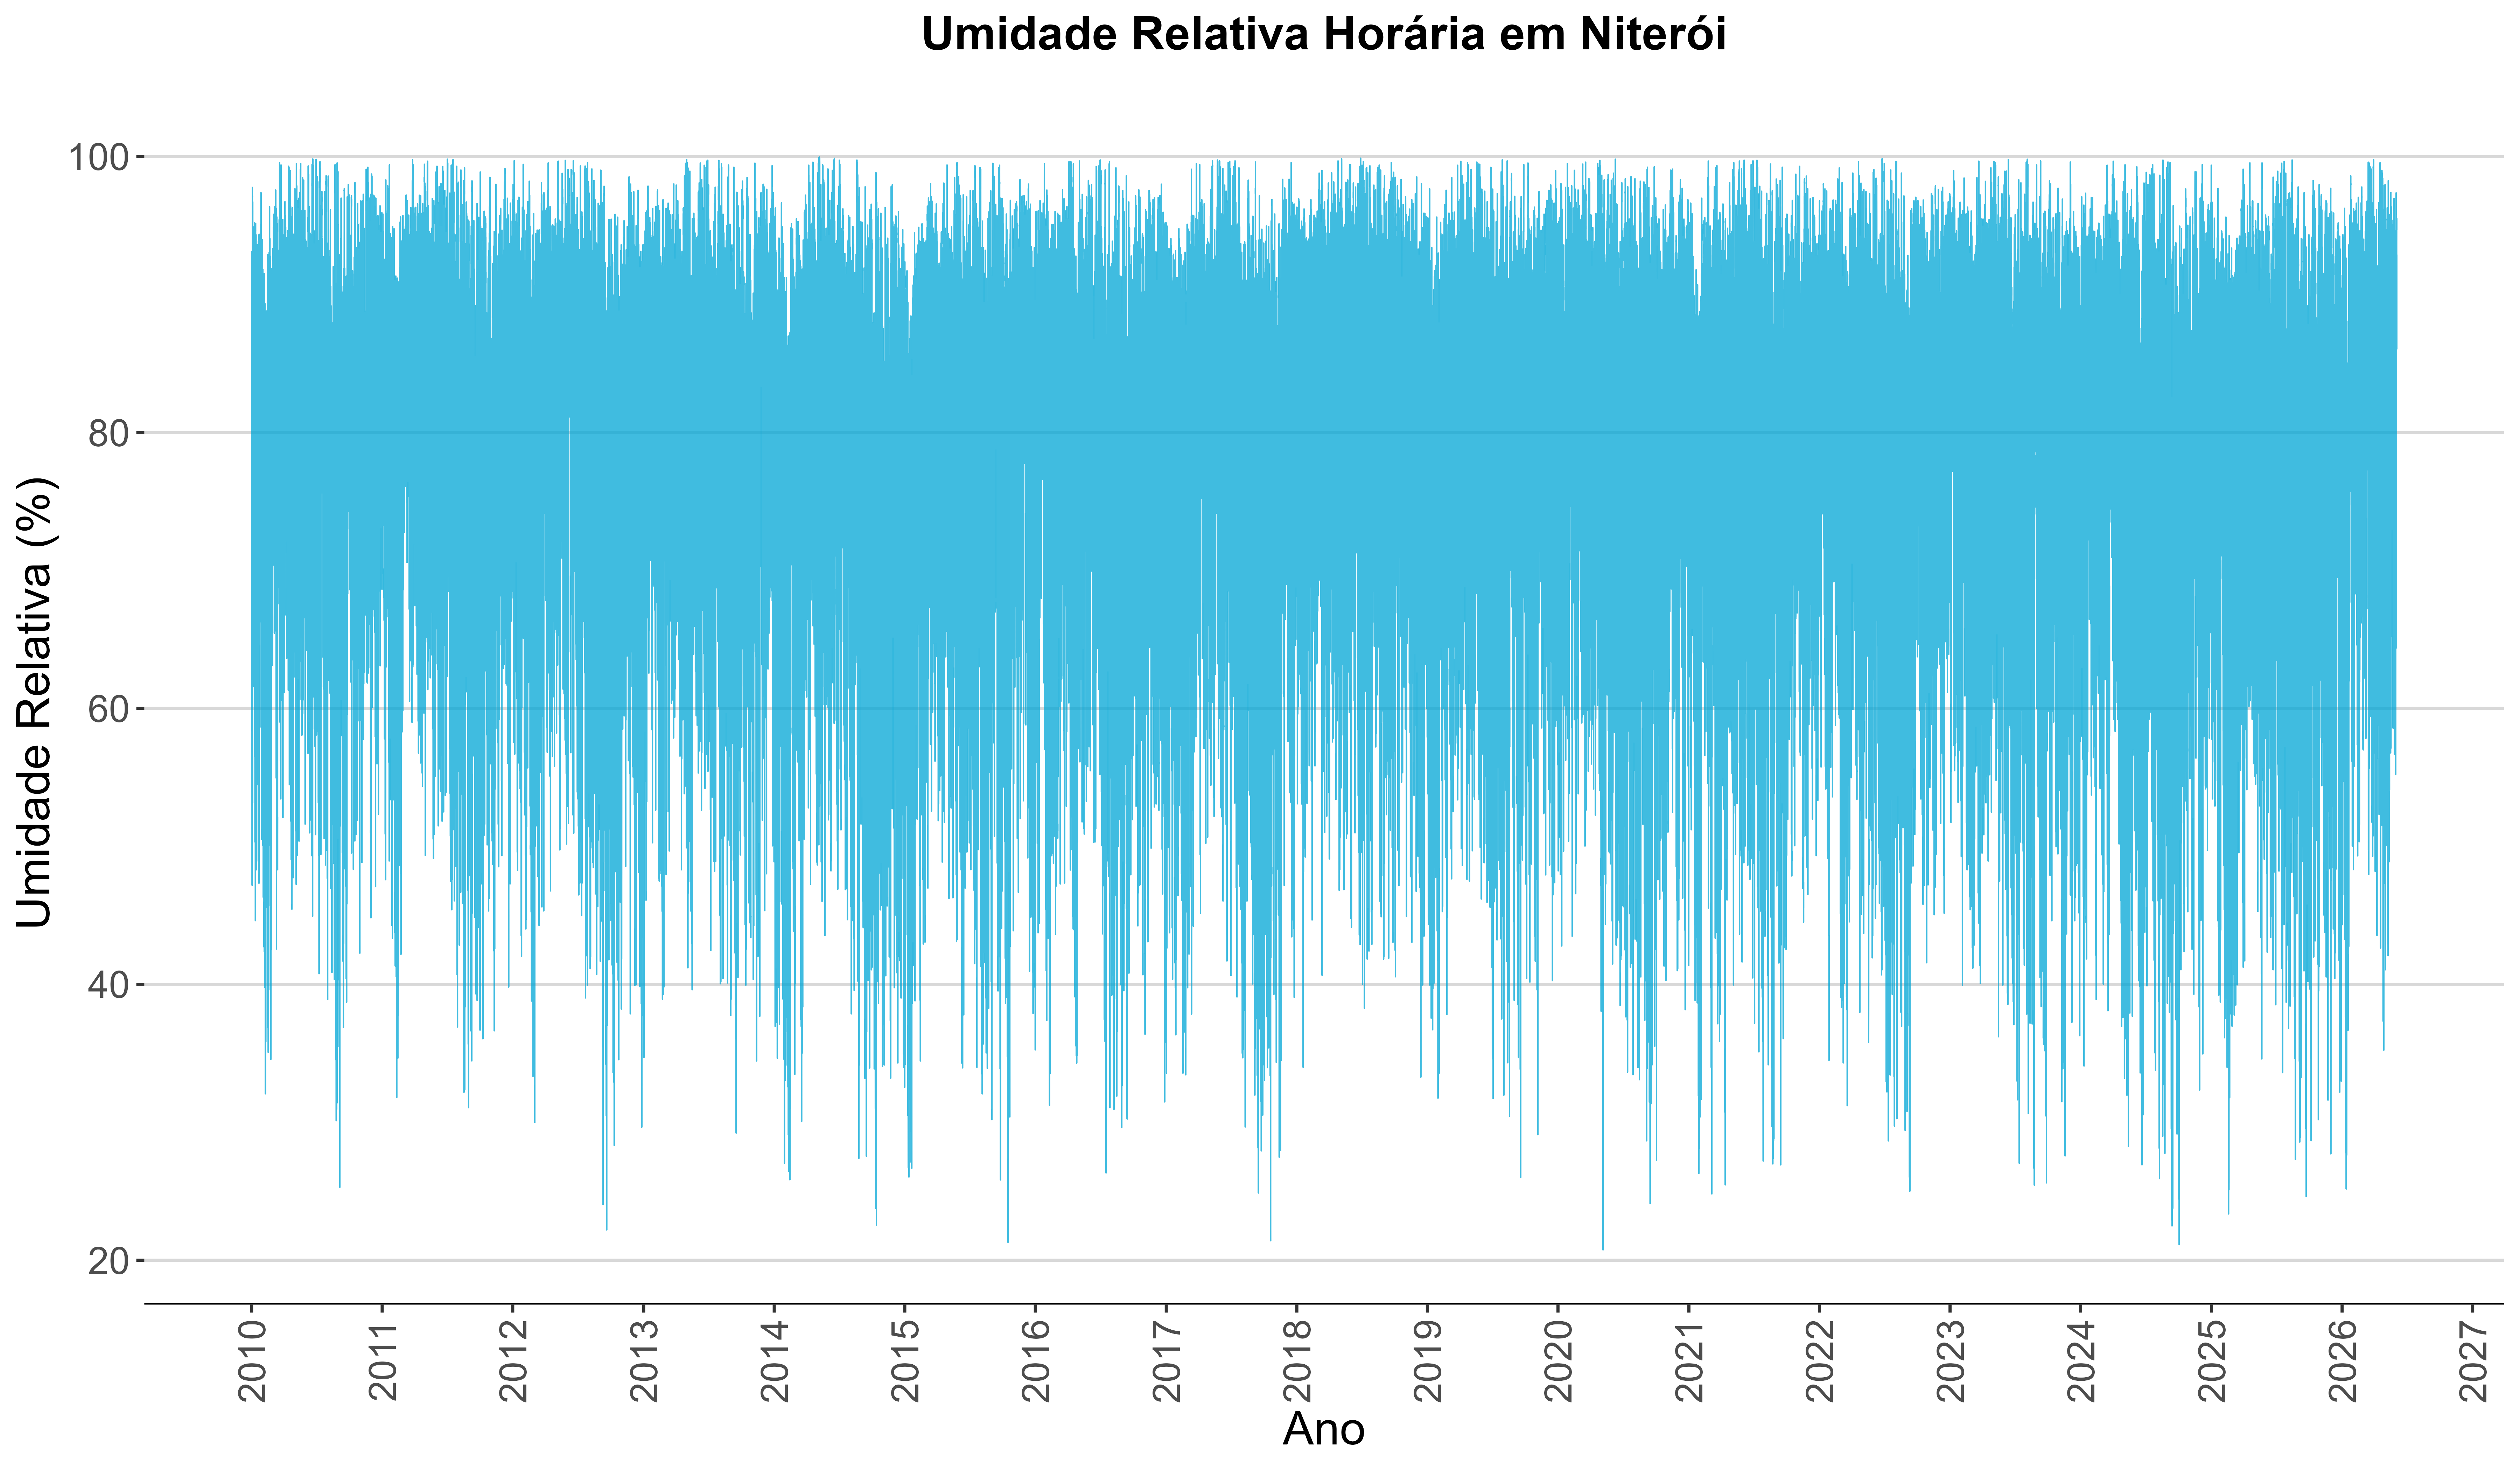
\includegraphics[keepaspectratio]{resultados/UmidadRel/00_umidade_relativa_horaria.png}}

}

\caption{Umidade Relativa Horária}

\end{figure}%

\begin{figure}[H]

{\centering \pandocbounded{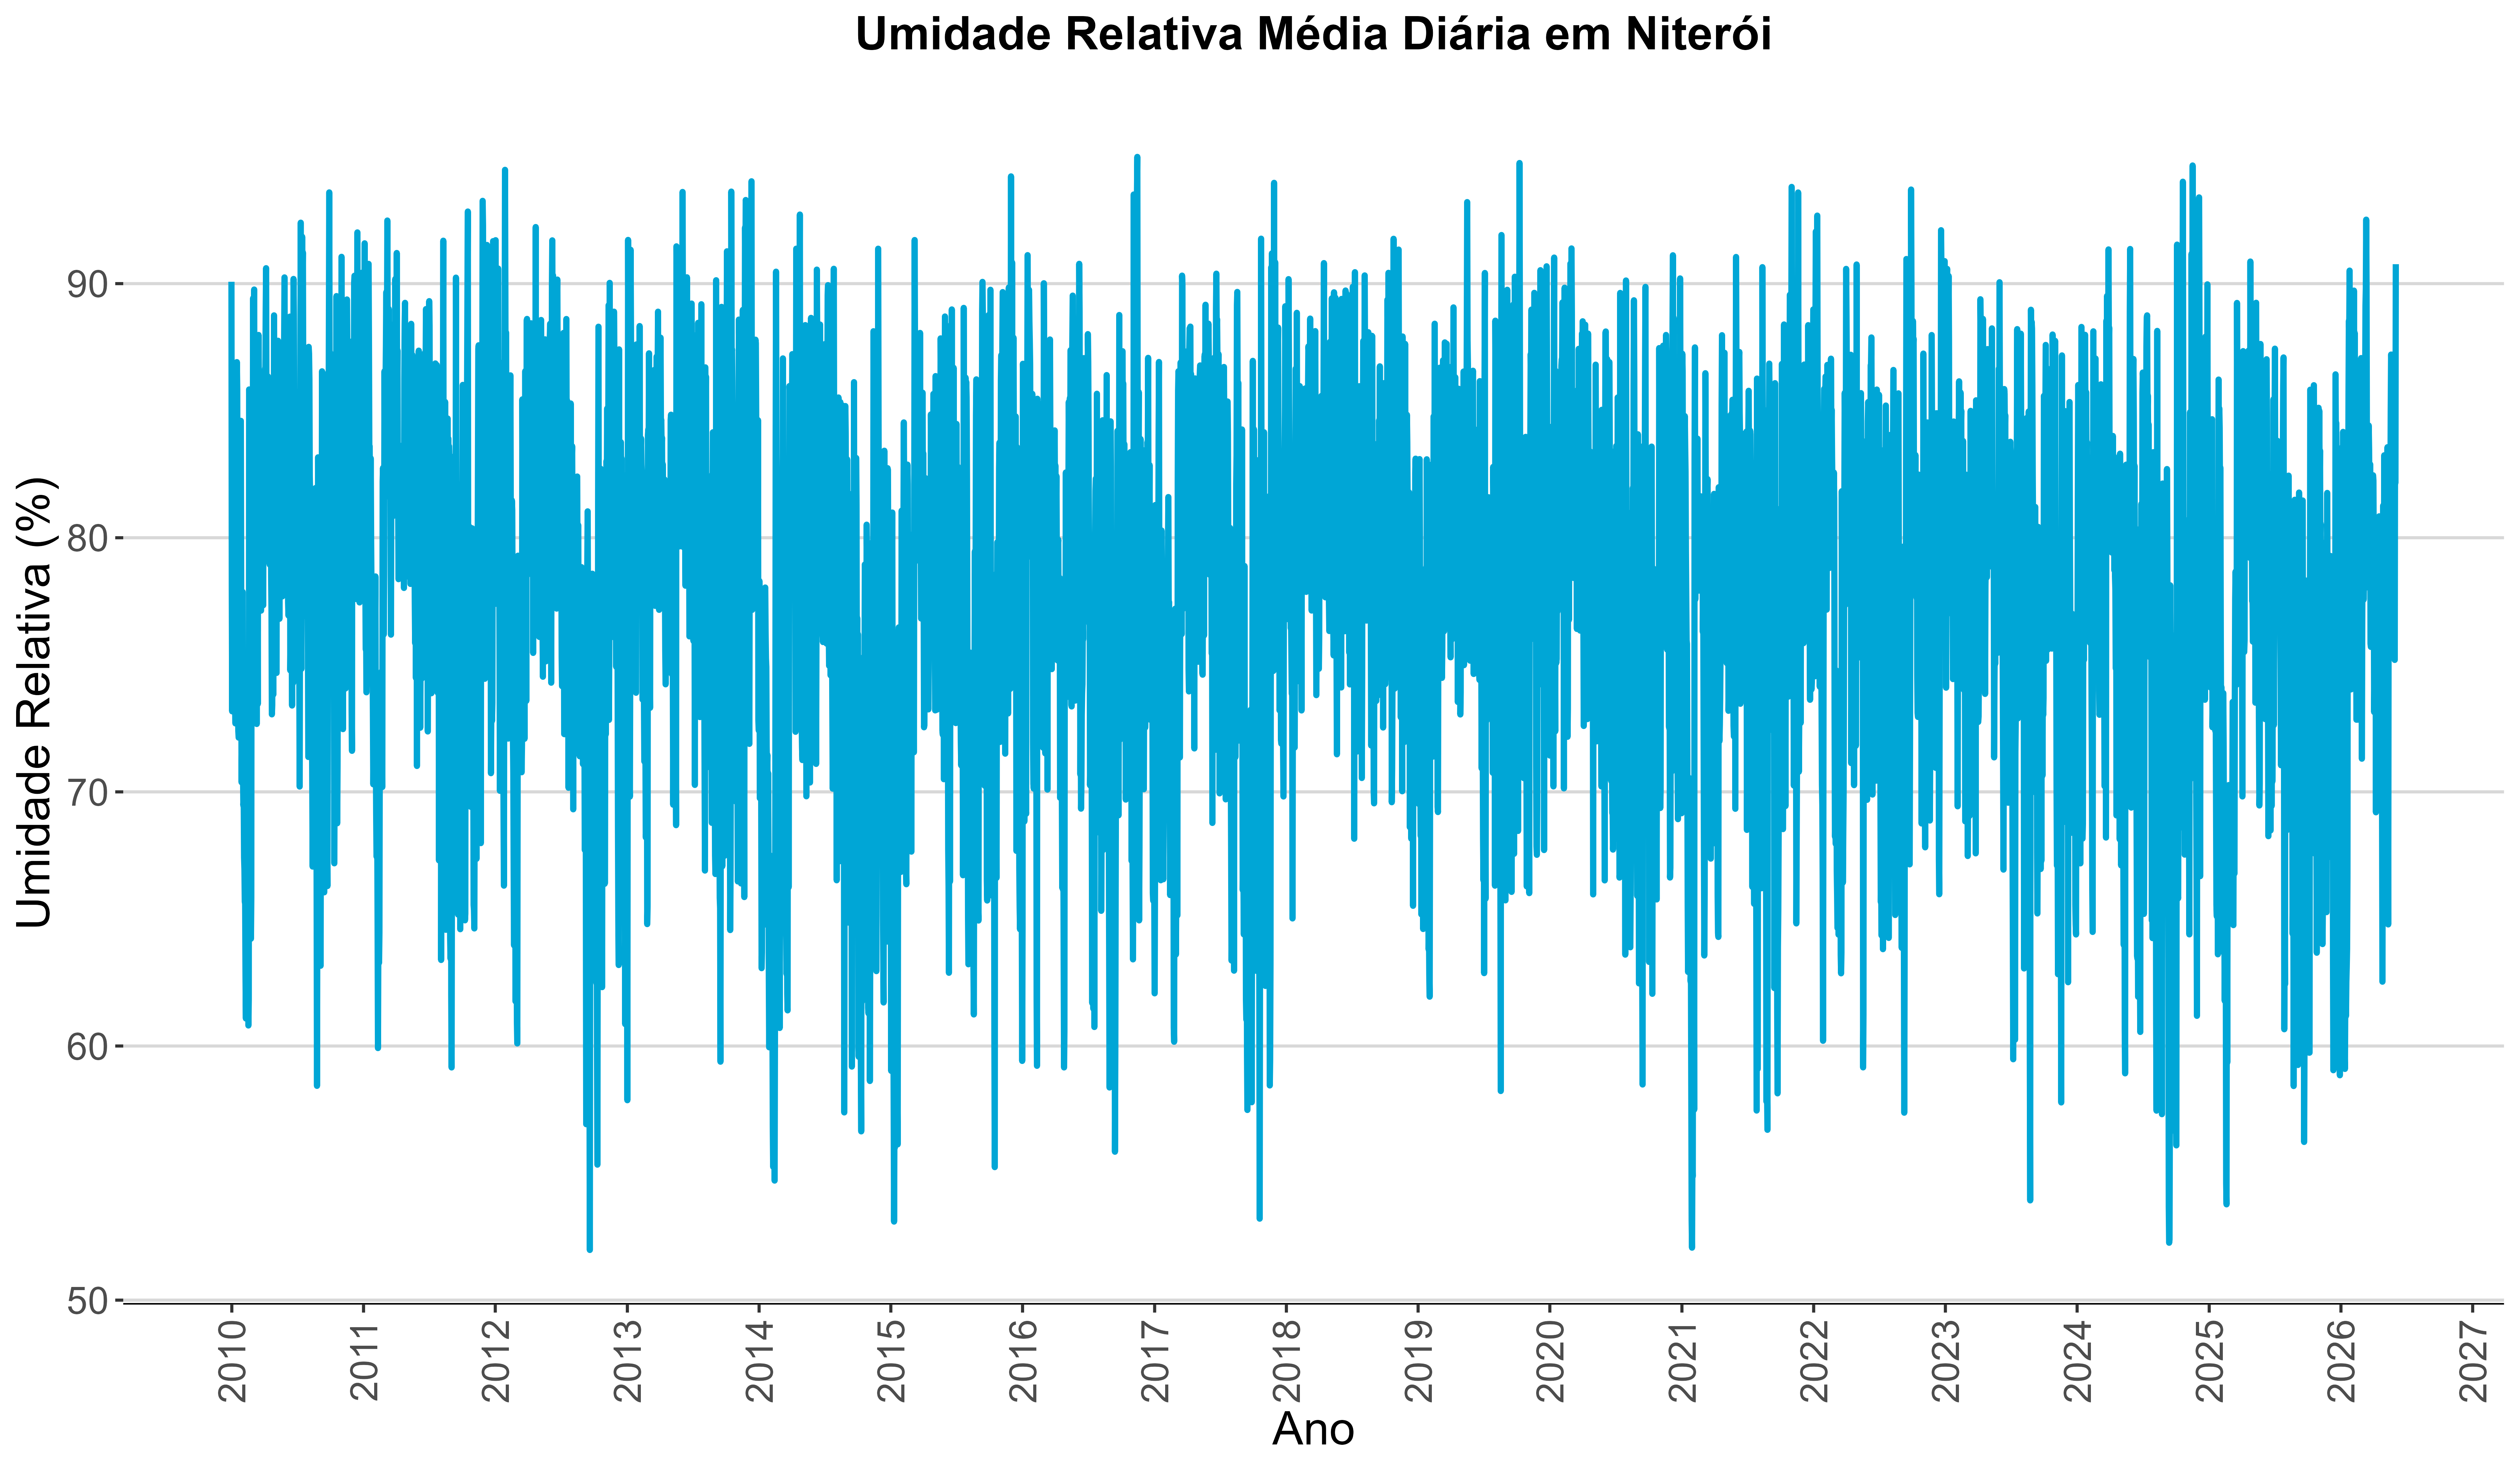
\includegraphics[keepaspectratio]{resultados/UmidadRel/01_umidade_relativa_media_diaria.png}}

}

\caption{Umidade Relativa Média Diária}

\end{figure}%

\begin{figure}[H]

{\centering \pandocbounded{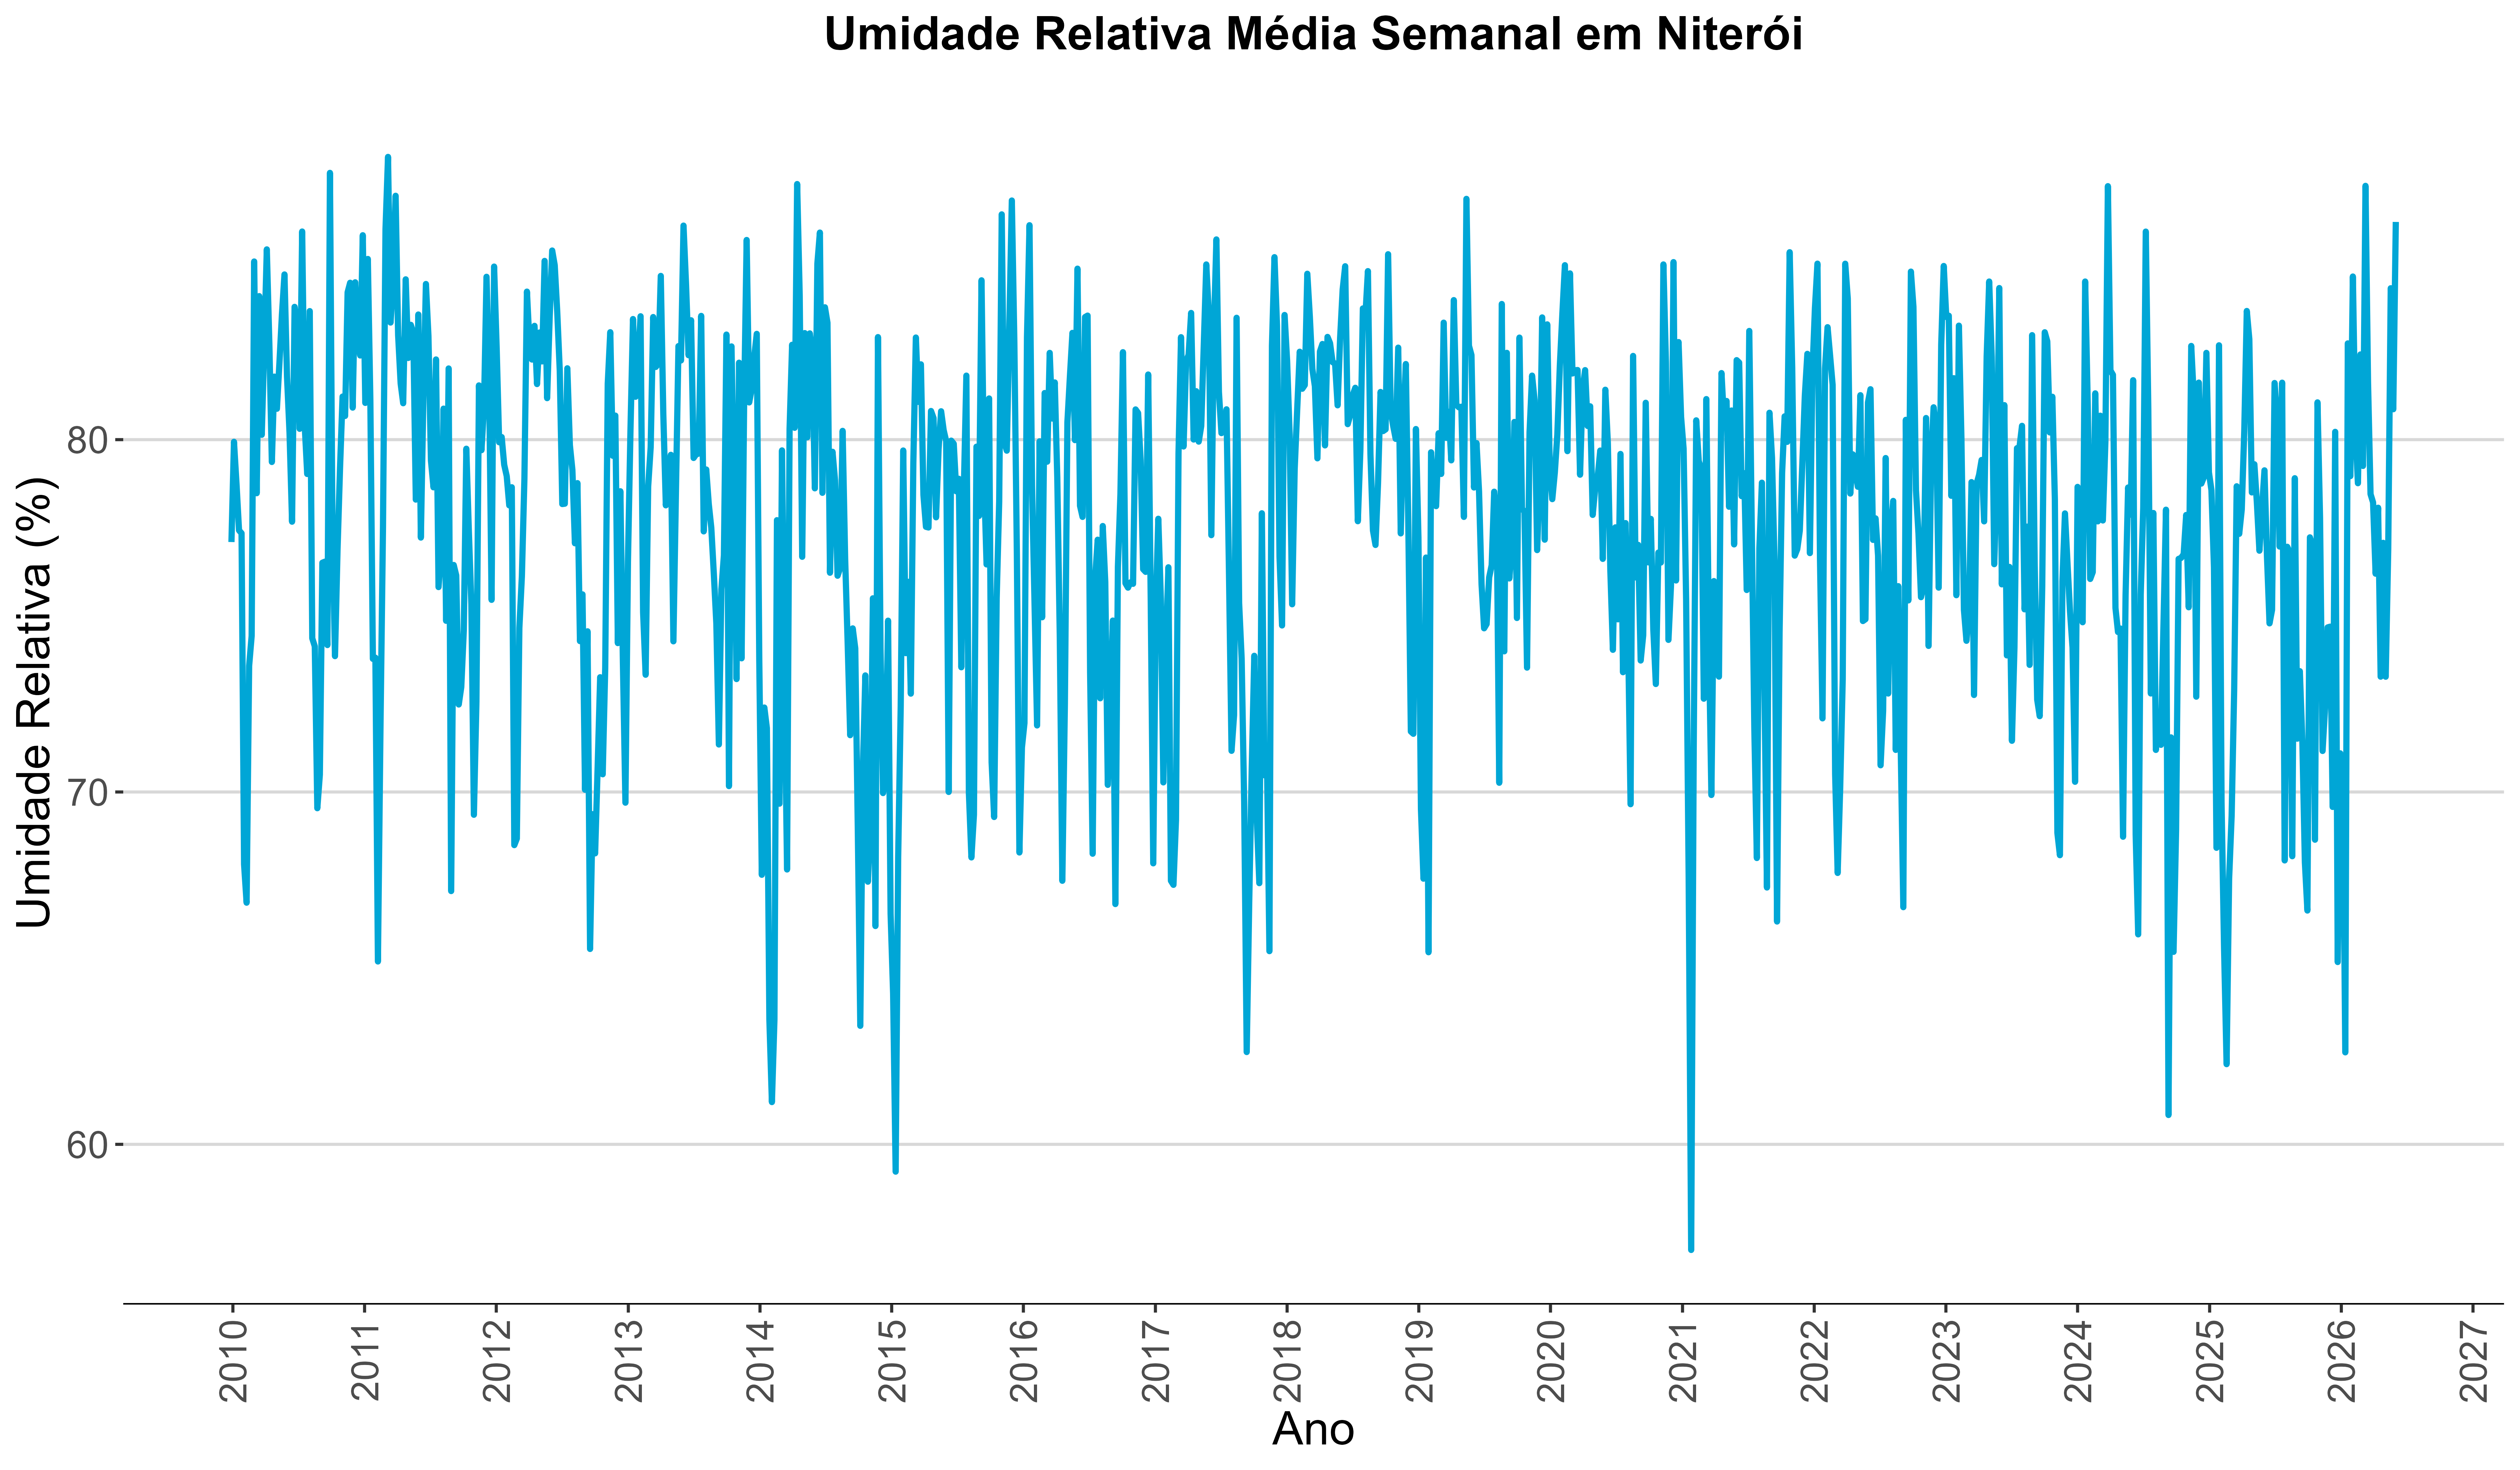
\includegraphics[keepaspectratio]{resultados/UmidadRel/02_umidade_relativa_media_semanal.png}}

}

\caption{Umidade Relativa Média Semanal}

\end{figure}%

\begin{figure}[H]

{\centering \pandocbounded{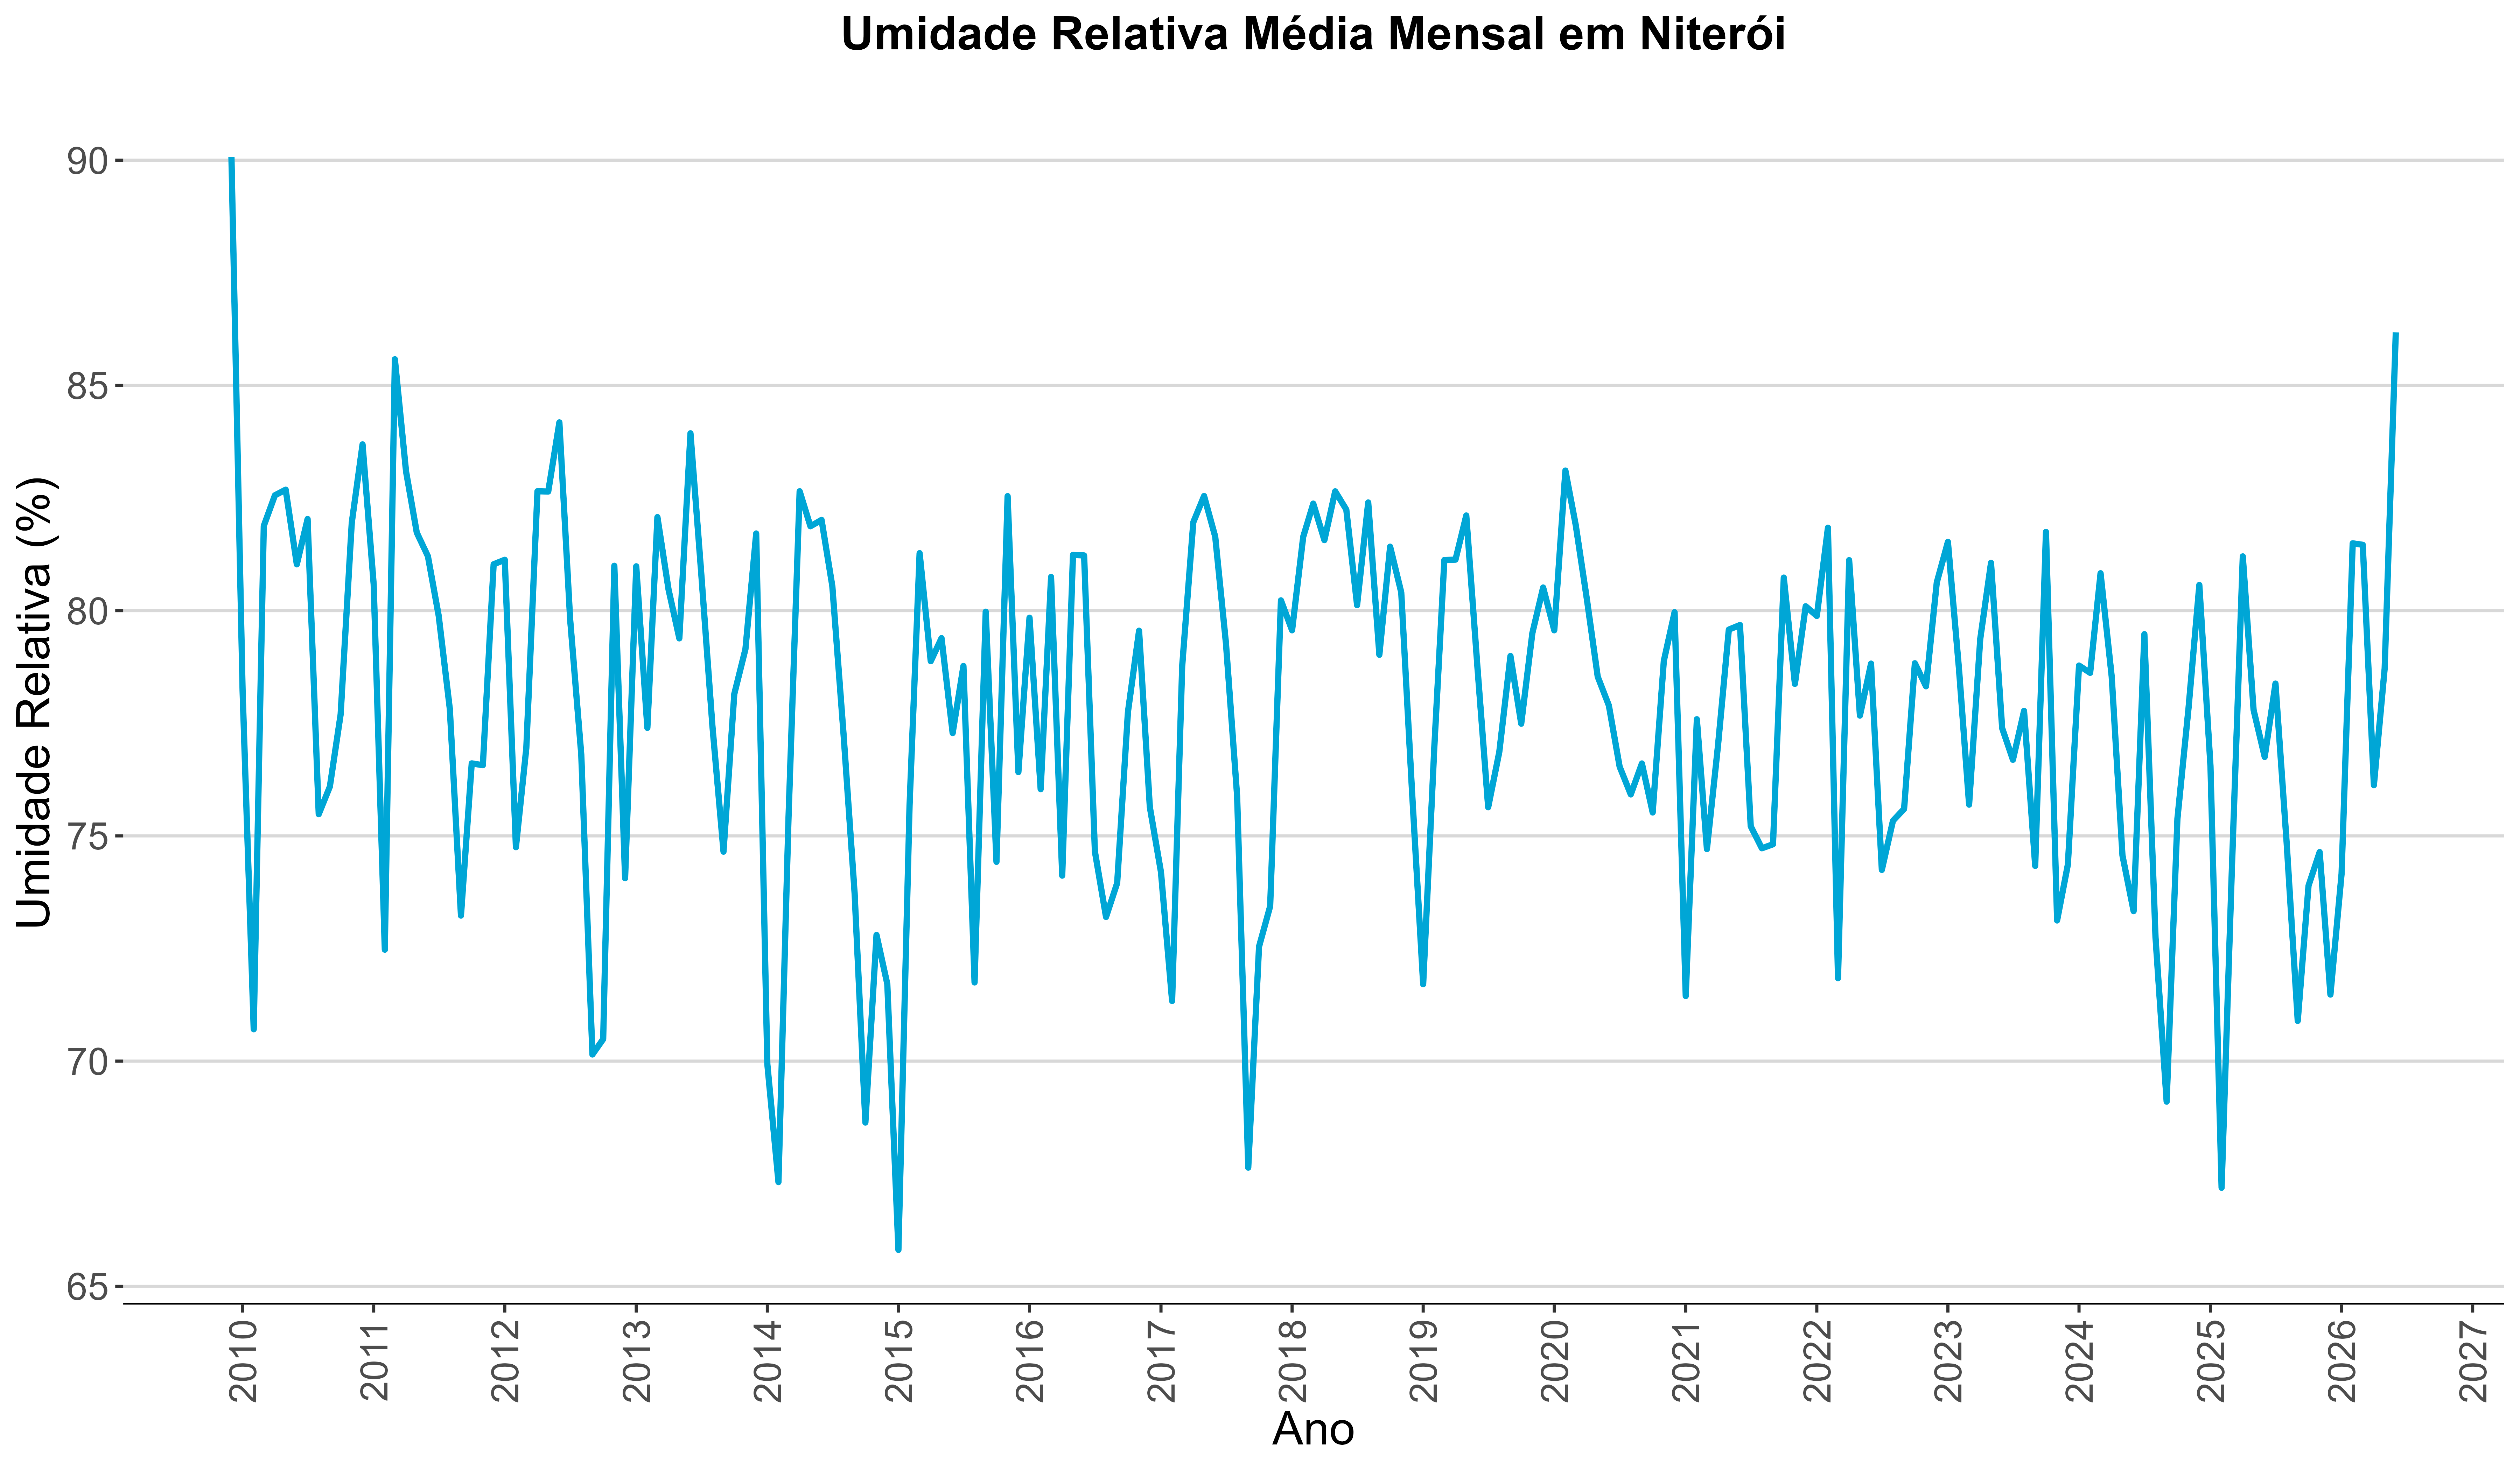
\includegraphics[keepaspectratio]{resultados/UmidadRel/03_umidade_relativa_media_mensal.png}}

}

\caption{Umidade Relativa Média Mensal}

\end{figure}%

\begin{figure}[H]

{\centering \pandocbounded{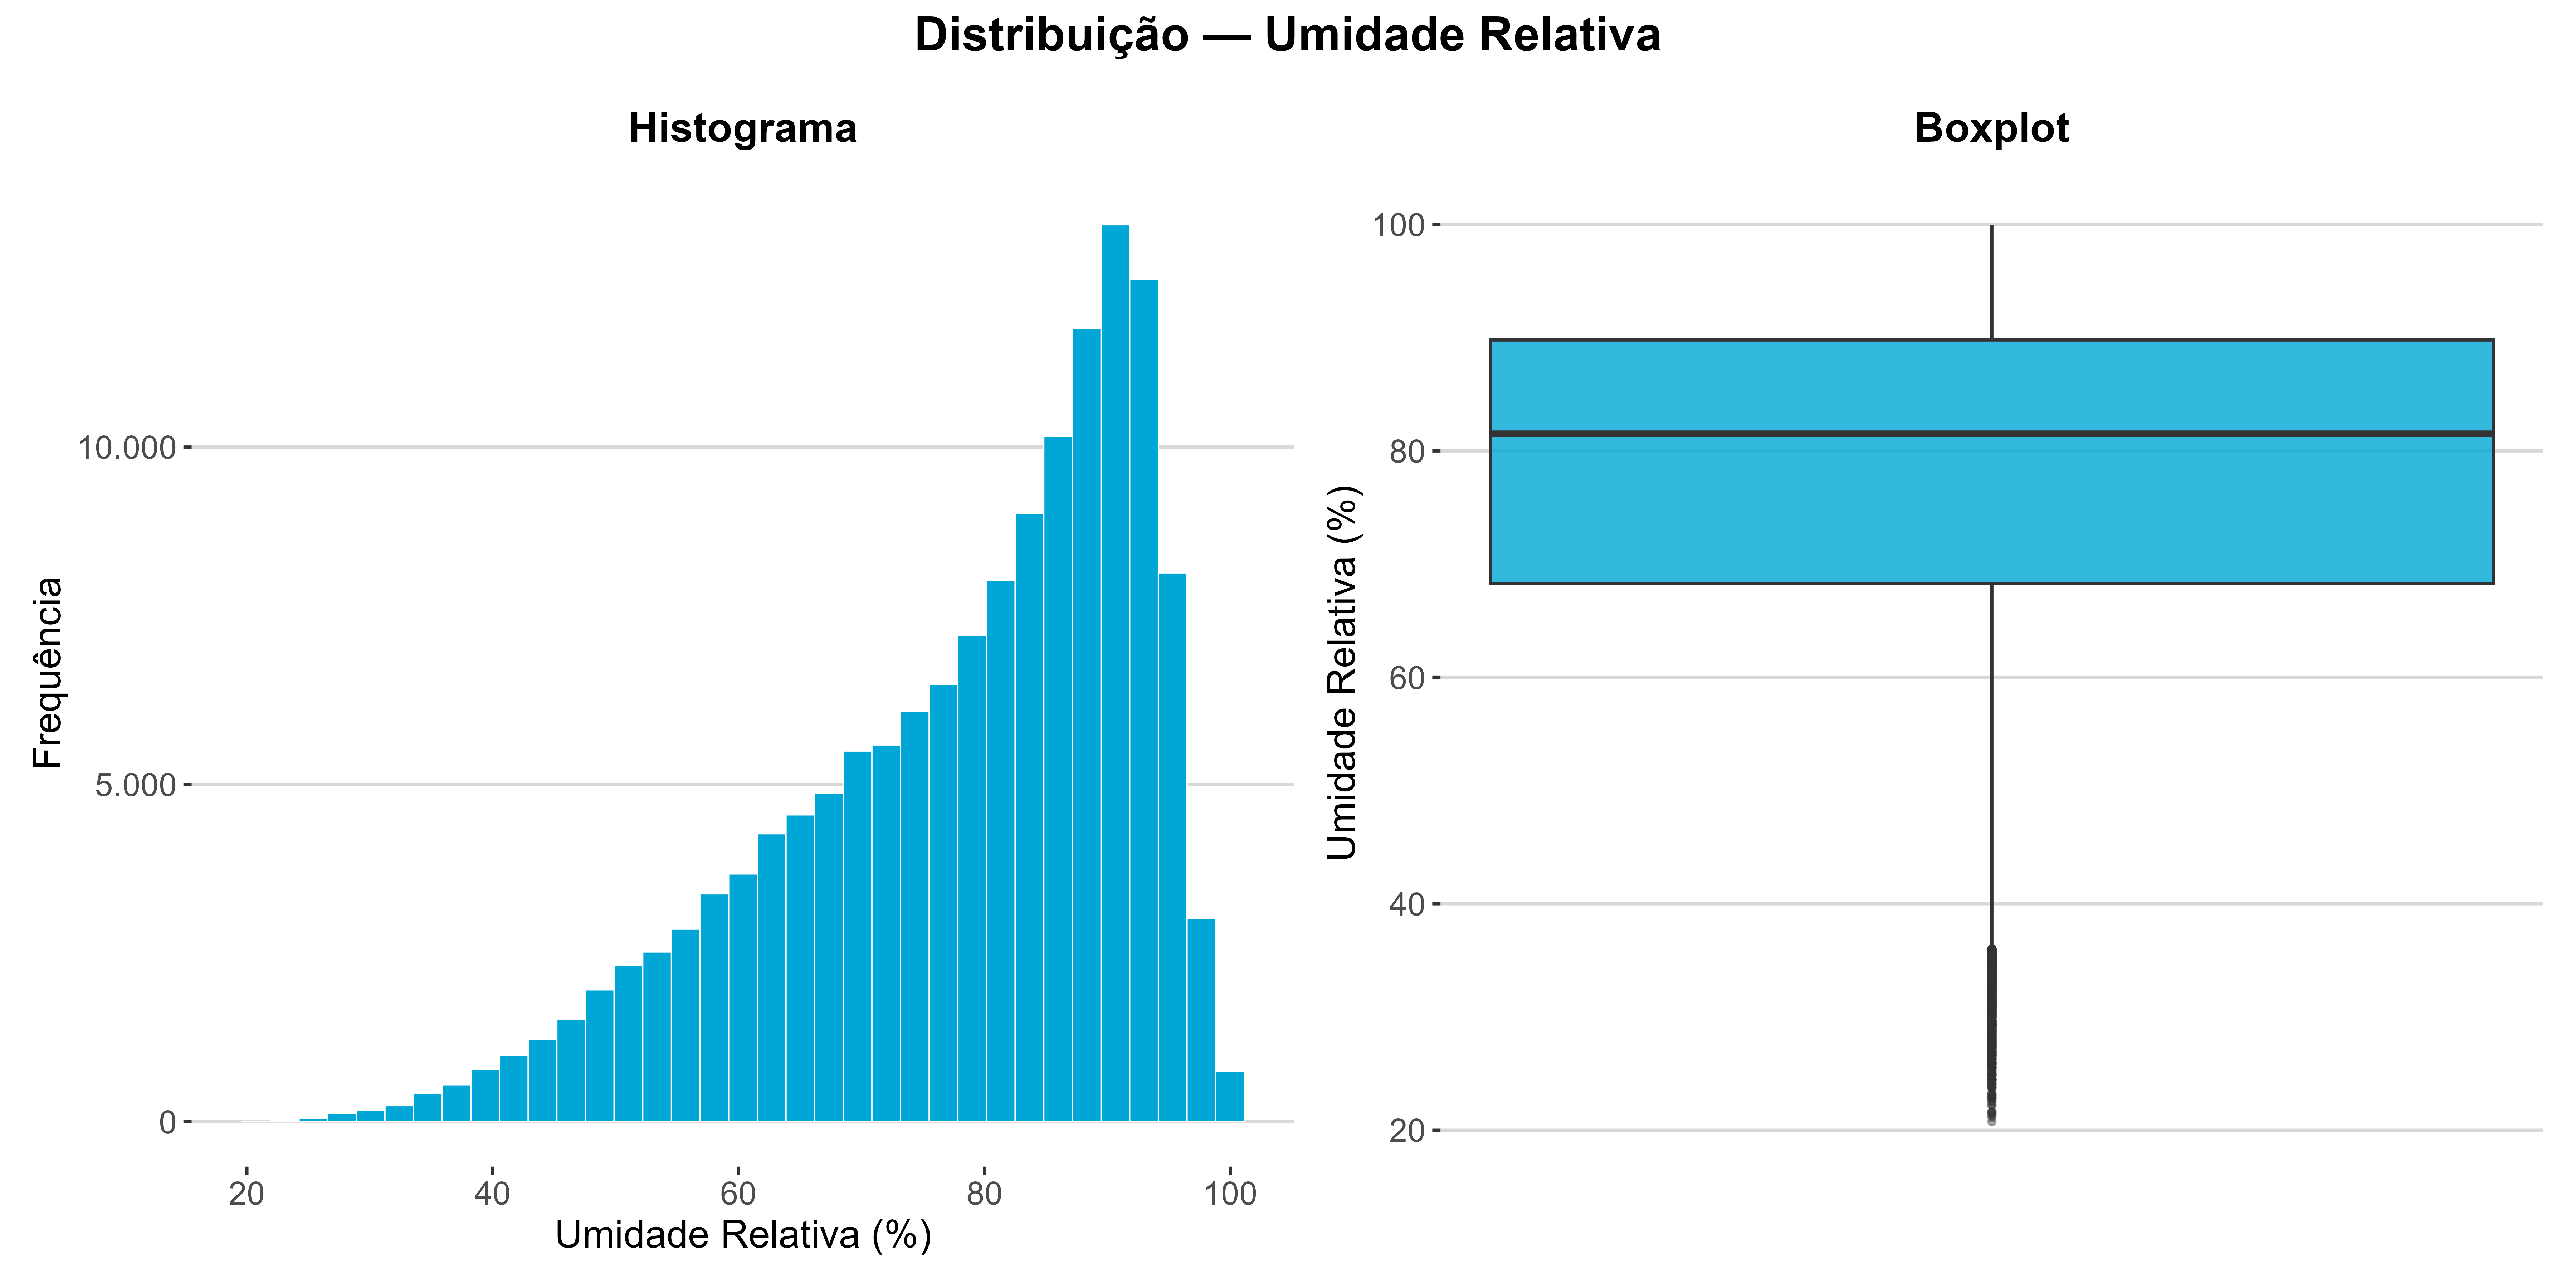
\includegraphics[keepaspectratio]{resultados/UmidadRel/04_umidadrel_distribuicao.png}}

}

\caption{Distribuição da Umidade Relativa}

\end{figure}%

\paragraph{Principais Achados}\label{principais-achados-1}

A umidade relativa mantém-se \textbf{persistentemente elevada} ao longo
de toda a série, com valores horários raramente abaixo de 40\% e mediana
próxima a 80\%. Na escala mensal, oscila entre \textasciitilde70\%
(meses mais secos de inverno) e \textasciitilde87\% (verão/outono), sem
tendência temporal clara.

A distribuição é \textbf{assimétrica à esquerda} (cauda inferior), com a
grande maioria das observações concentradas entre 70\% e 100\%. Isso
indica que Niterói raramente experimenta condições de ar seco, o que é
esperado para uma cidade litorânea. O comportamento é inversamente
correlacionado com a temperatura, conforme evidenciado nas análises
conjuntas.

\subsubsection{Precipitação}\label{precipitauxe7uxe3o}

\begin{figure}[H]

{\centering \pandocbounded{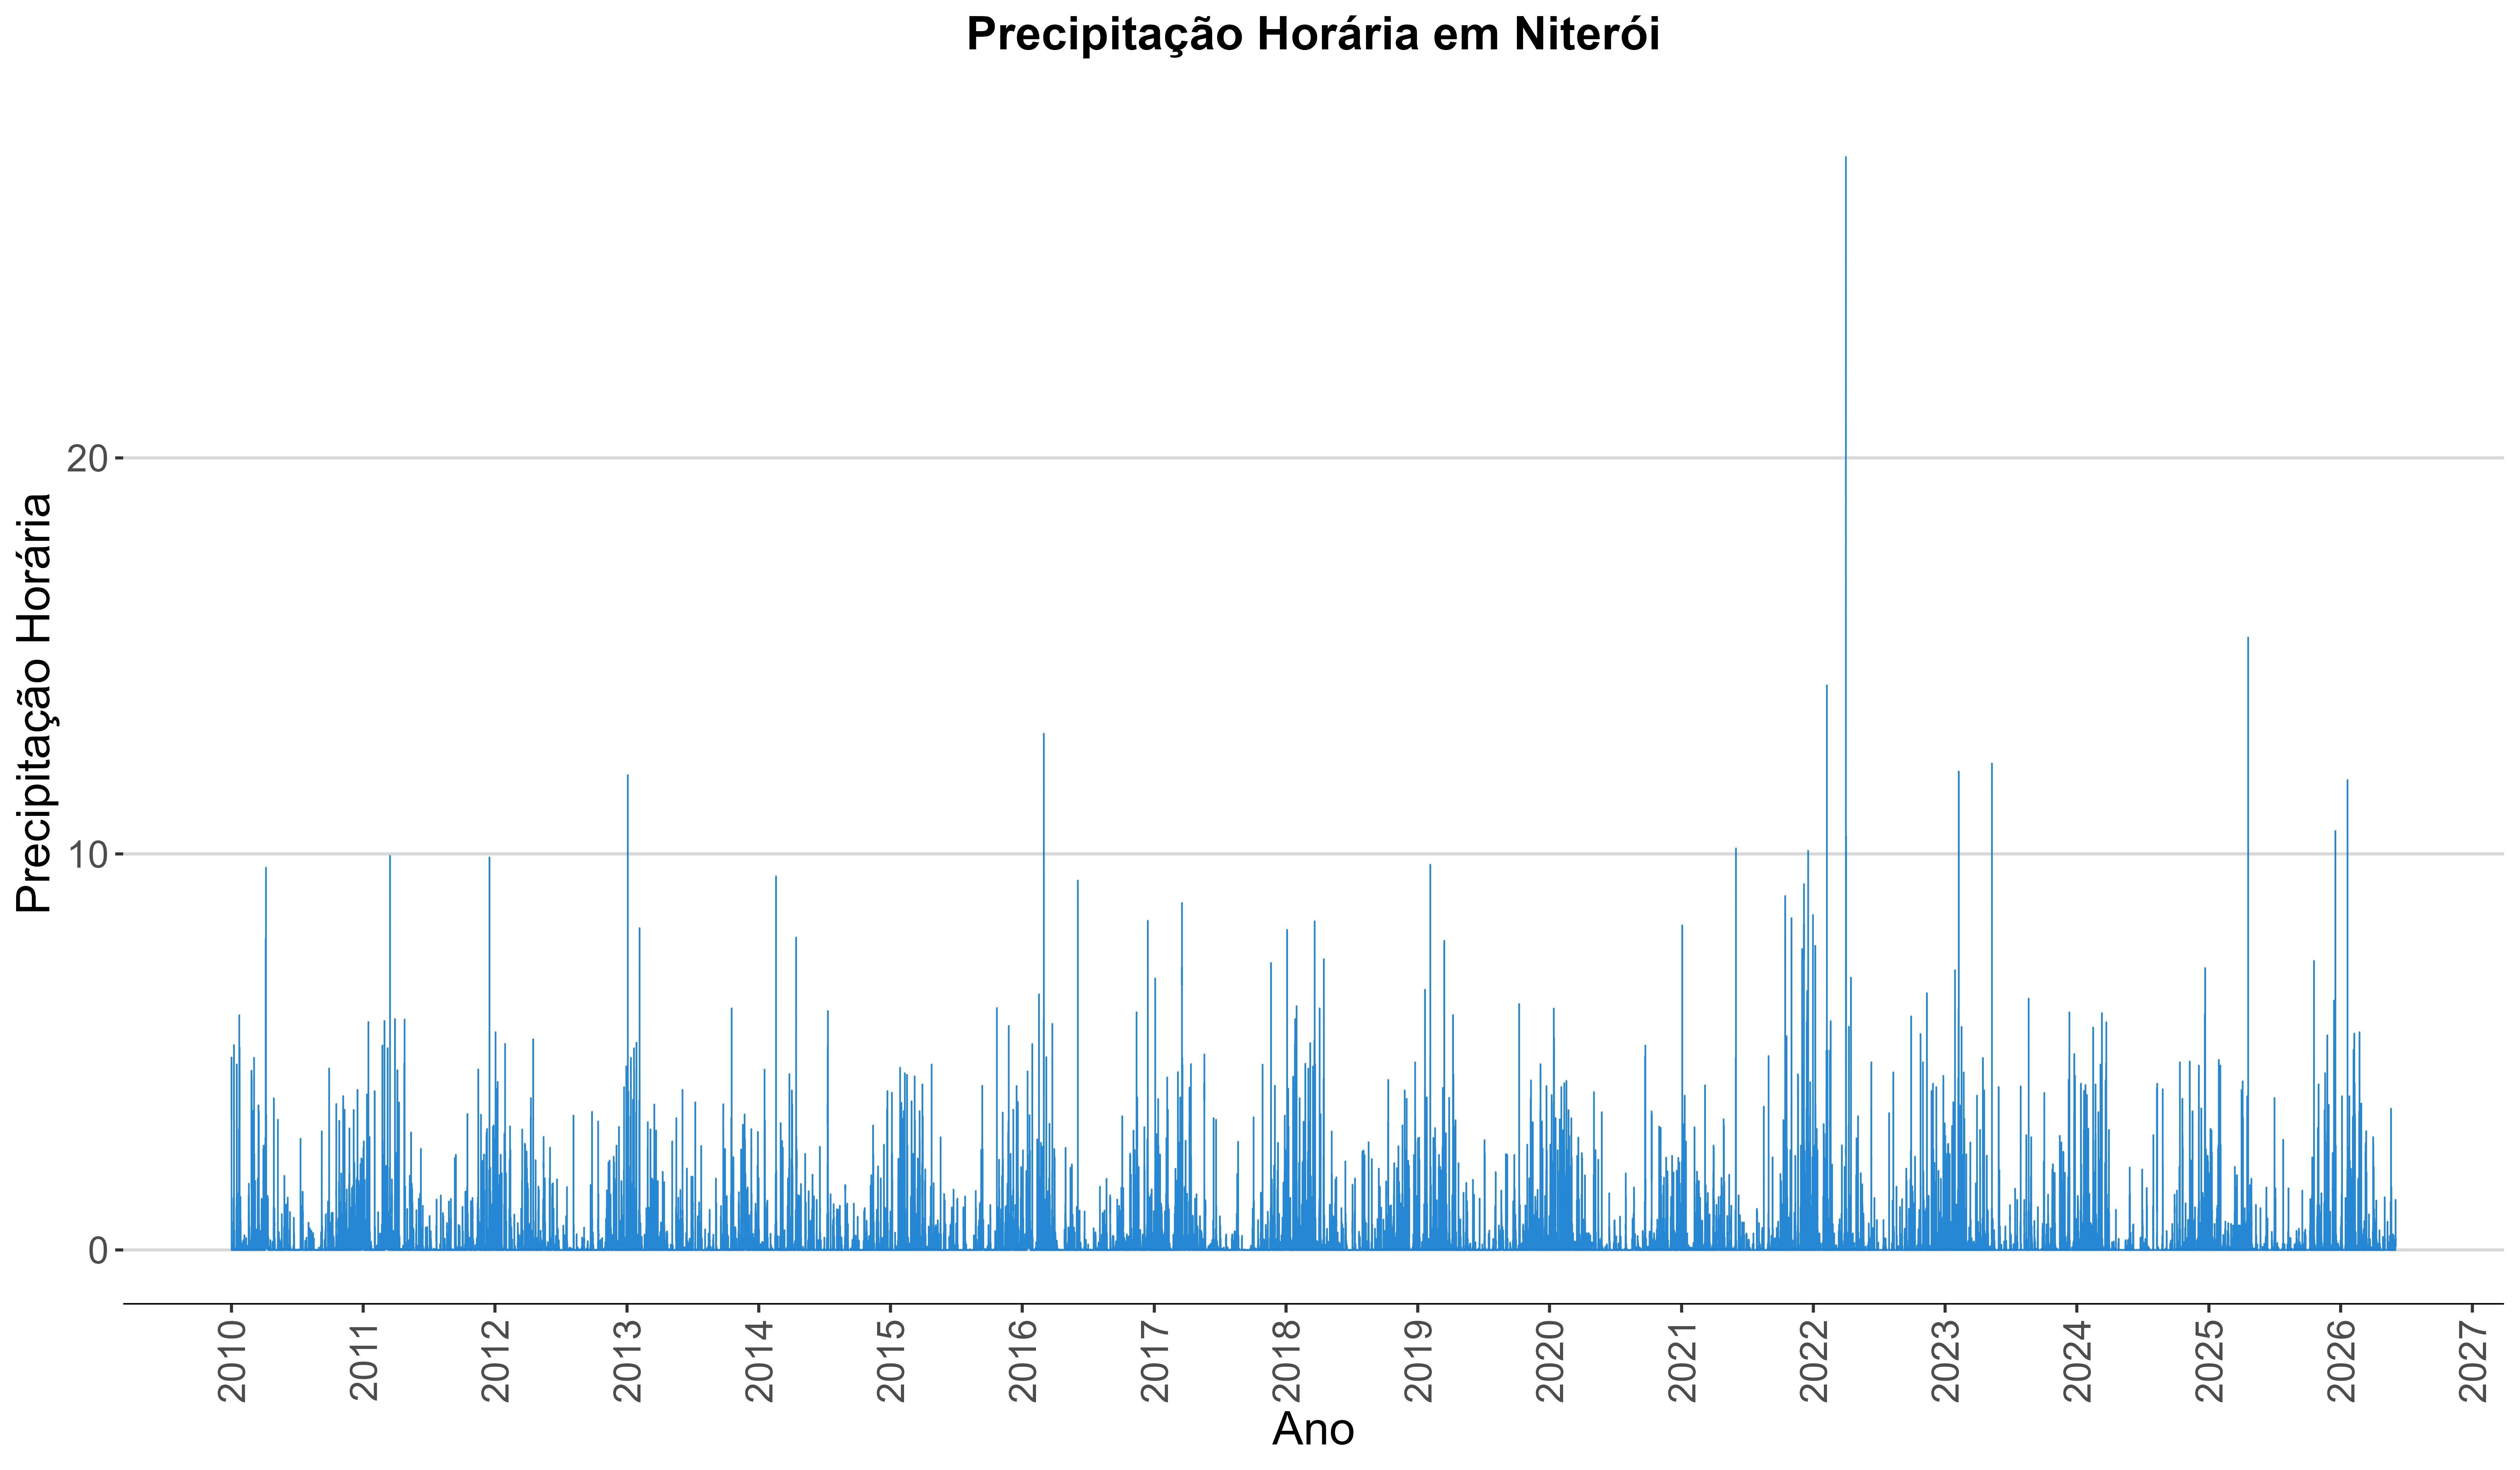
\includegraphics[keepaspectratio]{resultados/Precipitacao/00_precipitacao_horaria.png}}

}

\caption{Precipitação Horária}

\end{figure}%

\begin{figure}[H]

{\centering \pandocbounded{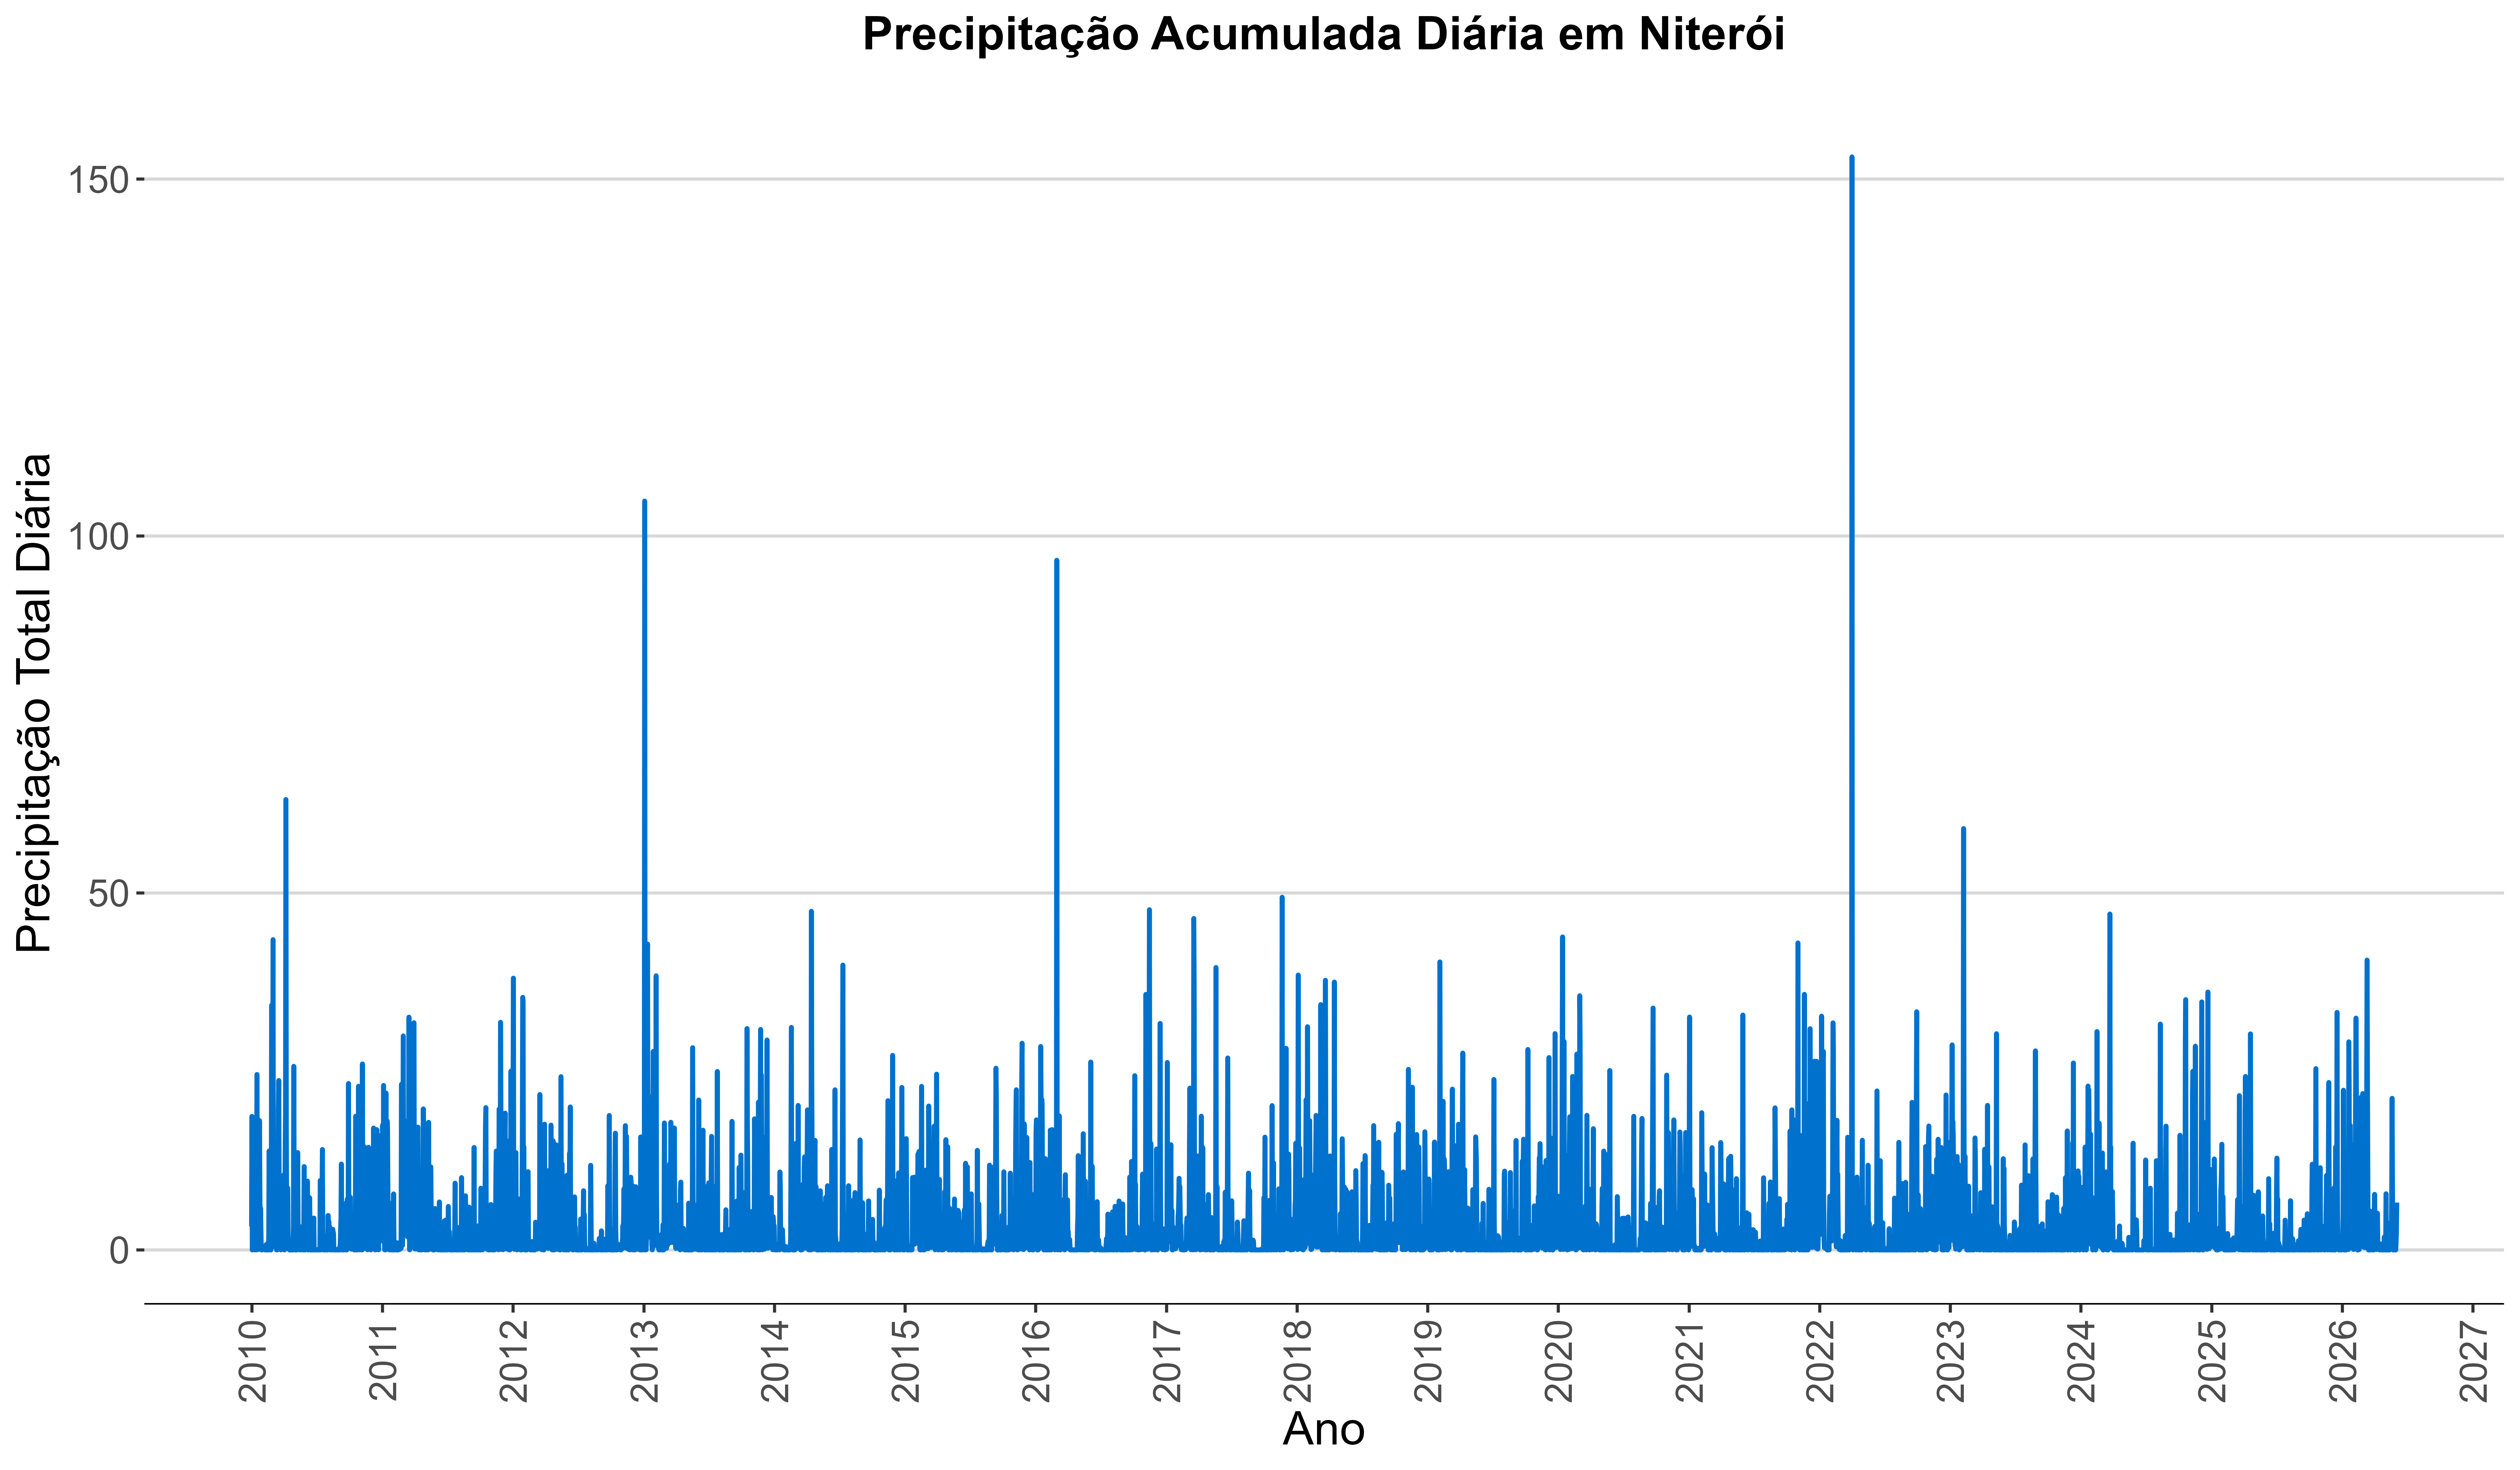
\includegraphics[keepaspectratio]{resultados/Precipitacao/01_precipitacao_total_diaria.png}}

}

\caption{Precipitação Acumulada Diária}

\end{figure}%

\begin{figure}[H]

{\centering \pandocbounded{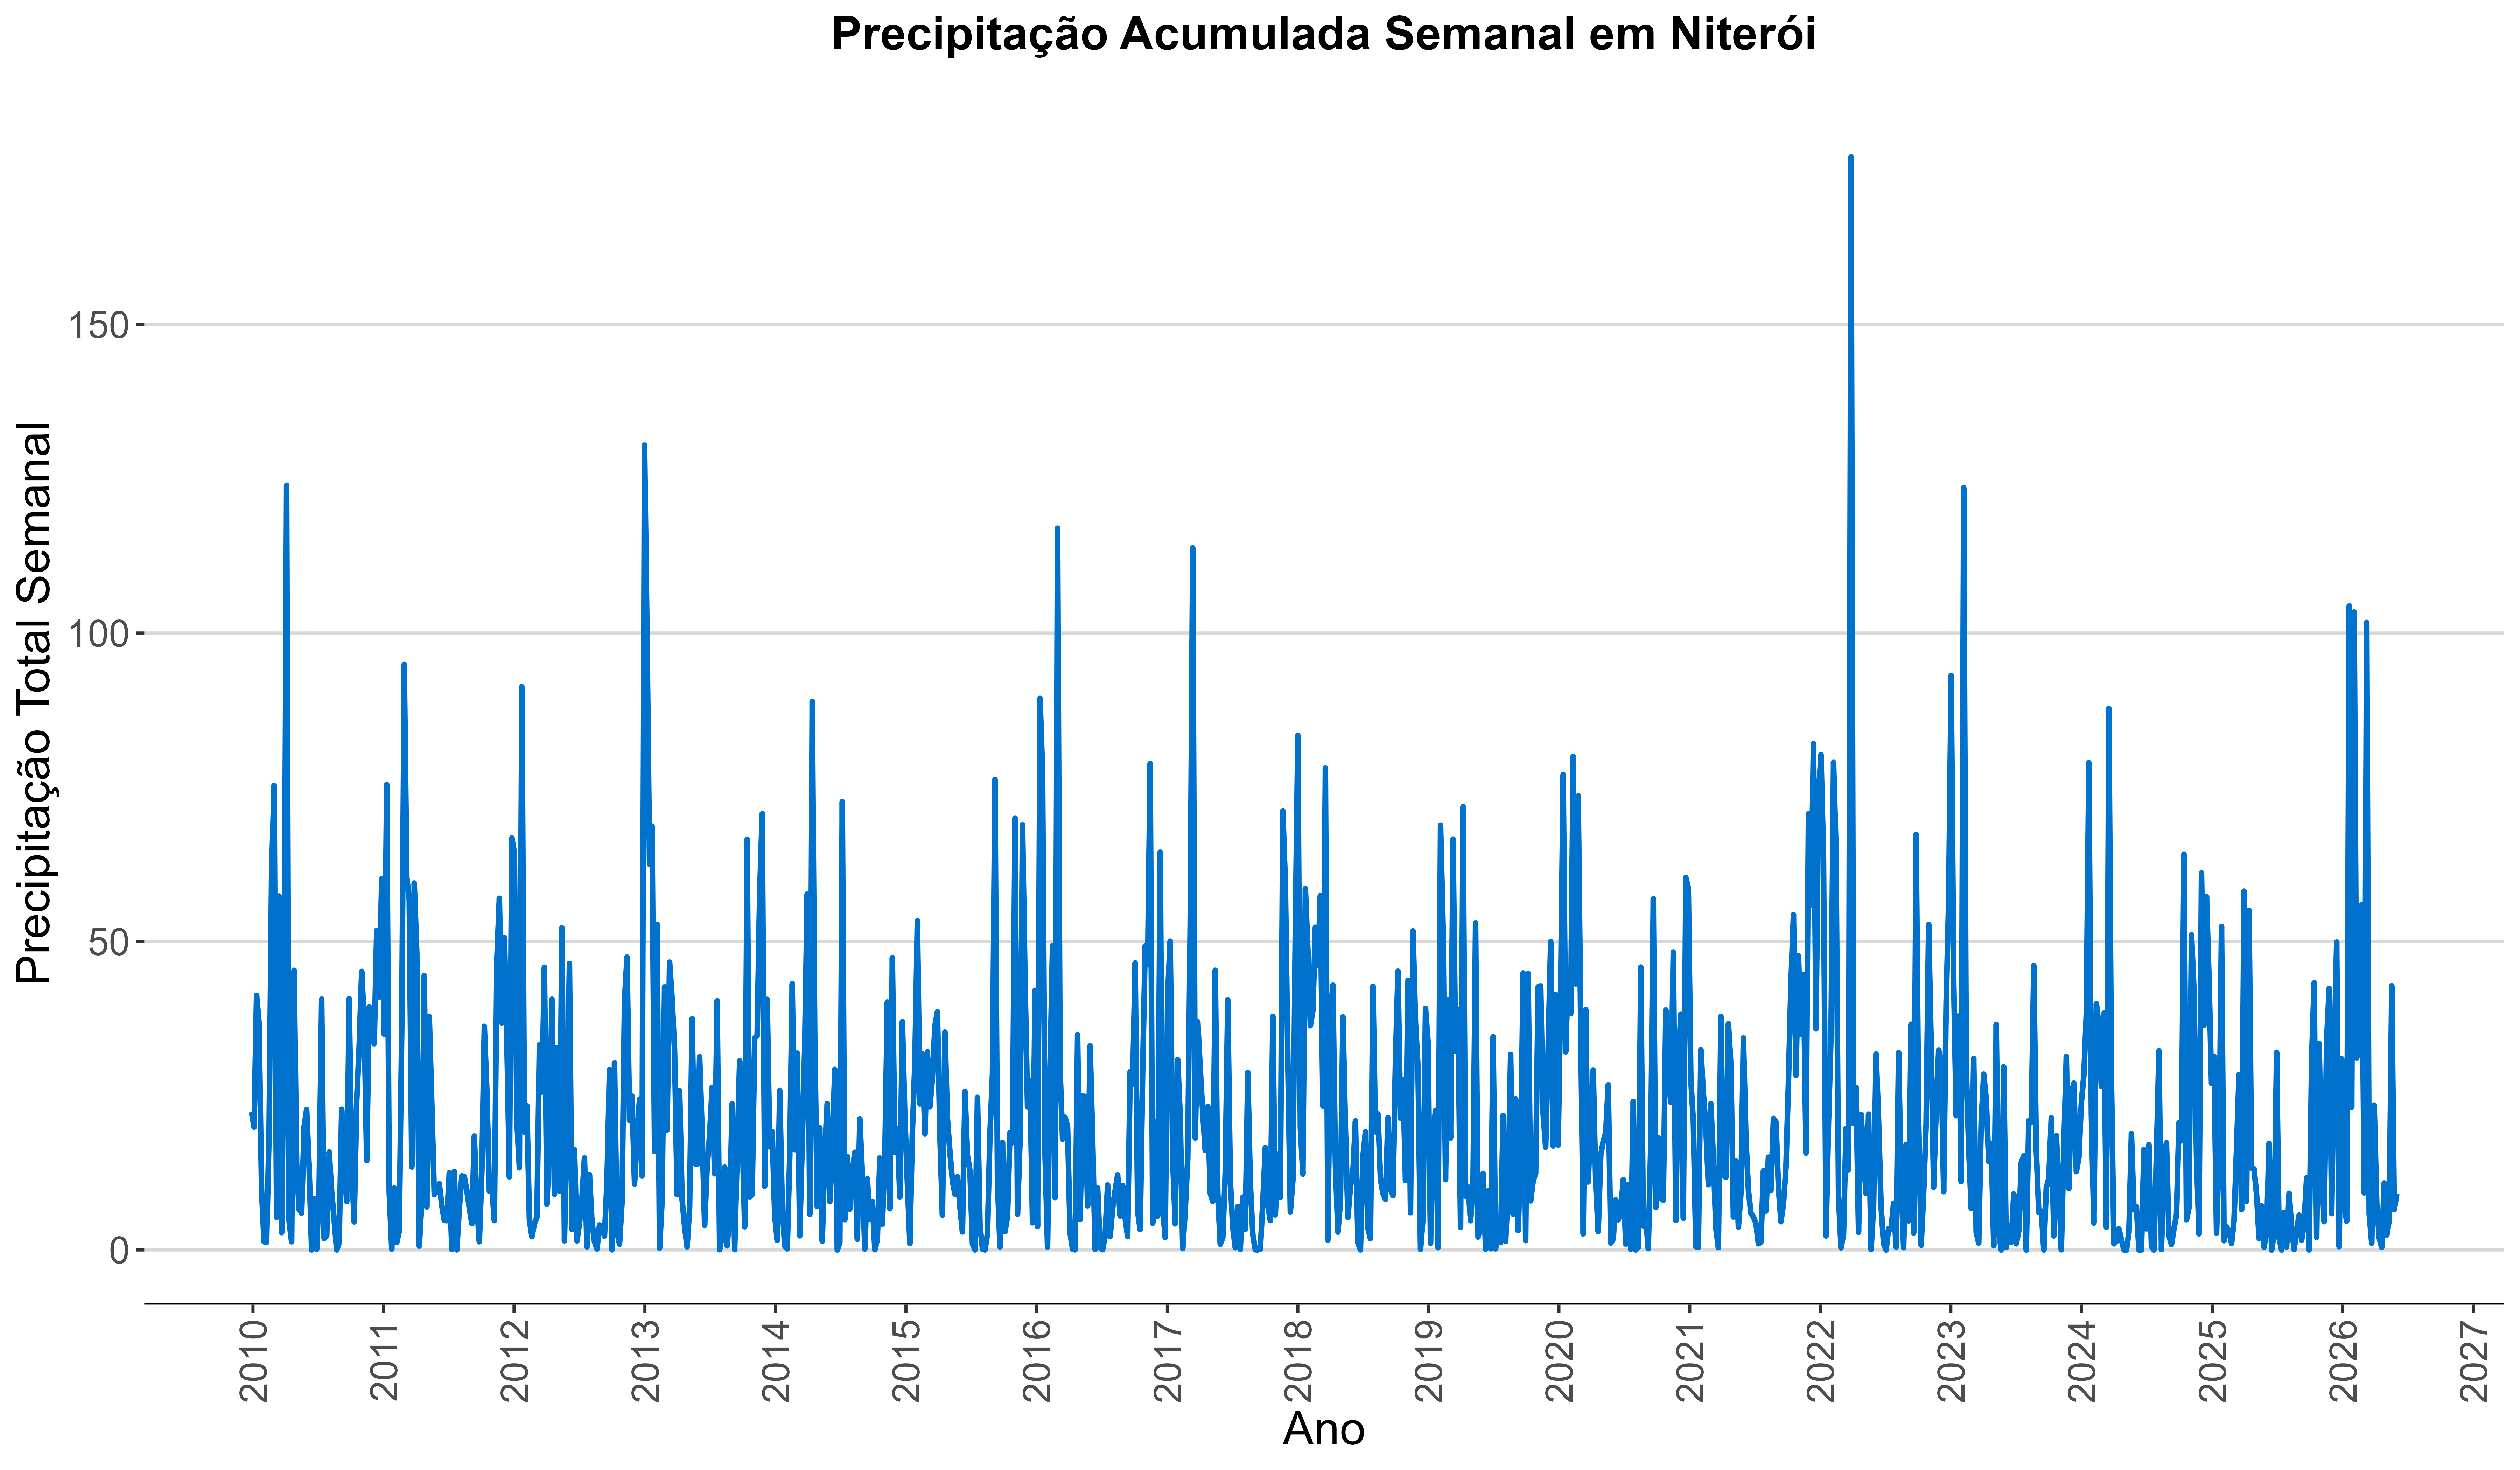
\includegraphics[keepaspectratio]{resultados/Precipitacao/02_precipitacao_total_semanal.png}}

}

\caption{Precipitação Acumulada Semanal}

\end{figure}%

\begin{figure}[H]

{\centering \pandocbounded{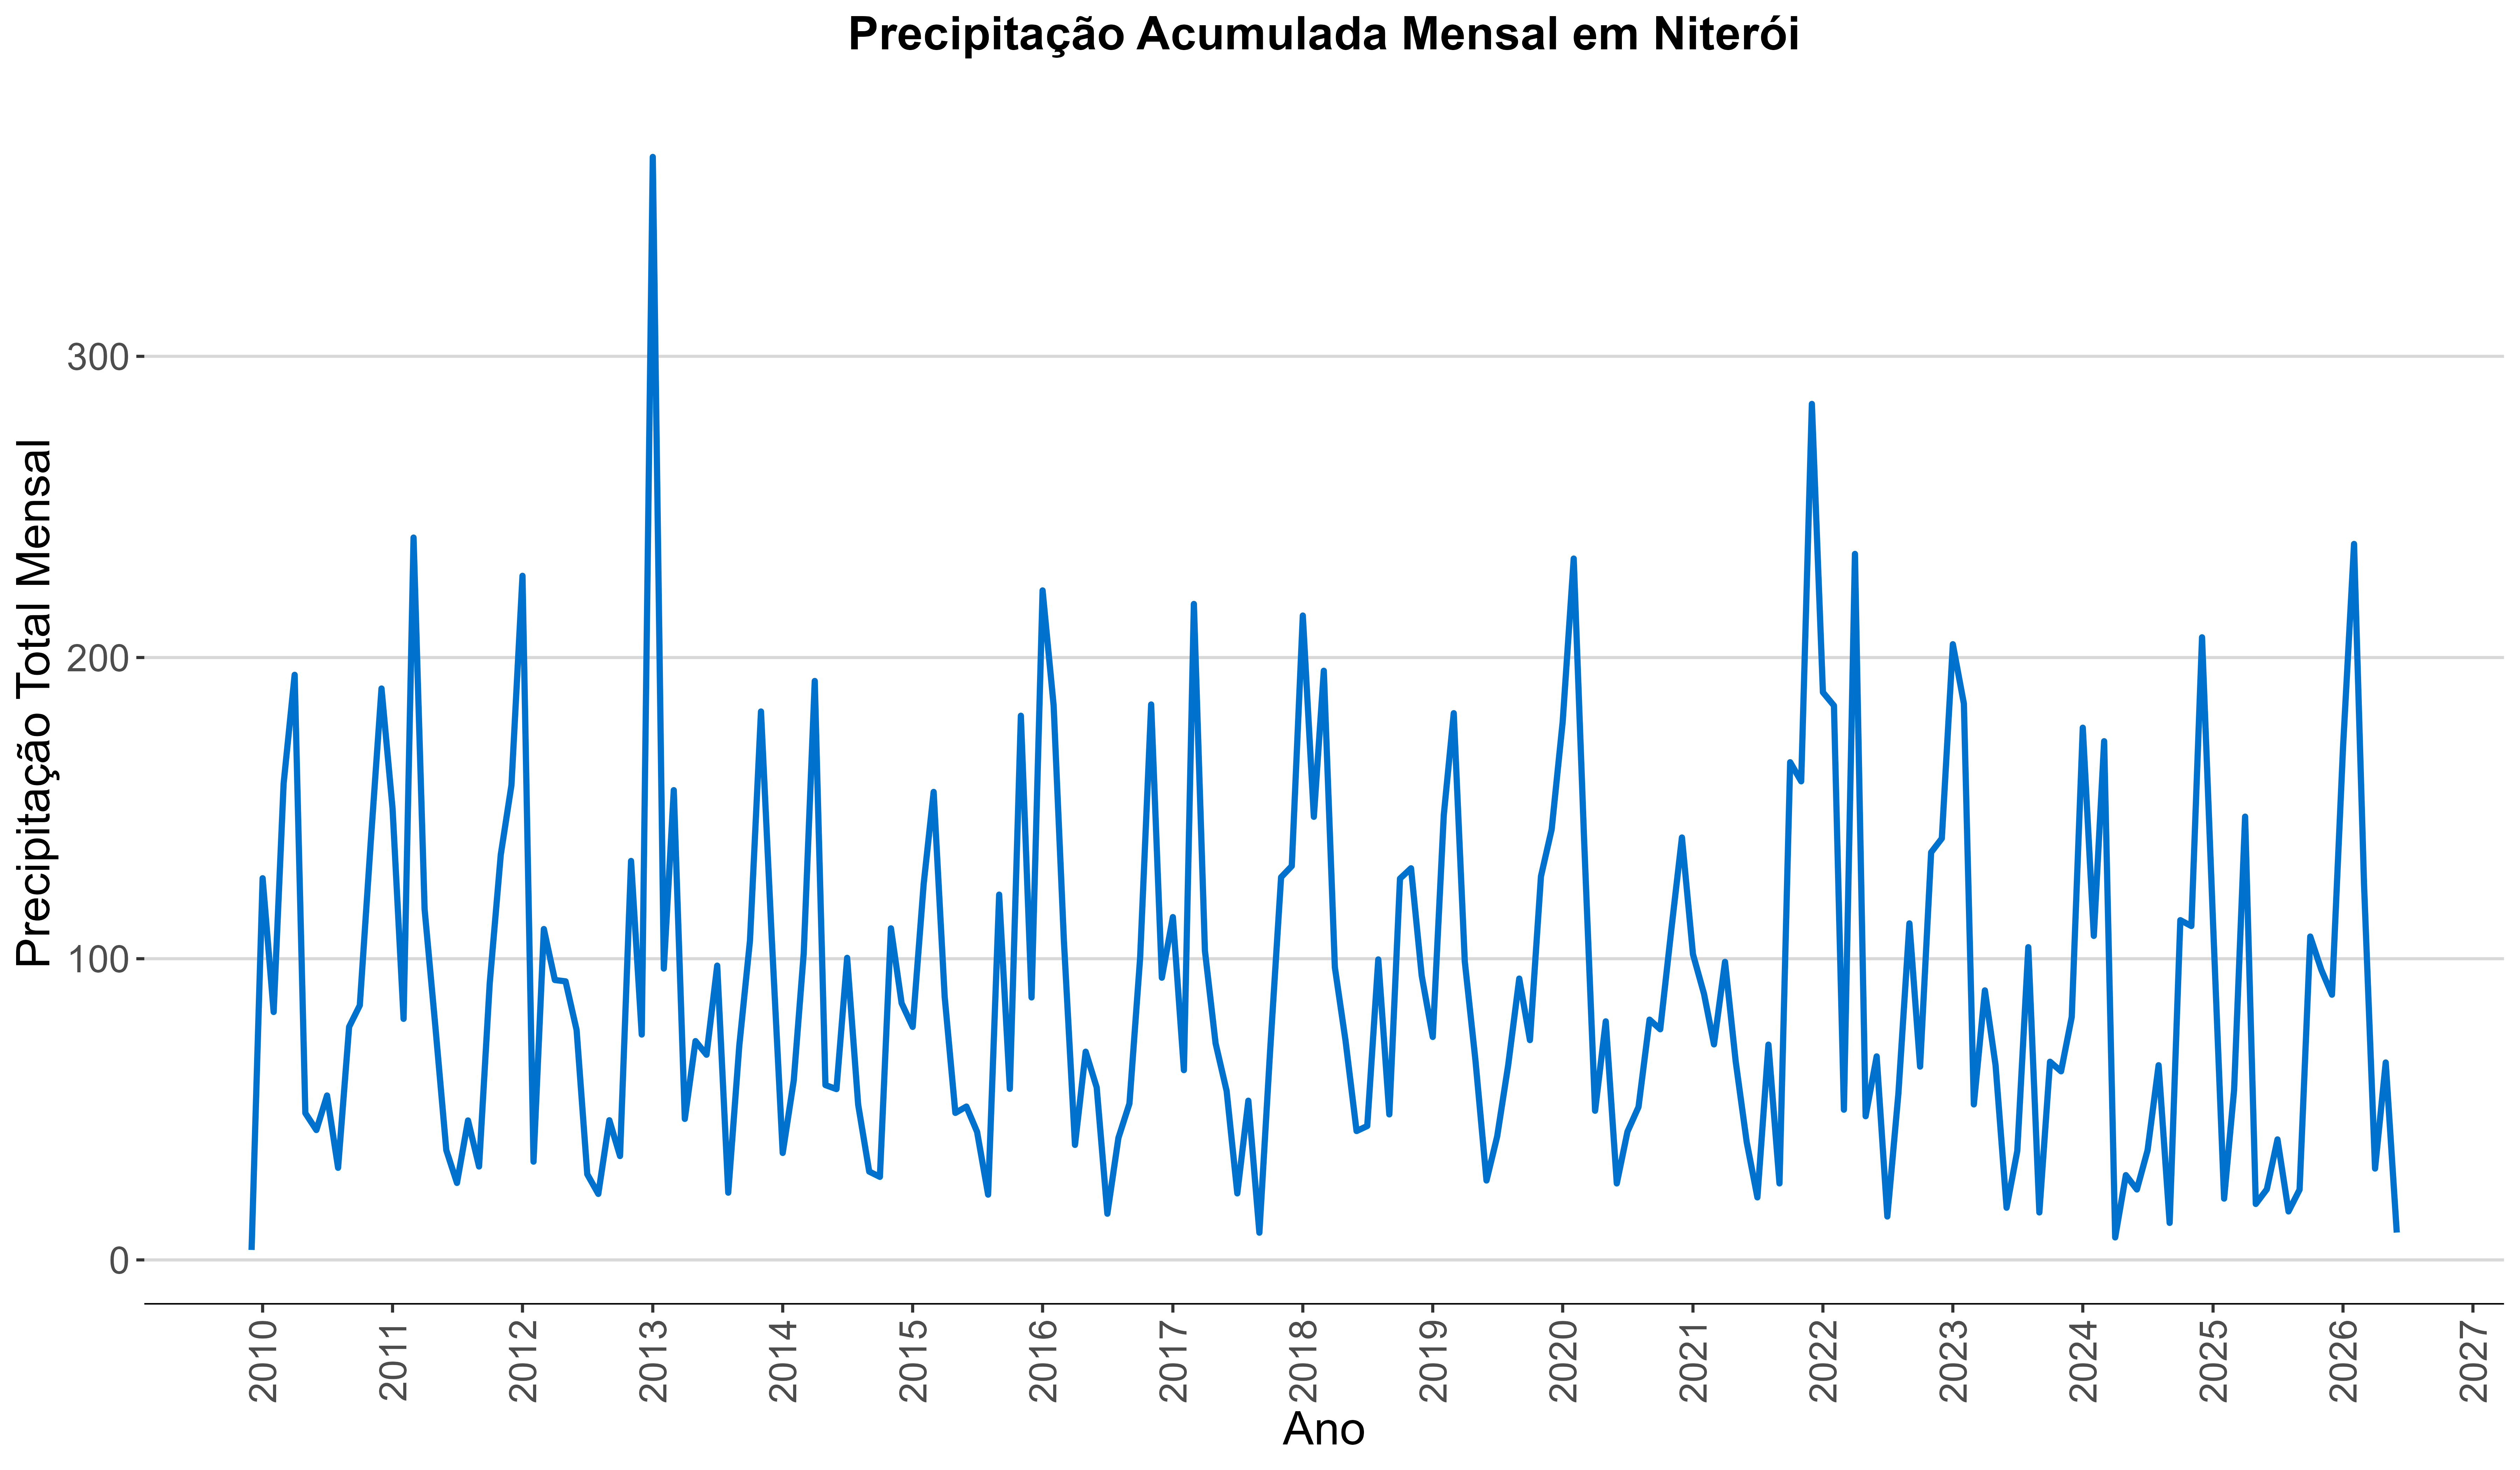
\includegraphics[keepaspectratio]{resultados/Precipitacao/03_precipitacao_total_mensal.png}}

}

\caption{Precipitação Acumulada Mensal}

\end{figure}%

\begin{figure}[H]

{\centering \pandocbounded{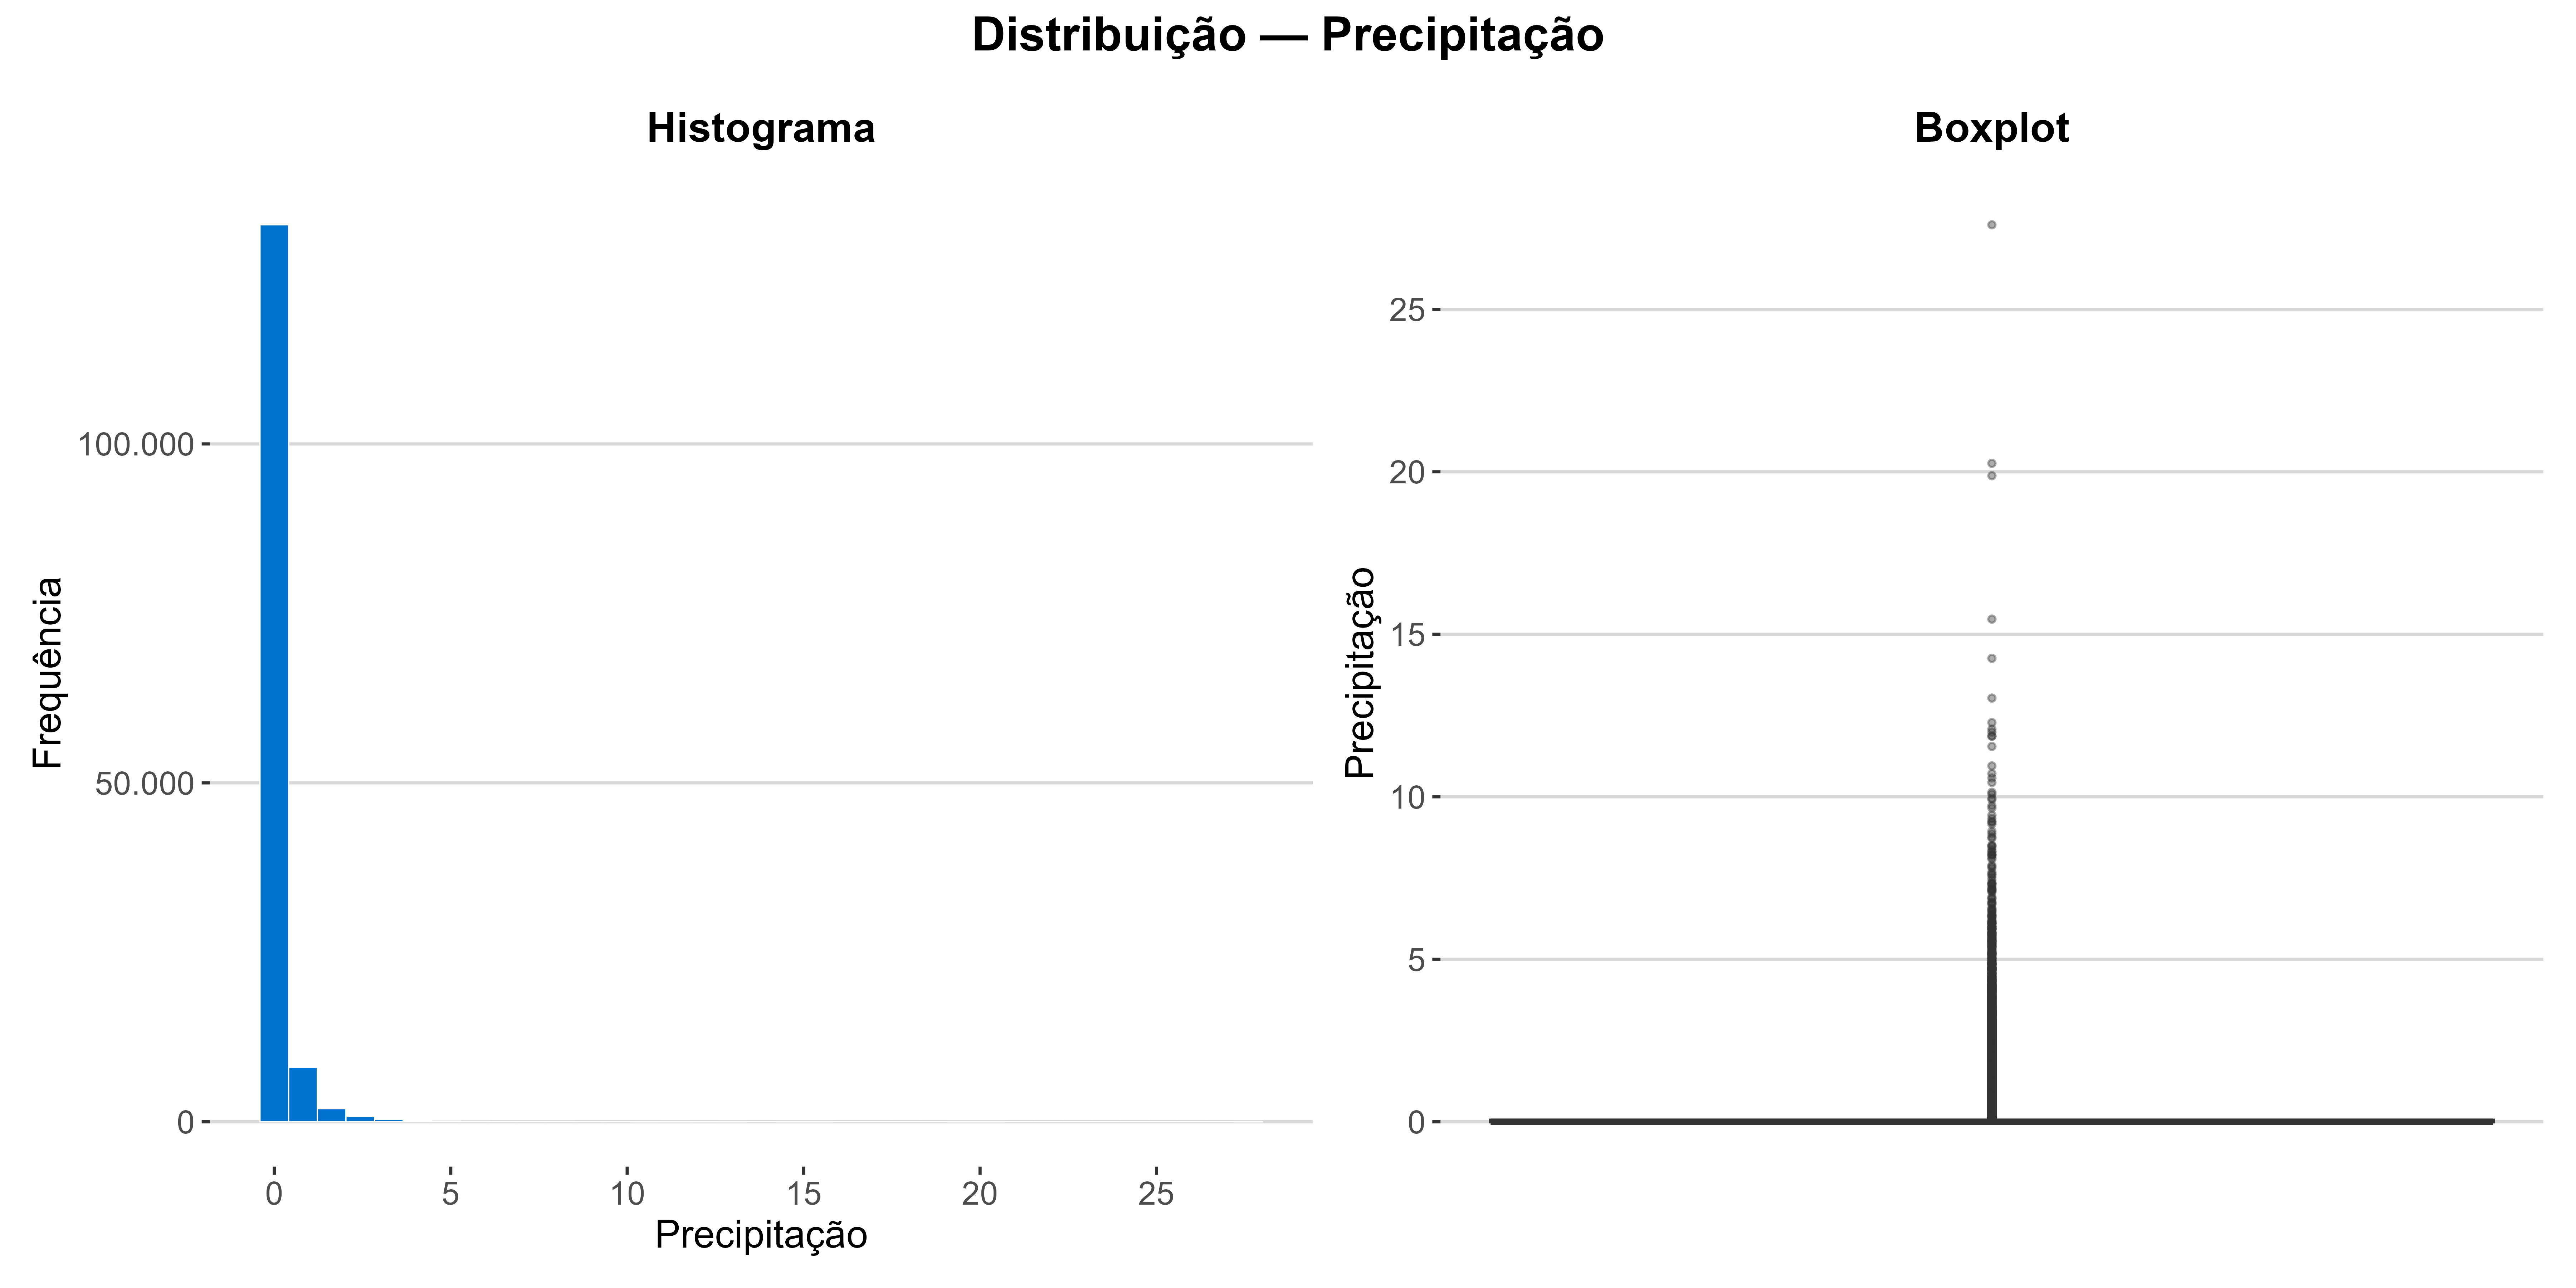
\includegraphics[keepaspectratio]{resultados/Precipitacao/04_precipitacao_distribuicao.png}}

}

\caption{Distribuição da Precipitação}

\end{figure}%

\paragraph{Principais Achados}\label{principais-achados-2}

A precipitação apresenta o padrão \textbf{mais singular} de todas as
variáveis: a esmagadora maioria das observações horárias é zero, com
eventos intensos e pontuais que chegam a superar 10 mm/h. O histograma
confirma essa característica com distribuição fortemente concentrada em
zero e cauda extremamente longa à direita.

Na escala diária e semanal, destacam-se eventos extremos --- dias com
acumulado superior a 50 mm aparecem em vários anos, com um pico notável
próximo a 150 mm/dia em 2022. Na escala mensal, os meses de verão
(especialmente novembro a março) concentram os maiores volumes, enquanto
o inverno tende a ser significativamente mais seco, refletindo o regime
tropical/subtropical da região.

\subsubsection{Velocidade do Vento}\label{velocidade-do-vento}

\begin{figure}[H]

{\centering \pandocbounded{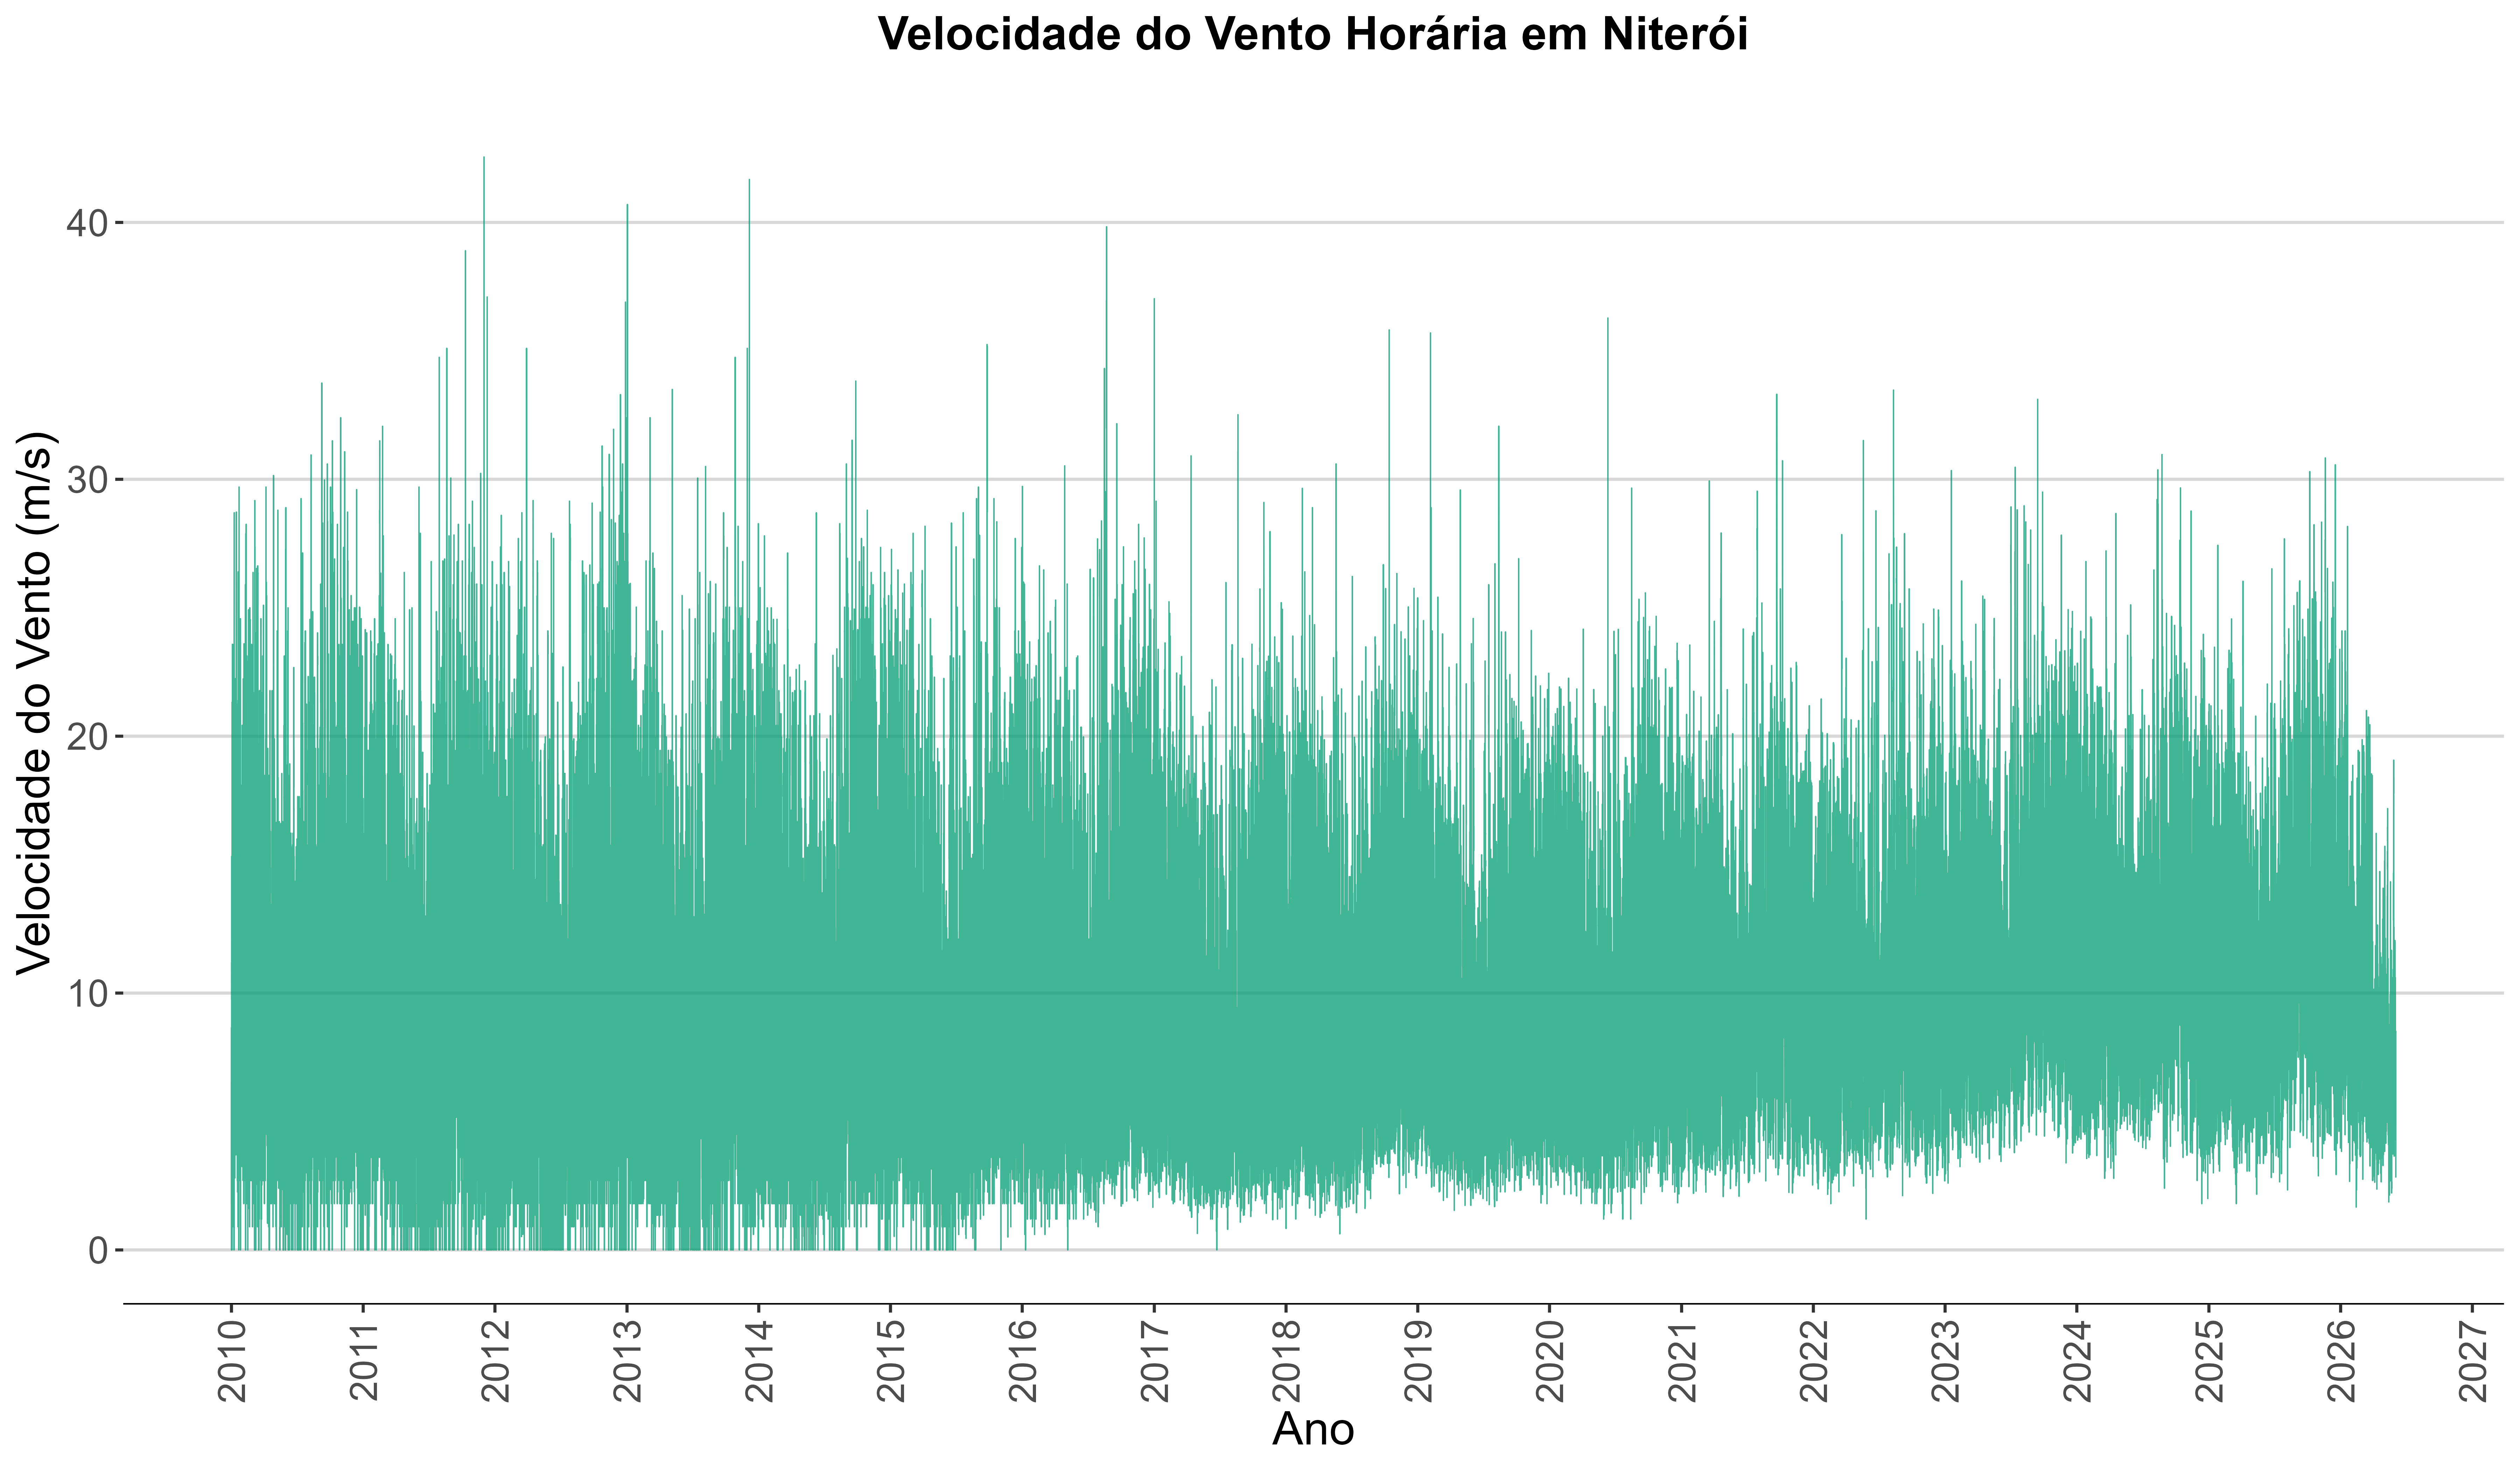
\includegraphics[keepaspectratio]{resultados/VelocVento/00_velocidade_vento_horaria.png}}

}

\caption{Velocidade do Vento Horária}

\end{figure}%

\begin{figure}[H]

{\centering \pandocbounded{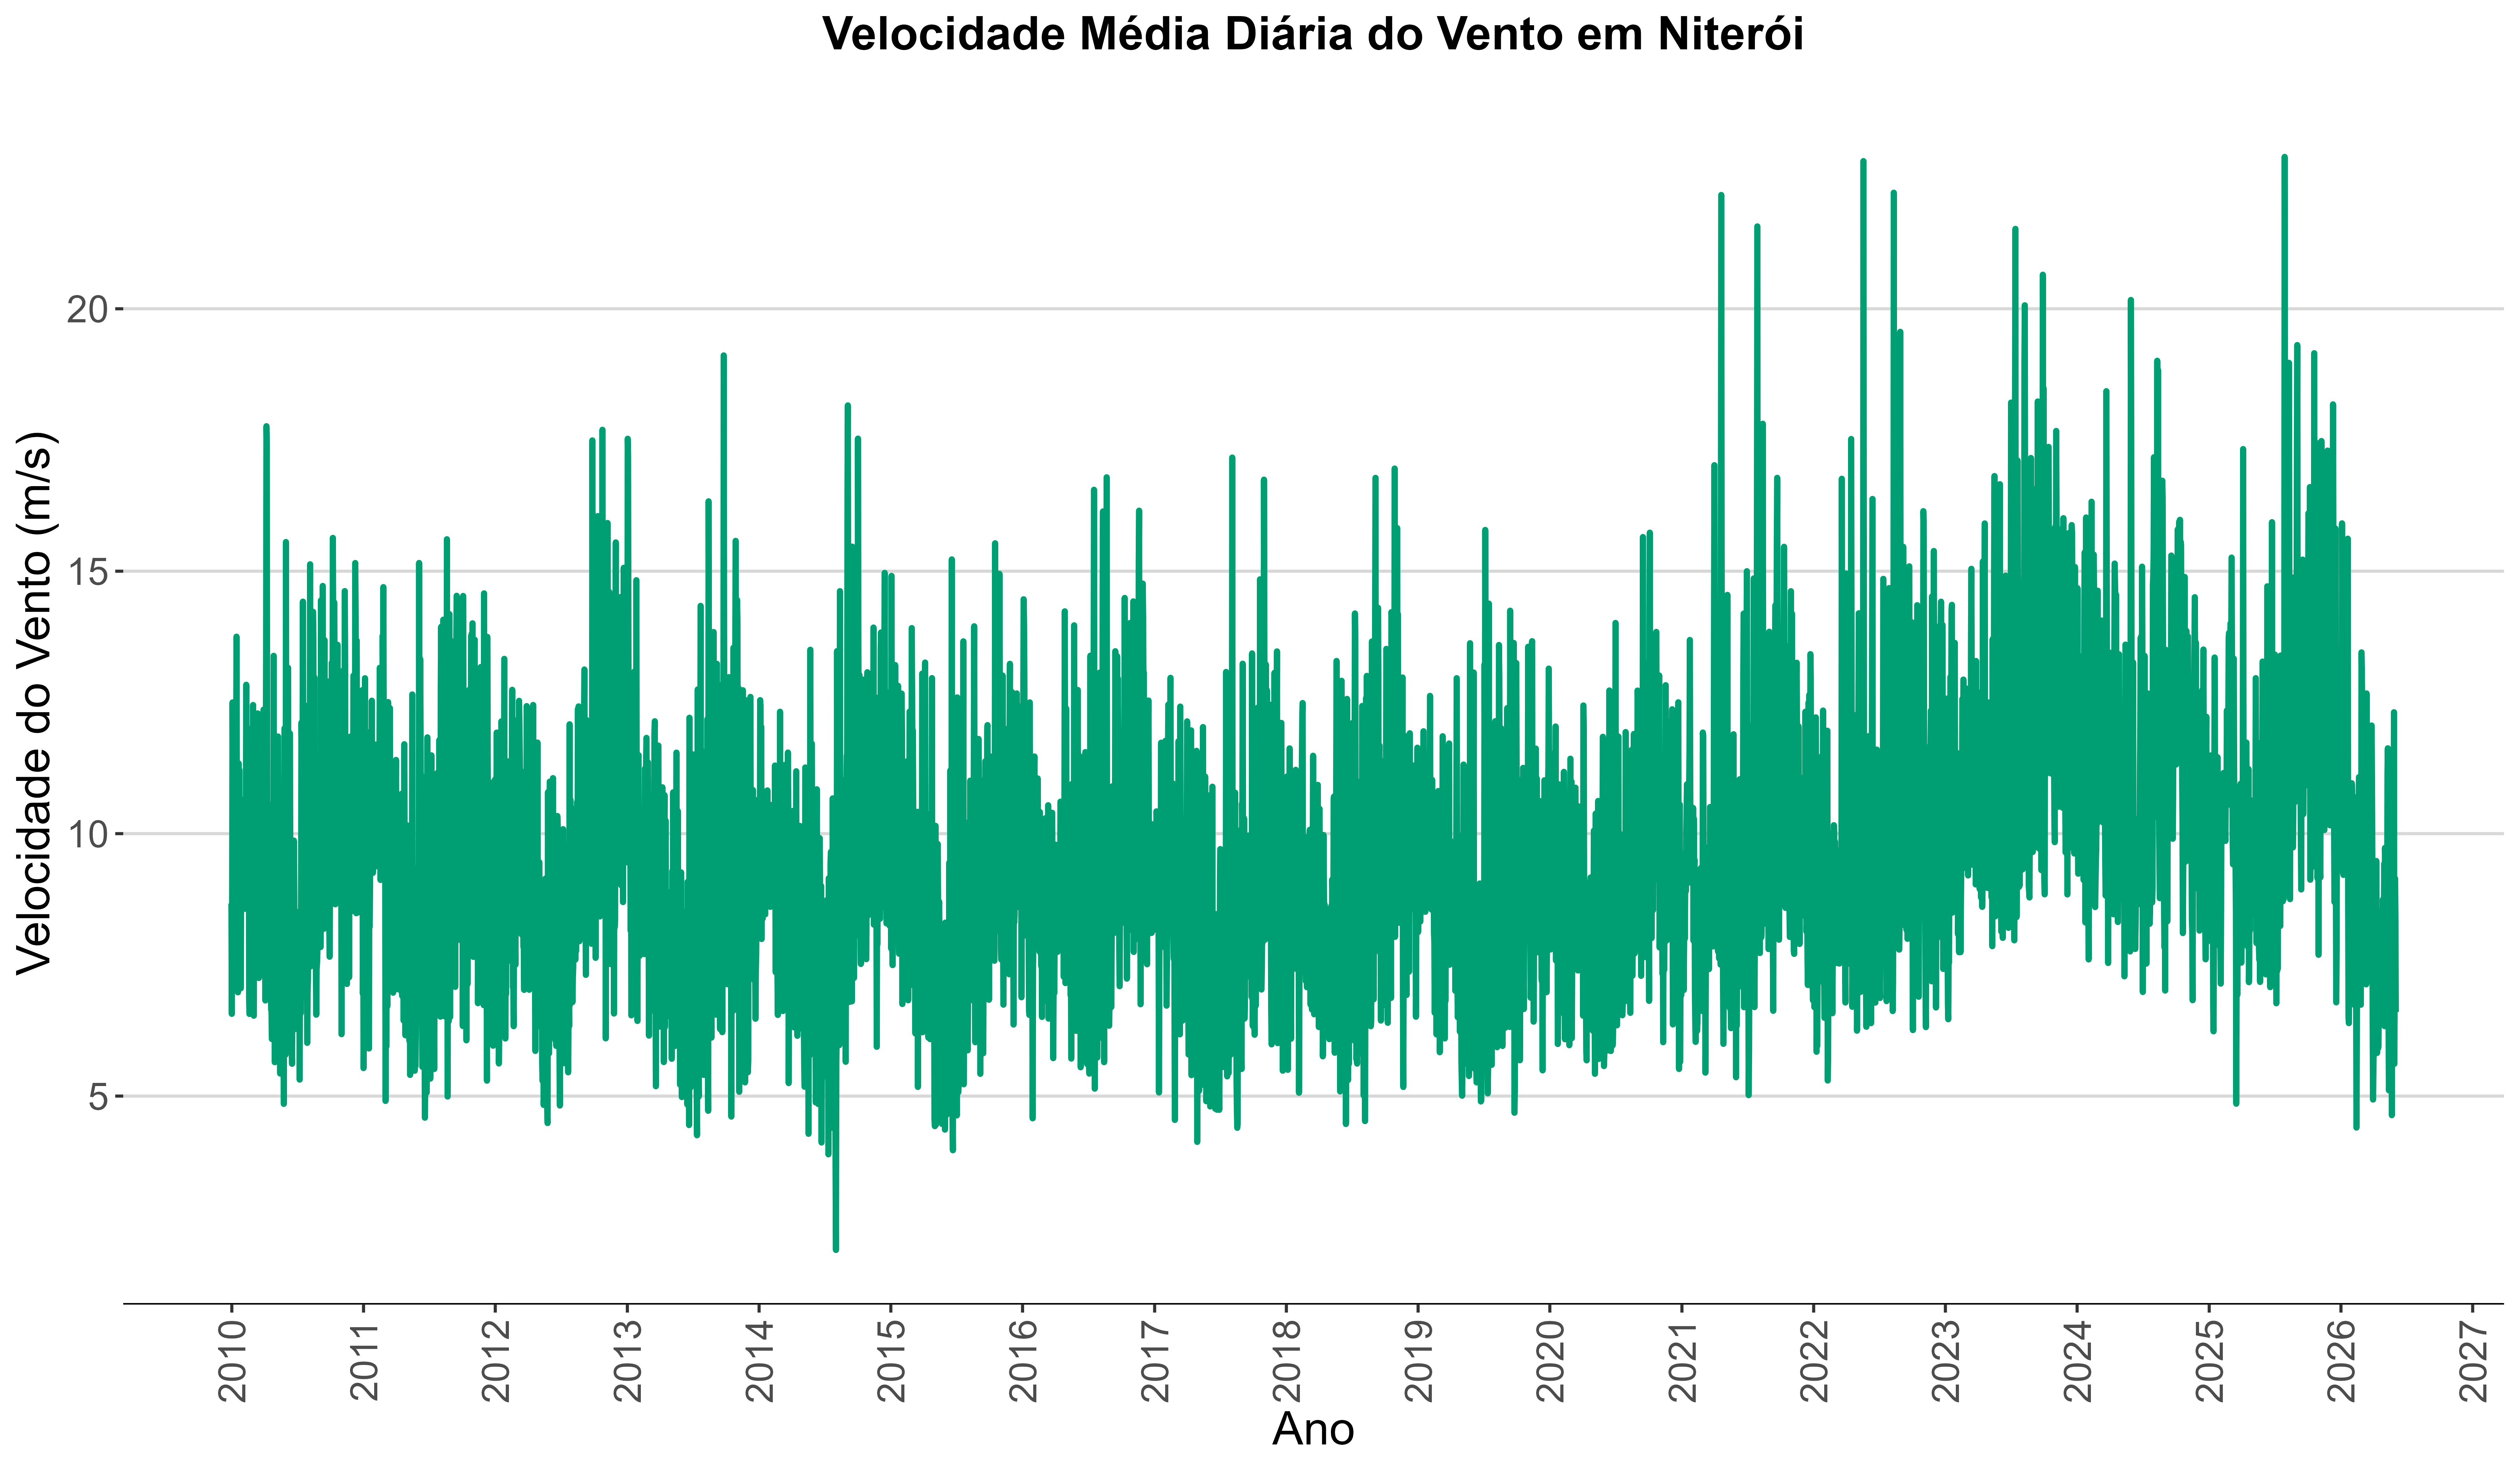
\includegraphics[keepaspectratio]{resultados/VelocVento/01_velocidade_vento_media_diaria.png}}

}

\caption{Velocidade Média Diária do Vento}

\end{figure}%

\begin{figure}[H]

{\centering \pandocbounded{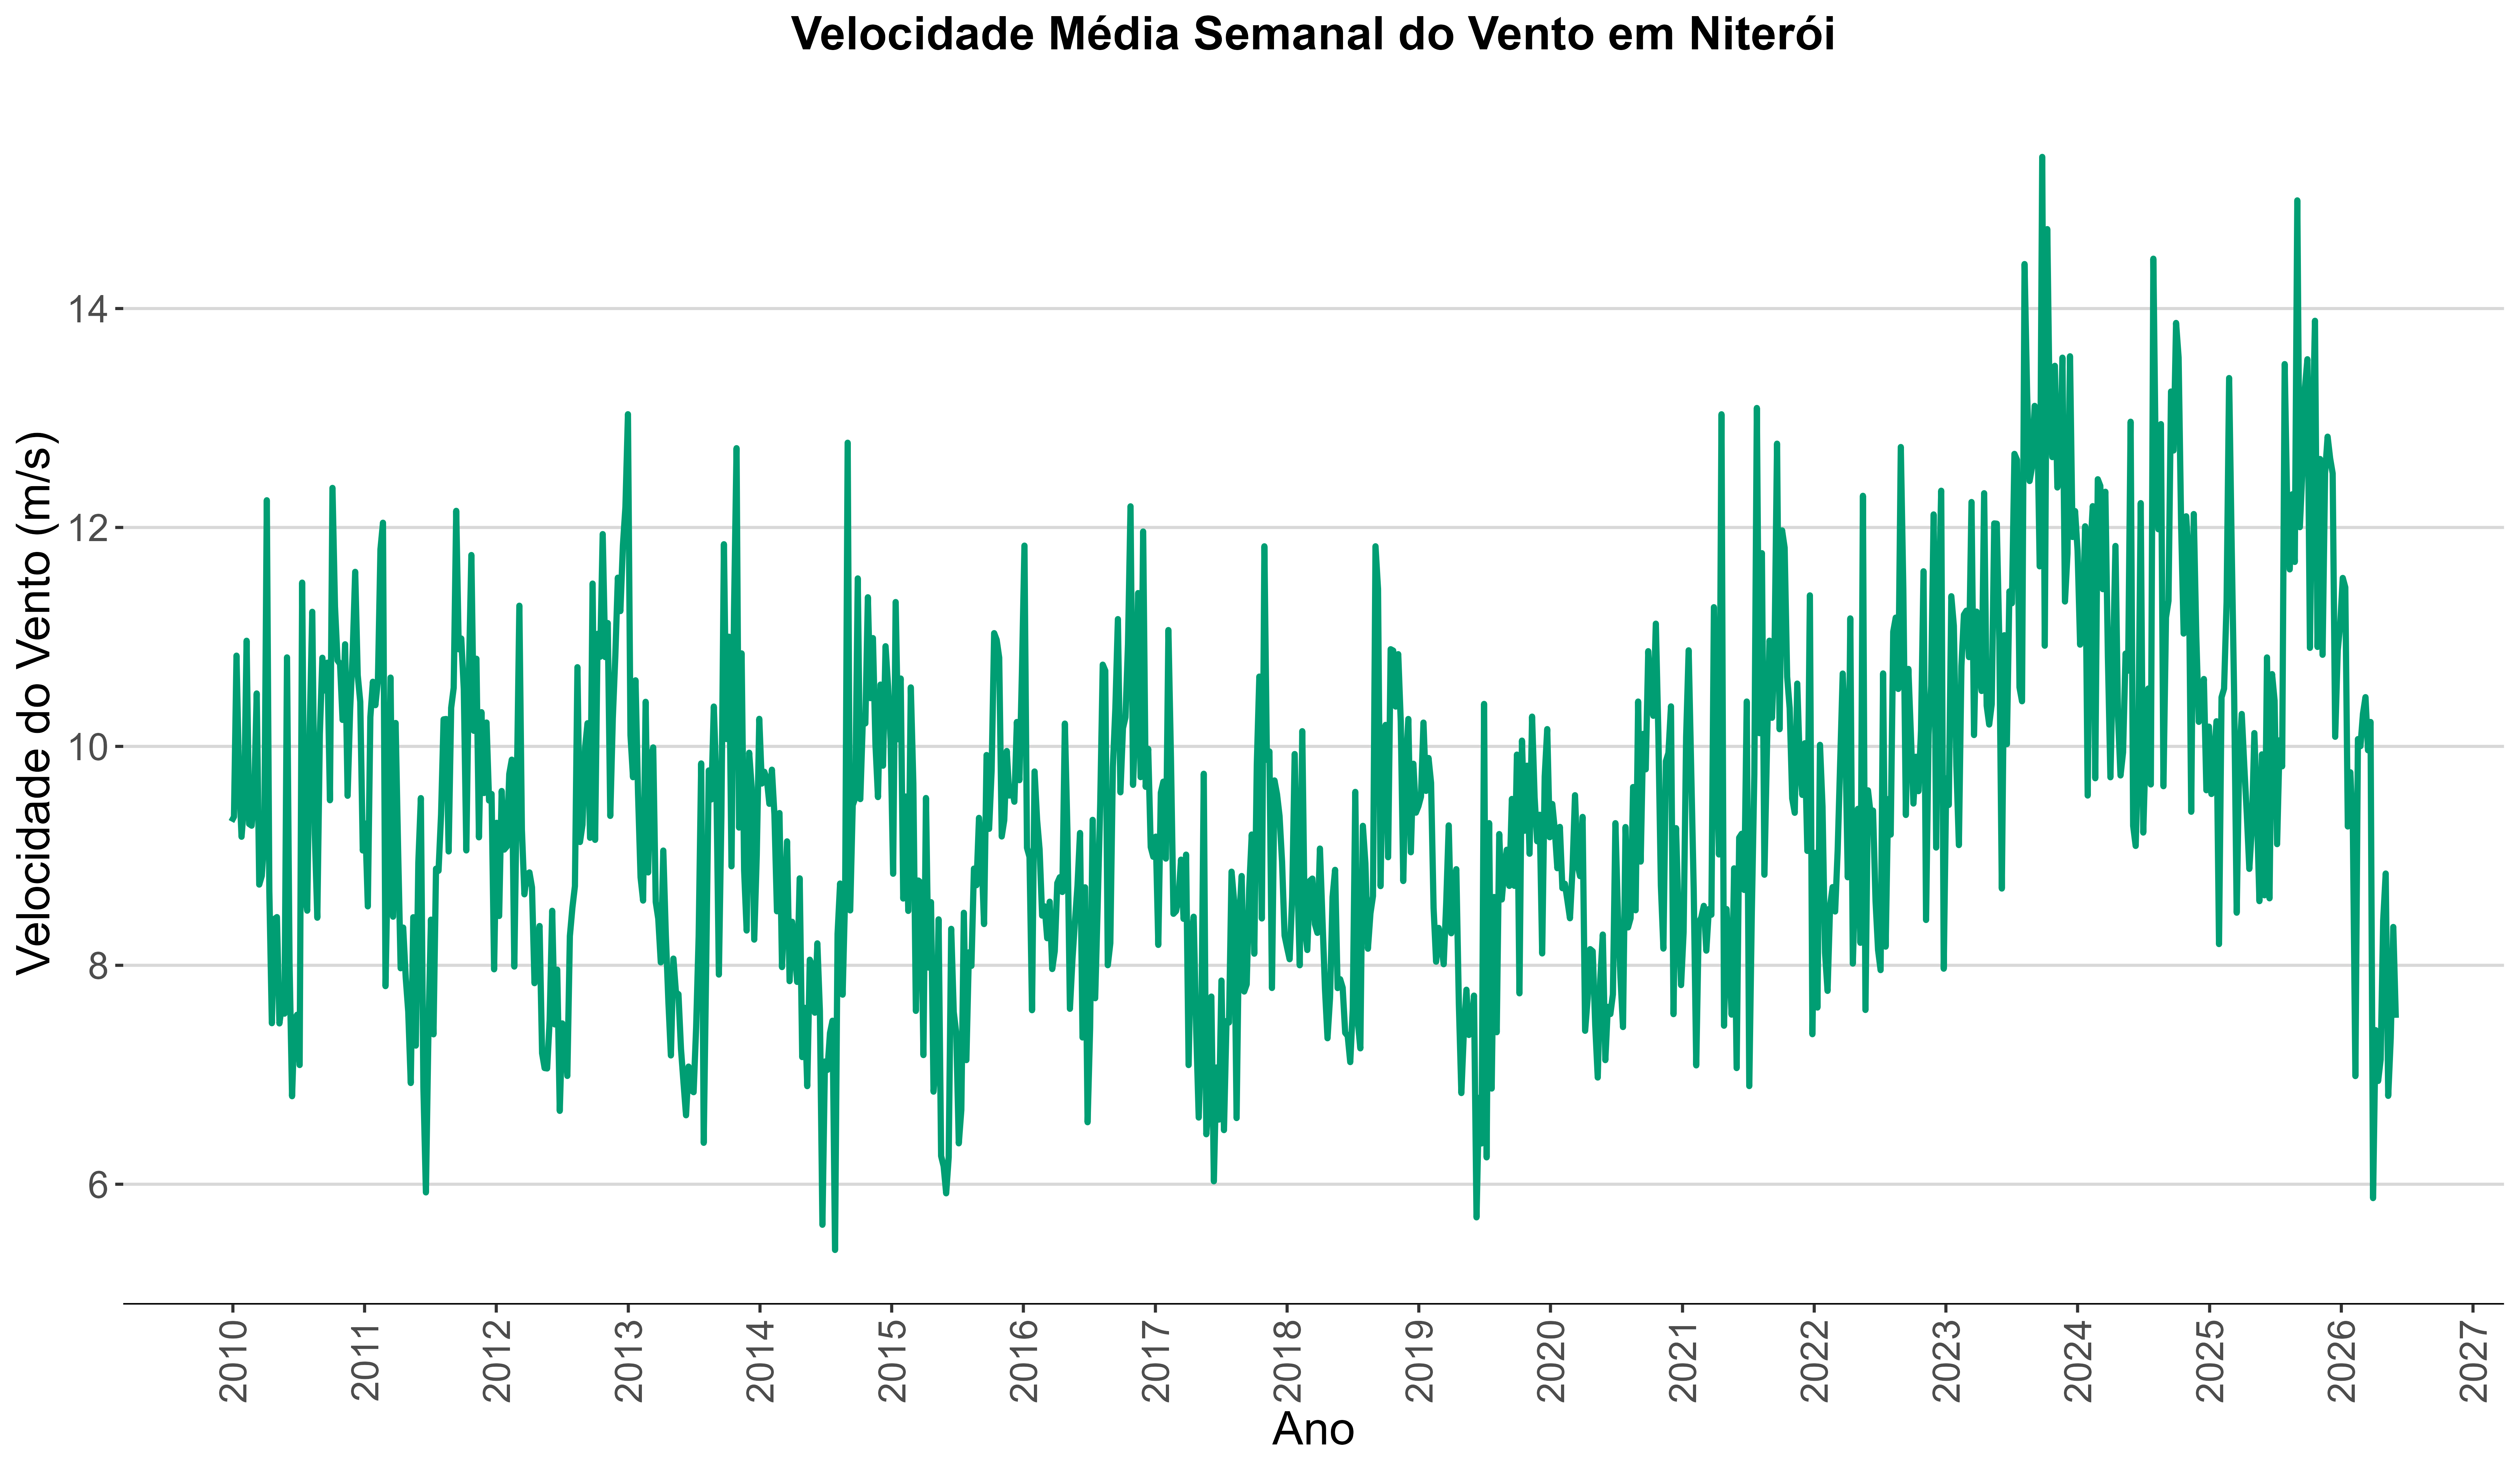
\includegraphics[keepaspectratio]{resultados/VelocVento/02_velocidade_vento_media_semanal.png}}

}

\caption{Velocidade Média Semanal do Vento}

\end{figure}%

\begin{figure}[H]

{\centering \pandocbounded{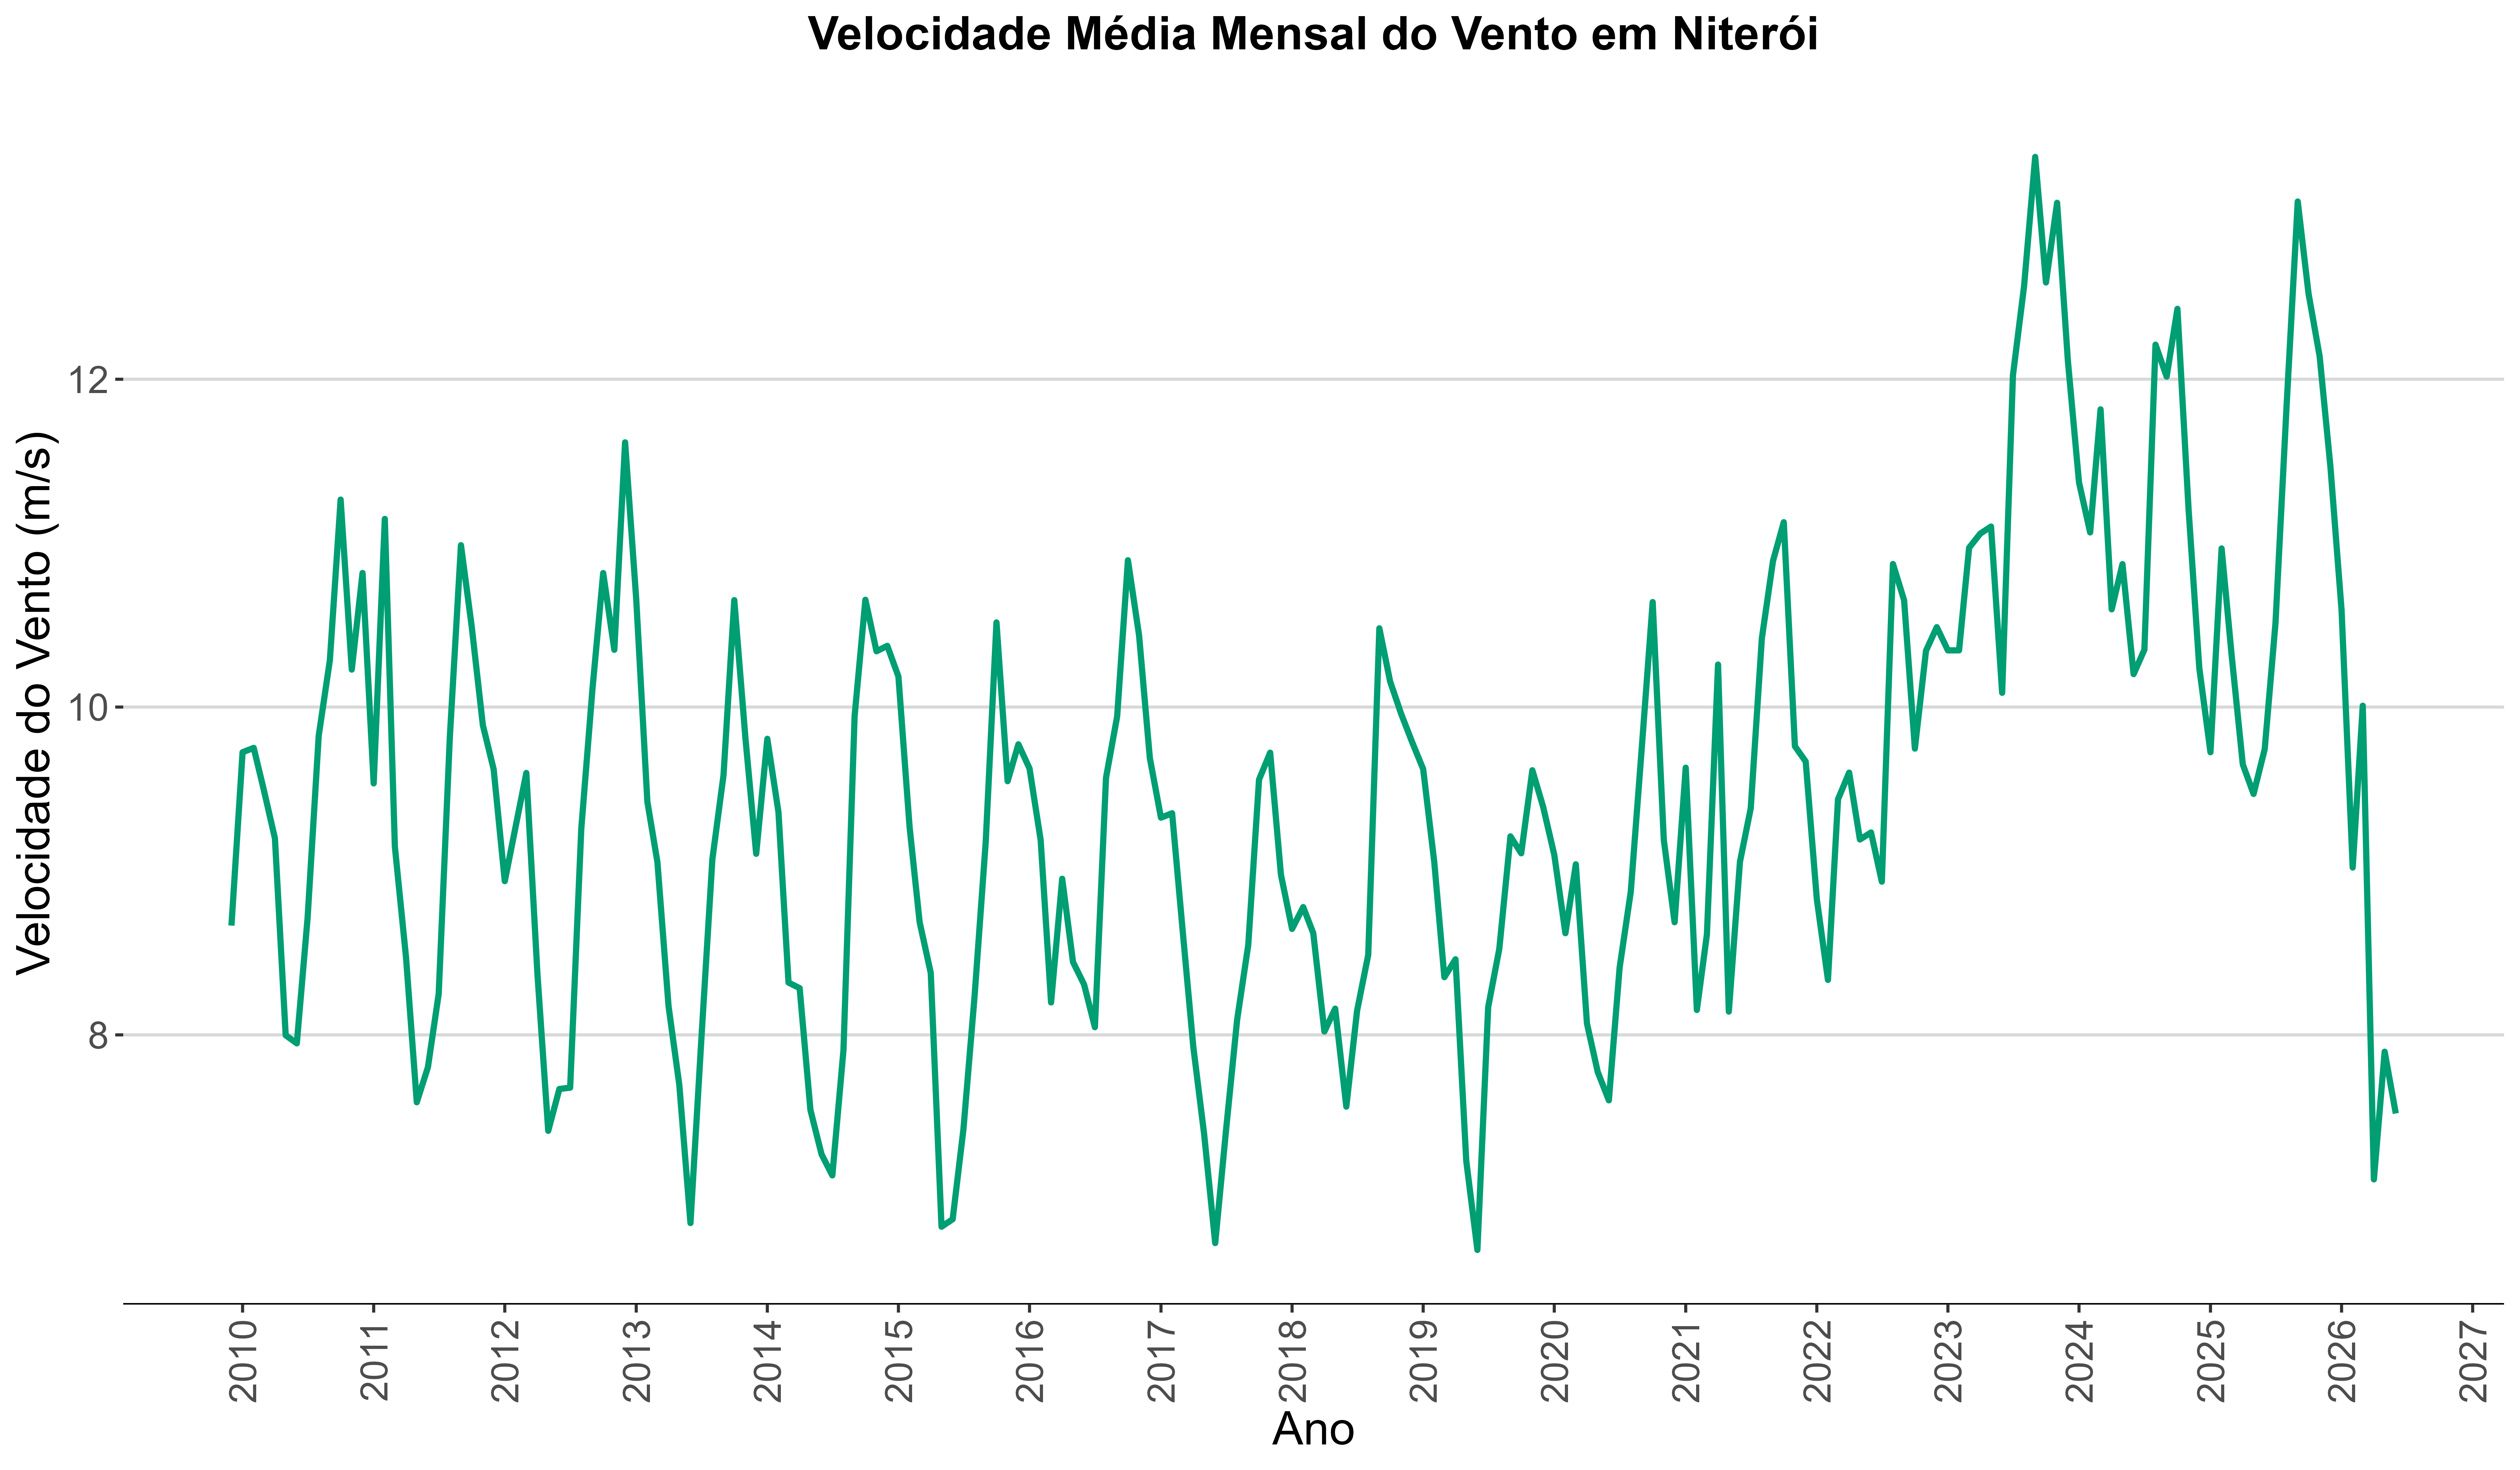
\includegraphics[keepaspectratio]{resultados/VelocVento/03_velocidade_vento_media_mensal.png}}

}

\caption{Velocidade Média Mensal do Vento}

\end{figure}%

\begin{figure}[H]

{\centering \pandocbounded{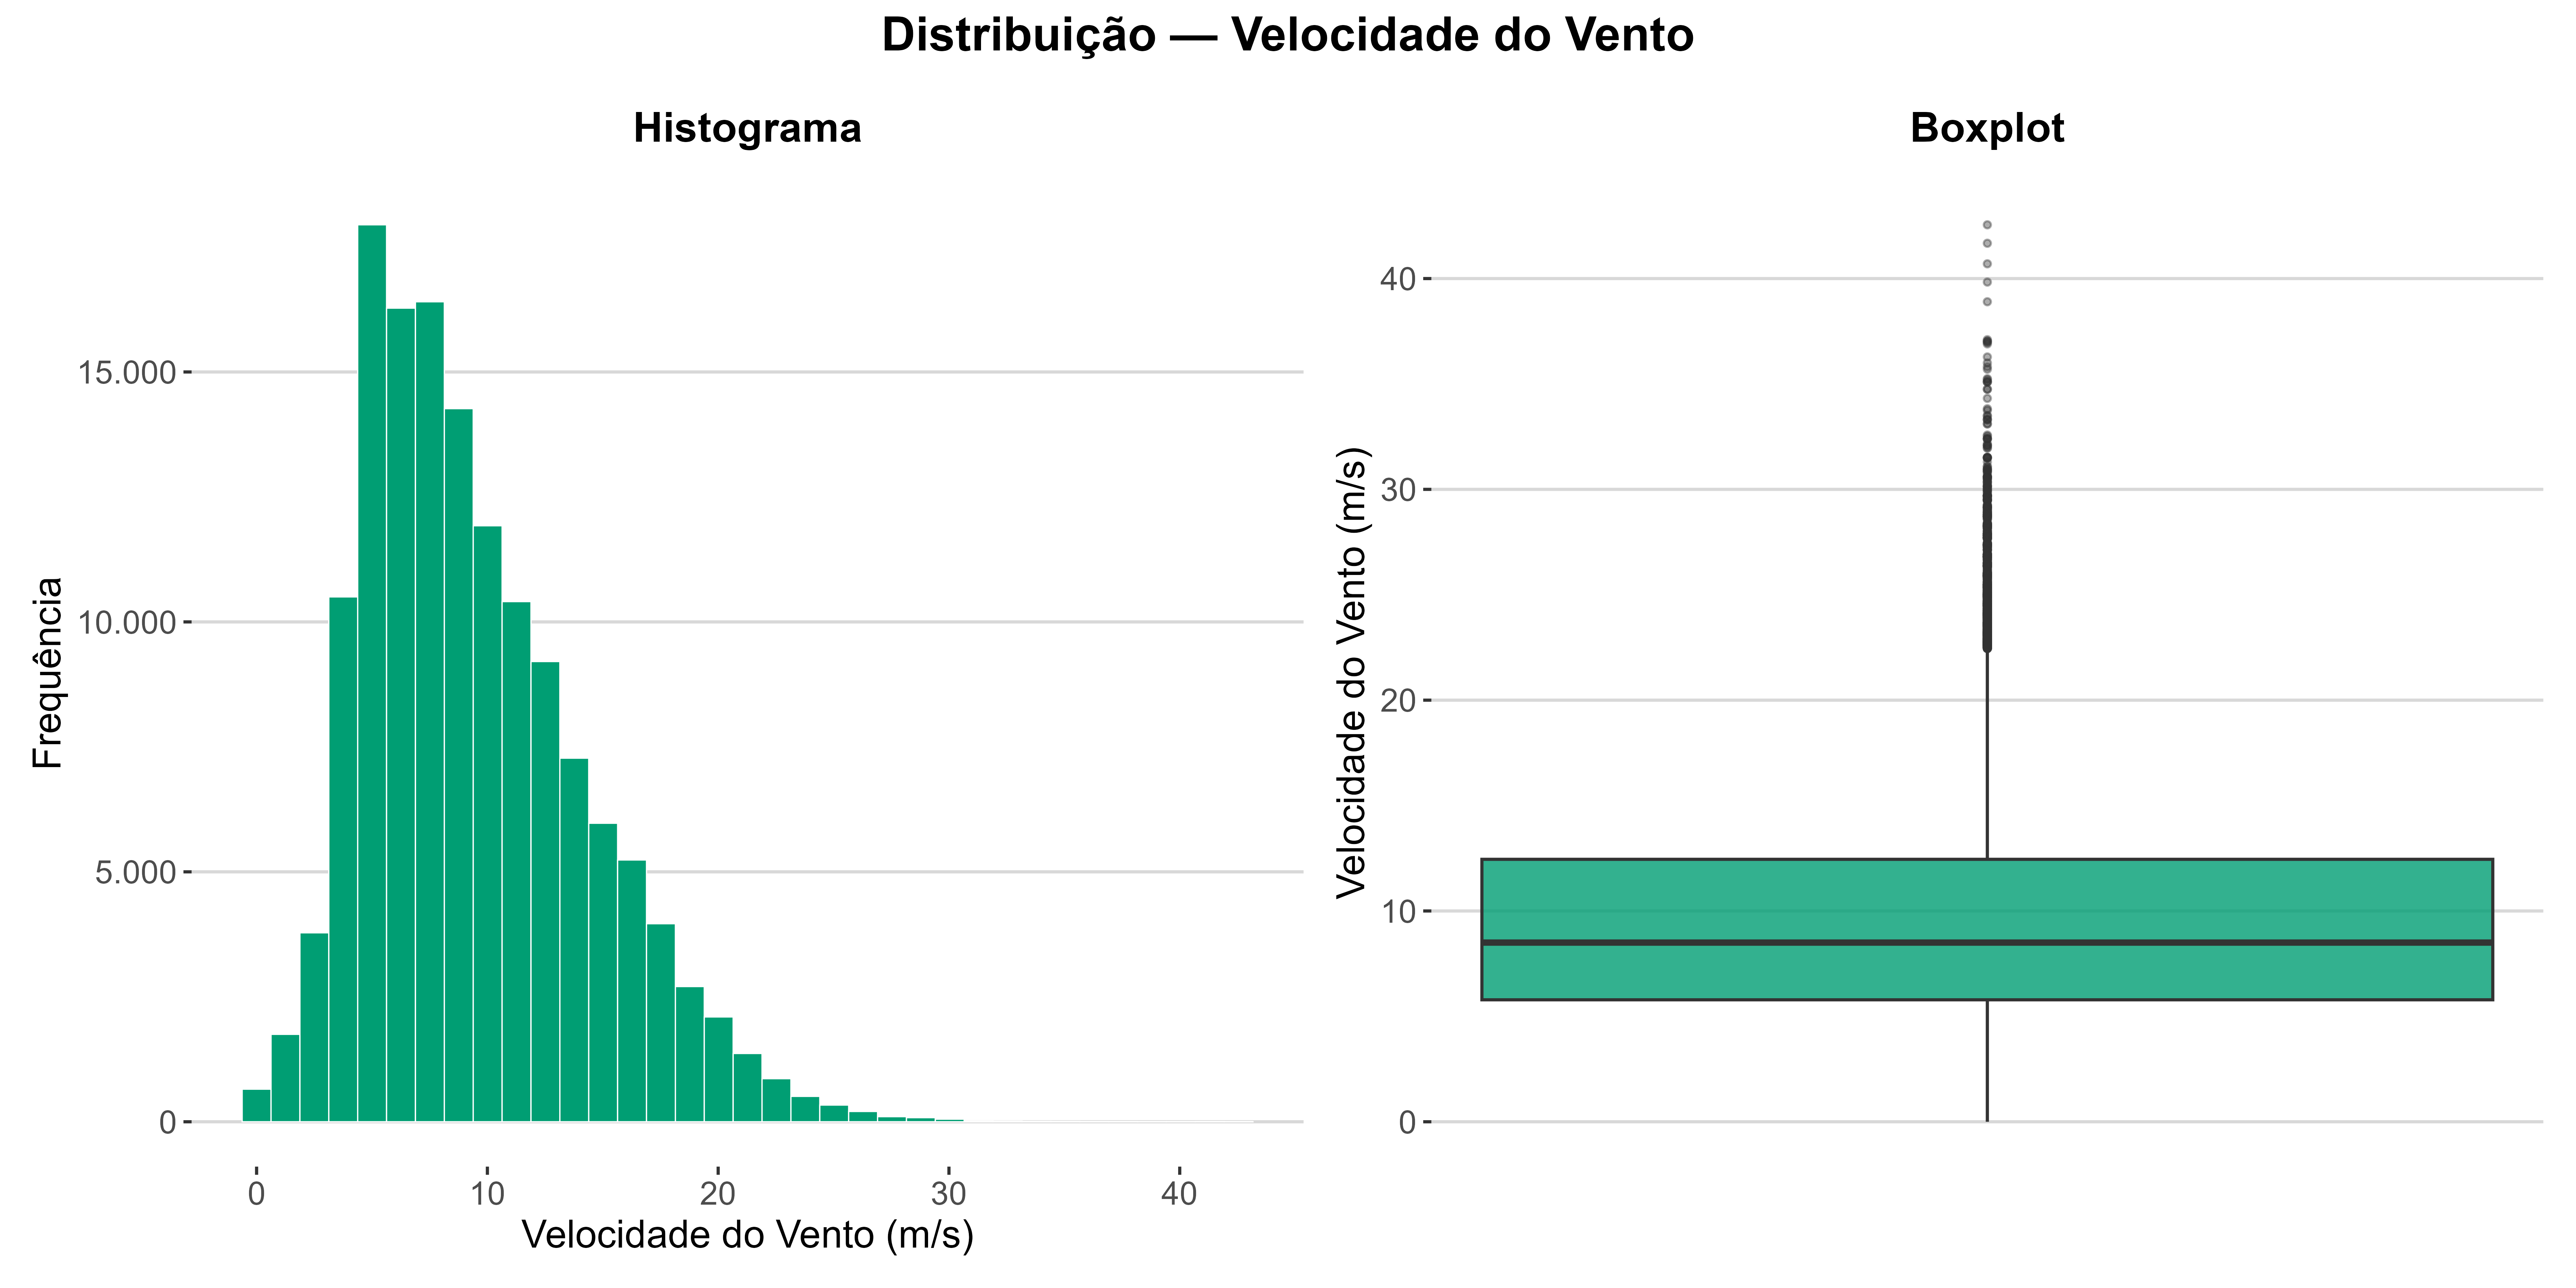
\includegraphics[keepaspectratio]{resultados/VelocVento/04_velocvento_distribuicao.png}}

}

\caption{Distribuição da Velocidade do Vento}

\end{figure}%

\paragraph{Principais Achados}\label{principais-achados-3}

A velocidade do vento horária varia de 0 a cerca de 40 m/s, com a série
apresentando \textbf{alta variabilidade intradiária} e alguns picos
extremos isolados que podem corresponder a eventos convectivos ou
rajadas. A escala diária suaviza esse ruído e revela um padrão de
variação sazonal moderado, com ventos ligeiramente mais intensos no
inverno e primavera.

O histograma mostra distribuição \textbf{assimétrica à direita}, típica
de séries de velocidade de vento, com moda próxima a 5--8 m/s e cauda
estendida. O boxplot evidencia vários outliers superiores, consistentes
com os picos observados na série horária.

\subsubsection{Temperatura da
Superfície}\label{temperatura-da-superfuxedcie}

\begin{figure}[H]

{\centering \pandocbounded{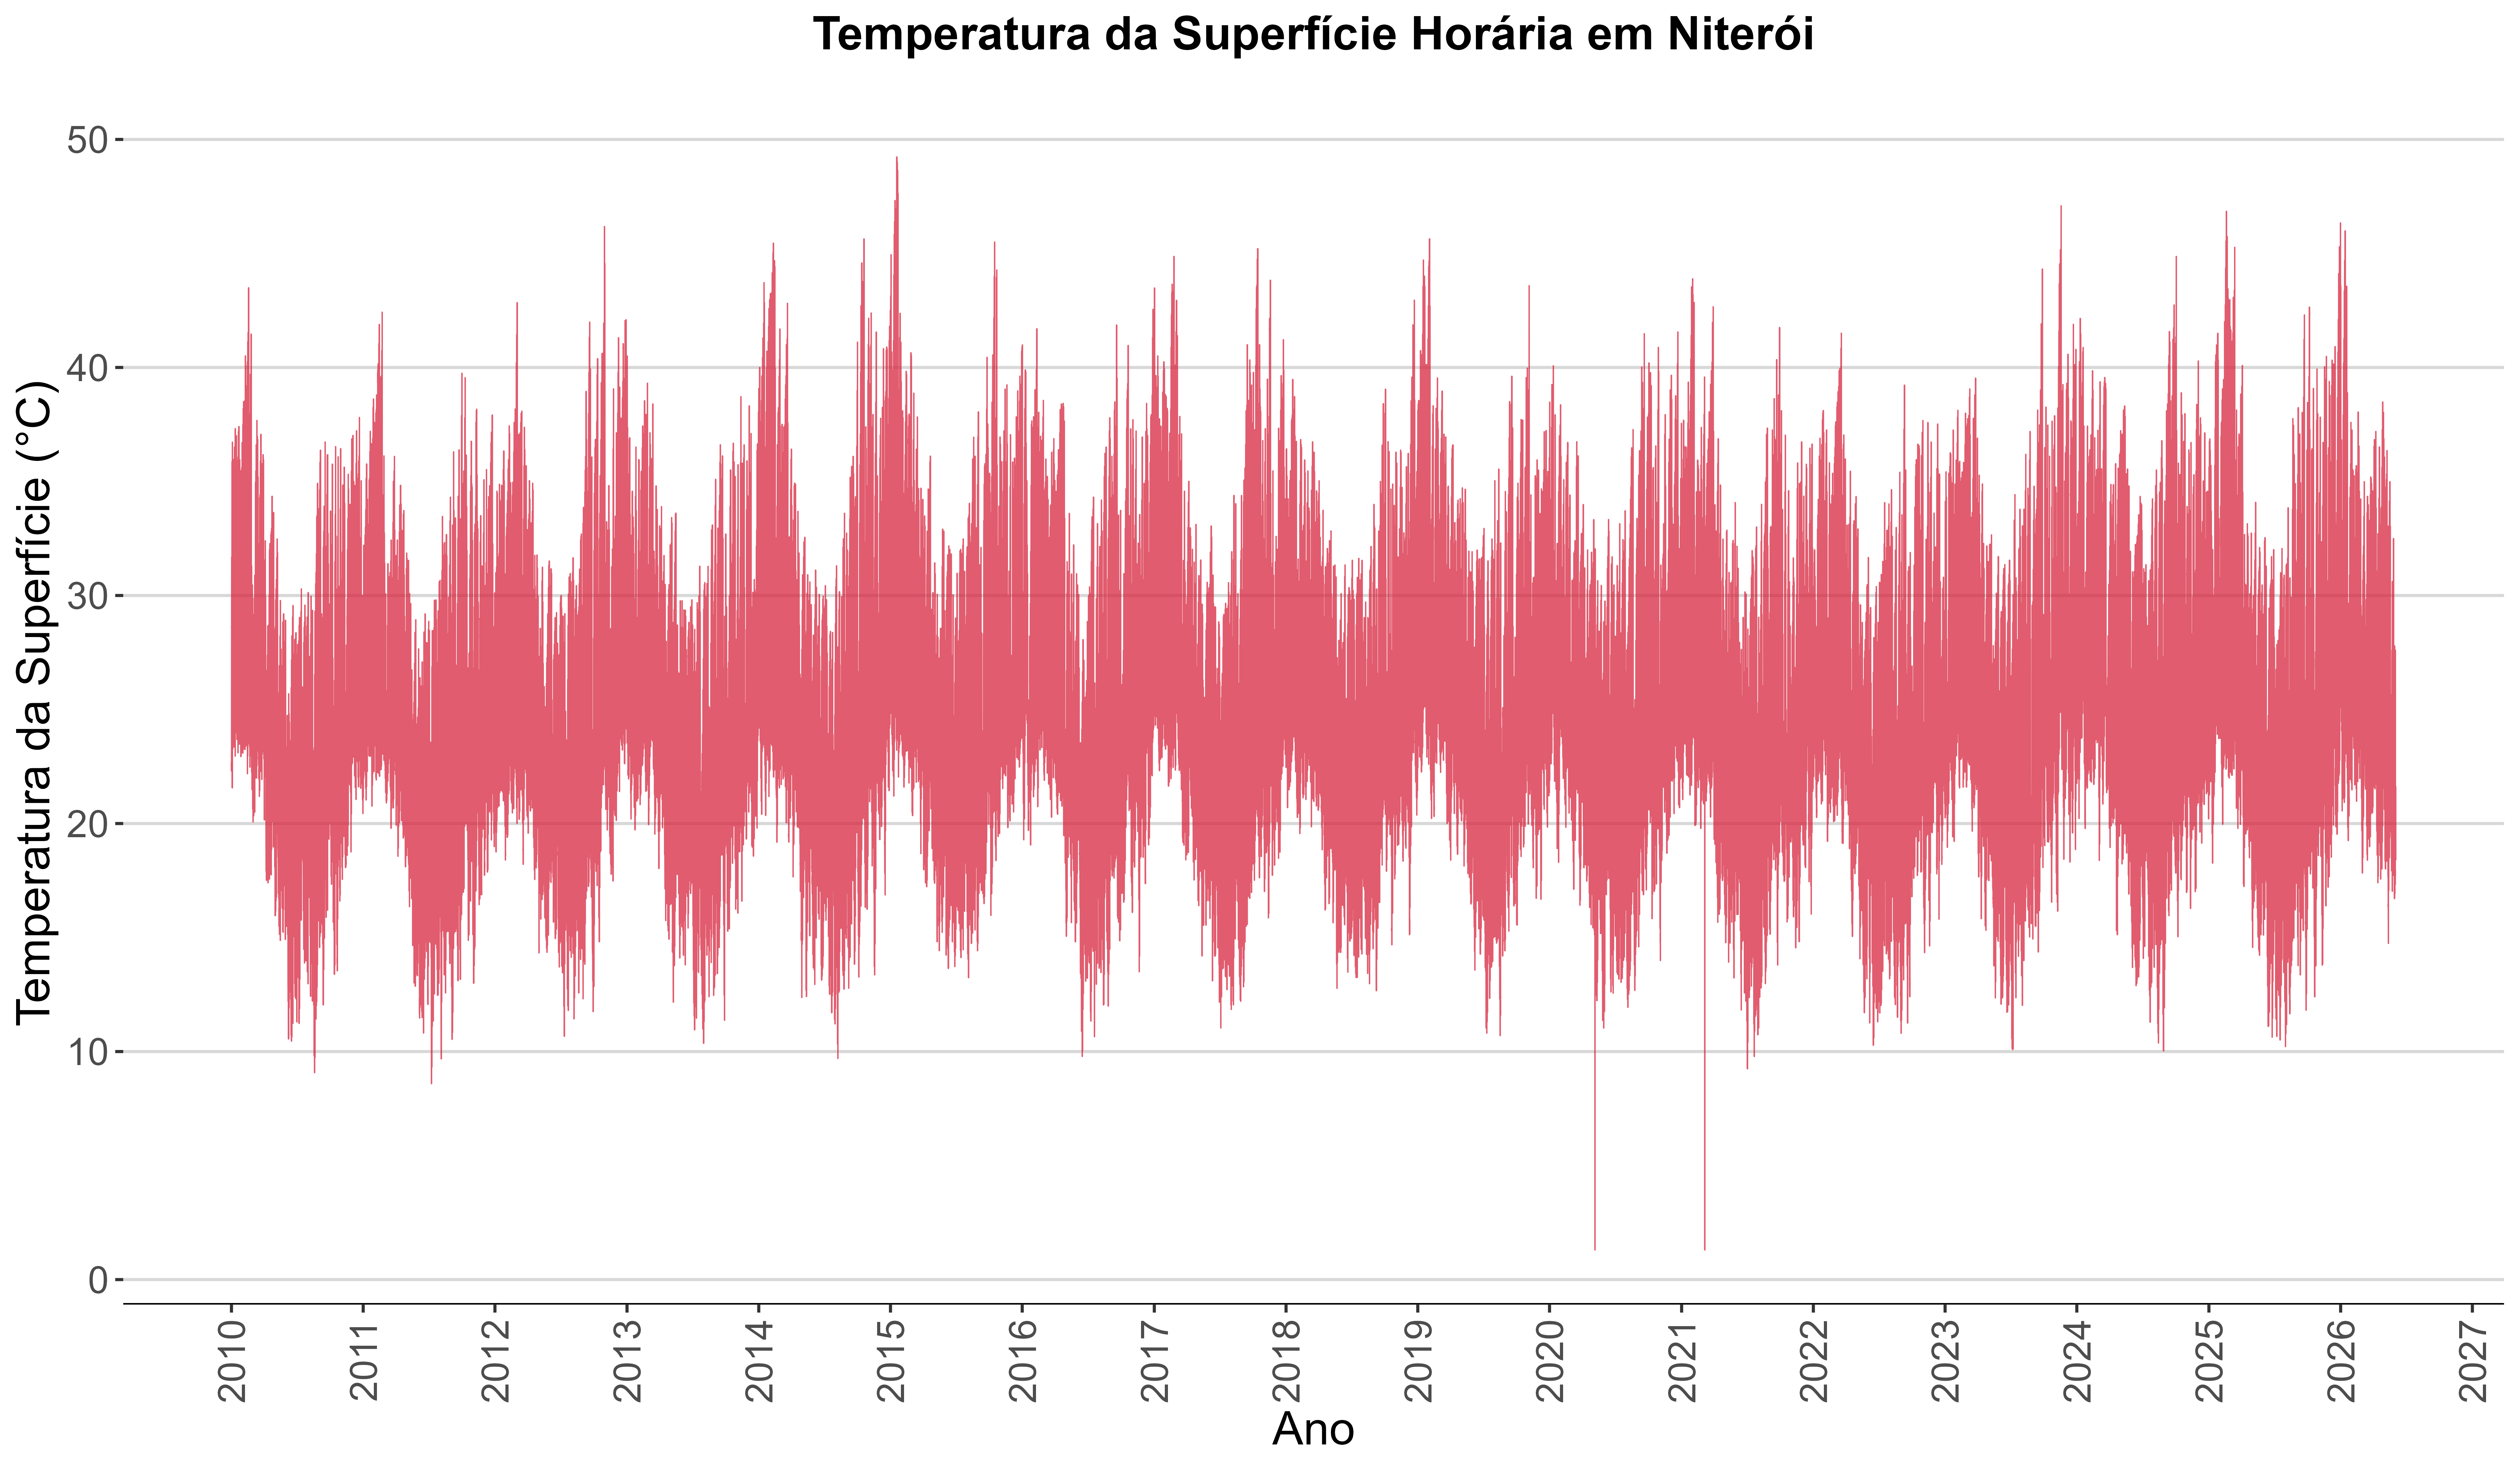
\includegraphics[keepaspectratio]{resultados/TempSuperficie/00_tempsuperficie_horario.png}}

}

\caption{Temperatura da Superfície Horária}

\end{figure}%

\begin{figure}[H]

{\centering \pandocbounded{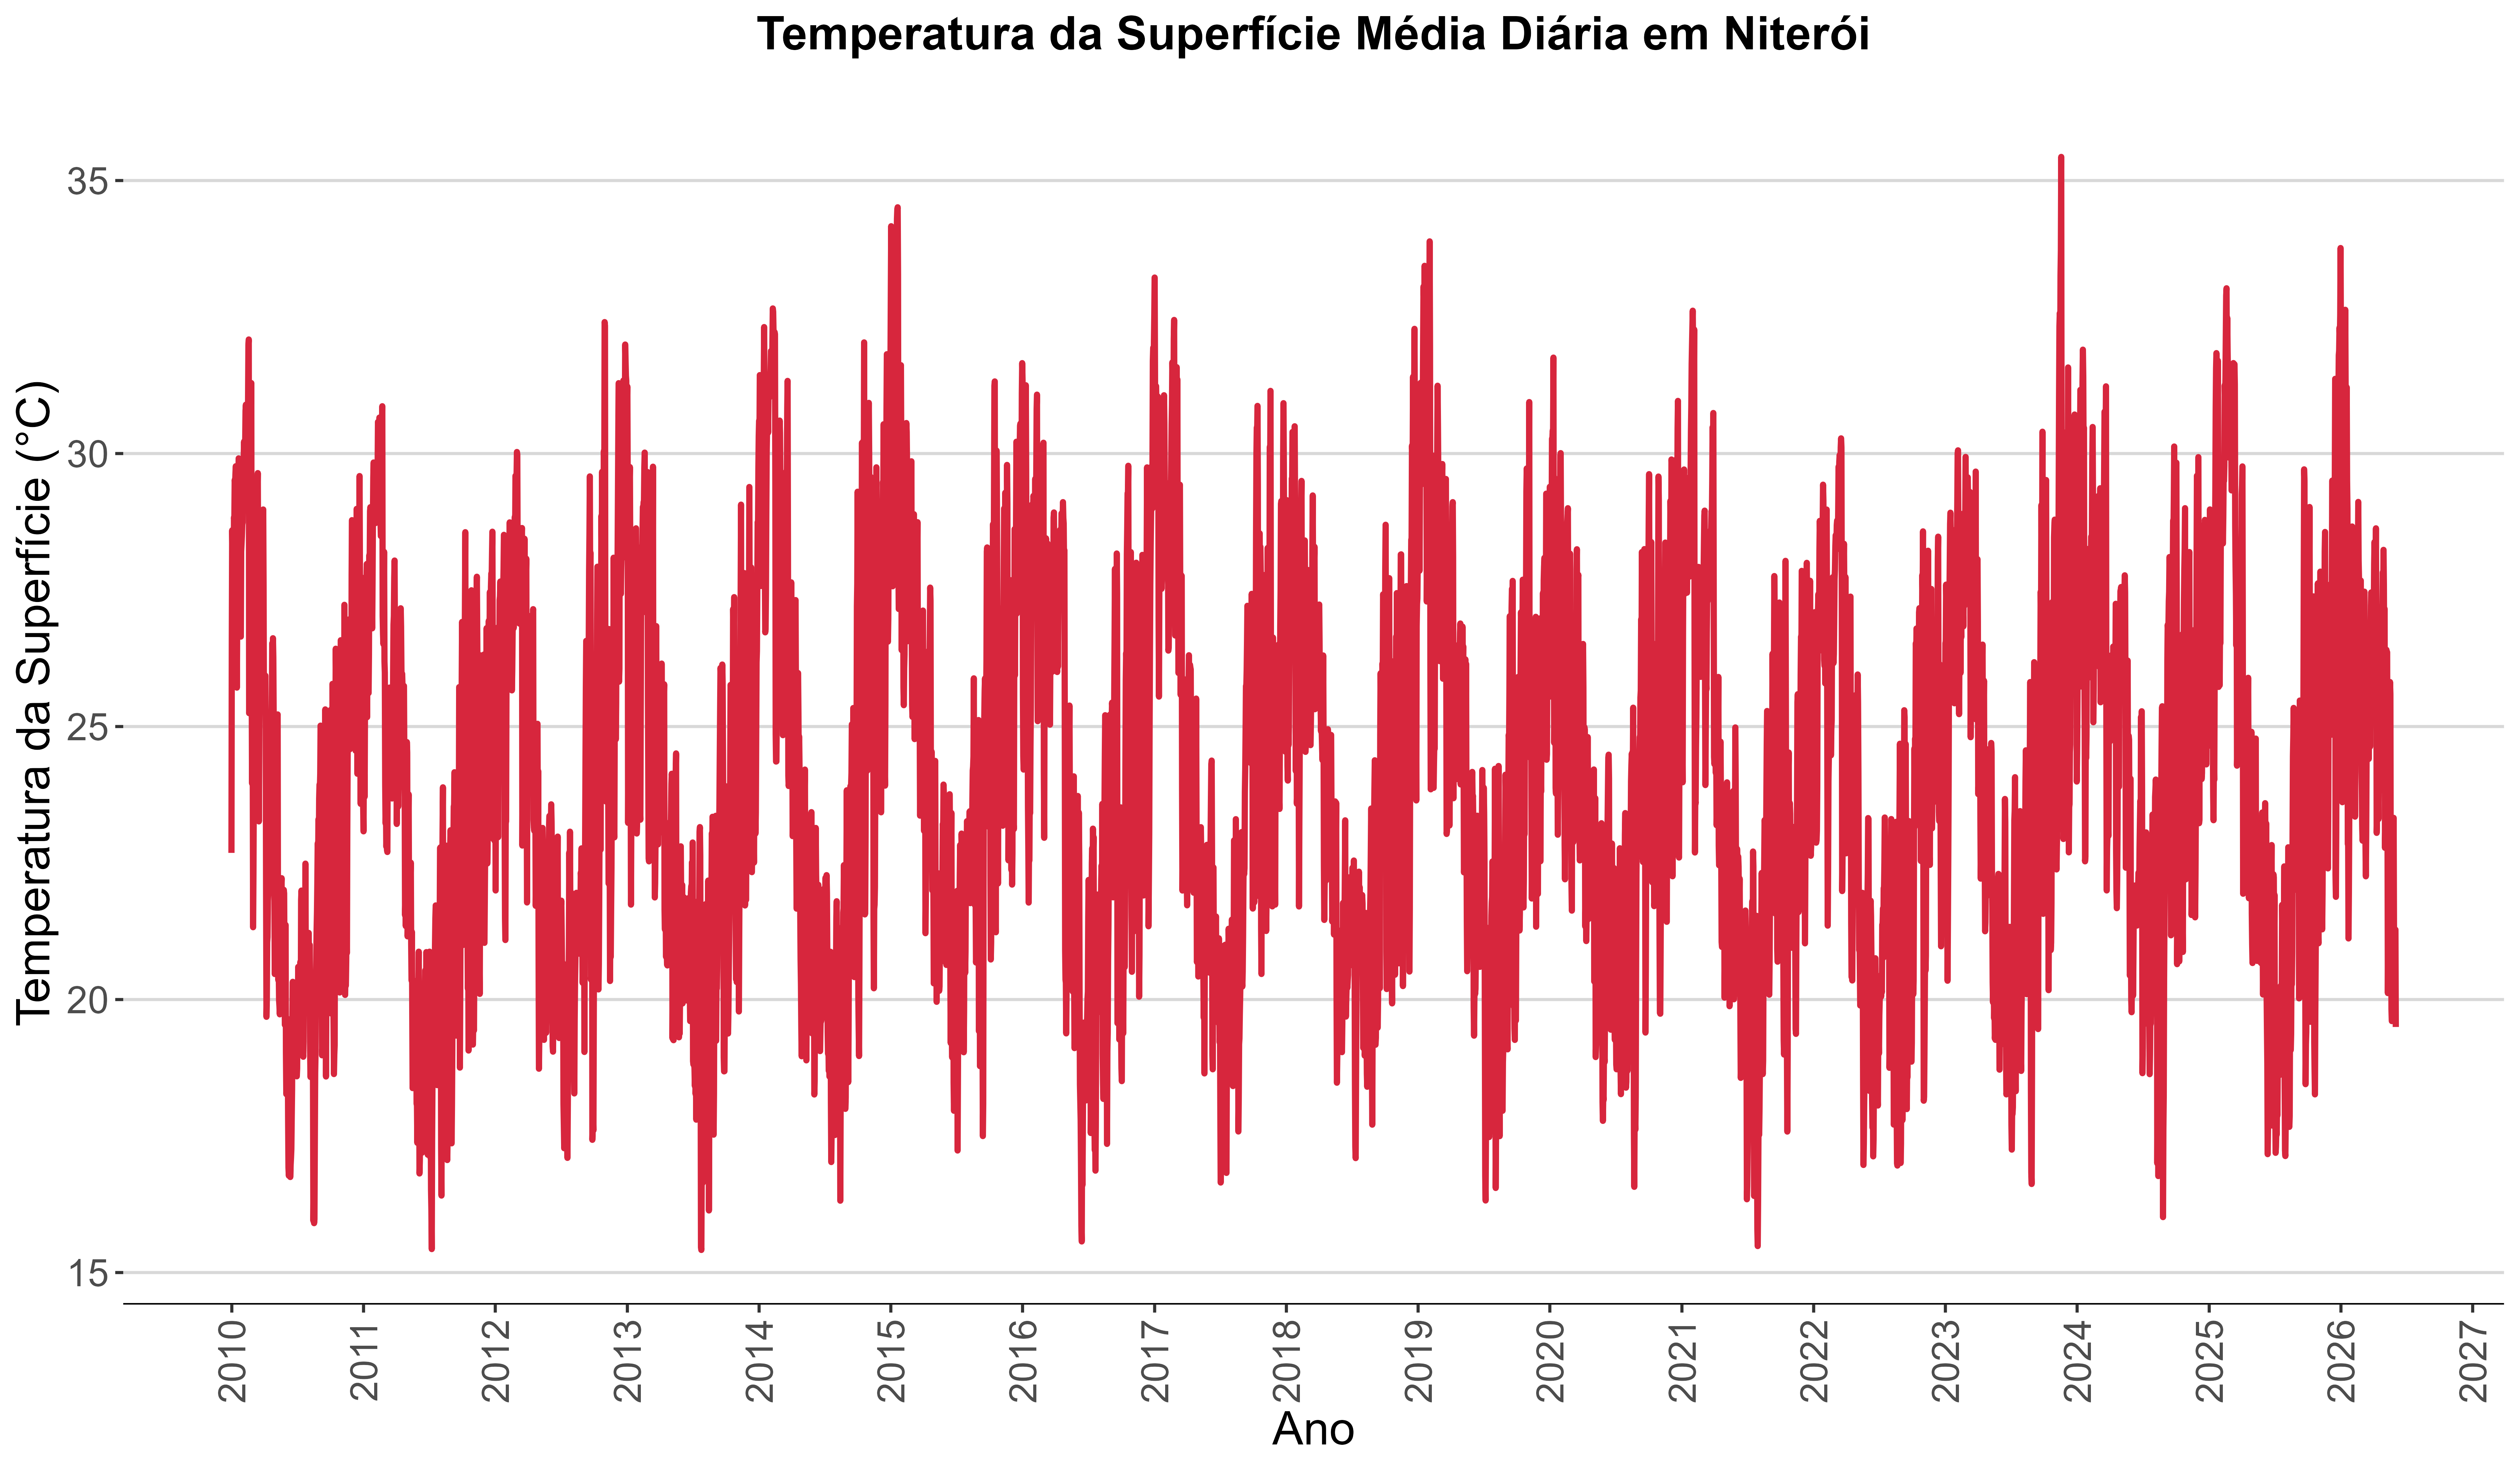
\includegraphics[keepaspectratio]{resultados/TempSuperficie/01_tempsuperficie_diario.png}}

}

\caption{Temperatura da Superfície Média Diária}

\end{figure}%

\begin{figure}[H]

{\centering \pandocbounded{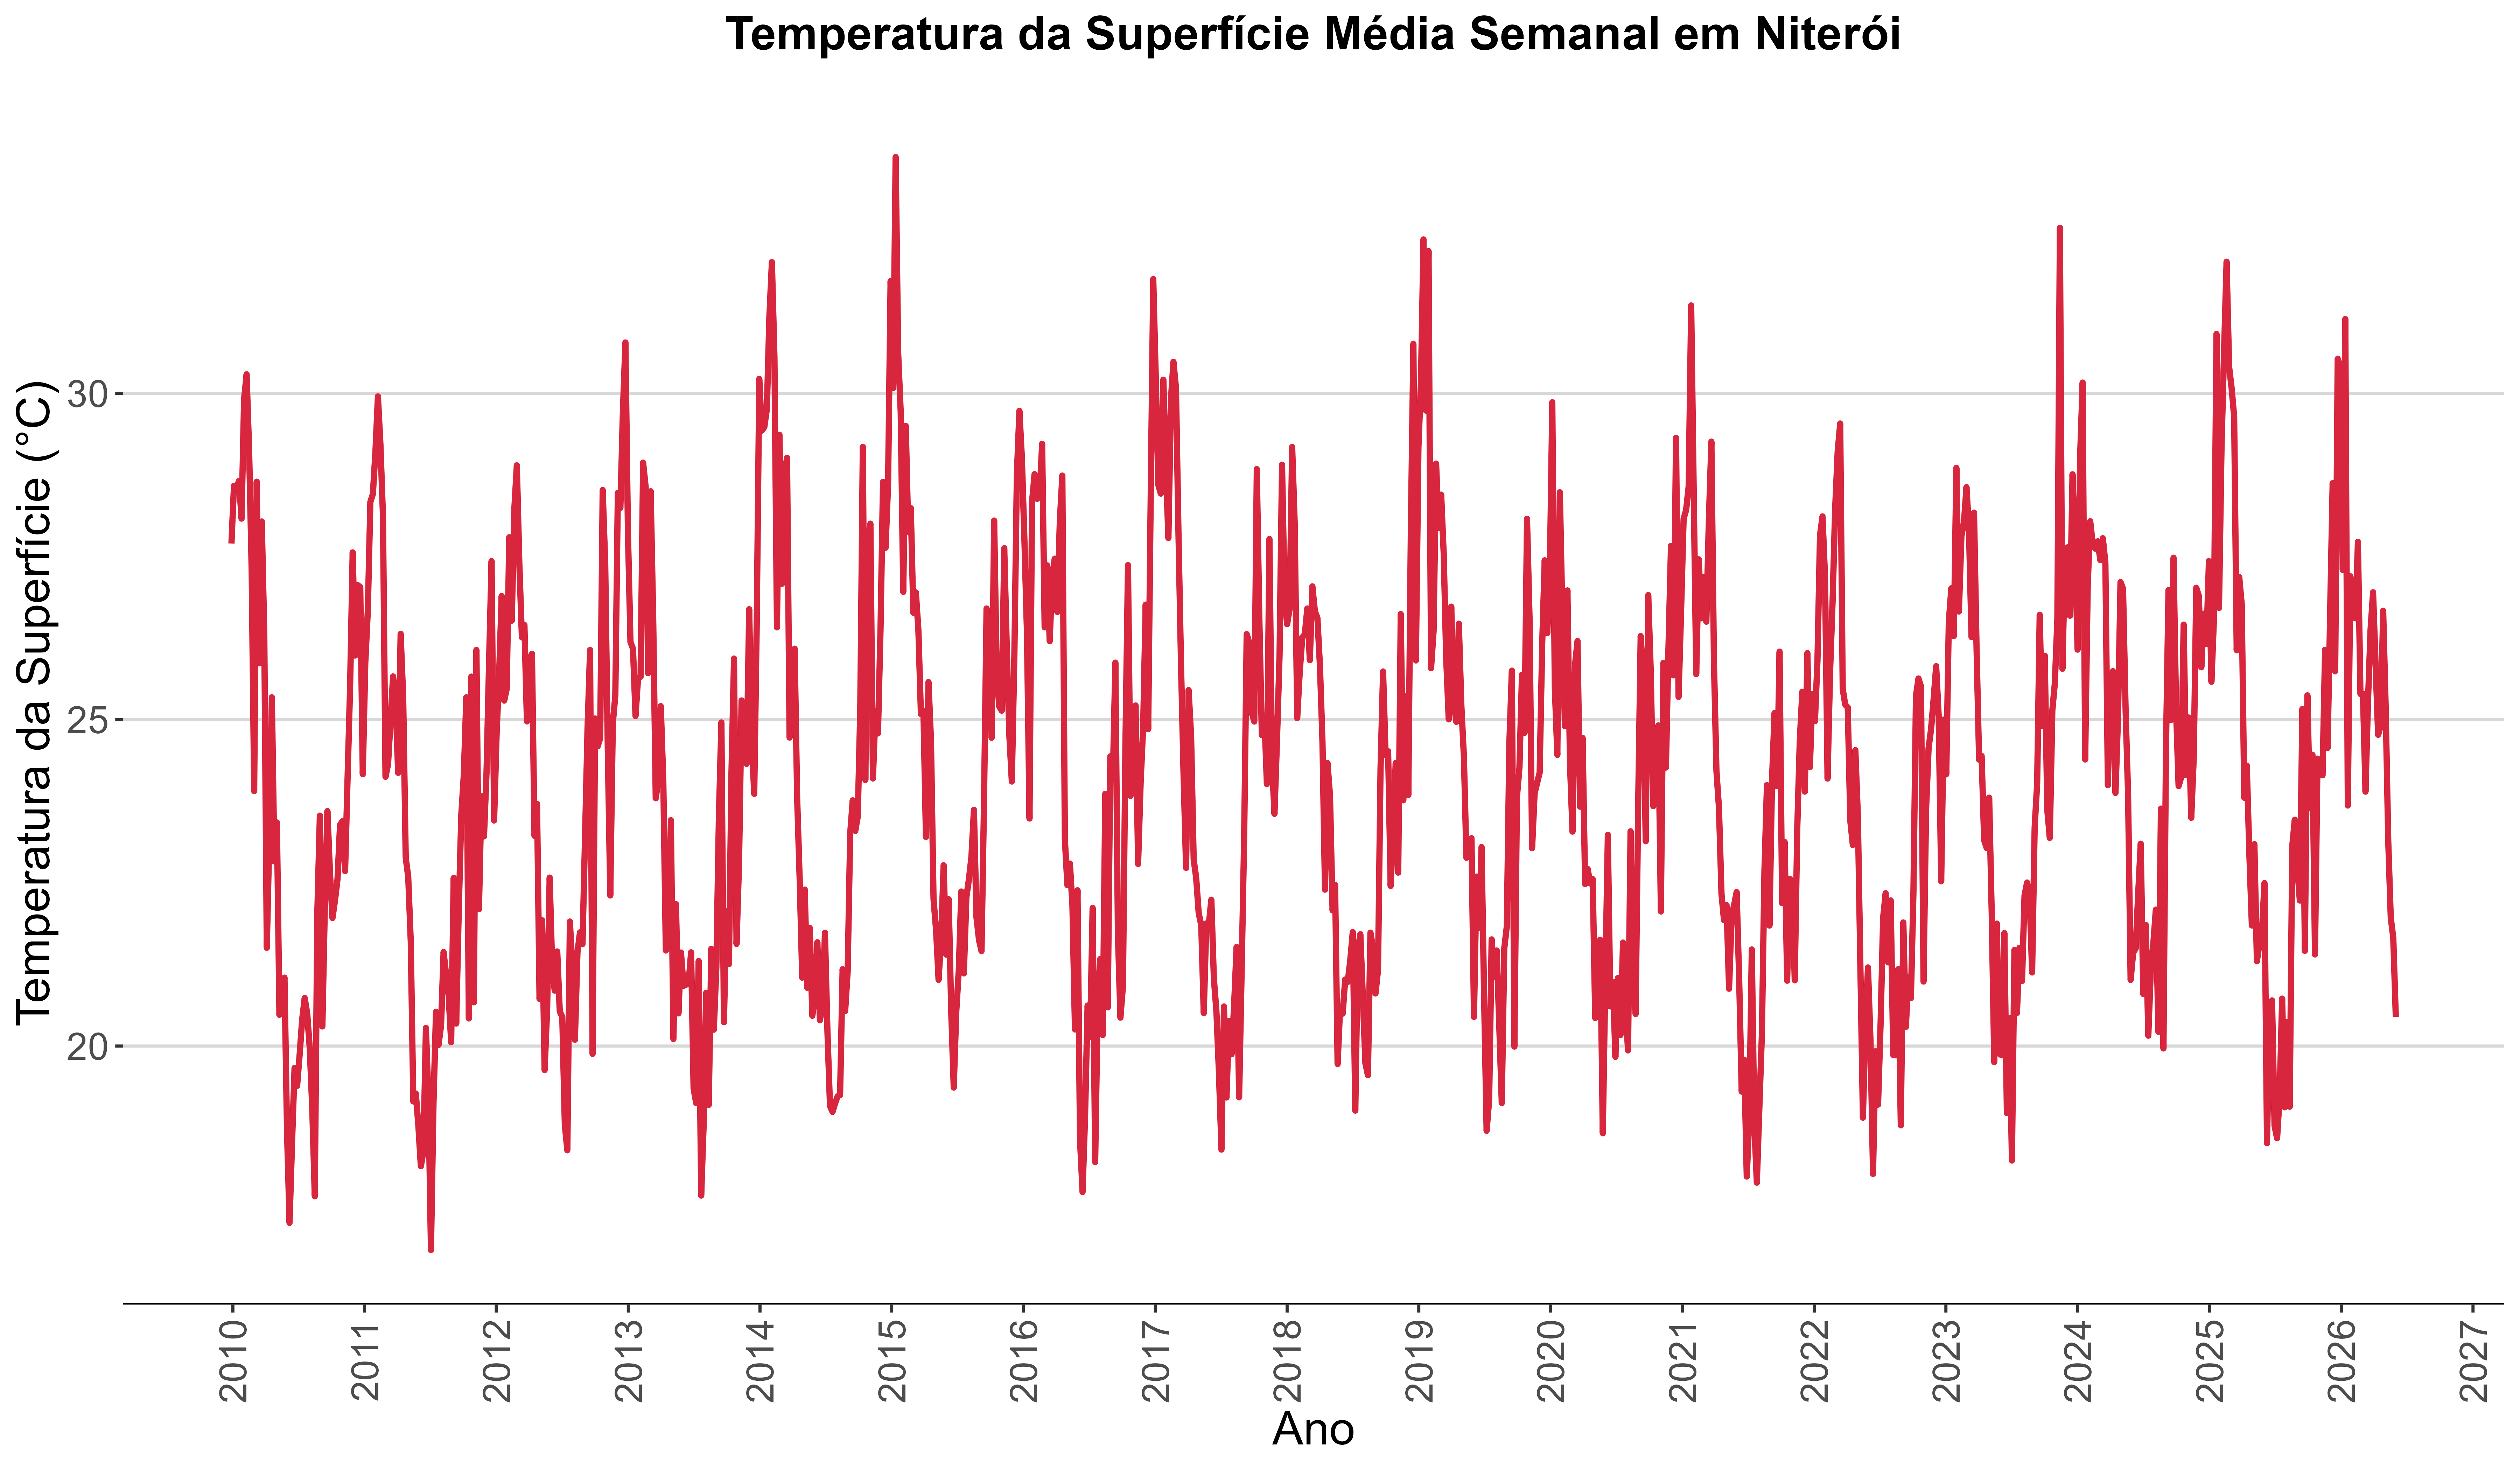
\includegraphics[keepaspectratio]{resultados/TempSuperficie/02_tempsuperficie_semanal.png}}

}

\caption{Temperatura da Superfície Média Semanal}

\end{figure}%

\begin{figure}[H]

{\centering \pandocbounded{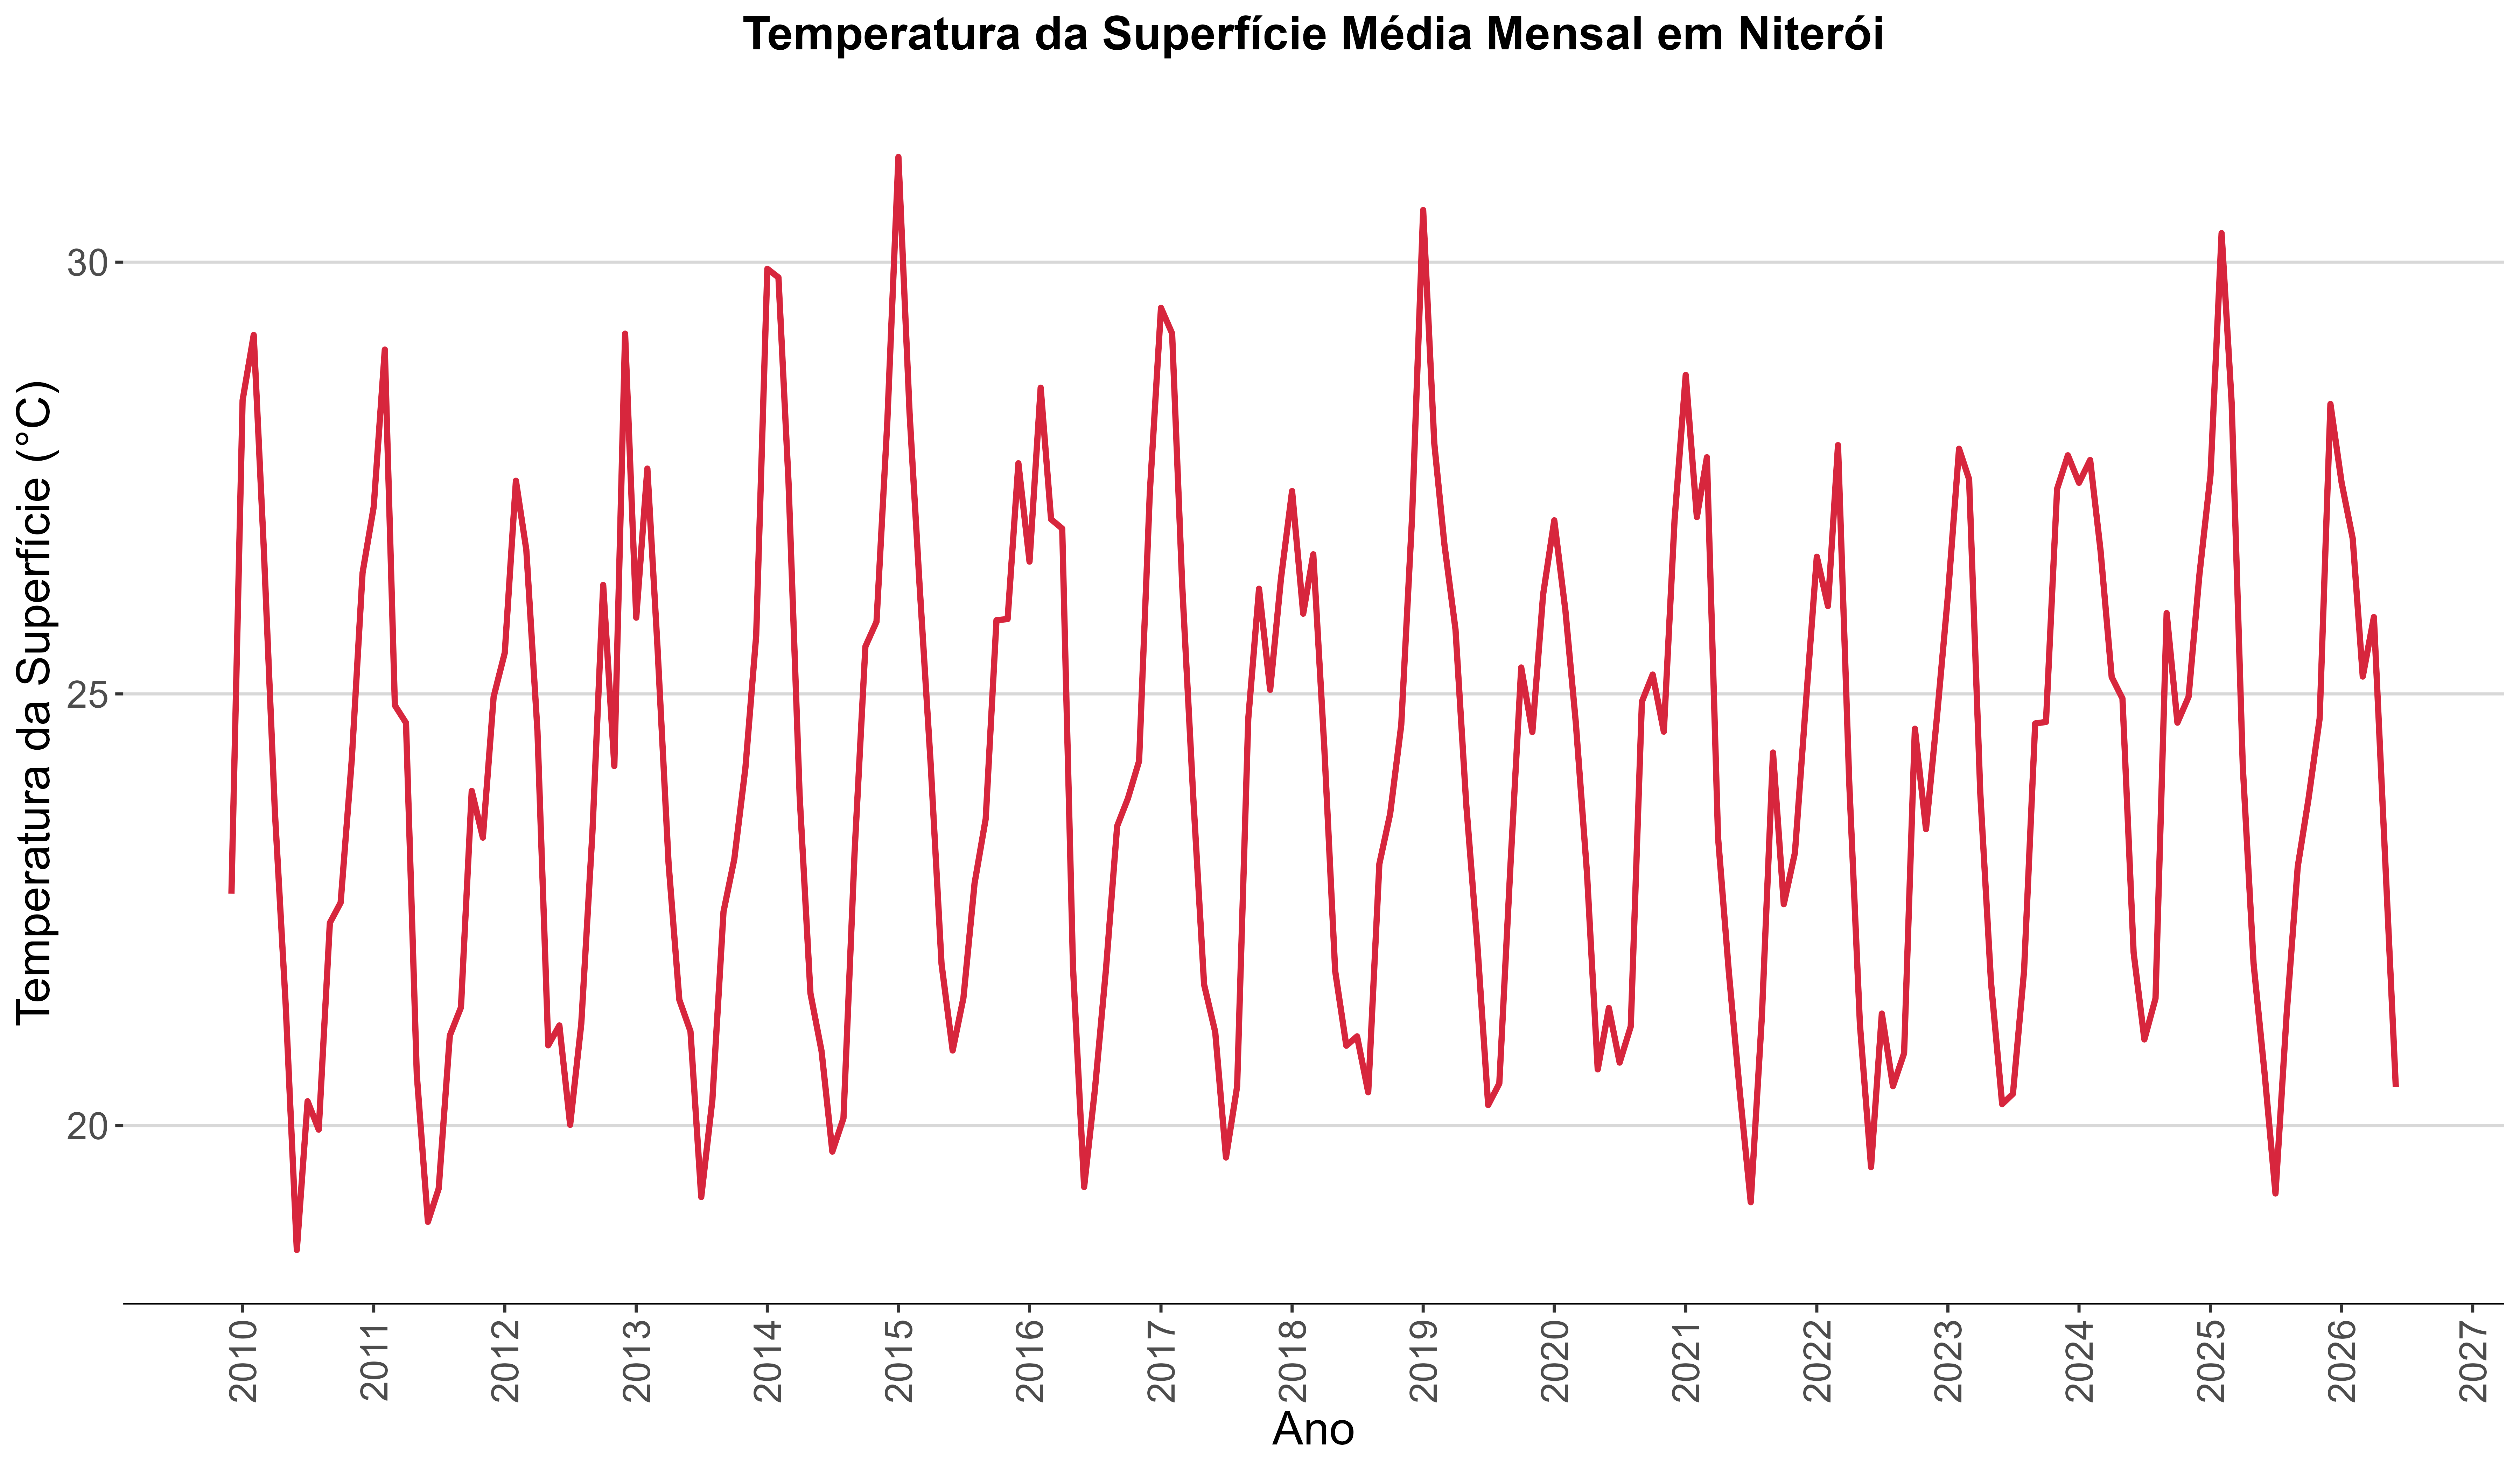
\includegraphics[keepaspectratio]{resultados/TempSuperficie/03_tempsuperficie_mensal.png}}

}

\caption{Temperatura da Superfície Média Mensal}

\end{figure}%

\begin{figure}[H]

{\centering \pandocbounded{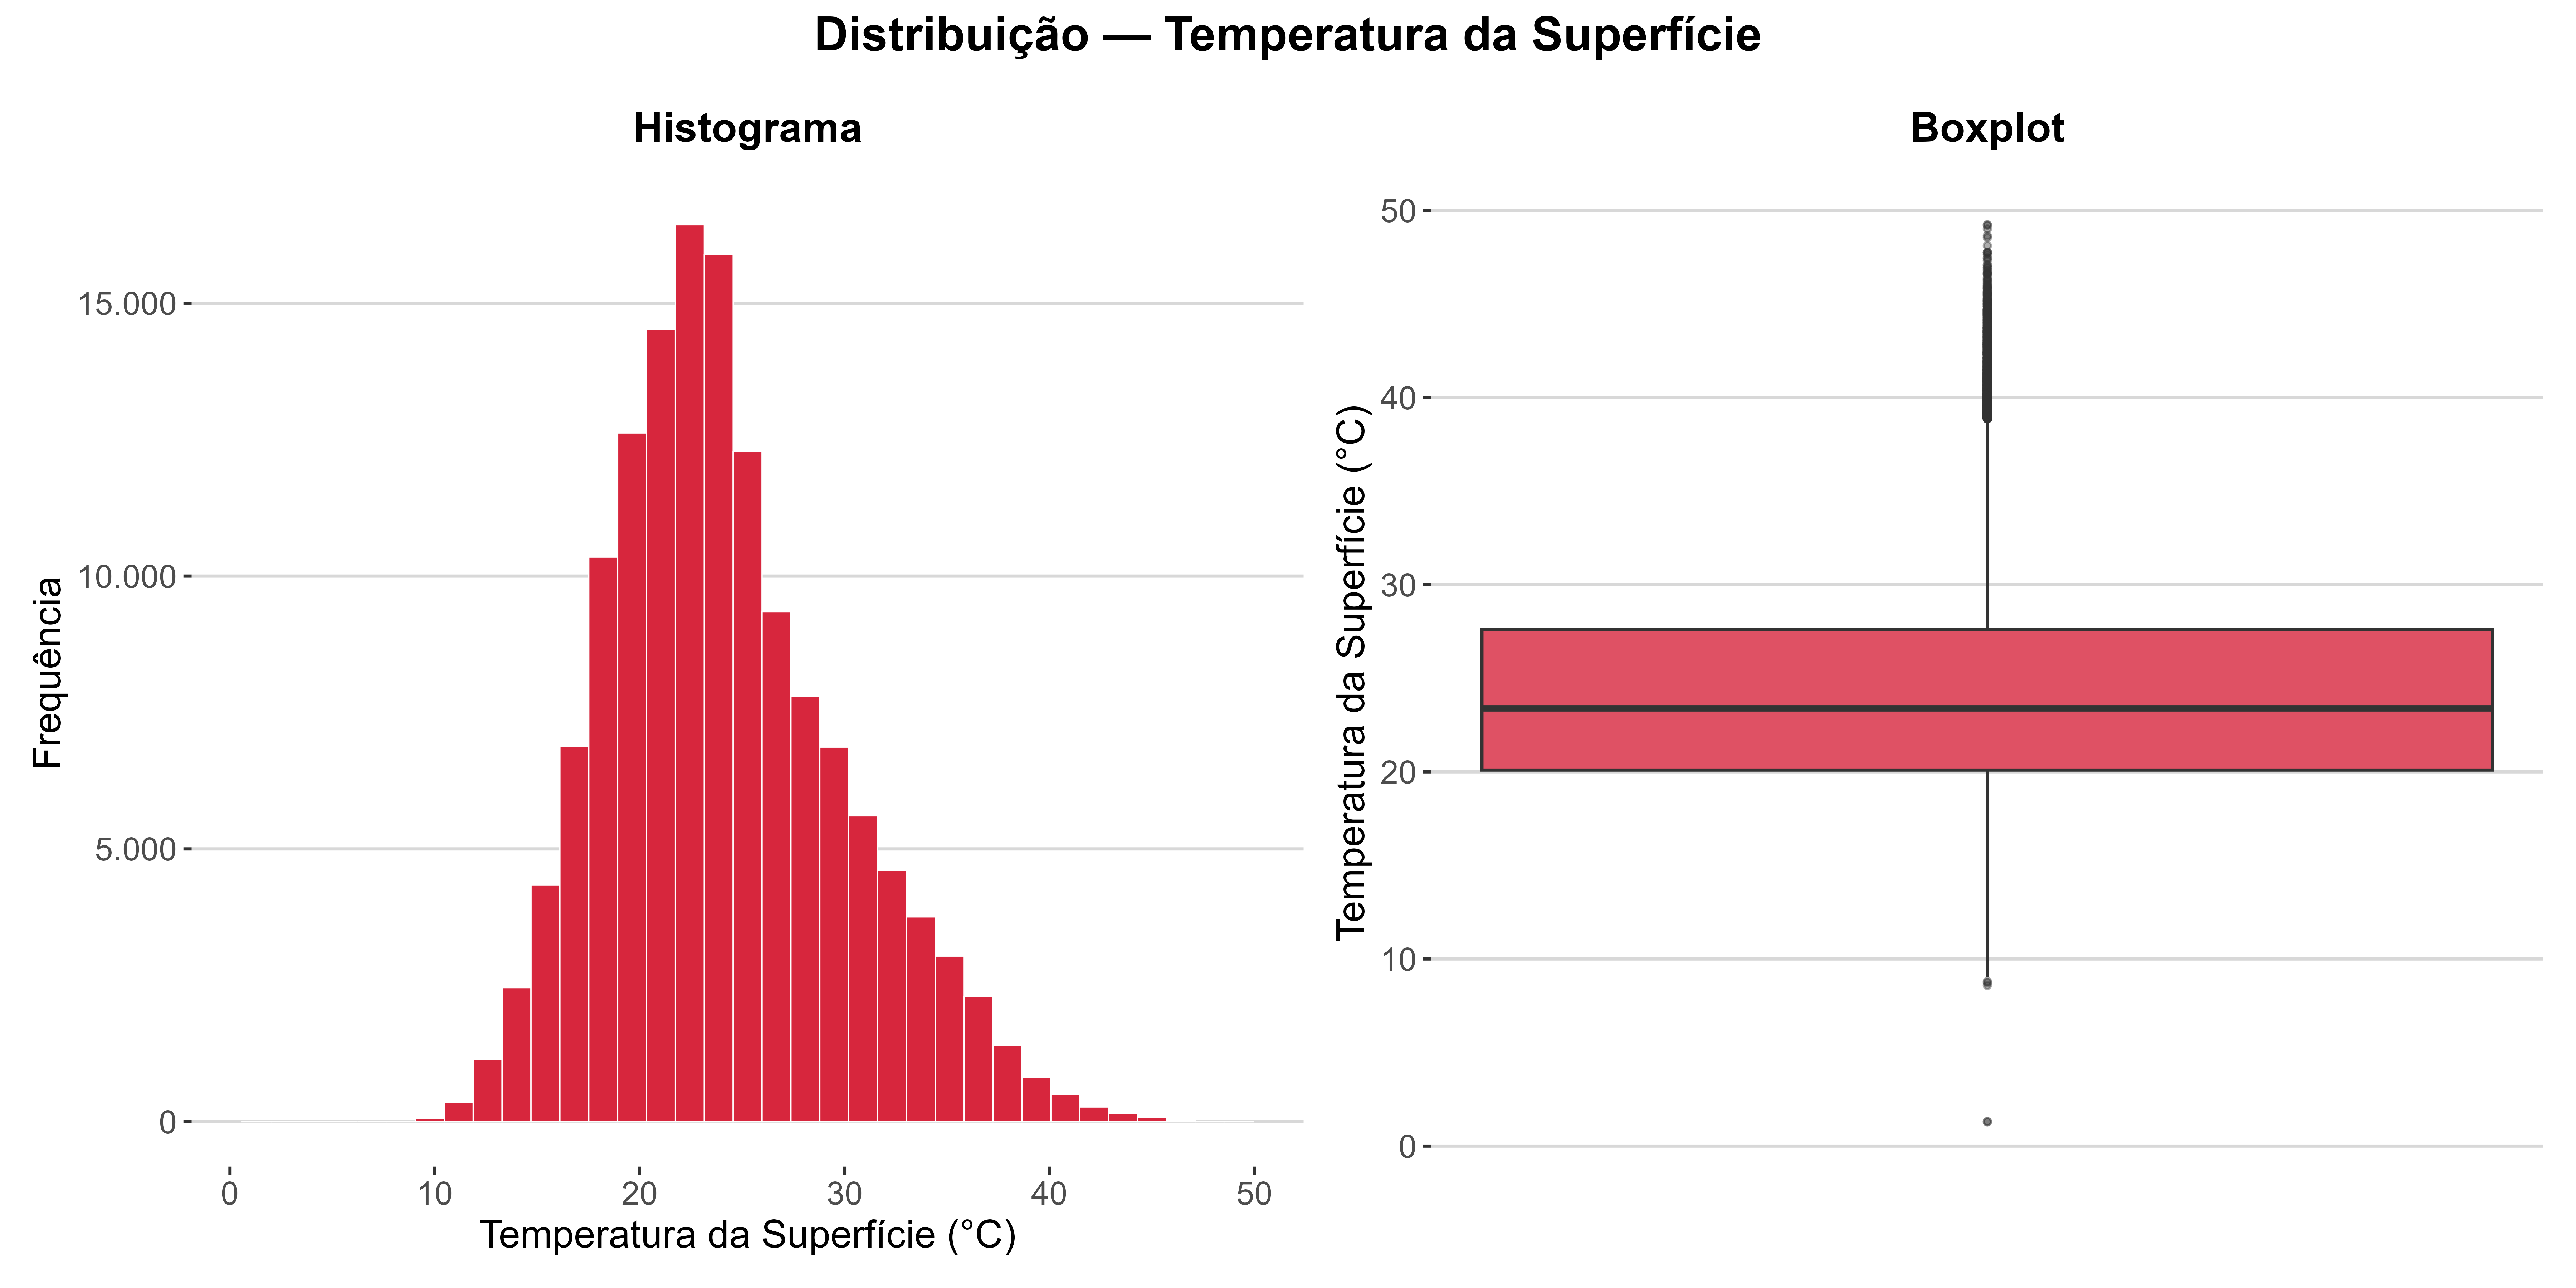
\includegraphics[keepaspectratio]{resultados/TempSuperficie/04_tempsuperficie_distribuicao.png}}

}

\caption{Distribuição da Temperatura da Superfície}

\end{figure}%

\paragraph{Principais Achados}\label{principais-achados-4}

A temperatura da superfície segue o mesmo padrão sazonal da temperatura
do ar, porém com \textbf{amplitudes consideravelmente maiores}: os picos
chegam a valores próximos de 50 °C nas séries horárias de verão,
enquanto os mínimos ficam em torno de 10--12 °C no inverno. Essa
diferença em relação à temperatura do ar reflete o aquecimento radiativo
direto da superfície terrestre.

A distribuição é \textbf{mais larga} do que a da temperatura do ar, com
maior dispersão nos valores altos. Isso sugere que a superfície é mais
sensível às variações de radiação solar, tornando essa variável um
preditor relevante para o modelo.

\subsubsection{Temperatura do Ponto de
Orvalho}\label{temperatura-do-ponto-de-orvalho}

\begin{figure}[H]

{\centering \pandocbounded{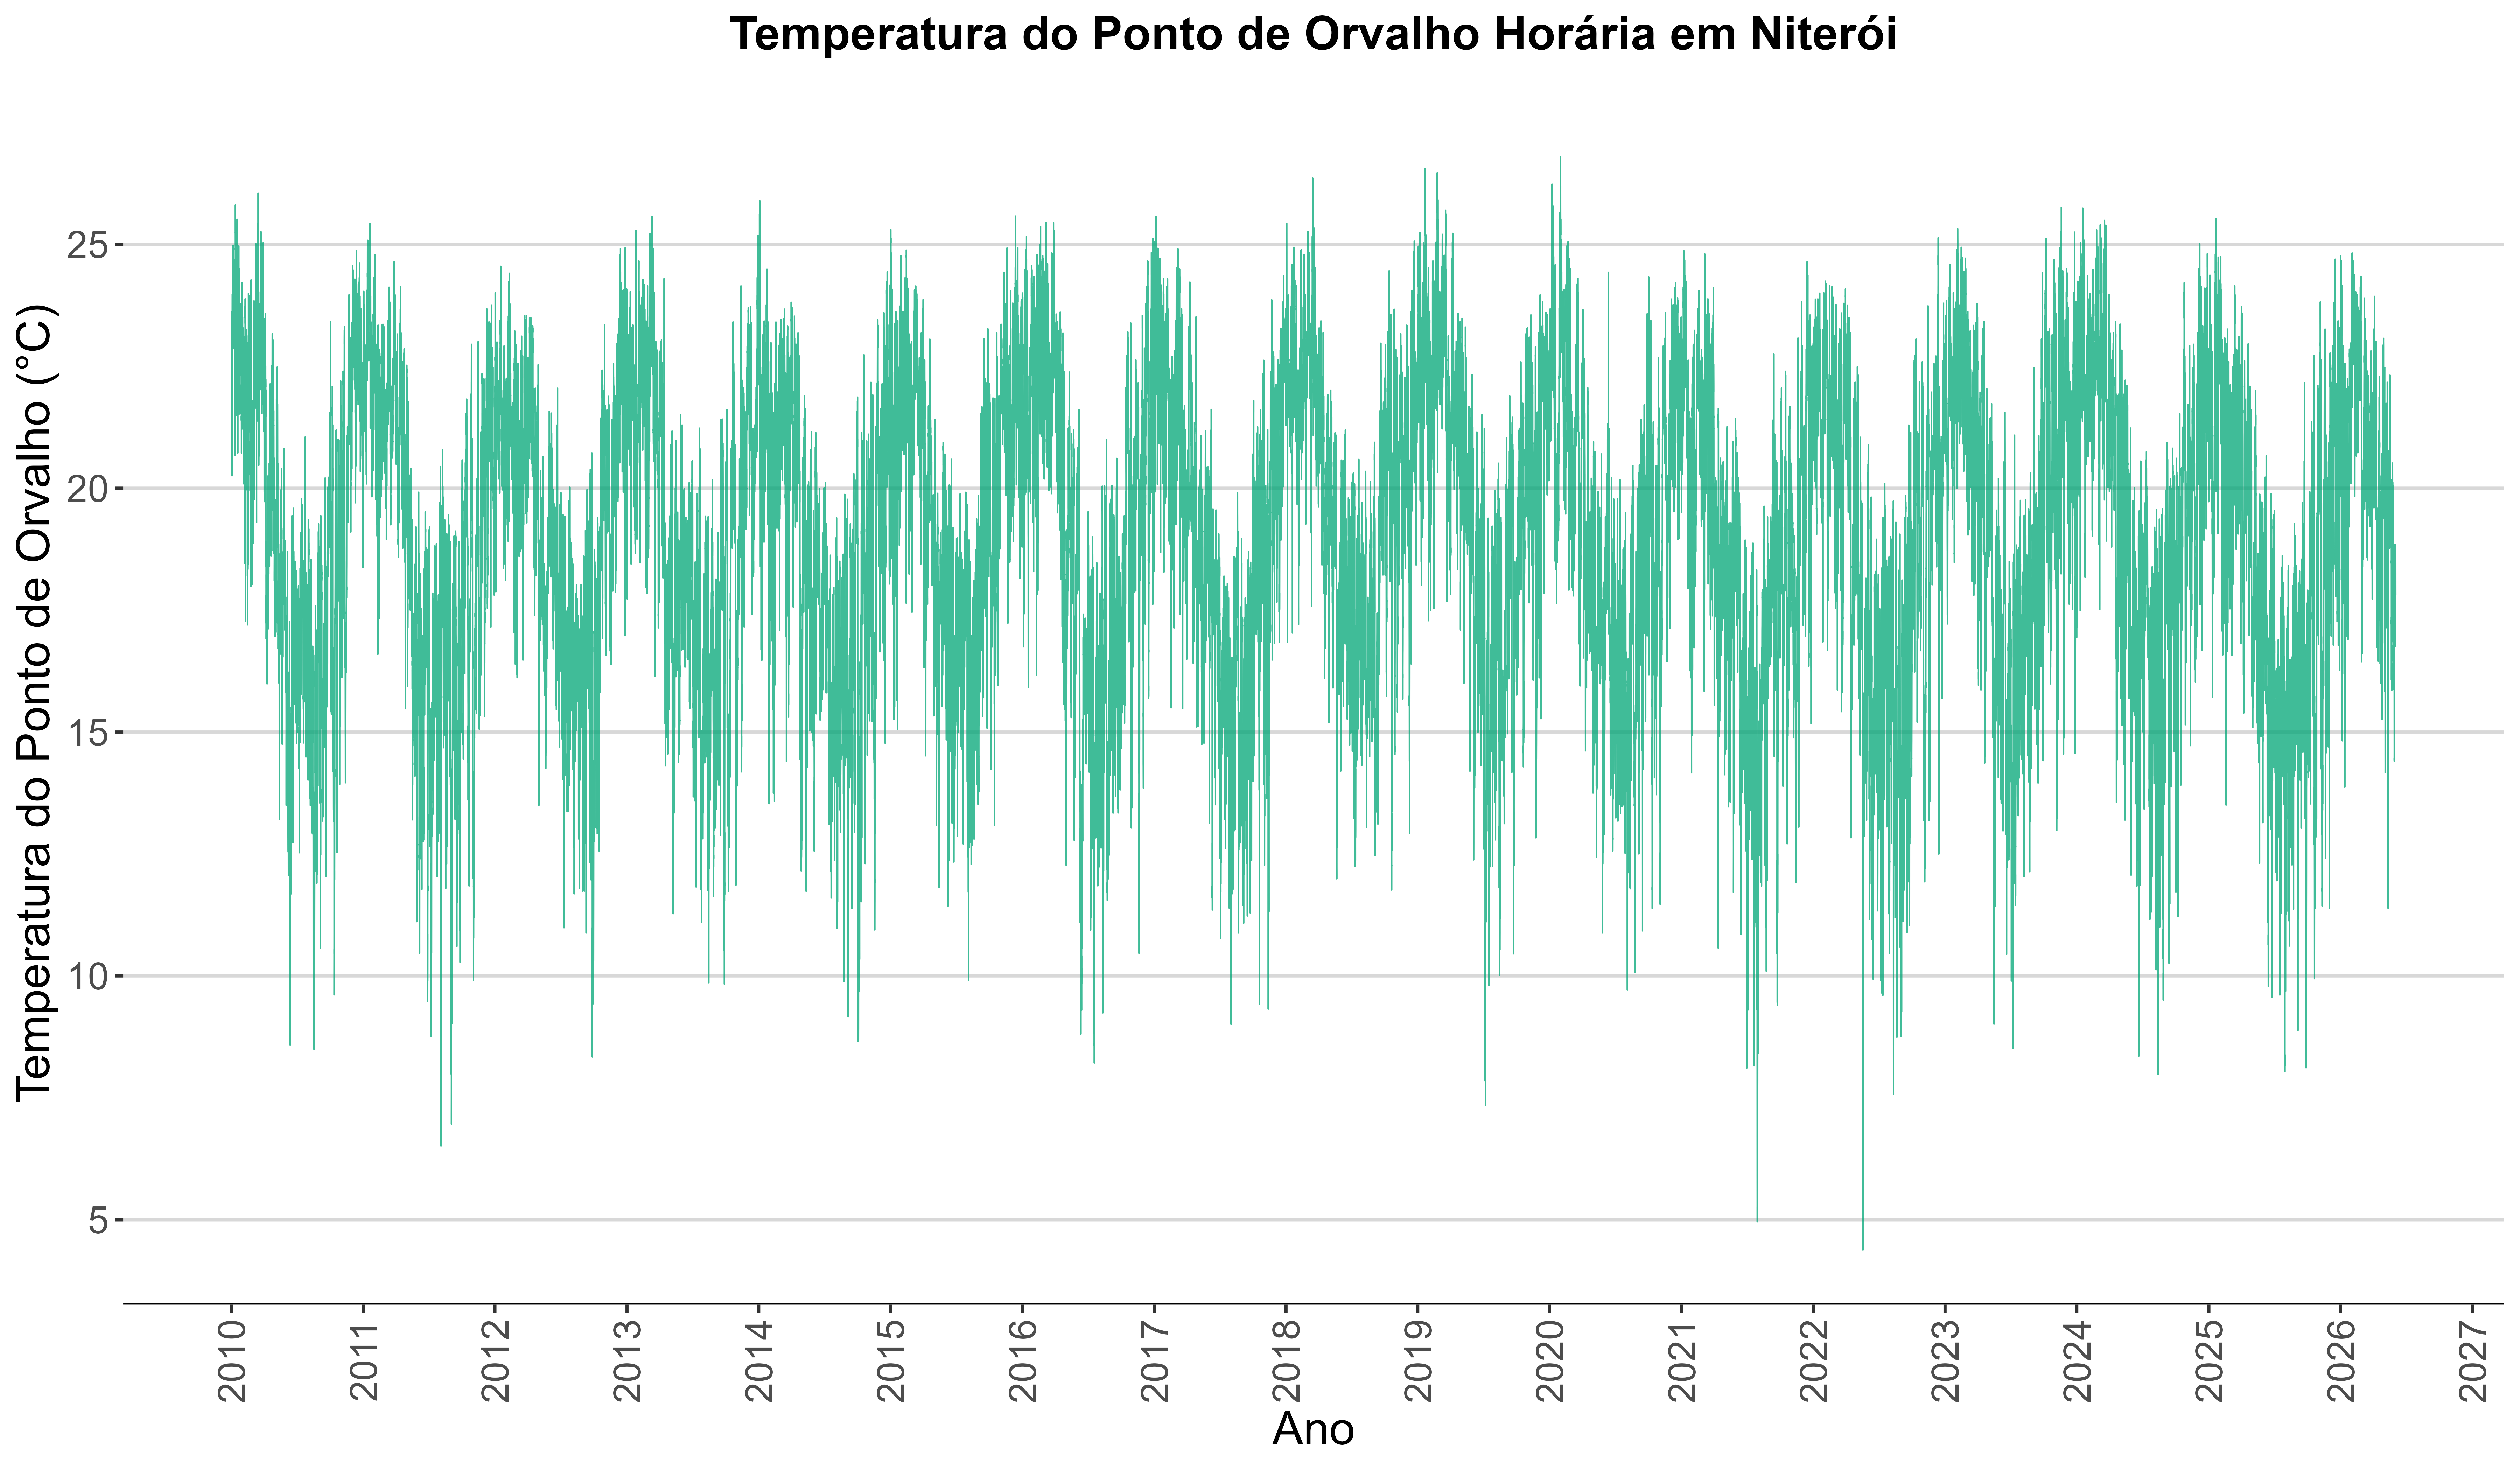
\includegraphics[keepaspectratio]{resultados/TempOrvalho/00_temporvalho_horario.png}}

}

\caption{Temperatura do Ponto de Orvalho Horária}

\end{figure}%

\begin{figure}[H]

{\centering \pandocbounded{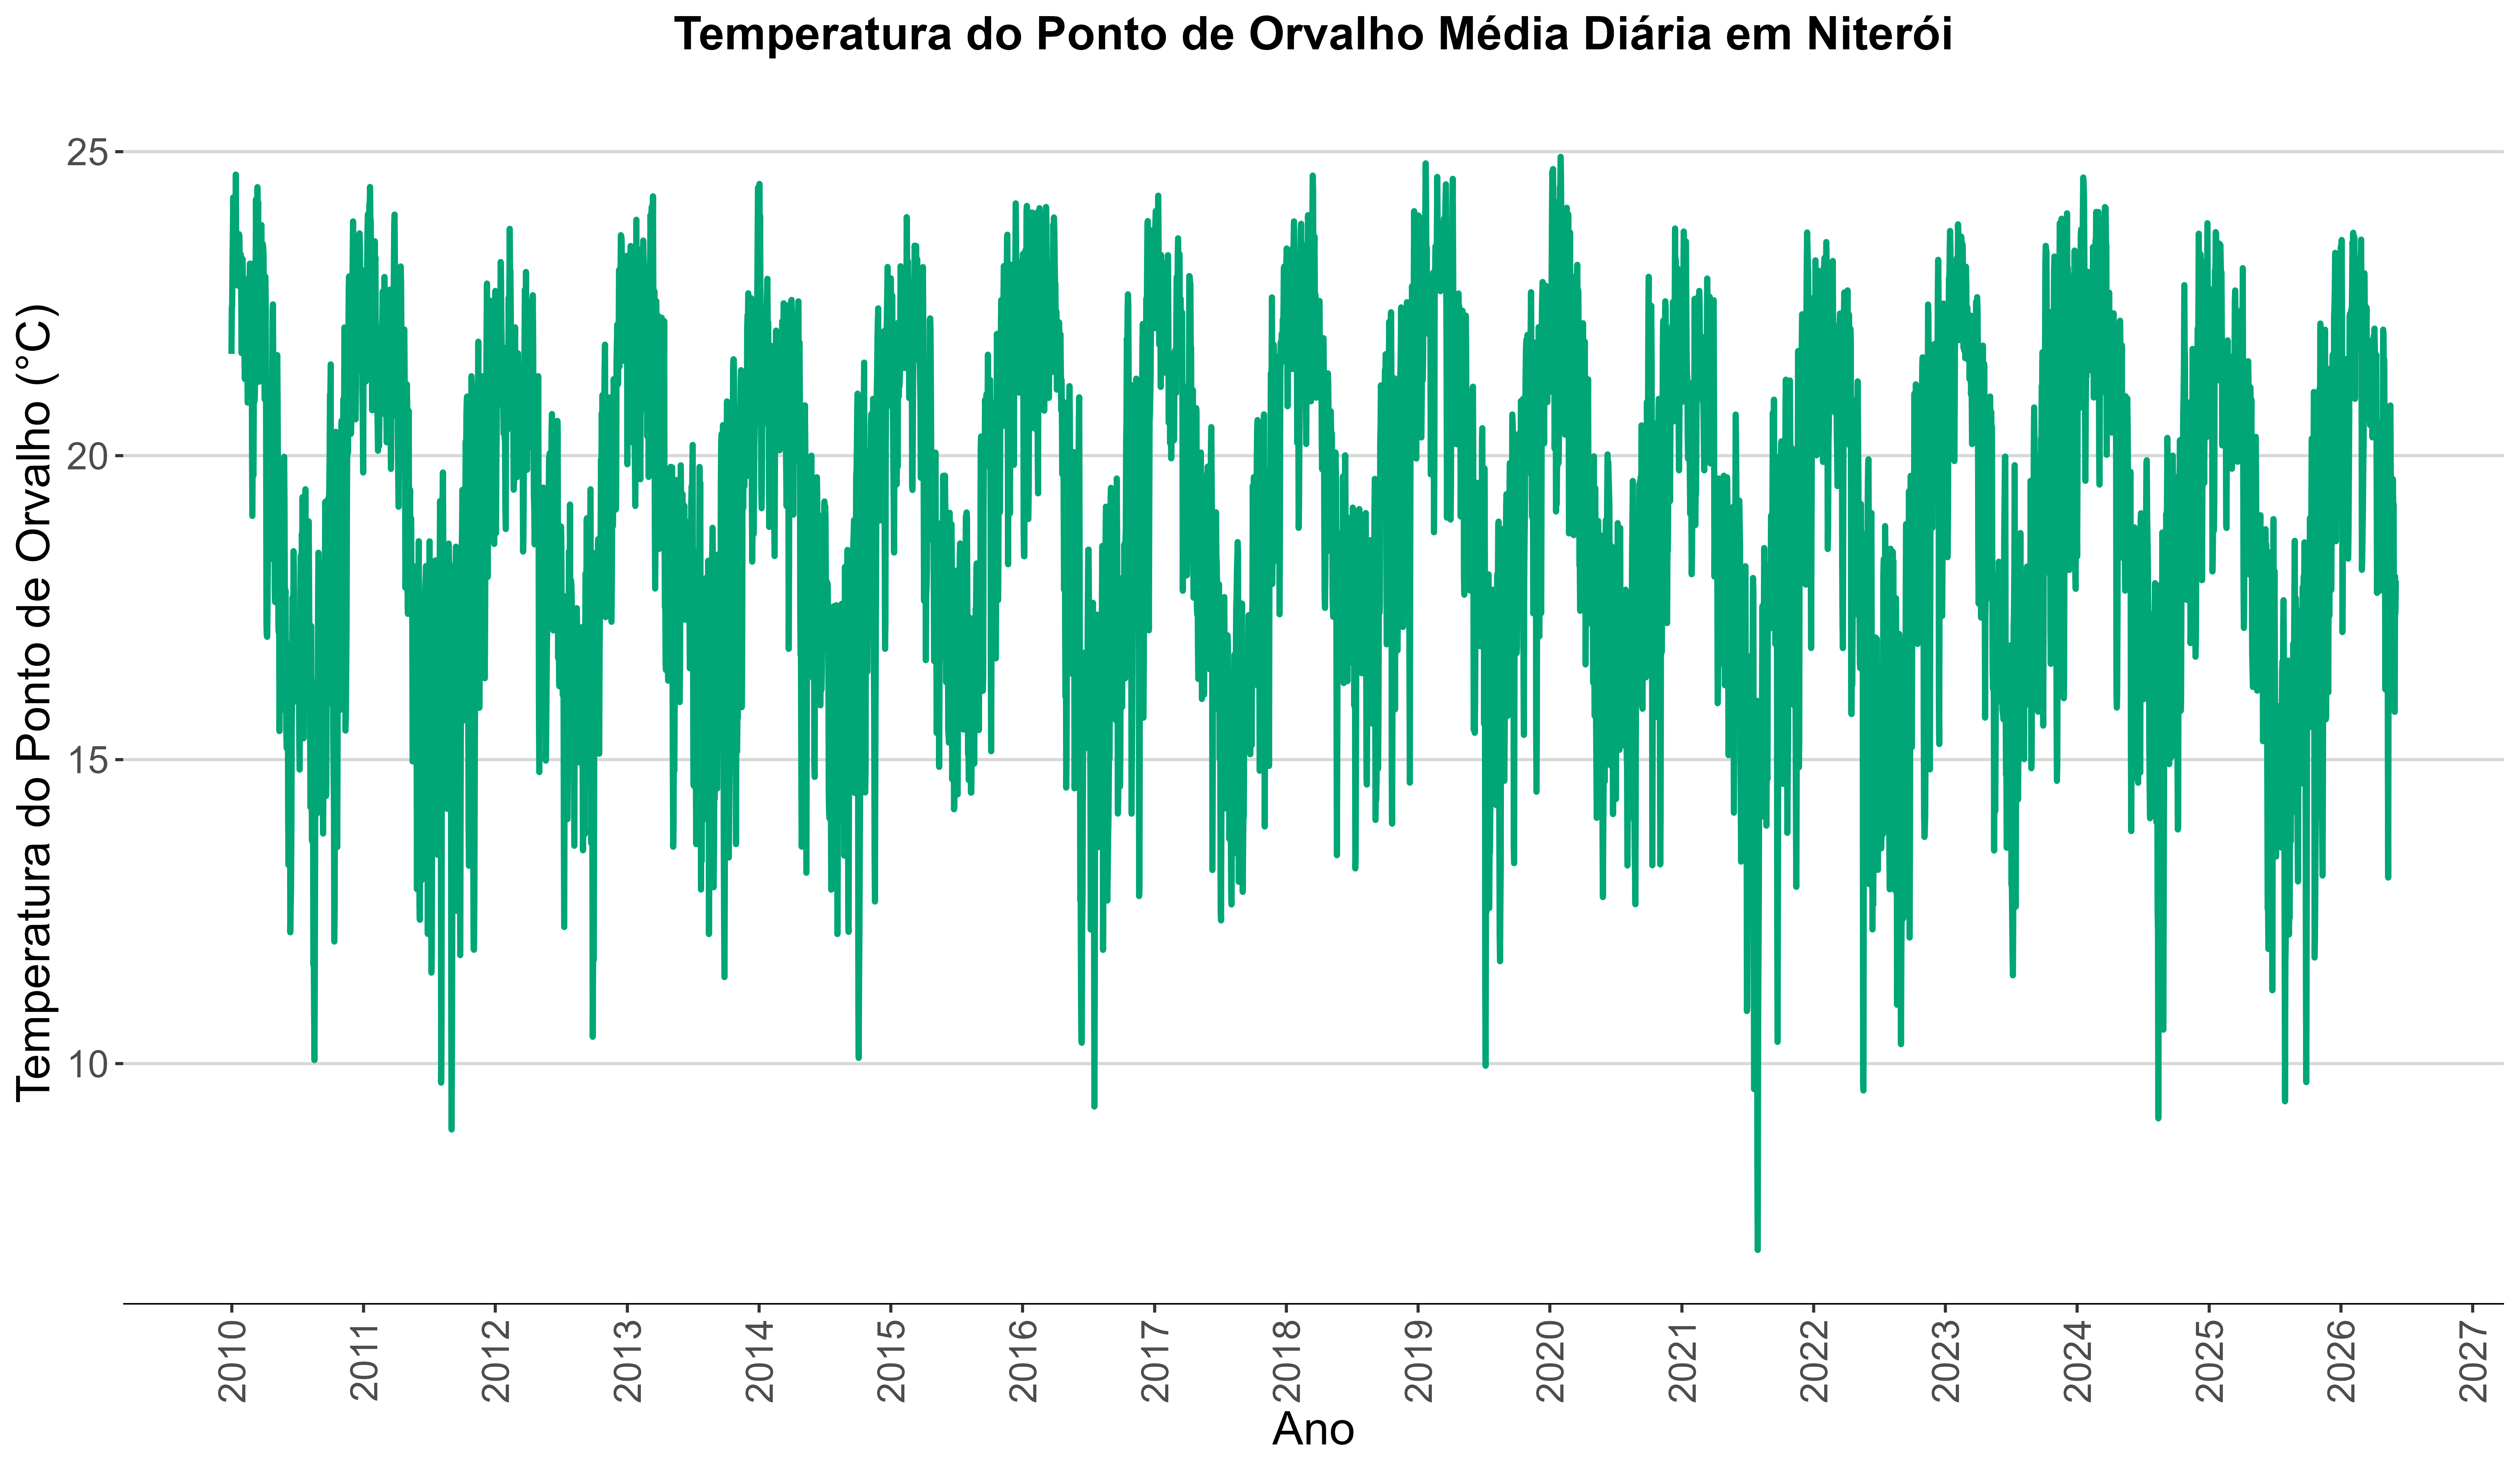
\includegraphics[keepaspectratio]{resultados/TempOrvalho/01_temporvalho_diario.png}}

}

\caption{Temperatura do Ponto de Orvalho Média Diária}

\end{figure}%

\begin{figure}[H]

{\centering \pandocbounded{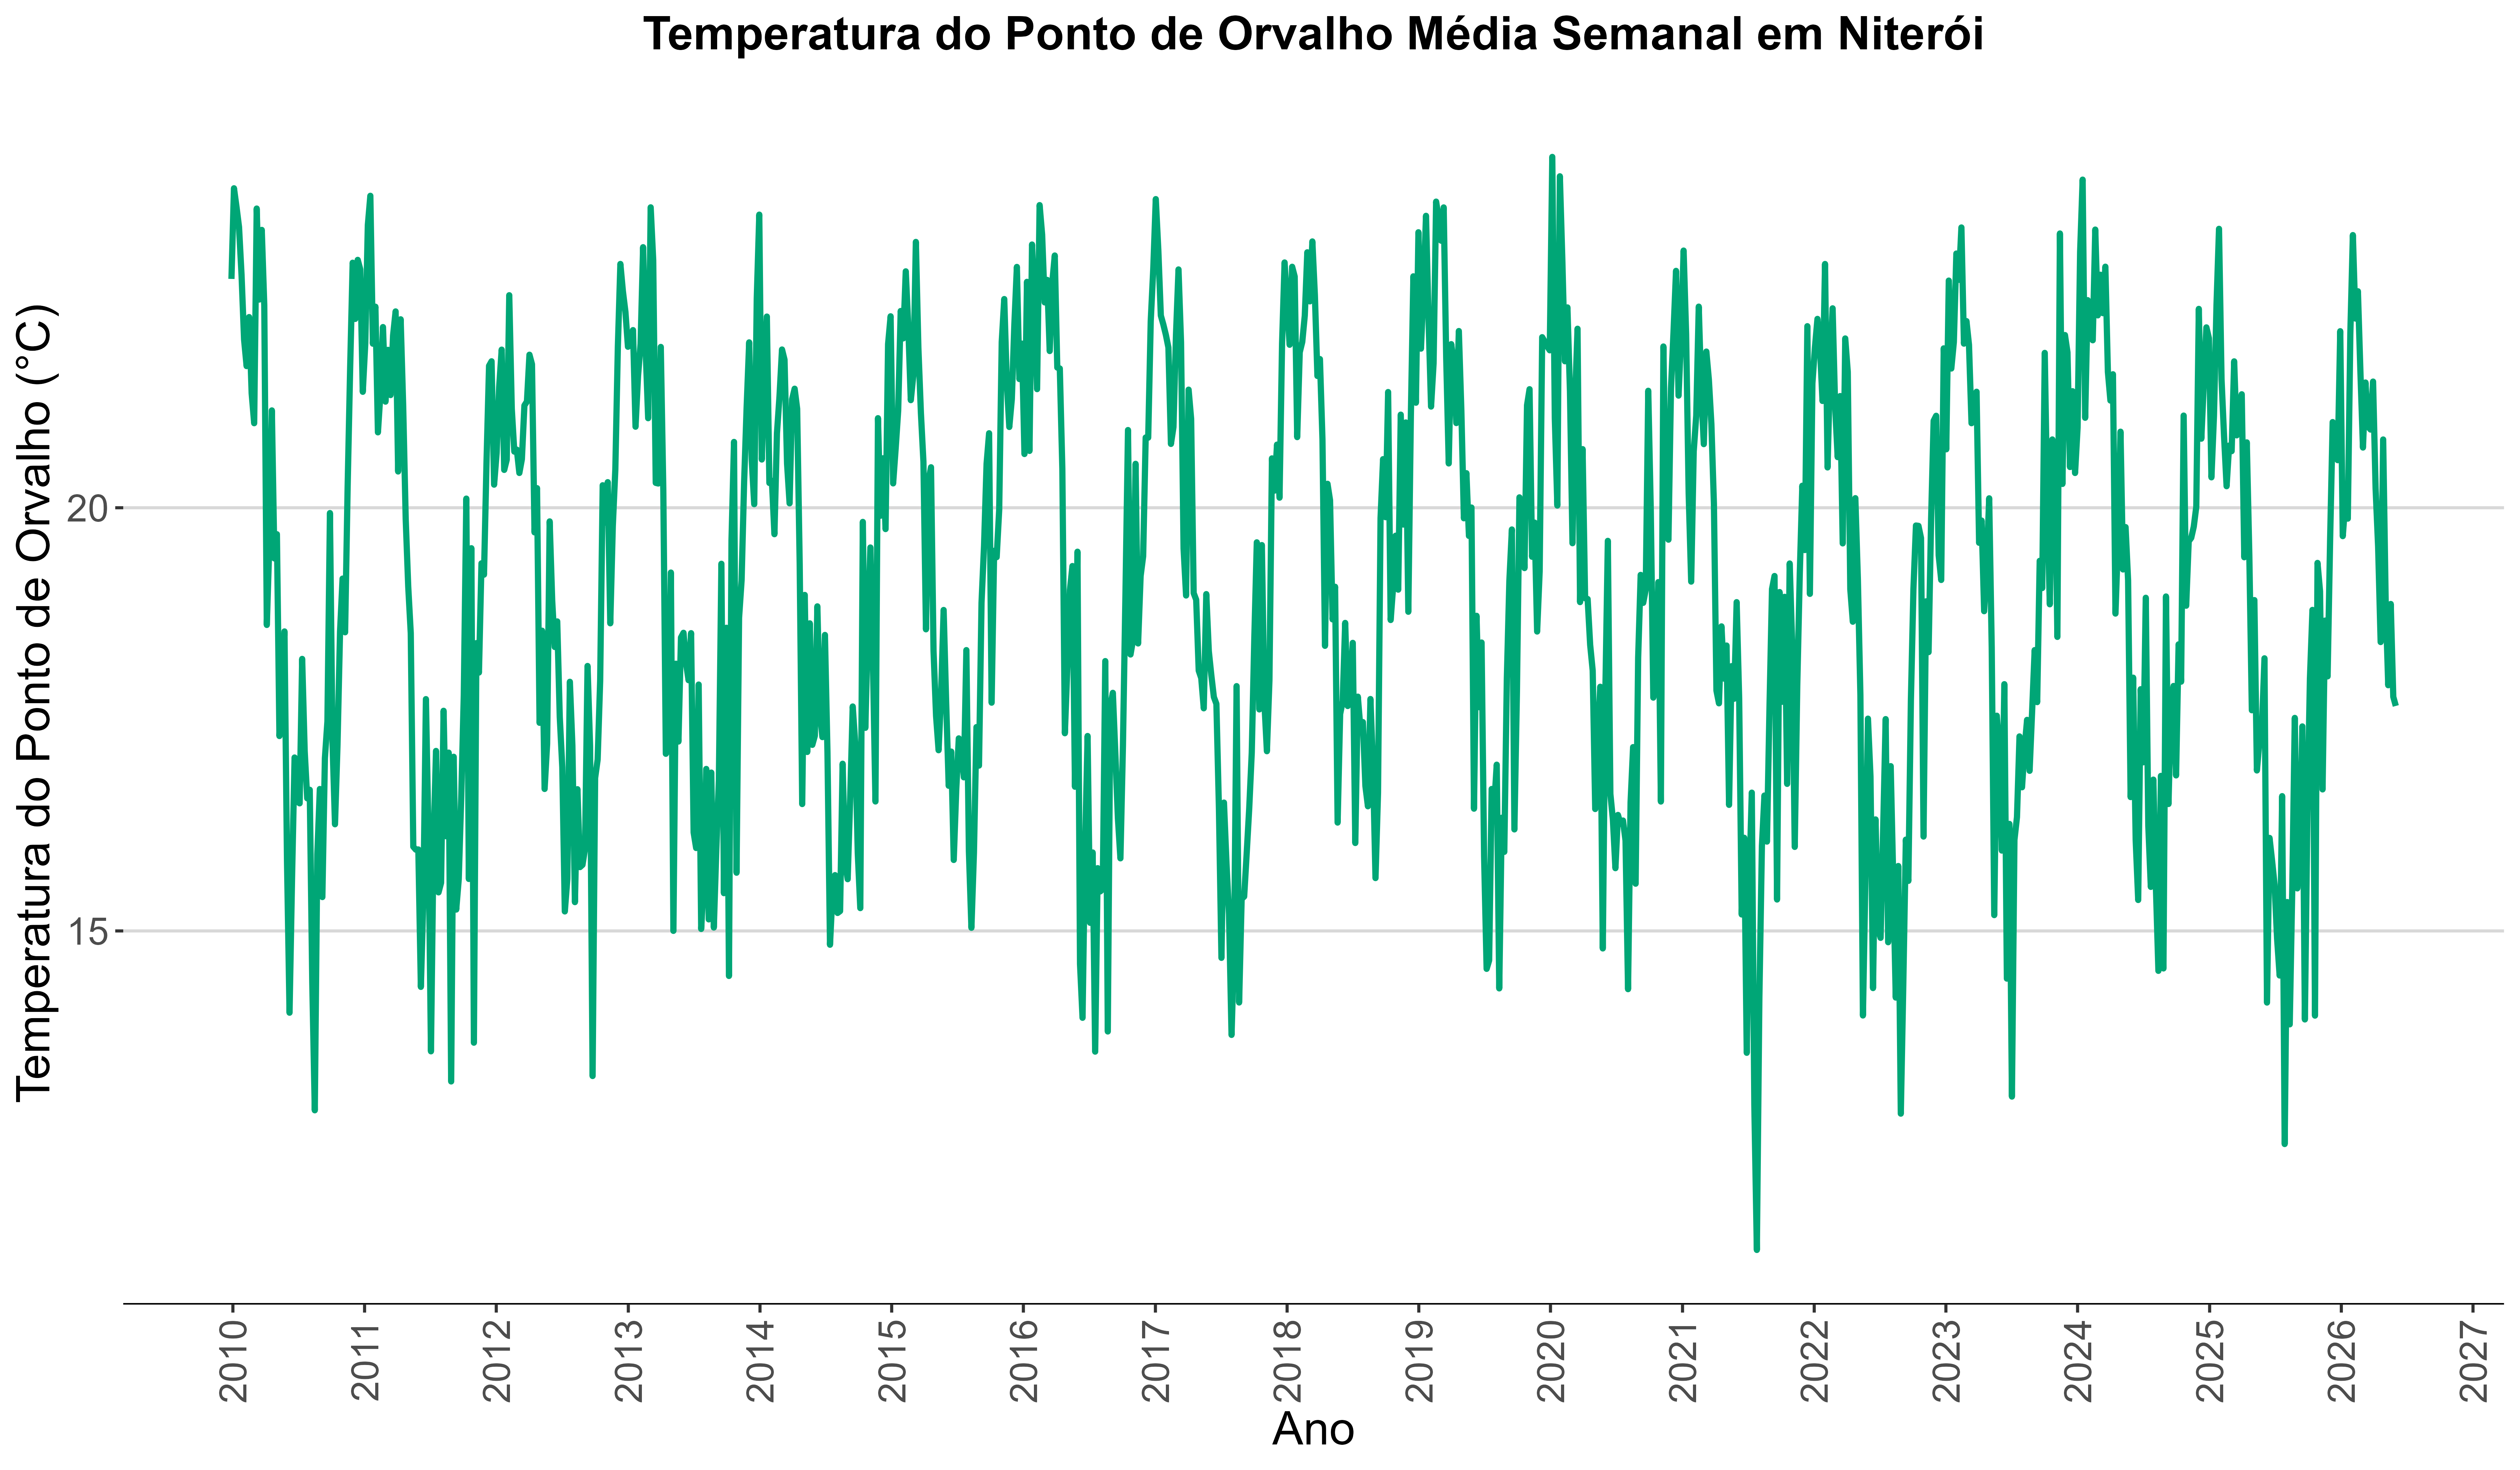
\includegraphics[keepaspectratio]{resultados/TempOrvalho/02_temporvalho_semanal.png}}

}

\caption{Temperatura do Ponto de Orvalho Média Semanal}

\end{figure}%

\begin{figure}[H]

{\centering \pandocbounded{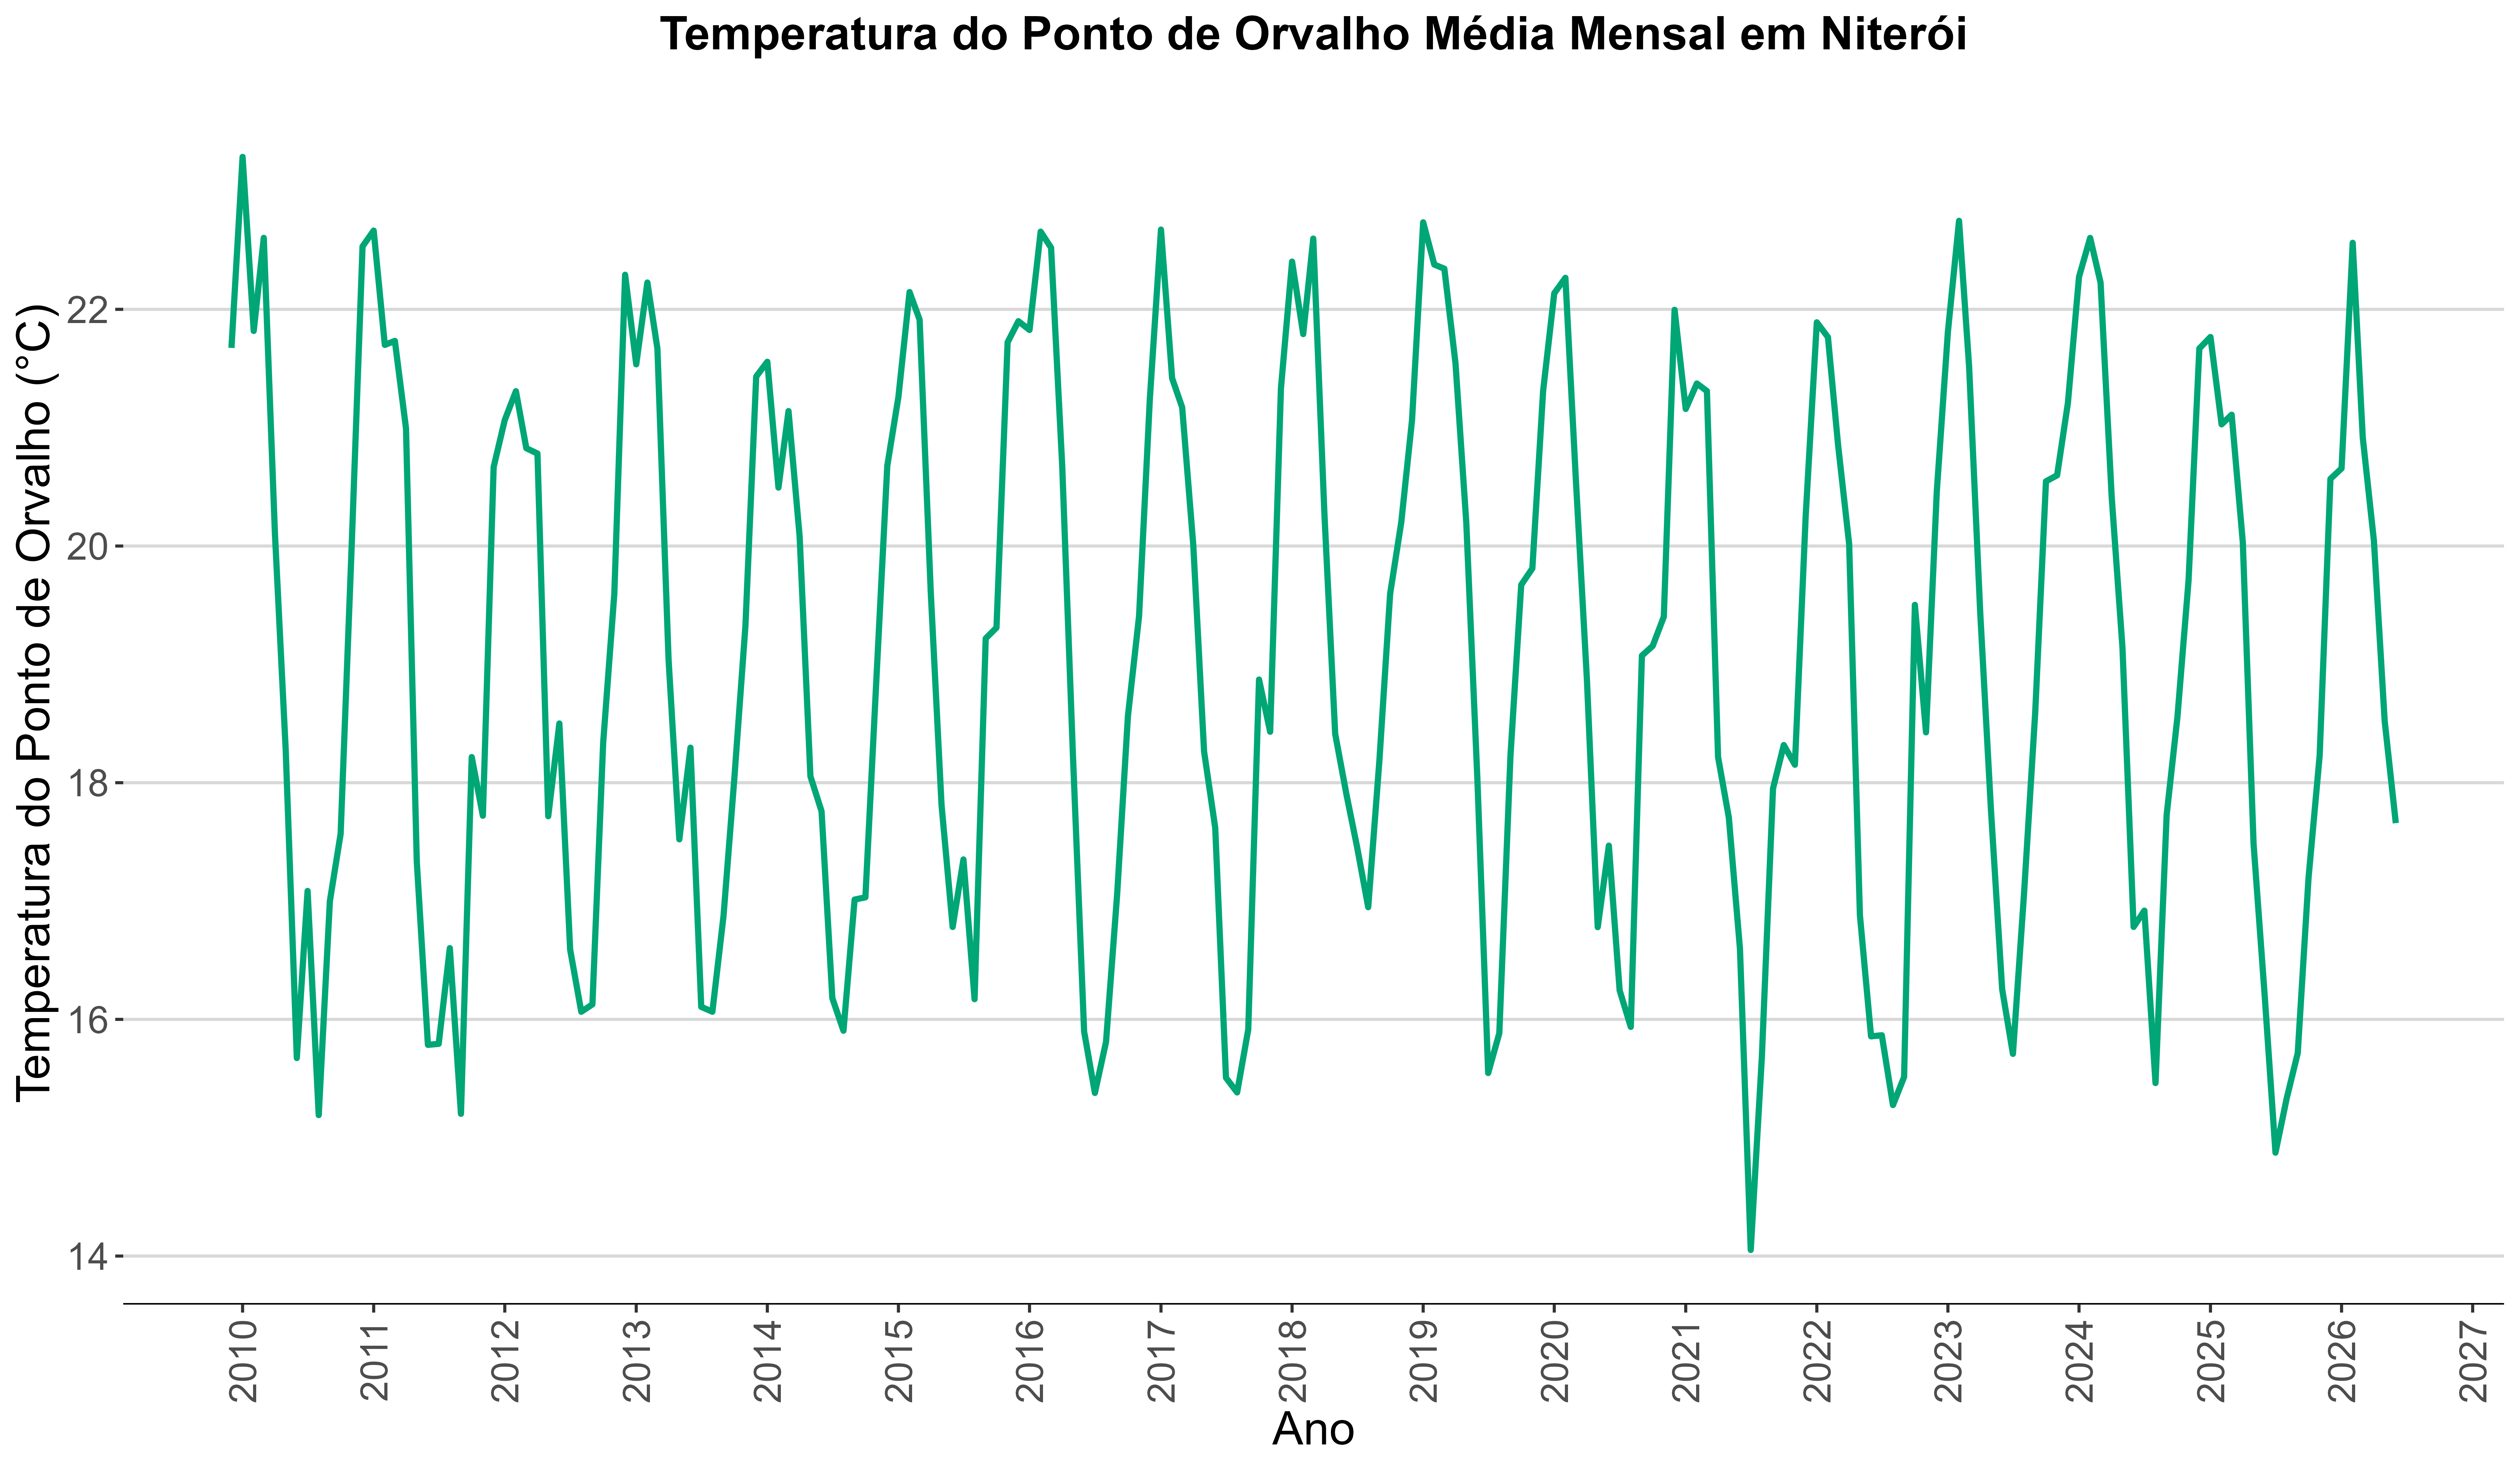
\includegraphics[keepaspectratio]{resultados/TempOrvalho/03_temporvalho_mensal.png}}

}

\caption{Temperatura do Ponto de Orvalho Média Mensal}

\end{figure}%

\begin{figure}[H]

{\centering \pandocbounded{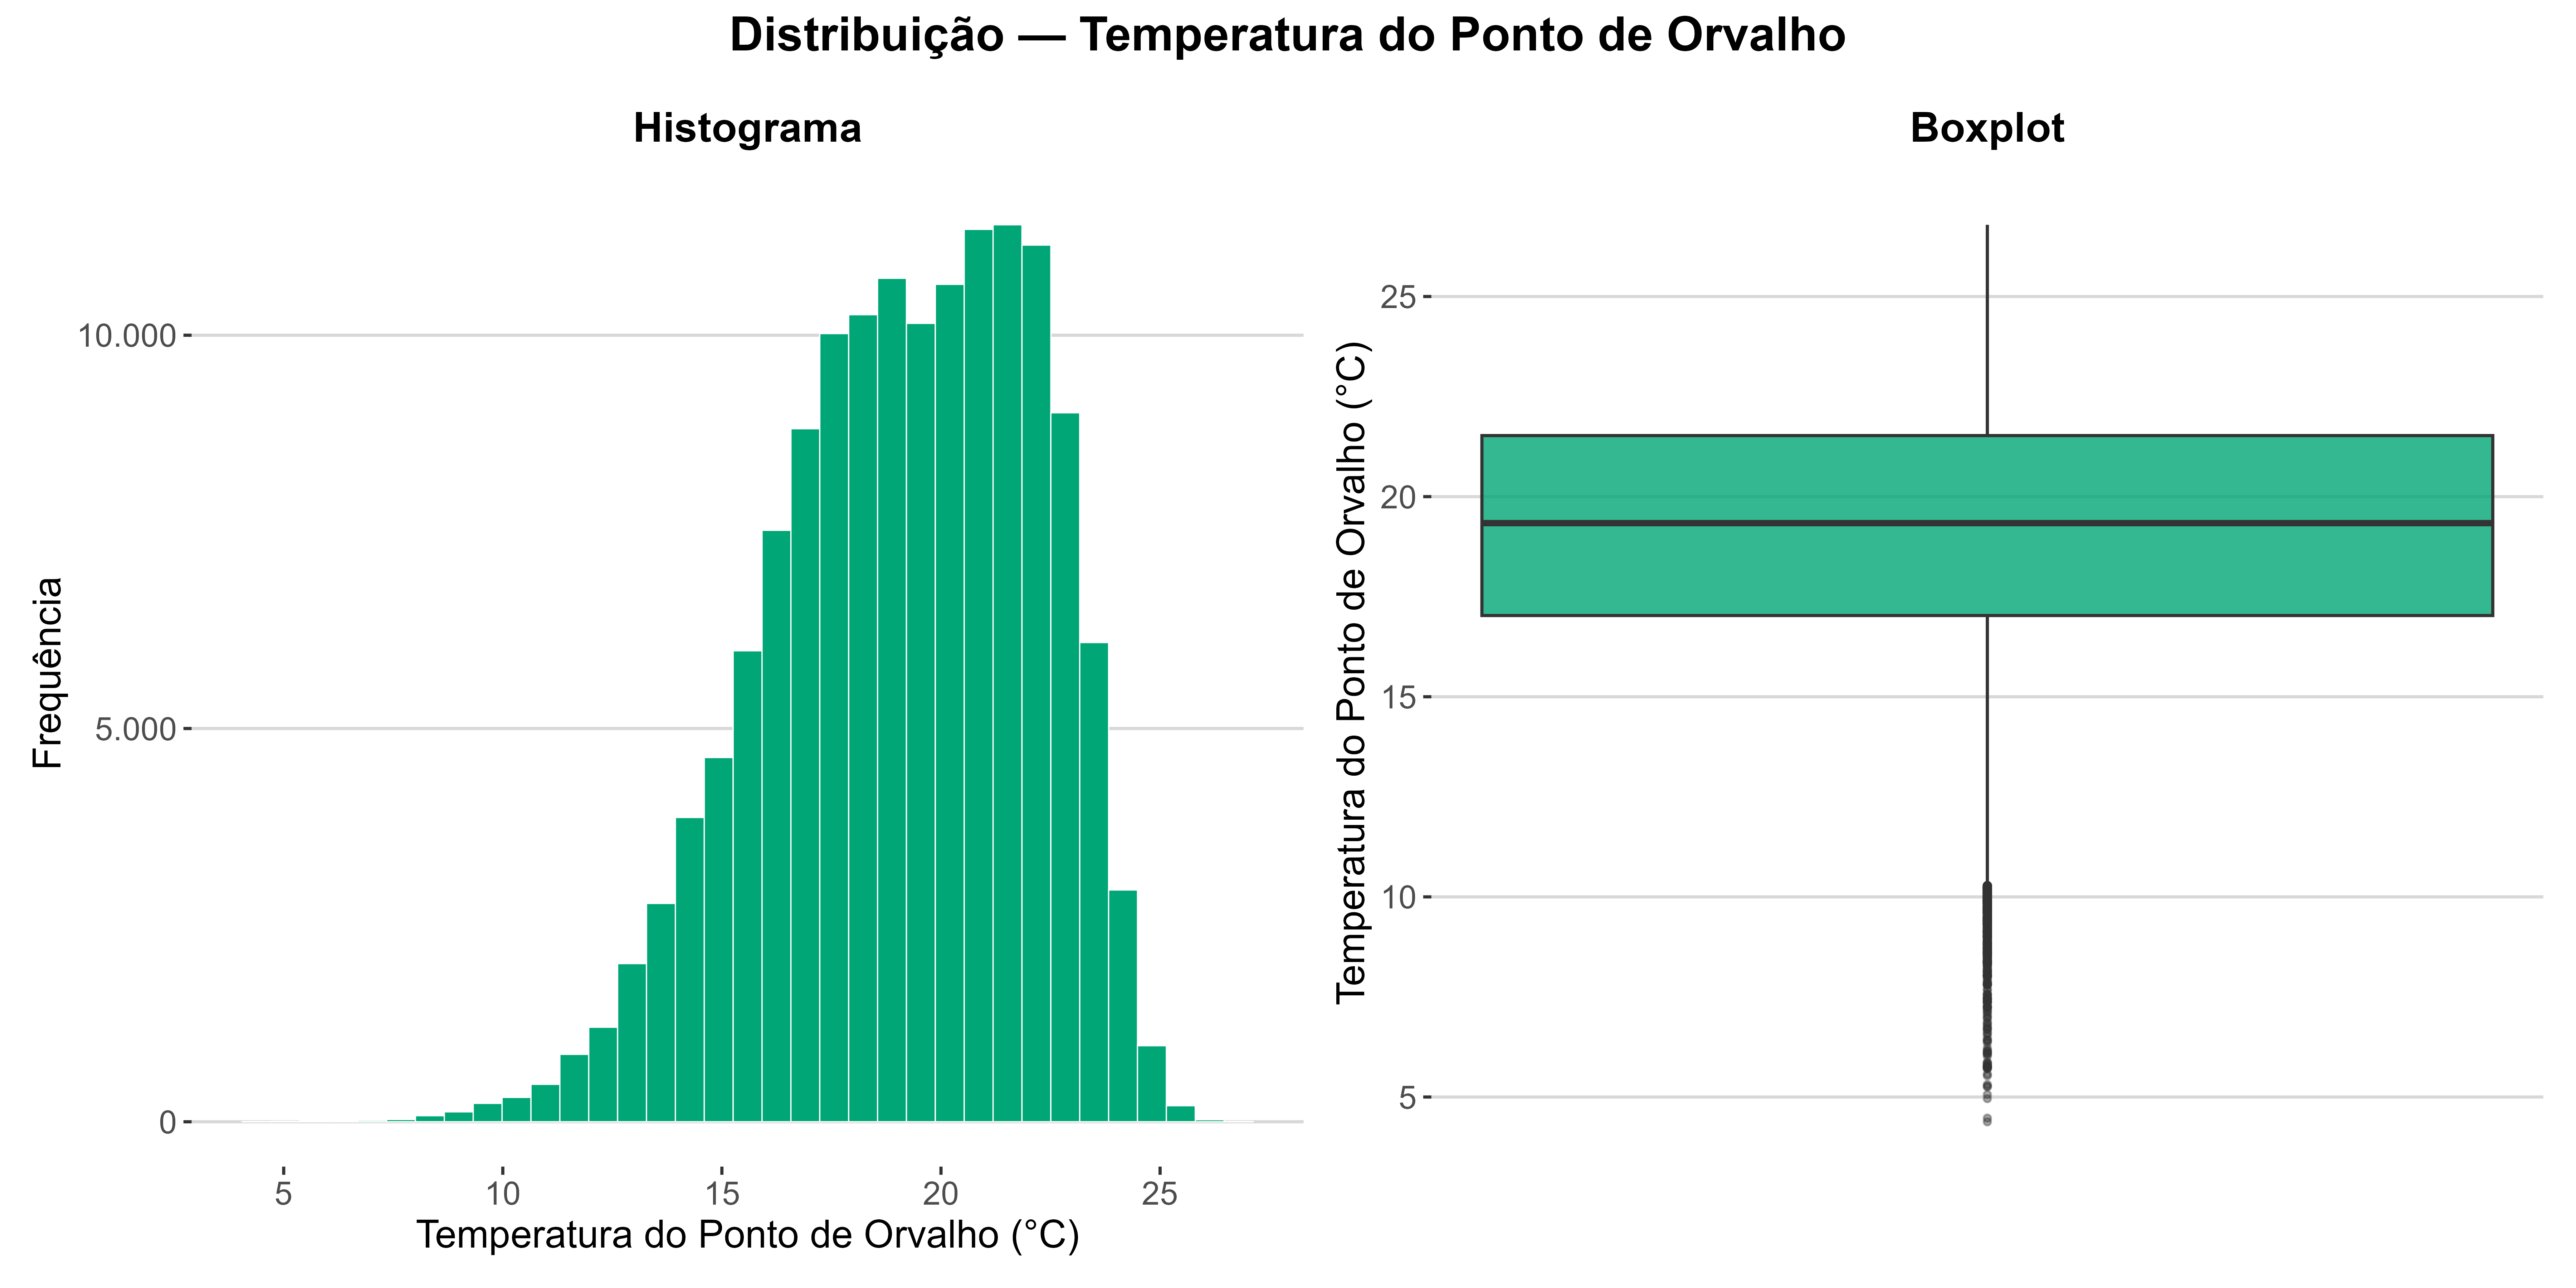
\includegraphics[keepaspectratio]{resultados/TempOrvalho/04_temporvalho_distribuicao.png}}

}

\caption{Distribuição da Temperatura do Ponto de Orvalho}

\end{figure}%

\paragraph{Principais Achados}\label{principais-achados-5}

A temperatura do ponto de orvalho acompanha a temperatura do ar,
mantendo-se geralmente entre 15 °C e 25 °C ao longo do ano, com
sazonalidade anual clara. Os valores mais baixos (abaixo de 10 °C)
ocorrem raramente e concentram-se nos invernos mais secos.

A distribuição é \textbf{mais asimétrica e estreita} do que a da
temperatura do ar, refletindo a maior estabilidade da umidade absoluta
em regiões litorâneas. A proximidade entre a temperatura do ar e a do
ponto de orvalho na maior parte do tempo confirma a alta umidade
relativa característica de Niterói.

\subsubsection{Radiação Solar
Líquida}\label{radiauxe7uxe3o-solar-luxedquida}

\begin{figure}[H]

{\centering \pandocbounded{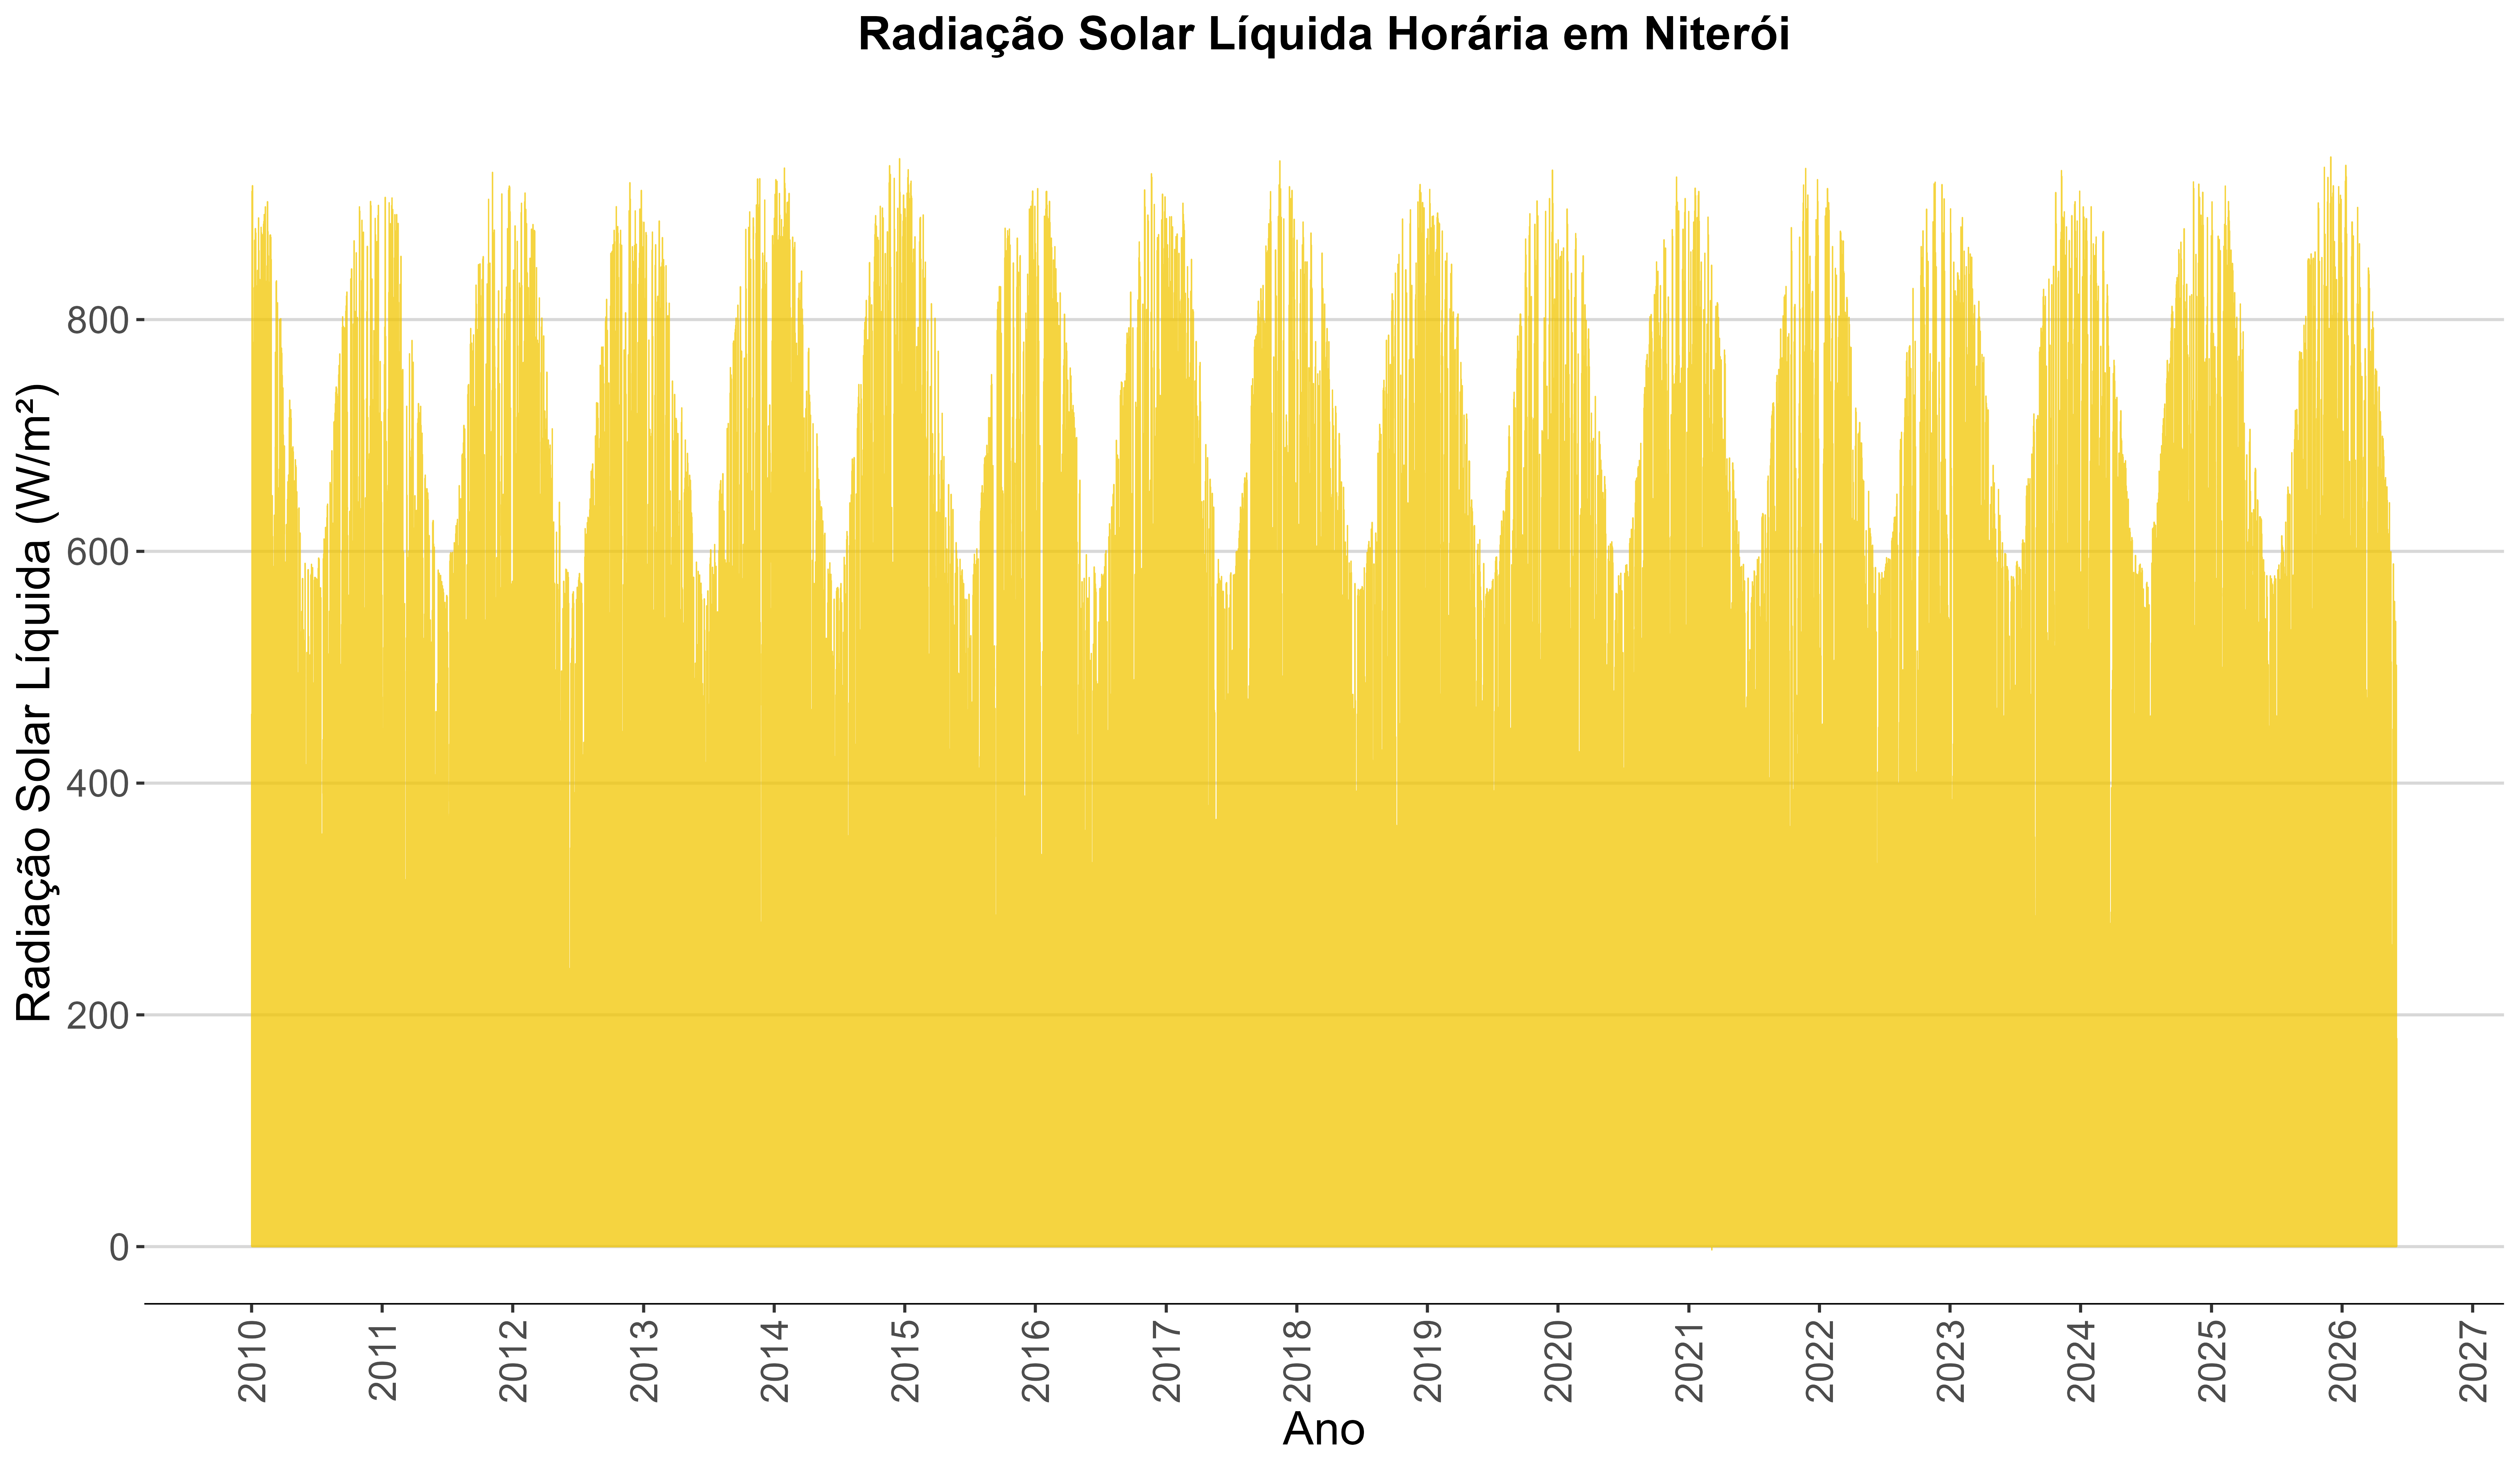
\includegraphics[keepaspectratio]{resultados/RadiacaoSolar/00_radiacaosolar_horario.png}}

}

\caption{Radiação Solar Líquida Horária}

\end{figure}%

\begin{figure}[H]

{\centering \pandocbounded{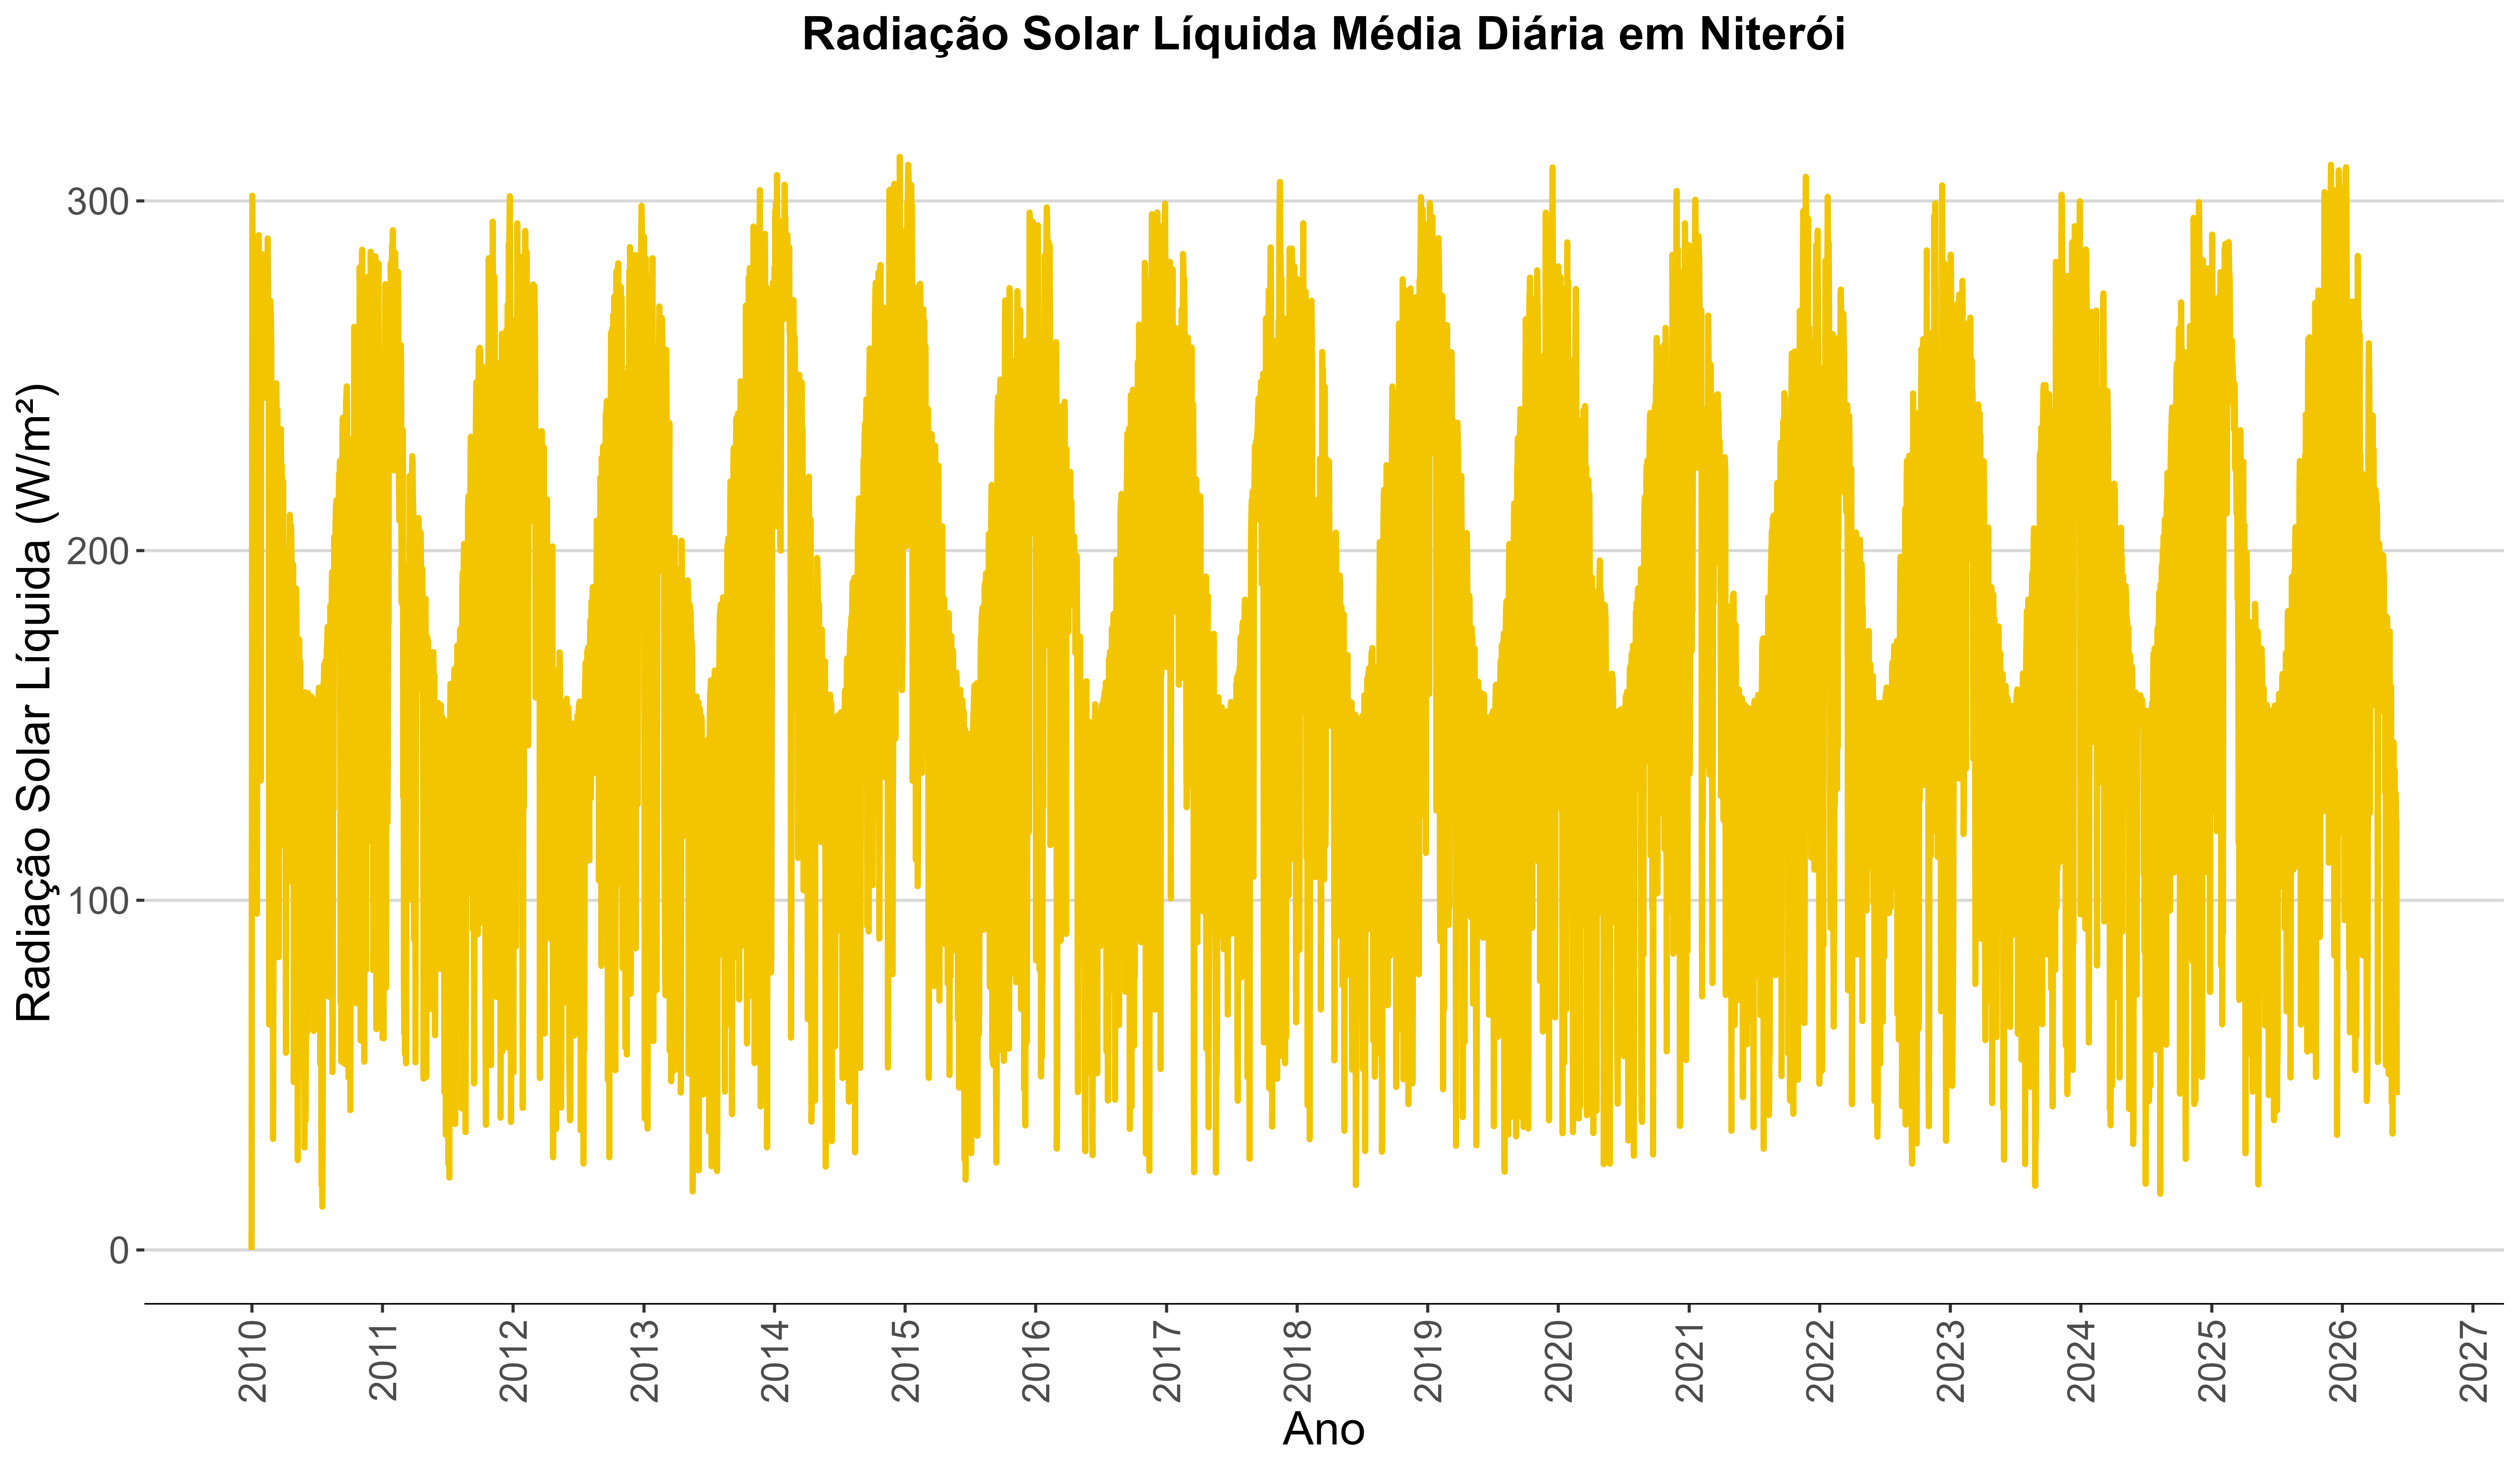
\includegraphics[keepaspectratio]{resultados/RadiacaoSolar/01_radiacaosolar_diario.png}}

}

\caption{Radiação Solar Líquida Média Diária}

\end{figure}%

\begin{figure}[H]

{\centering \pandocbounded{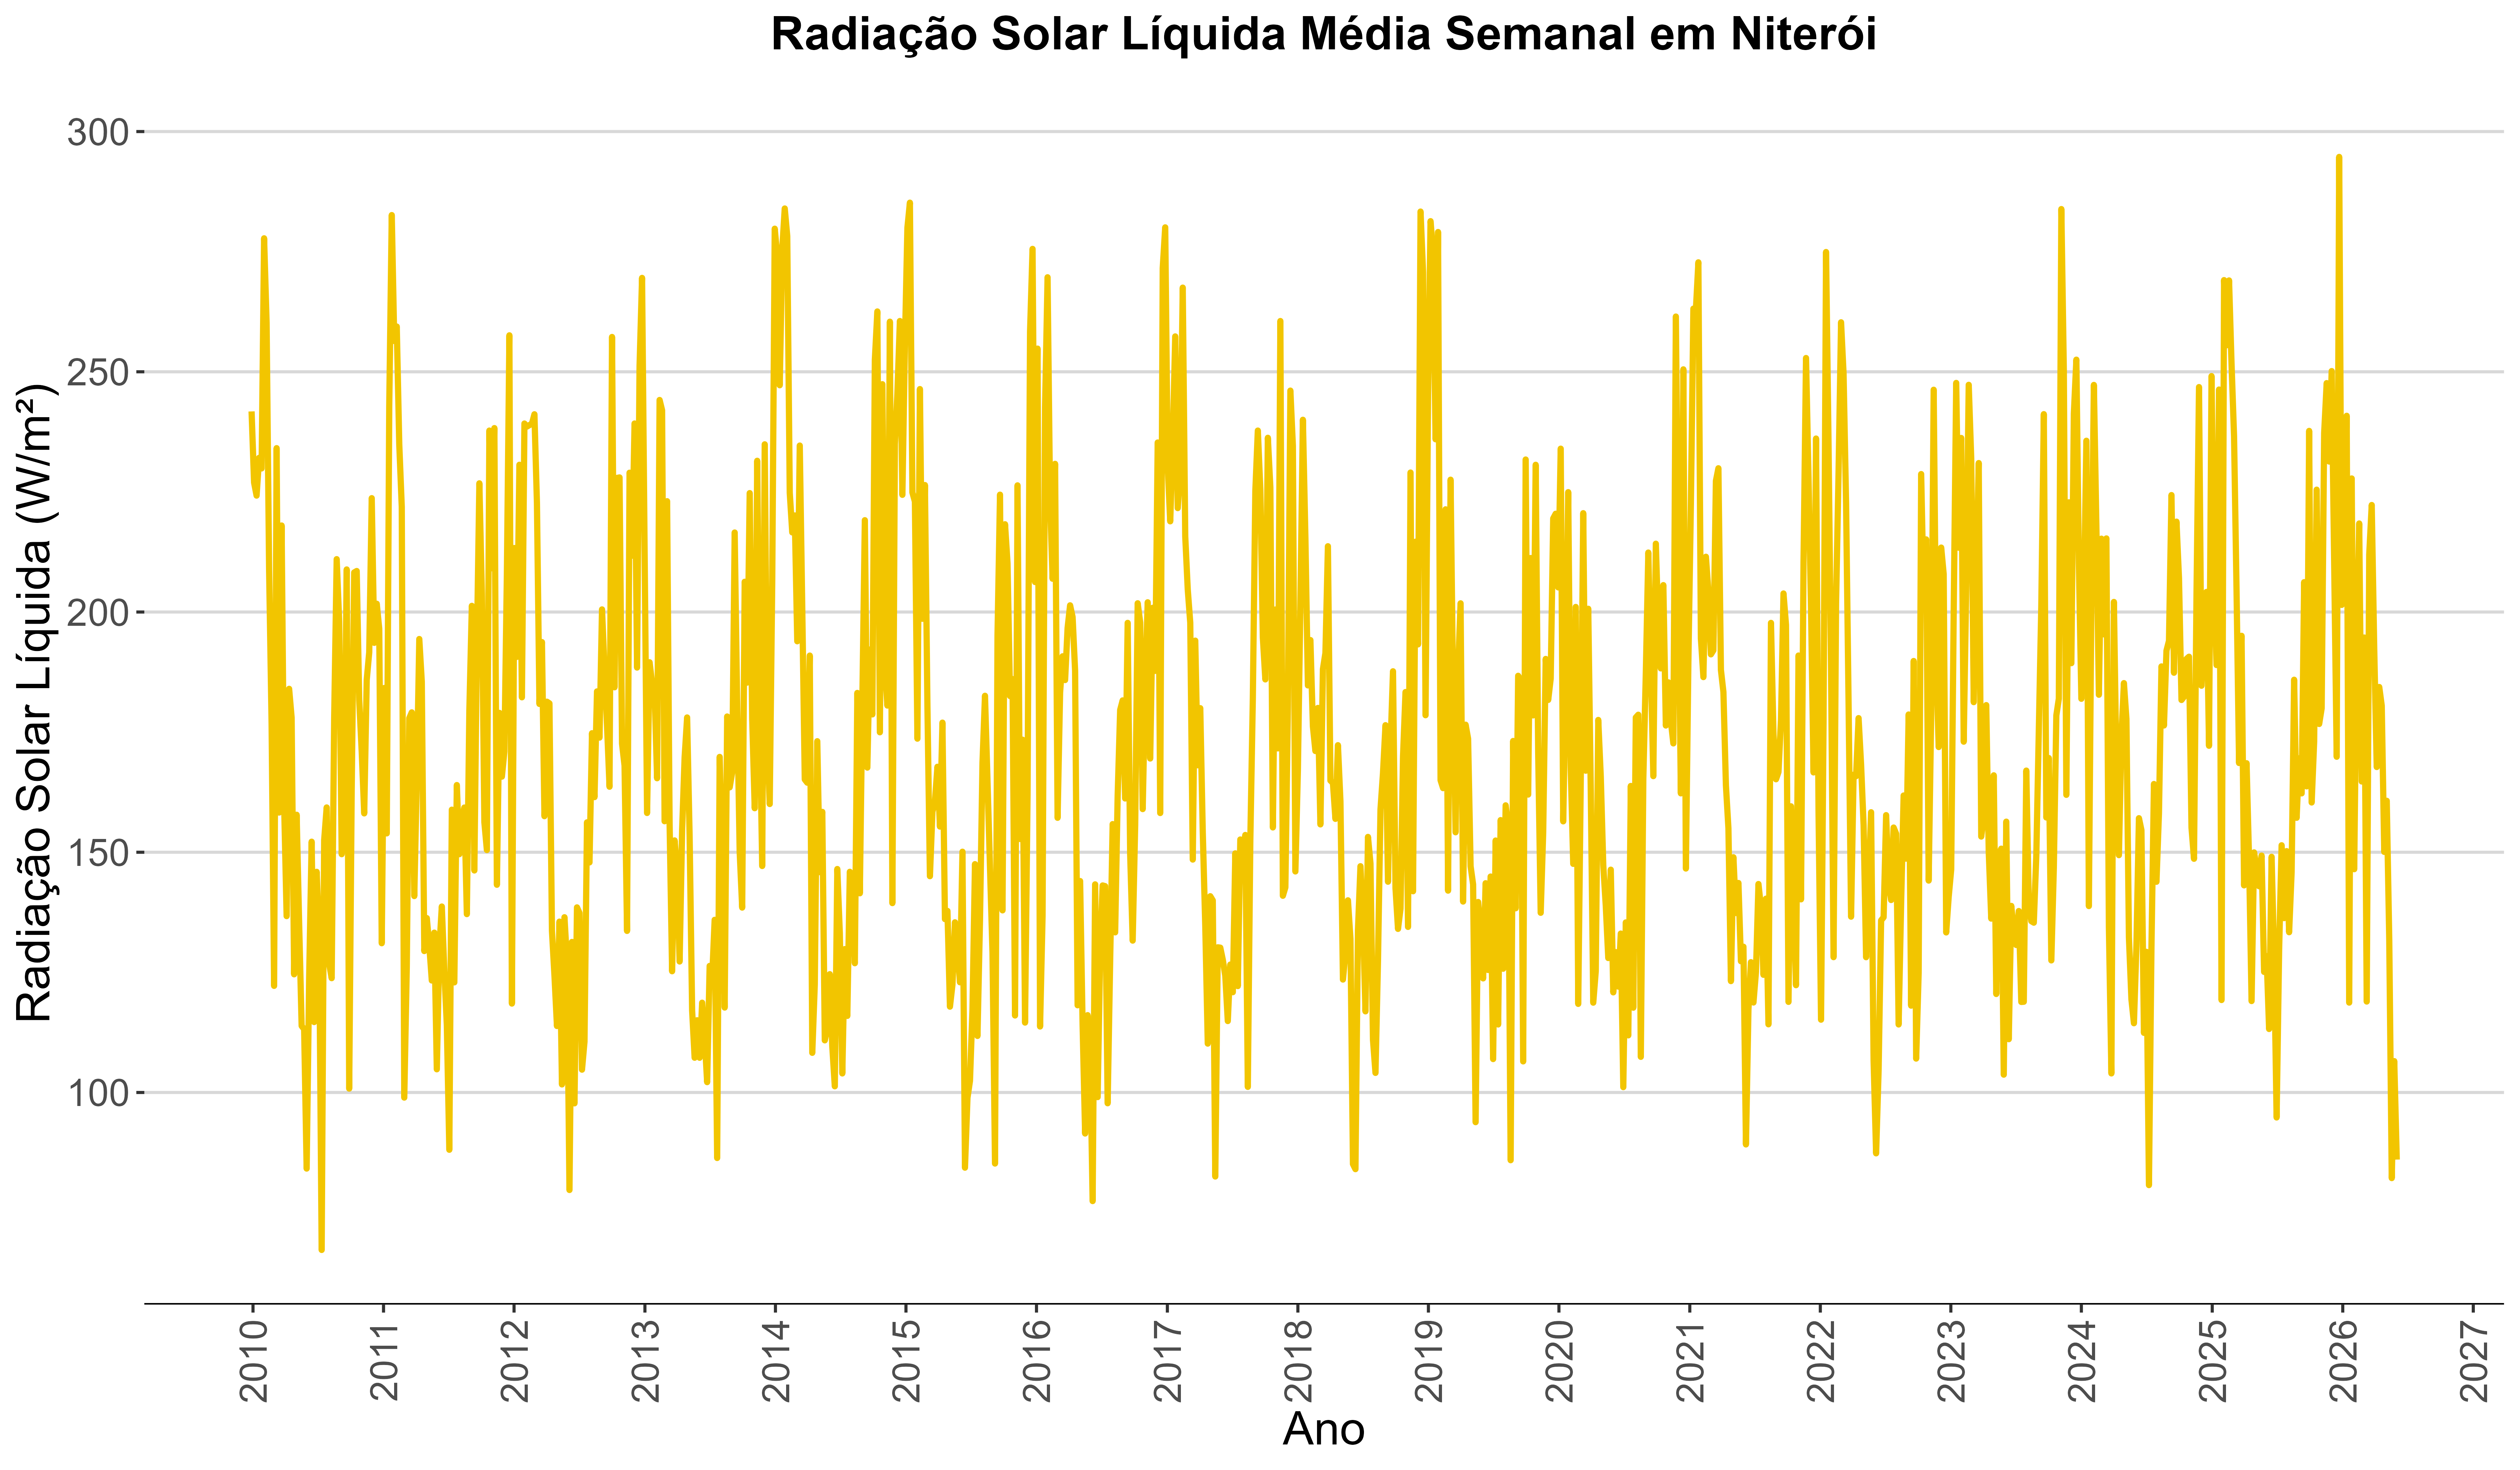
\includegraphics[keepaspectratio]{resultados/RadiacaoSolar/02_radiacaosolar_semanal.png}}

}

\caption{Radiação Solar Líquida Média Semanal}

\end{figure}%

\begin{figure}[H]

{\centering \pandocbounded{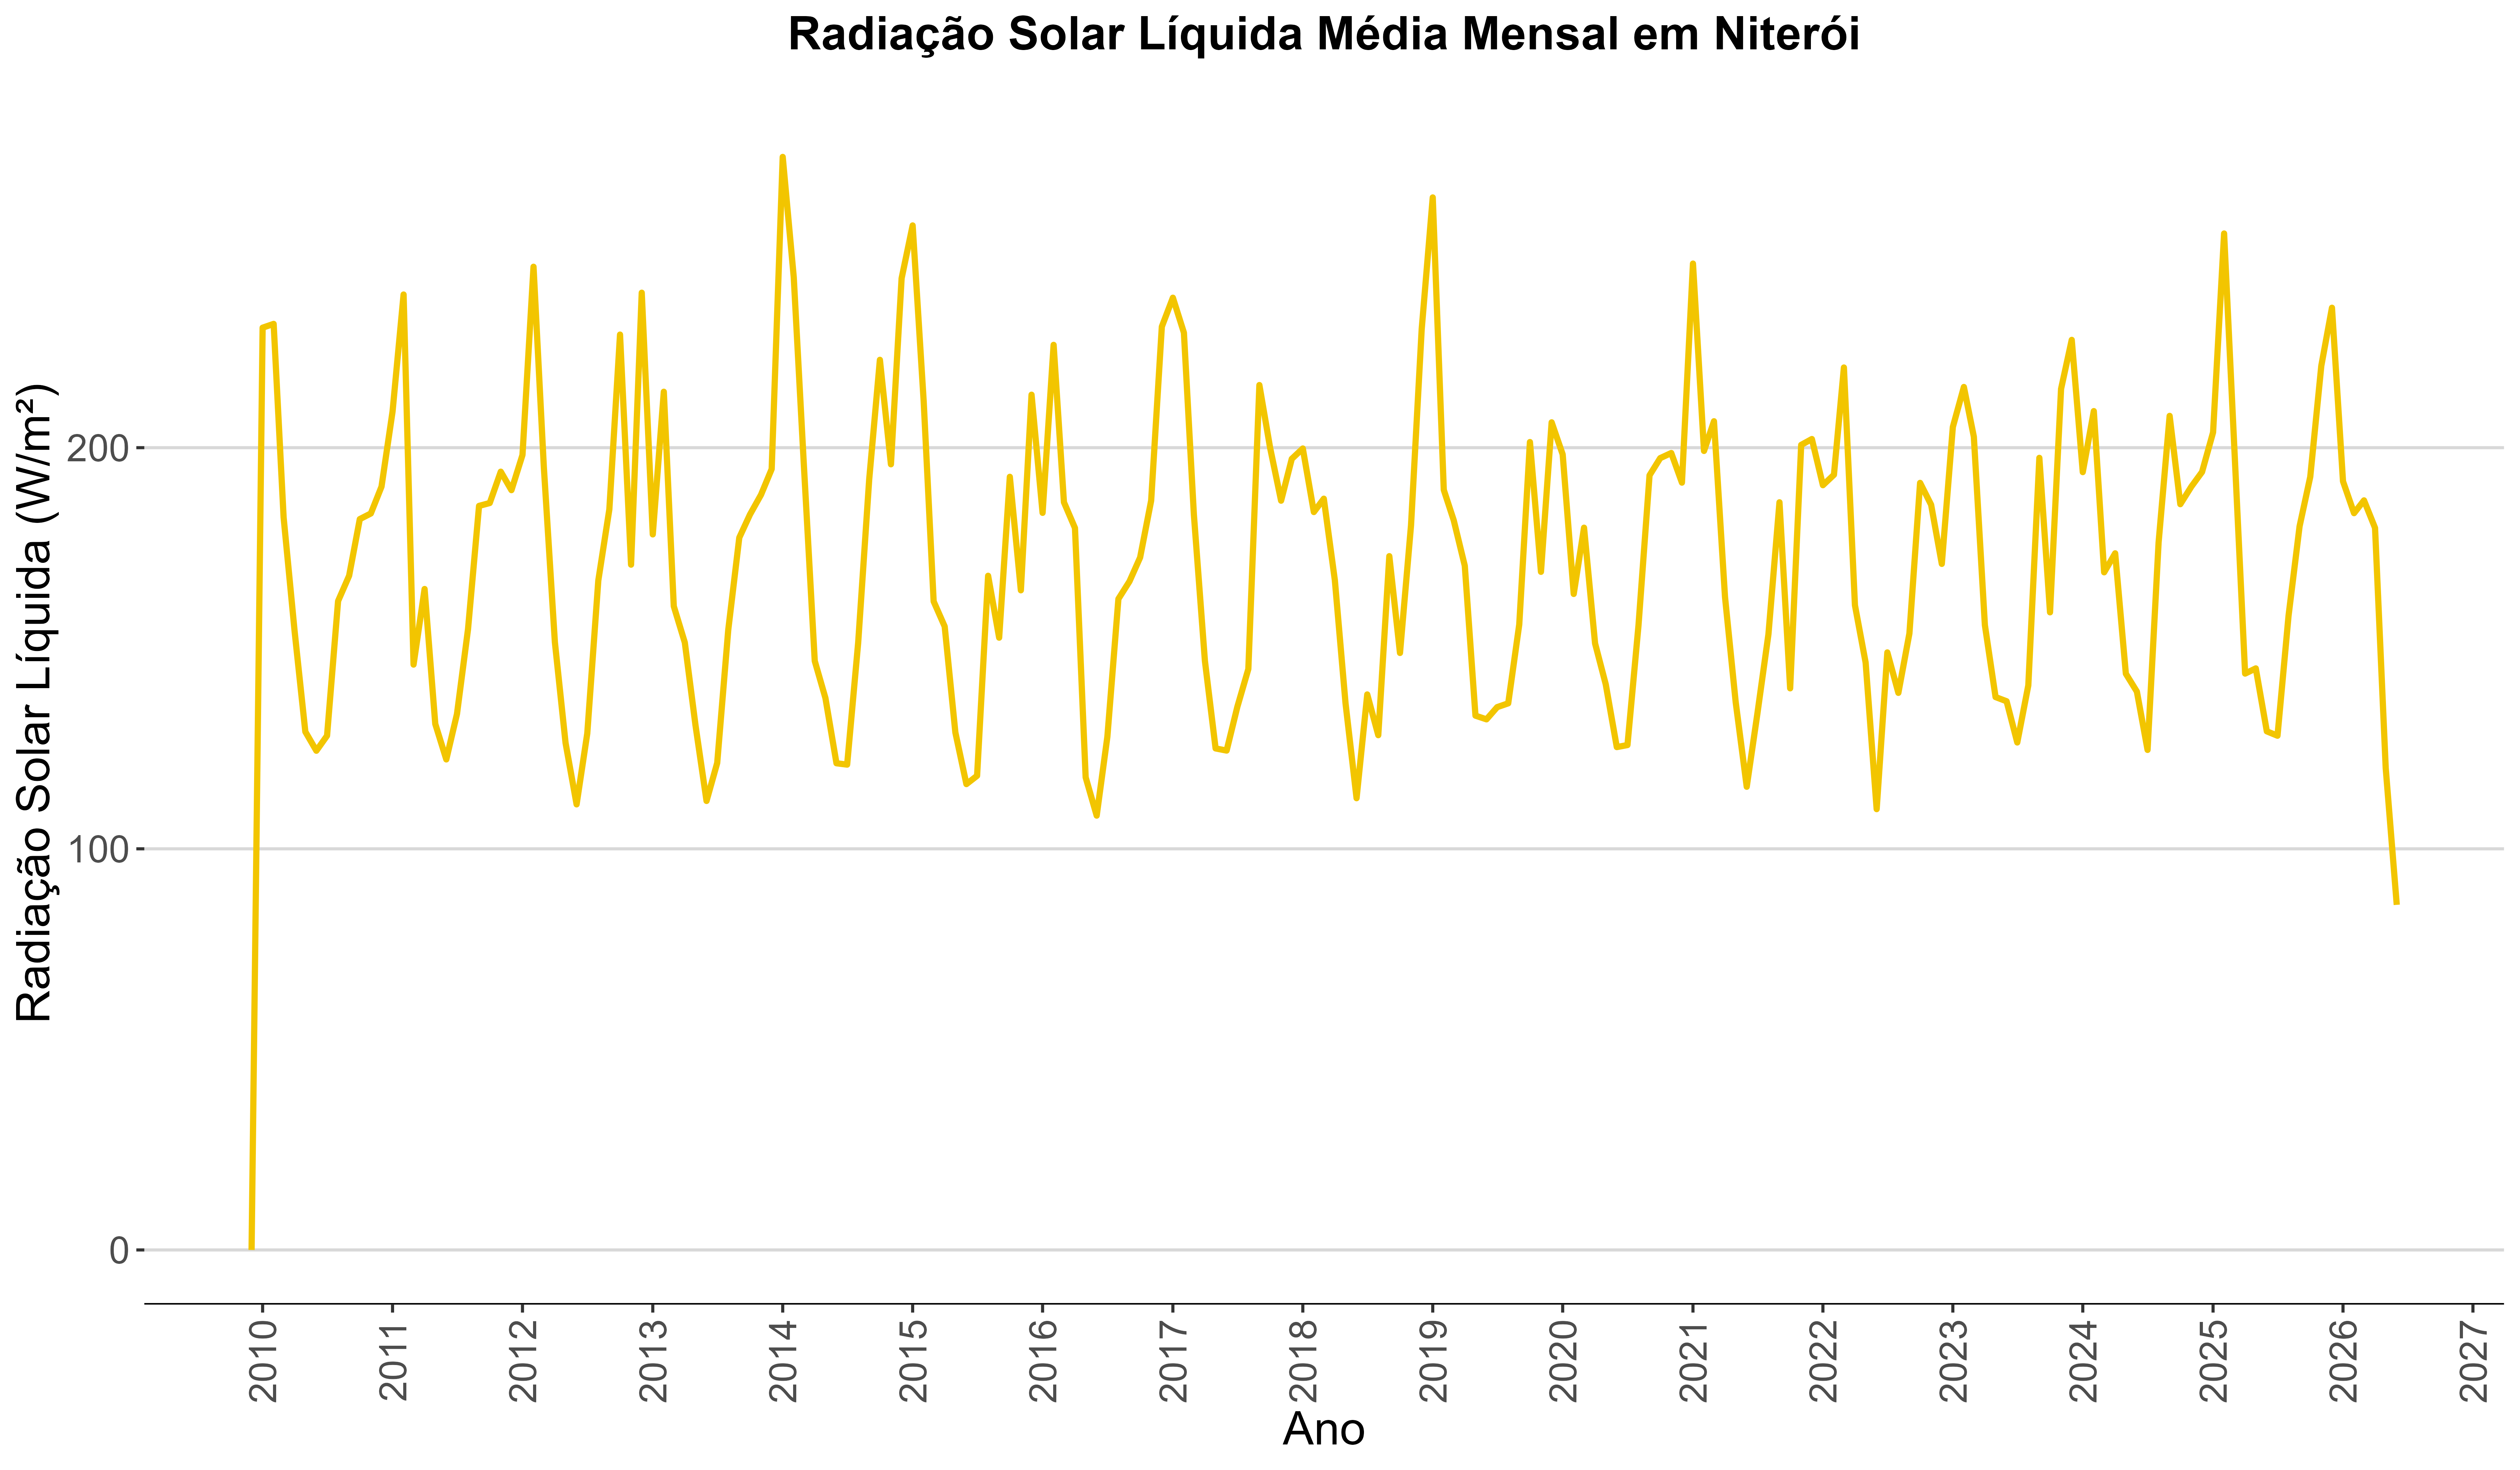
\includegraphics[keepaspectratio]{resultados/RadiacaoSolar/03_radiacaosolar_mensal.png}}

}

\caption{Radiação Solar Líquida Média Mensal}

\end{figure}%

\begin{figure}[H]

{\centering \pandocbounded{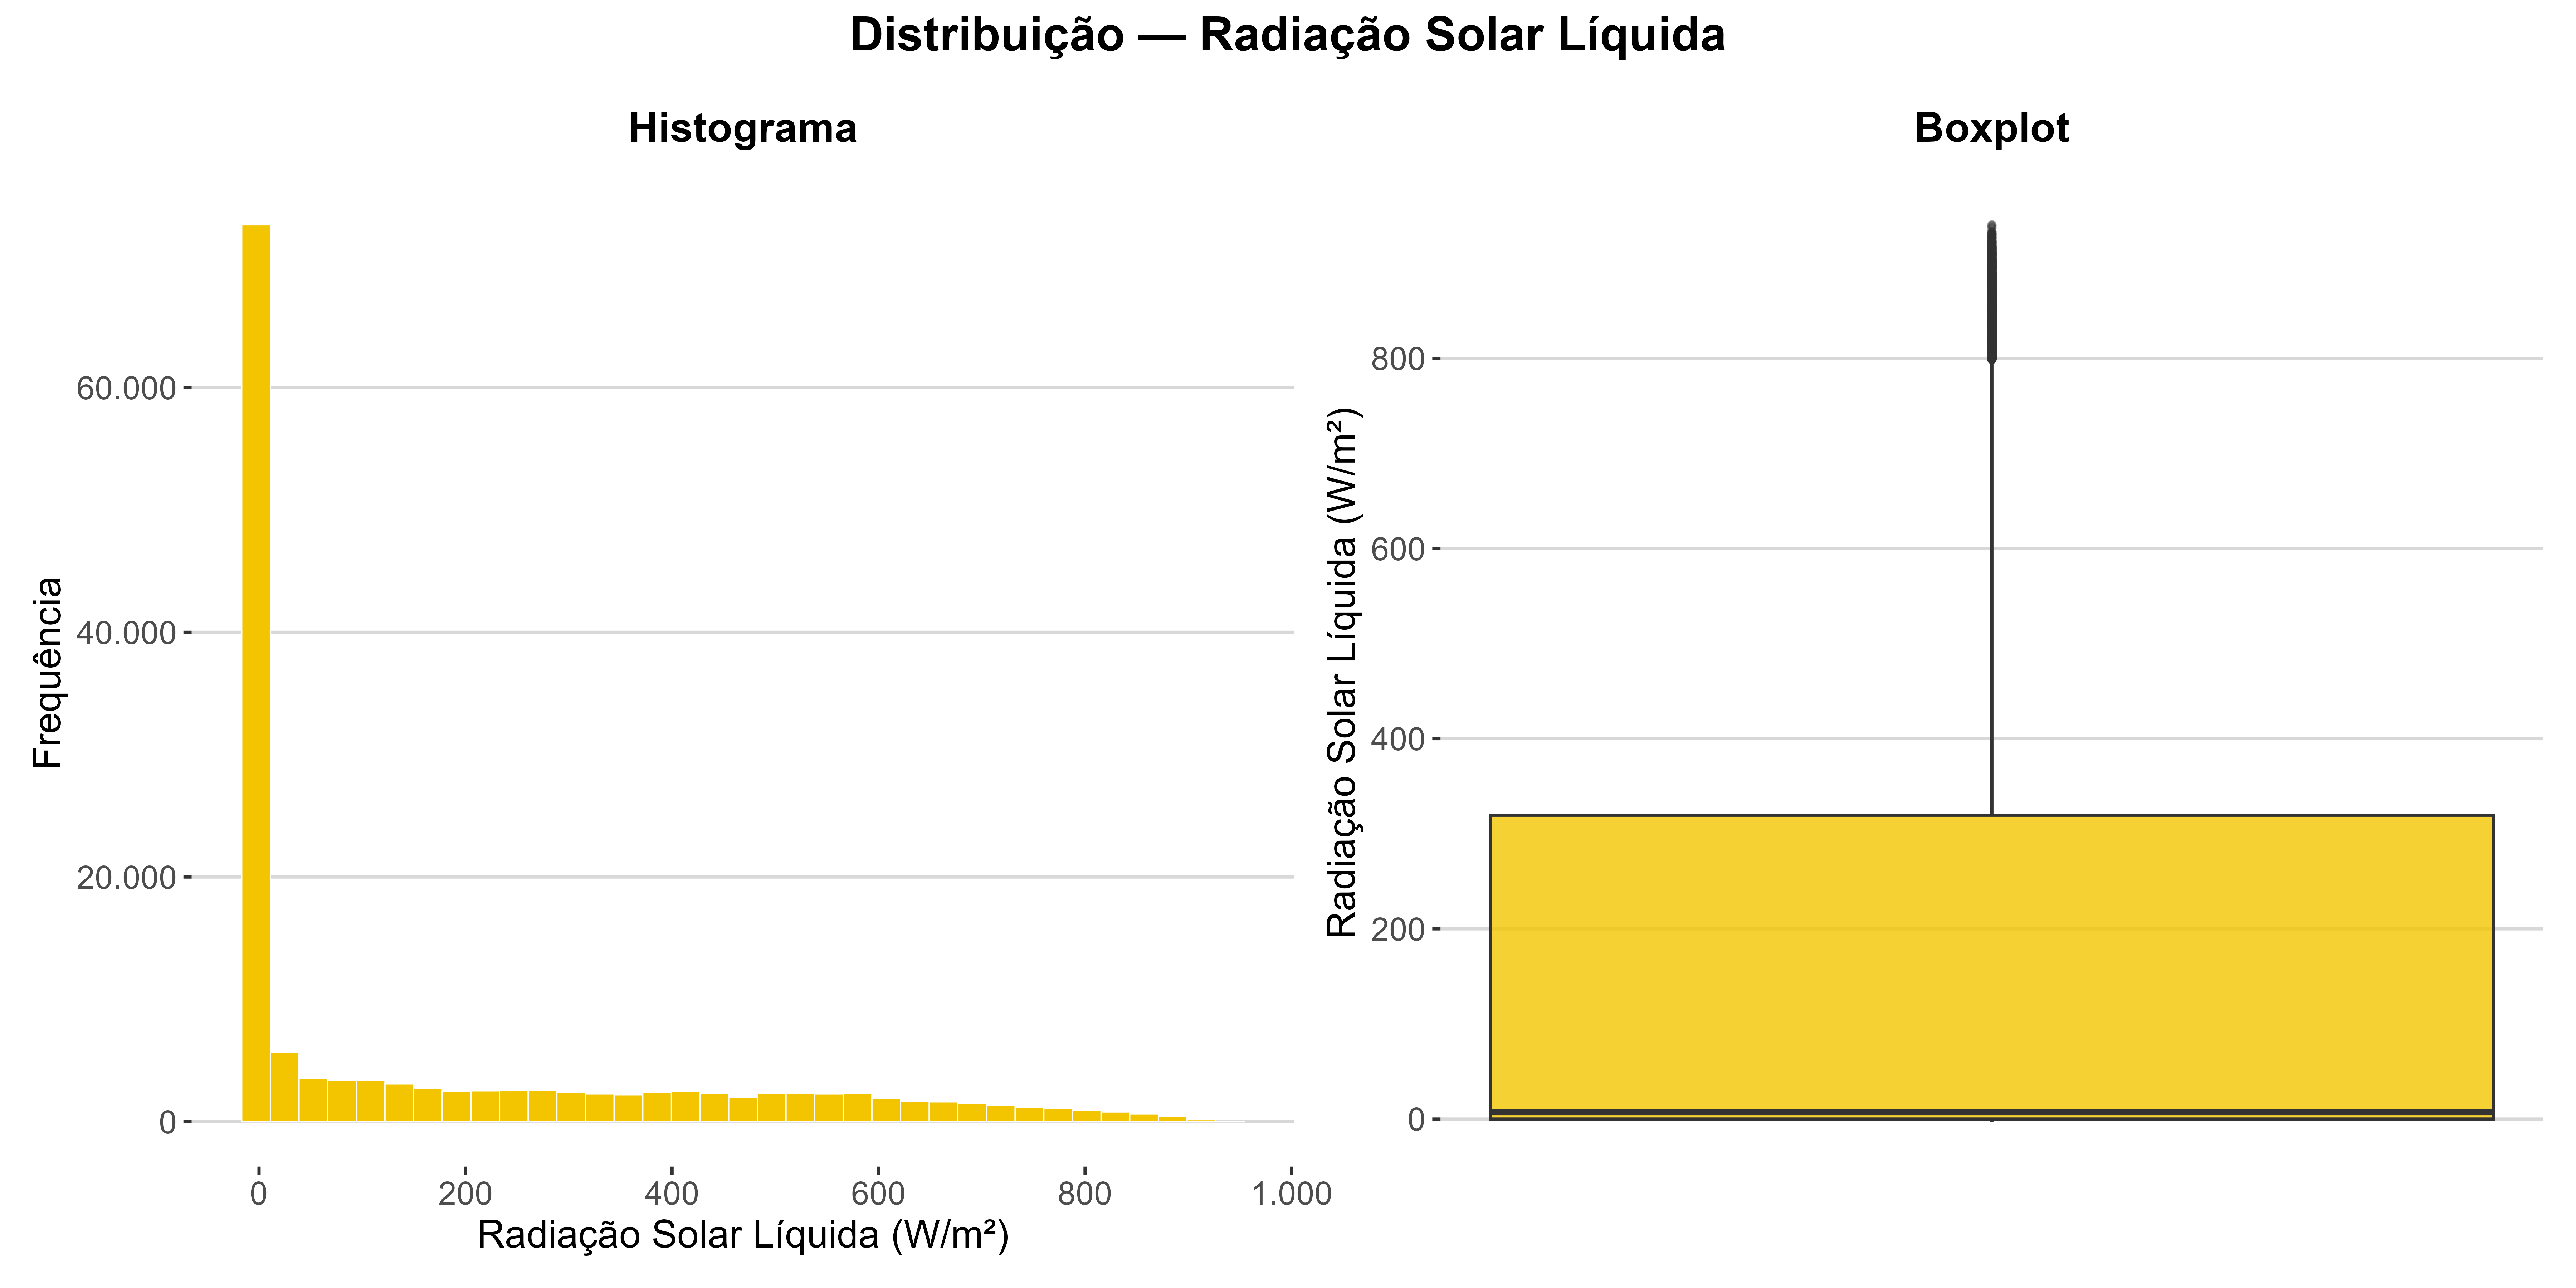
\includegraphics[keepaspectratio]{resultados/RadiacaoSolar/04_radiacaosolar_distribuicao.png}}

}

\caption{Distribuição da Radiação Solar Líquida}

\end{figure}%

\paragraph{Principais Achados}\label{principais-achados-6}

A radiação solar líquida exibe a \textbf{mais marcante sazonalidade
diária} de todas as variáveis: os valores são positivos durante o dia e
nulos (ou levemente negativos) à noite, gerando uma estrutura periódica
de 24 horas extremamente regular. Na escala diária, os picos chegam a
valores superiores a 200 W/m² no verão, enquanto o inverno apresenta
médias diárias claramente menores.

A distribuição é \textbf{assimétrica à direita,} com pico no zero.

\subsubsection{Radiação Térmica
Líquida}\label{radiauxe7uxe3o-tuxe9rmica-luxedquida}

\begin{figure}[H]

{\centering \pandocbounded{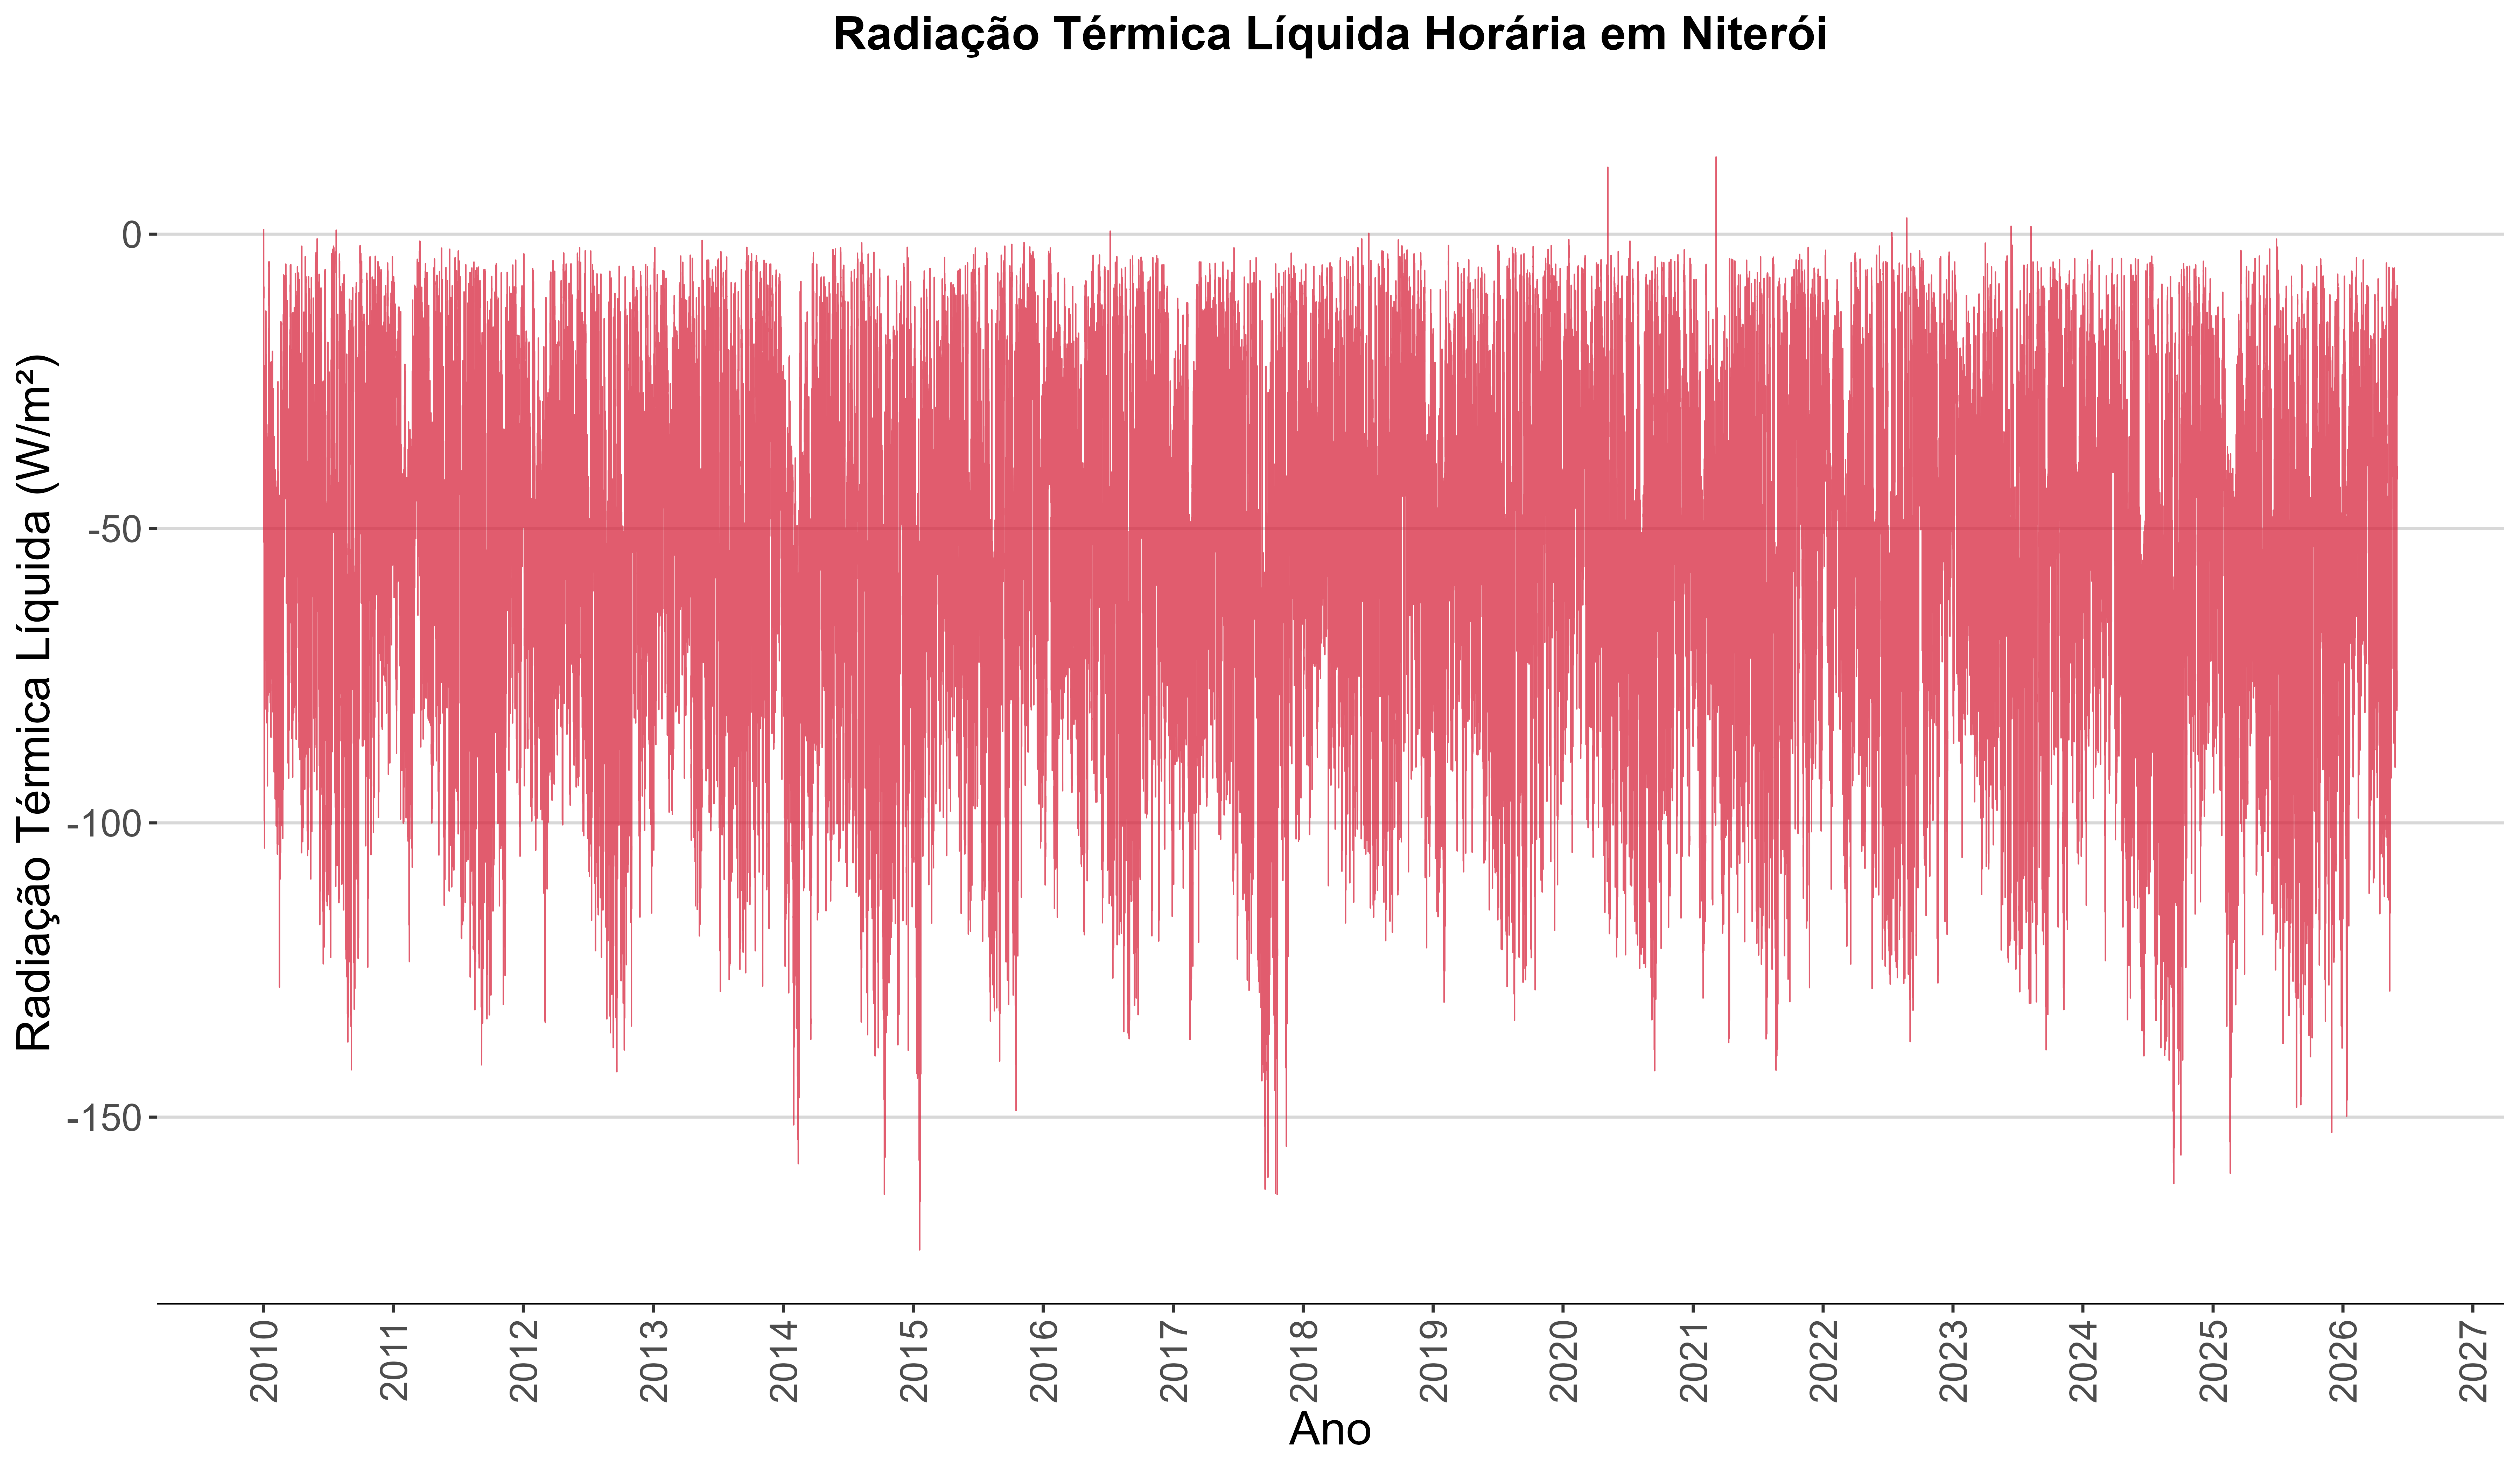
\includegraphics[keepaspectratio]{resultados/RadiacaoTermica/00_radiacaotermica_horario.png}}

}

\caption{Radiação Térmica Líquida Horária}

\end{figure}%

\begin{figure}[H]

{\centering \pandocbounded{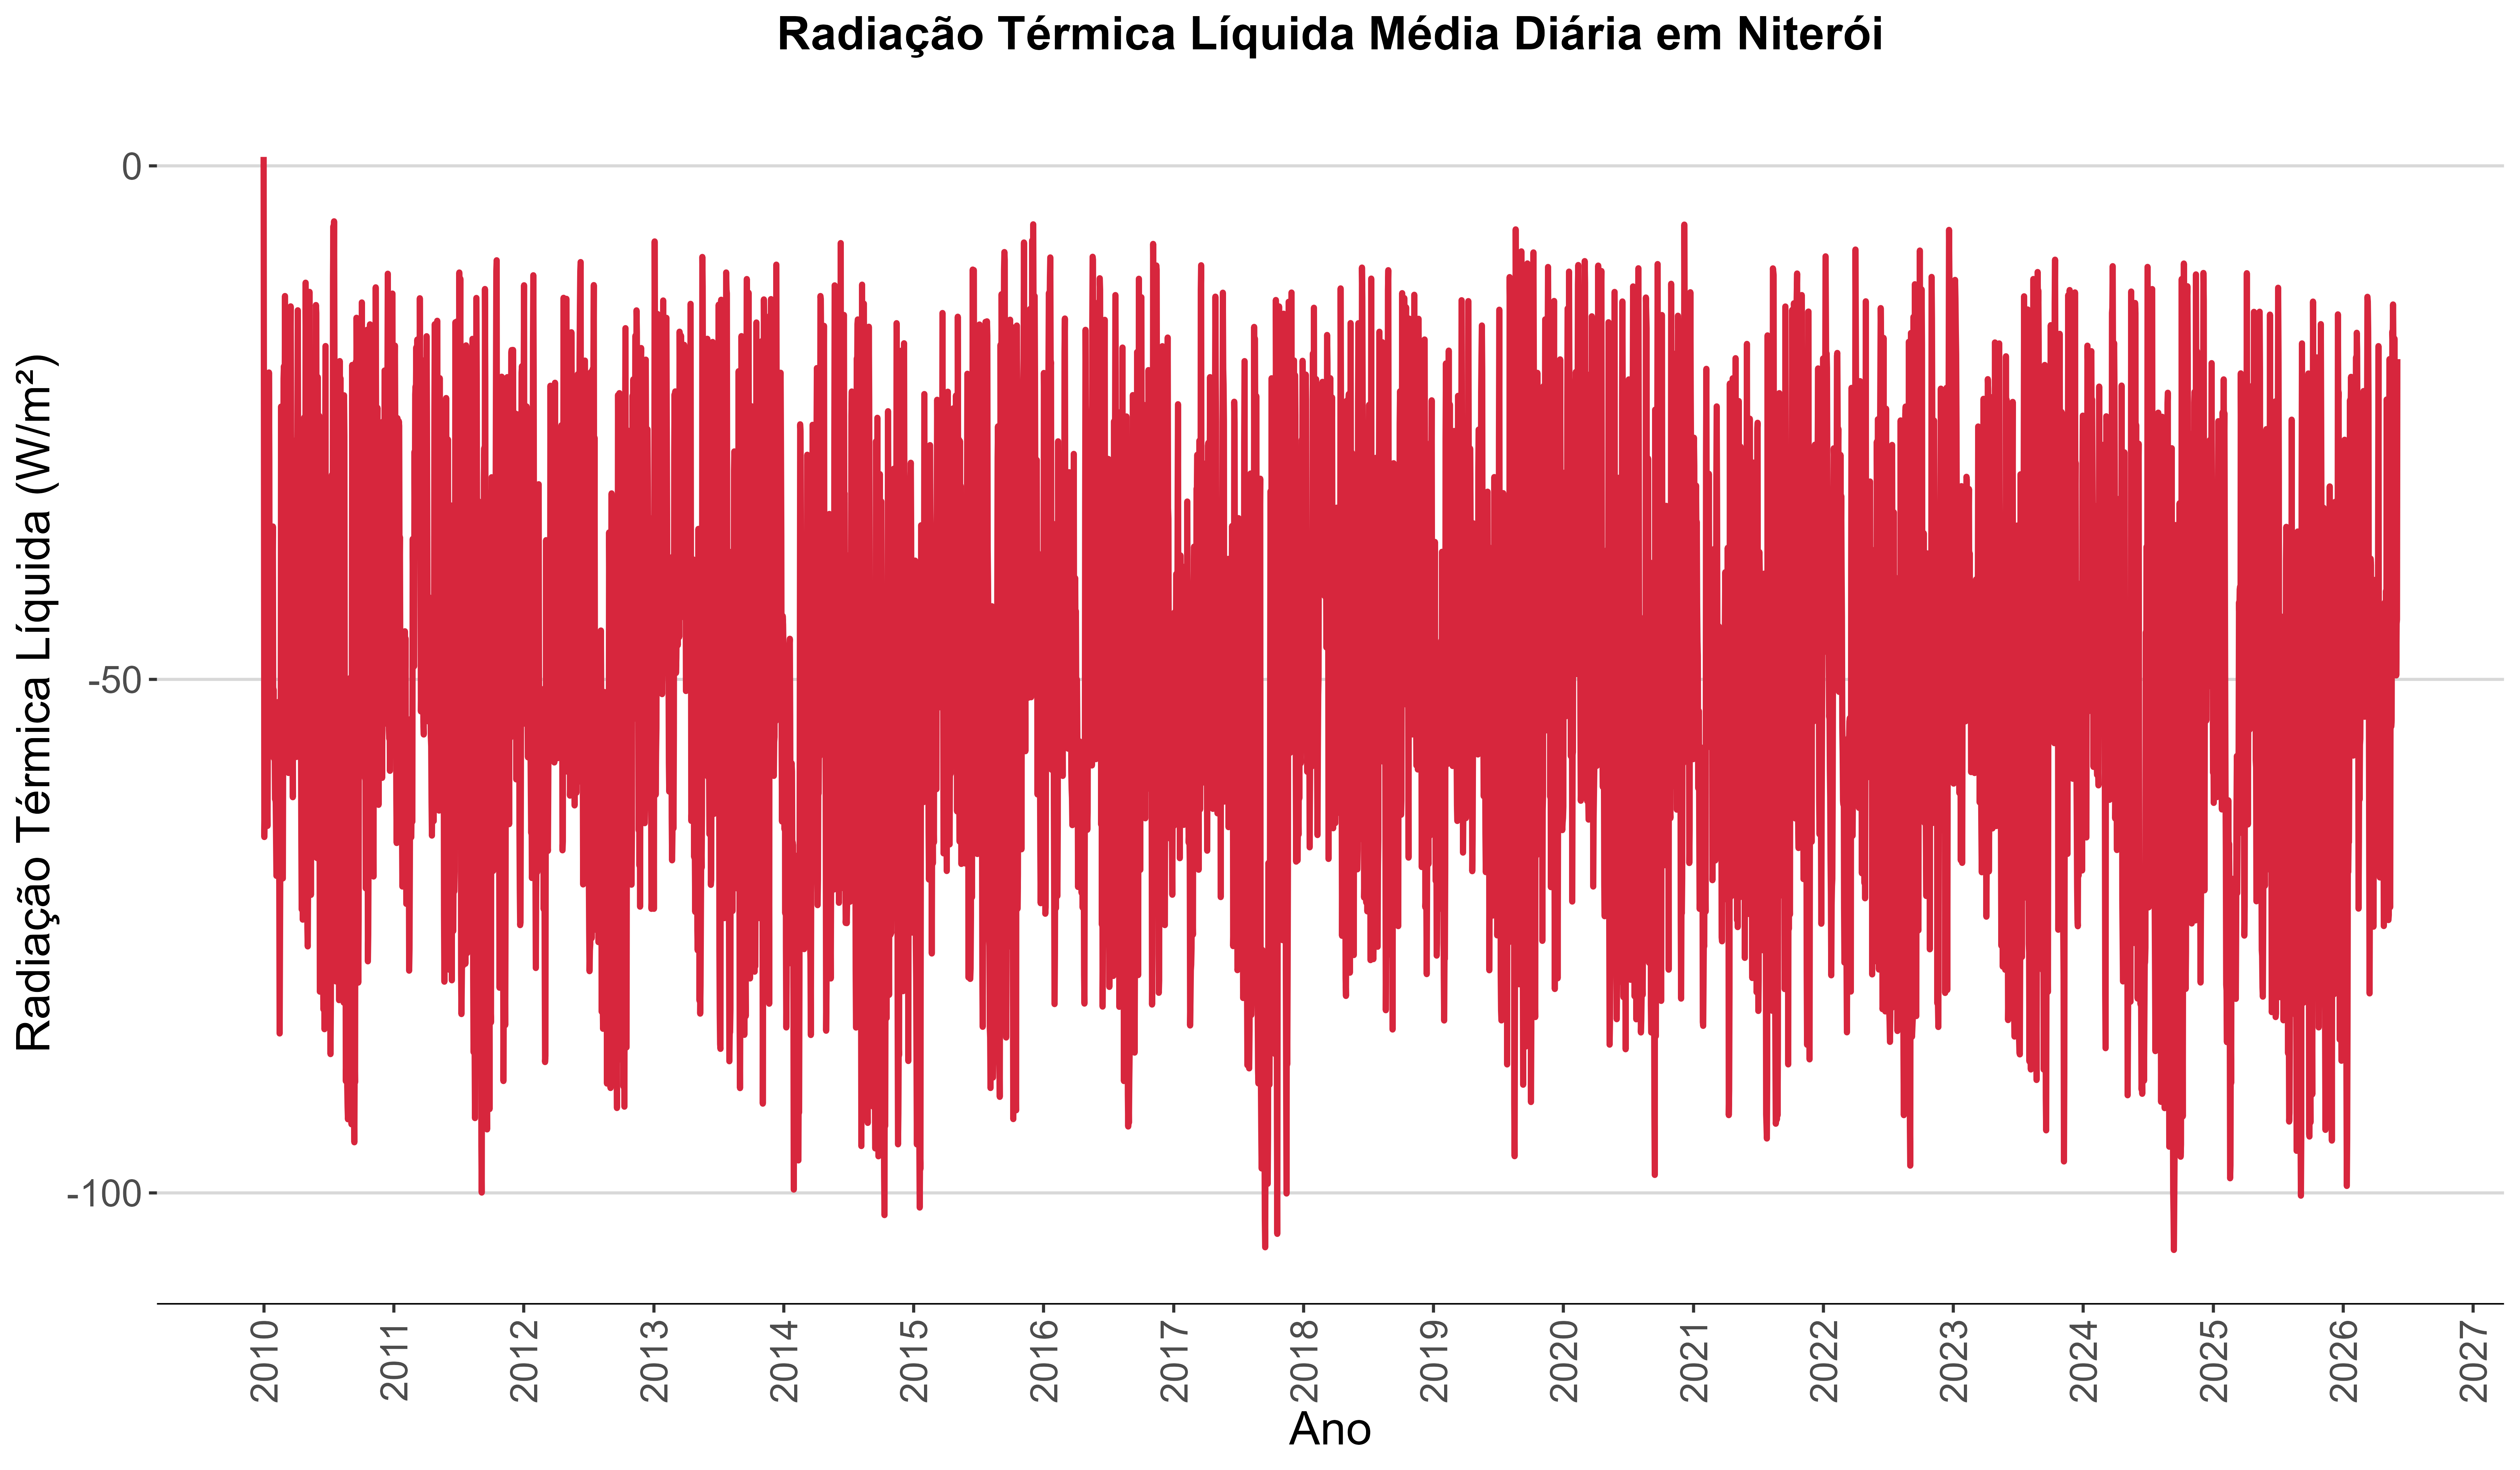
\includegraphics[keepaspectratio]{resultados/RadiacaoTermica/01_radiacaotermica_diario.png}}

}

\caption{Radiação Térmica Líquida Média Diária}

\end{figure}%

\begin{figure}[H]

{\centering \pandocbounded{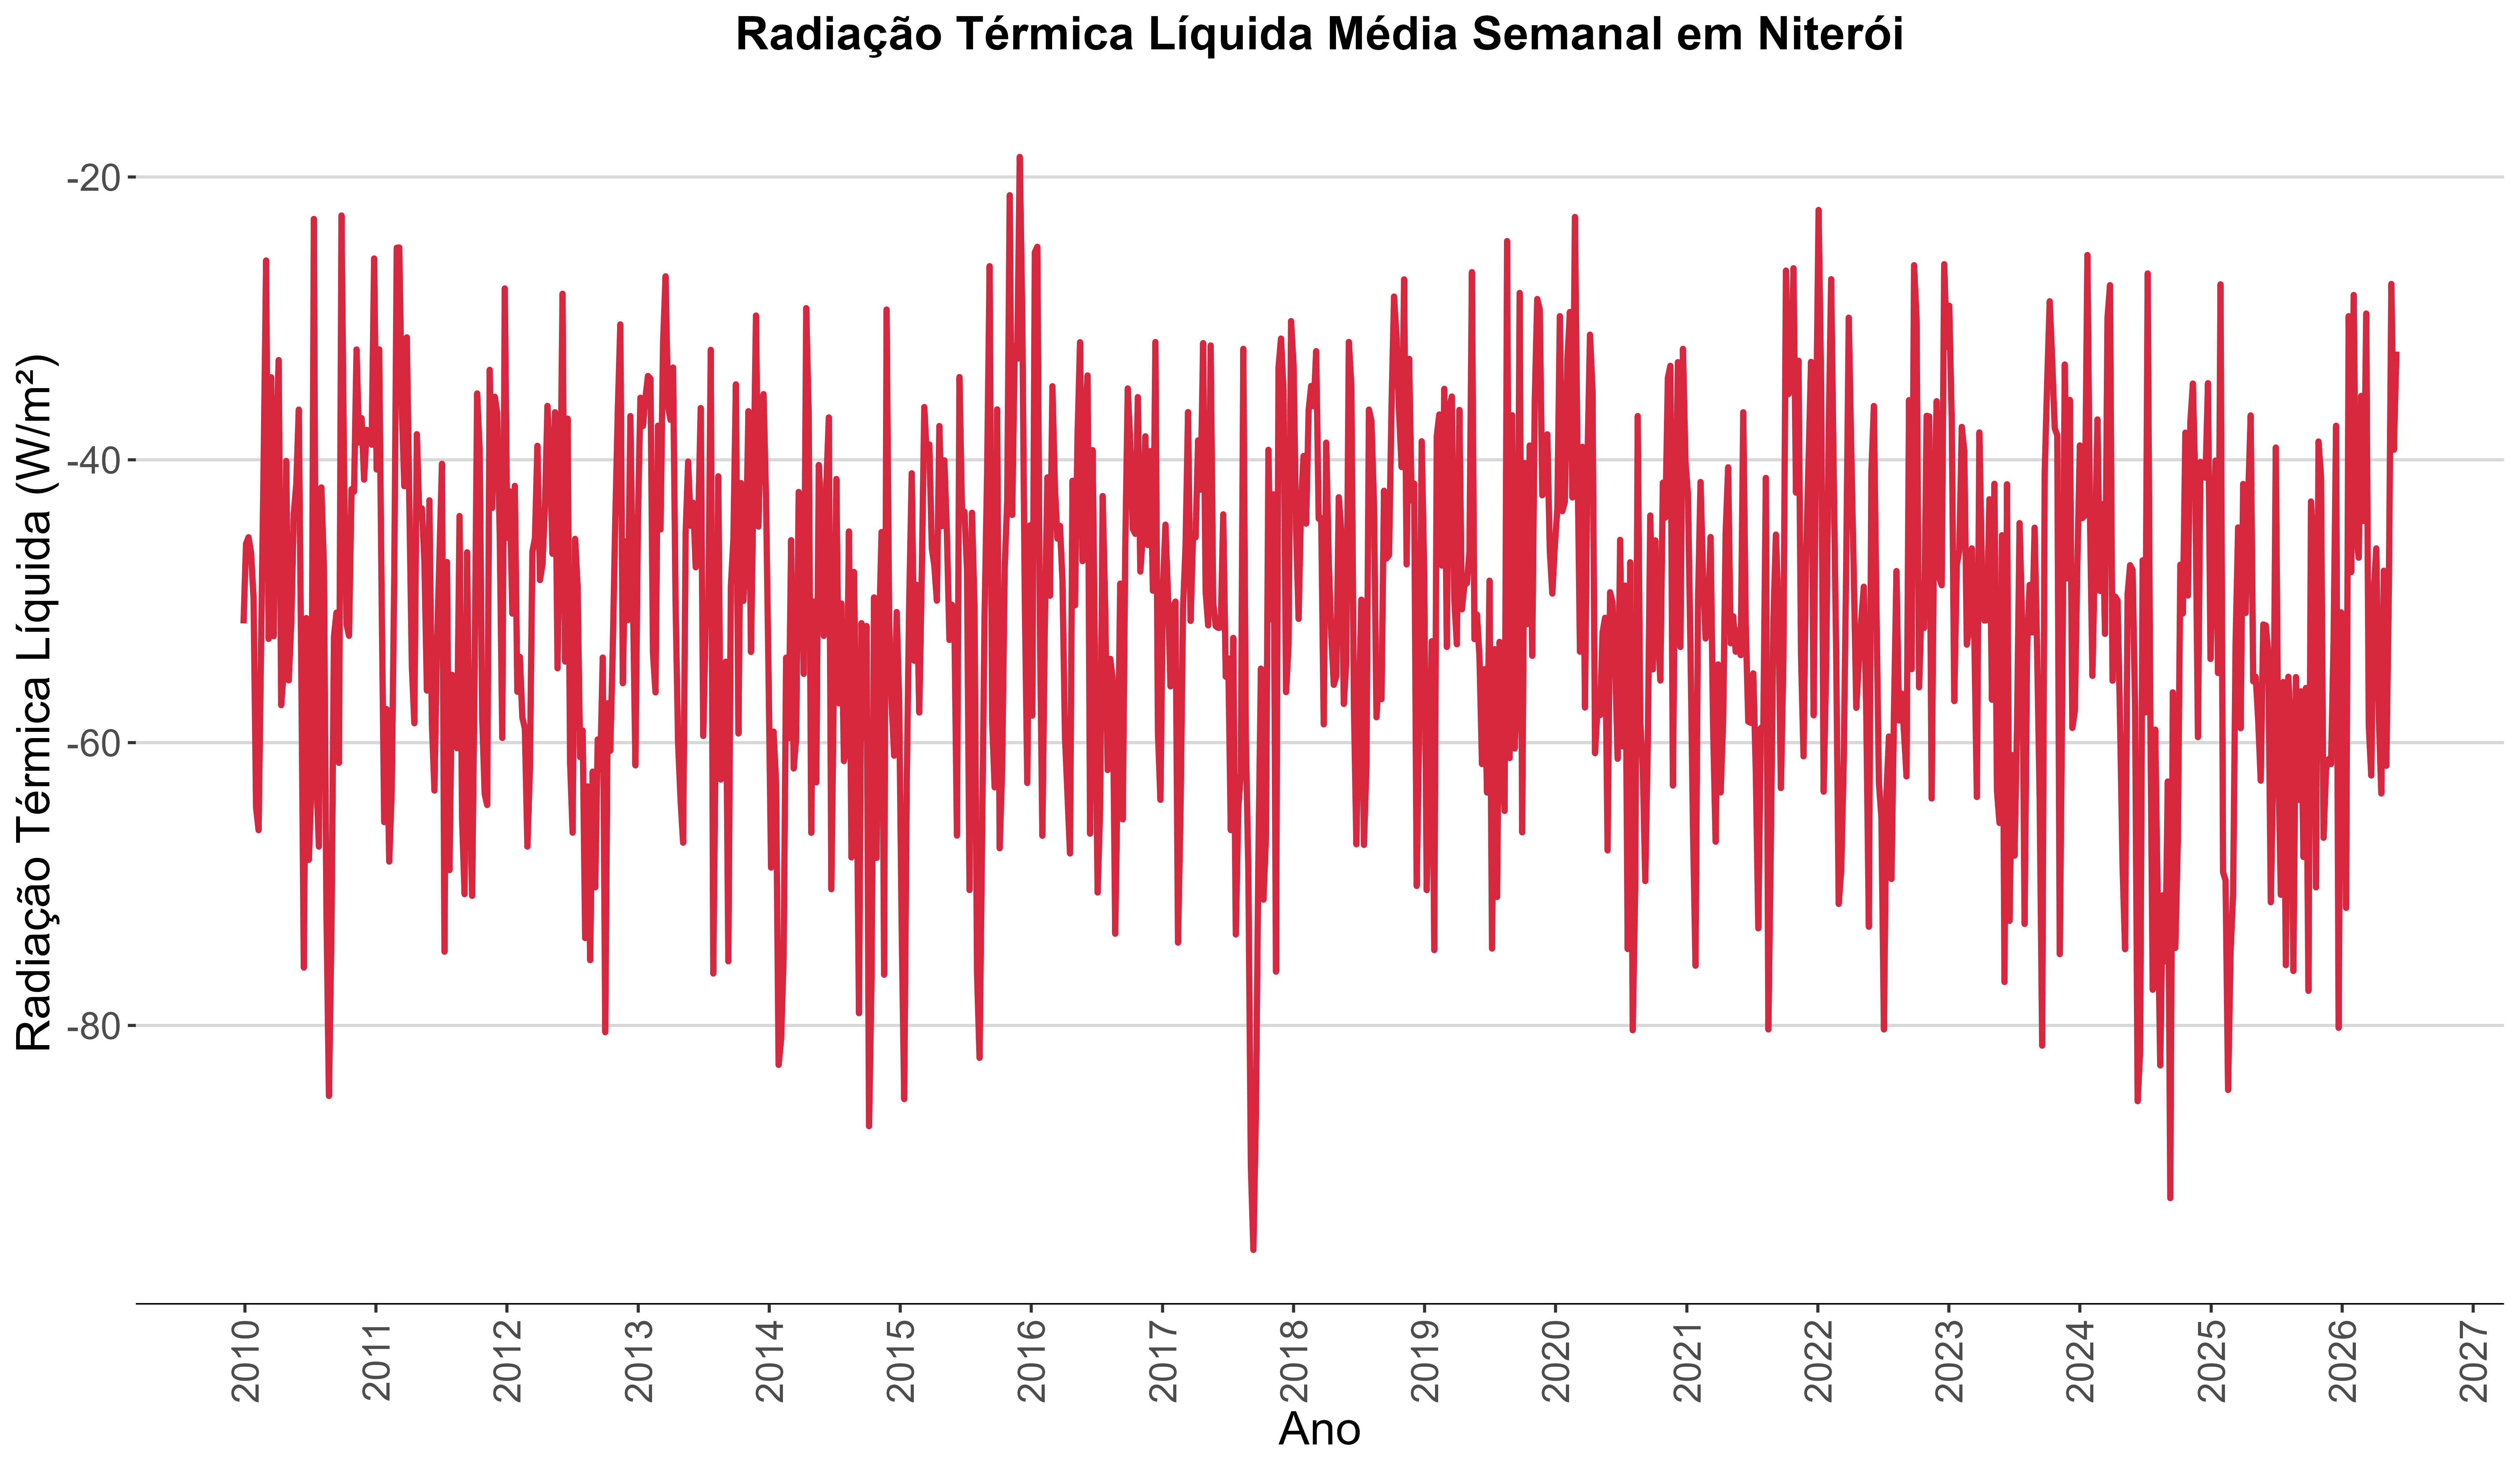
\includegraphics[keepaspectratio]{resultados/RadiacaoTermica/02_radiacaotermica_semanal.png}}

}

\caption{Radiação Térmica Líquida Média Semanal}

\end{figure}%

\begin{figure}[H]

{\centering \pandocbounded{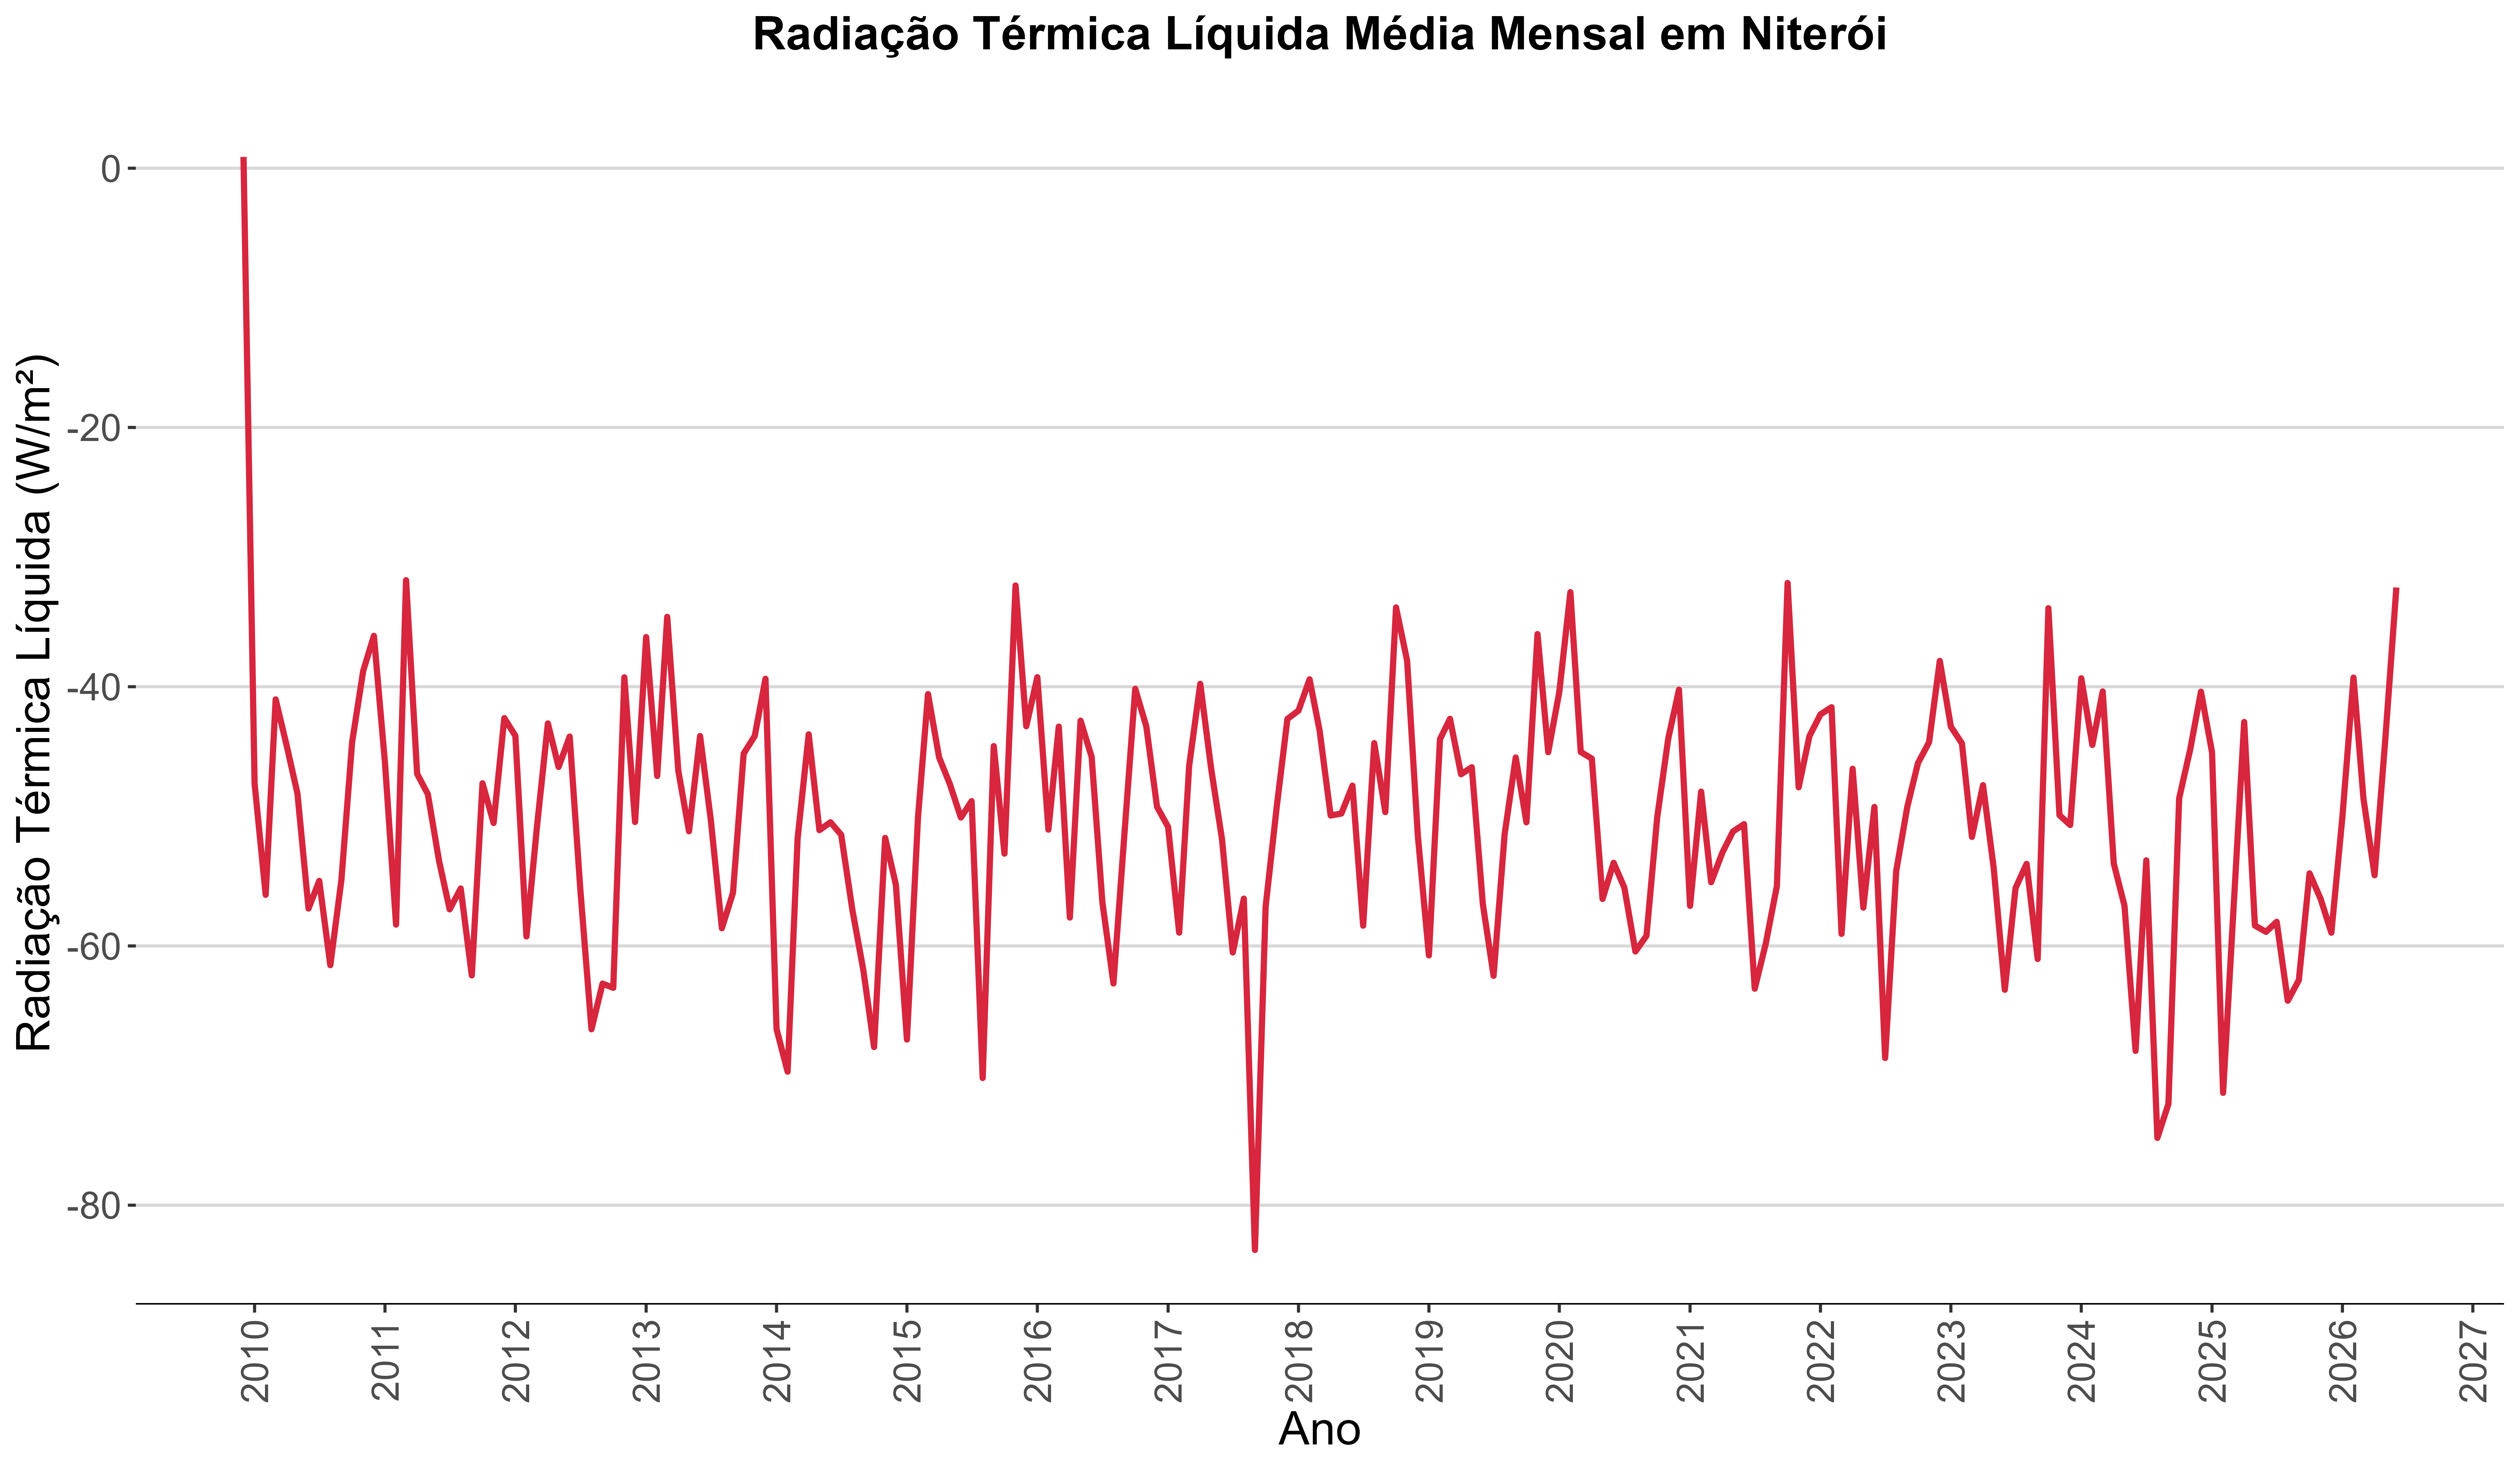
\includegraphics[keepaspectratio]{resultados/RadiacaoTermica/03_radiacaotermica_mensal.png}}

}

\caption{Radiação Térmica Líquida Média Mensal}

\end{figure}%

\begin{figure}[H]

{\centering \pandocbounded{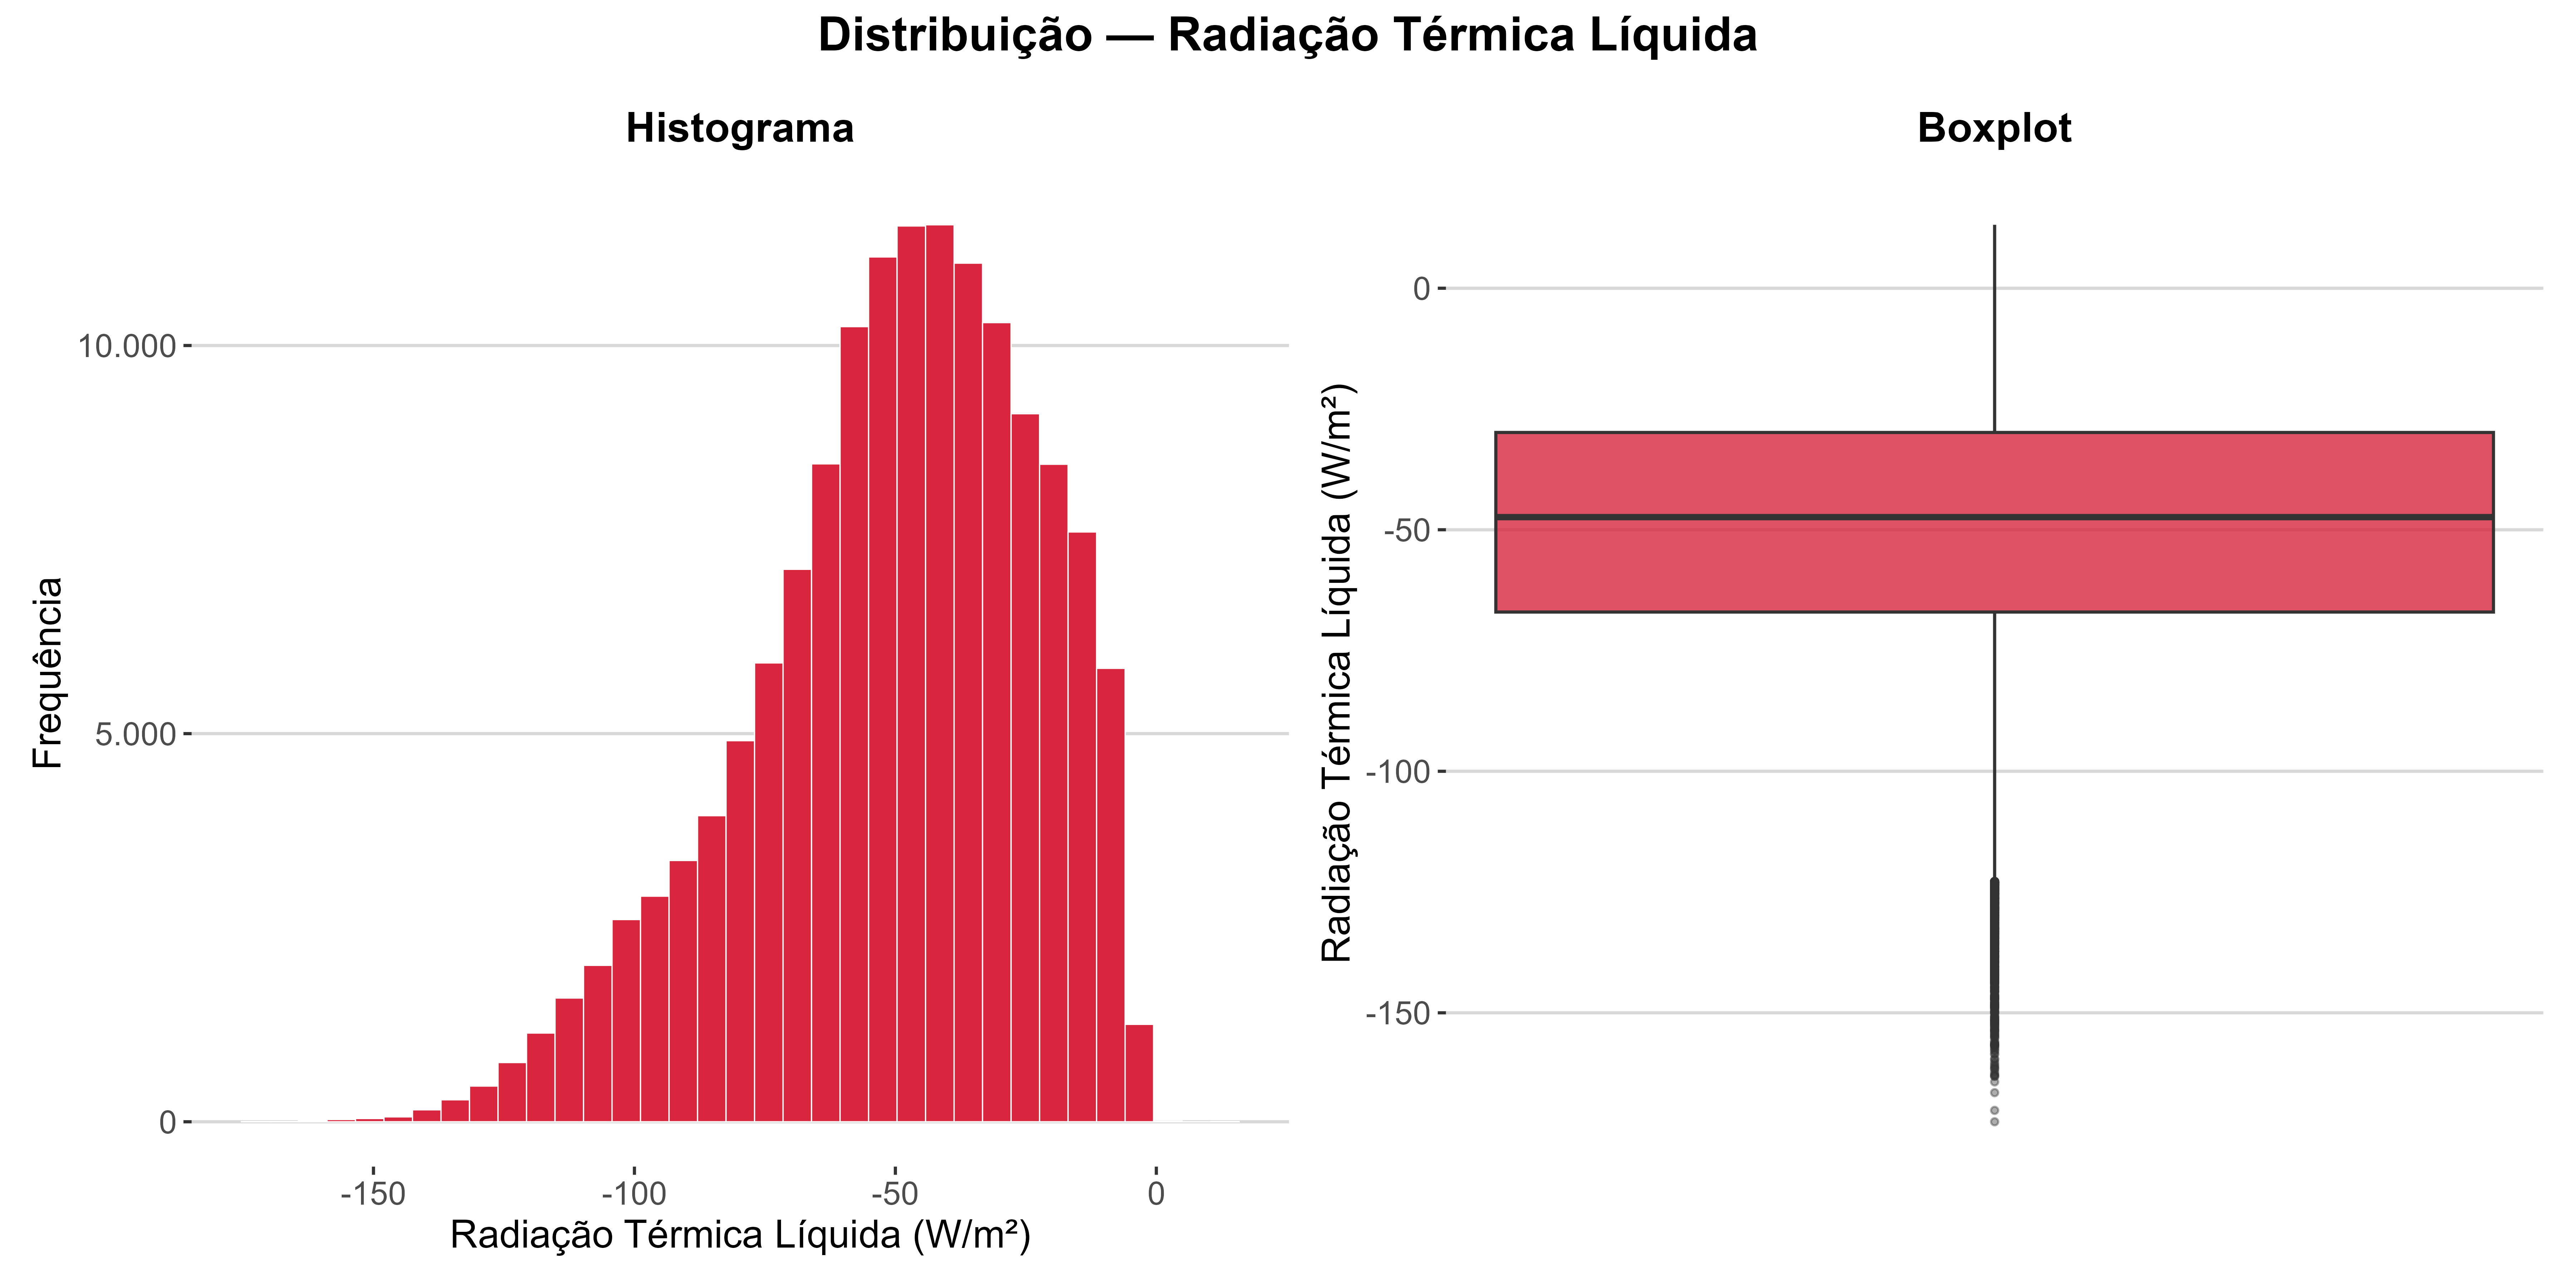
\includegraphics[keepaspectratio]{resultados/RadiacaoTermica/04_radiacaotermica_distribuicao.png}}

}

\caption{Distribuição da Radiação Térmica Líquida}

\end{figure}%

\paragraph{Principais Achados}\label{principais-achados-7}

A radiação térmica líquida apresenta \textbf{valores negativos},
indicando perda contínua de energia pela superfície. A amplitude é menor
do que a da radiação solar, com variações sazonais moderadas e picos
negativos mais intensos no inverno (noites frias e céu limpo favorecem
maior perda radiativa).

A distribuição não tem caudas extremas pronunciadas como da radiação
solar.

\subsubsection{Fluxo de Calor
Sensível}\label{fluxo-de-calor-sensuxedvel}

\begin{figure}[H]

{\centering \pandocbounded{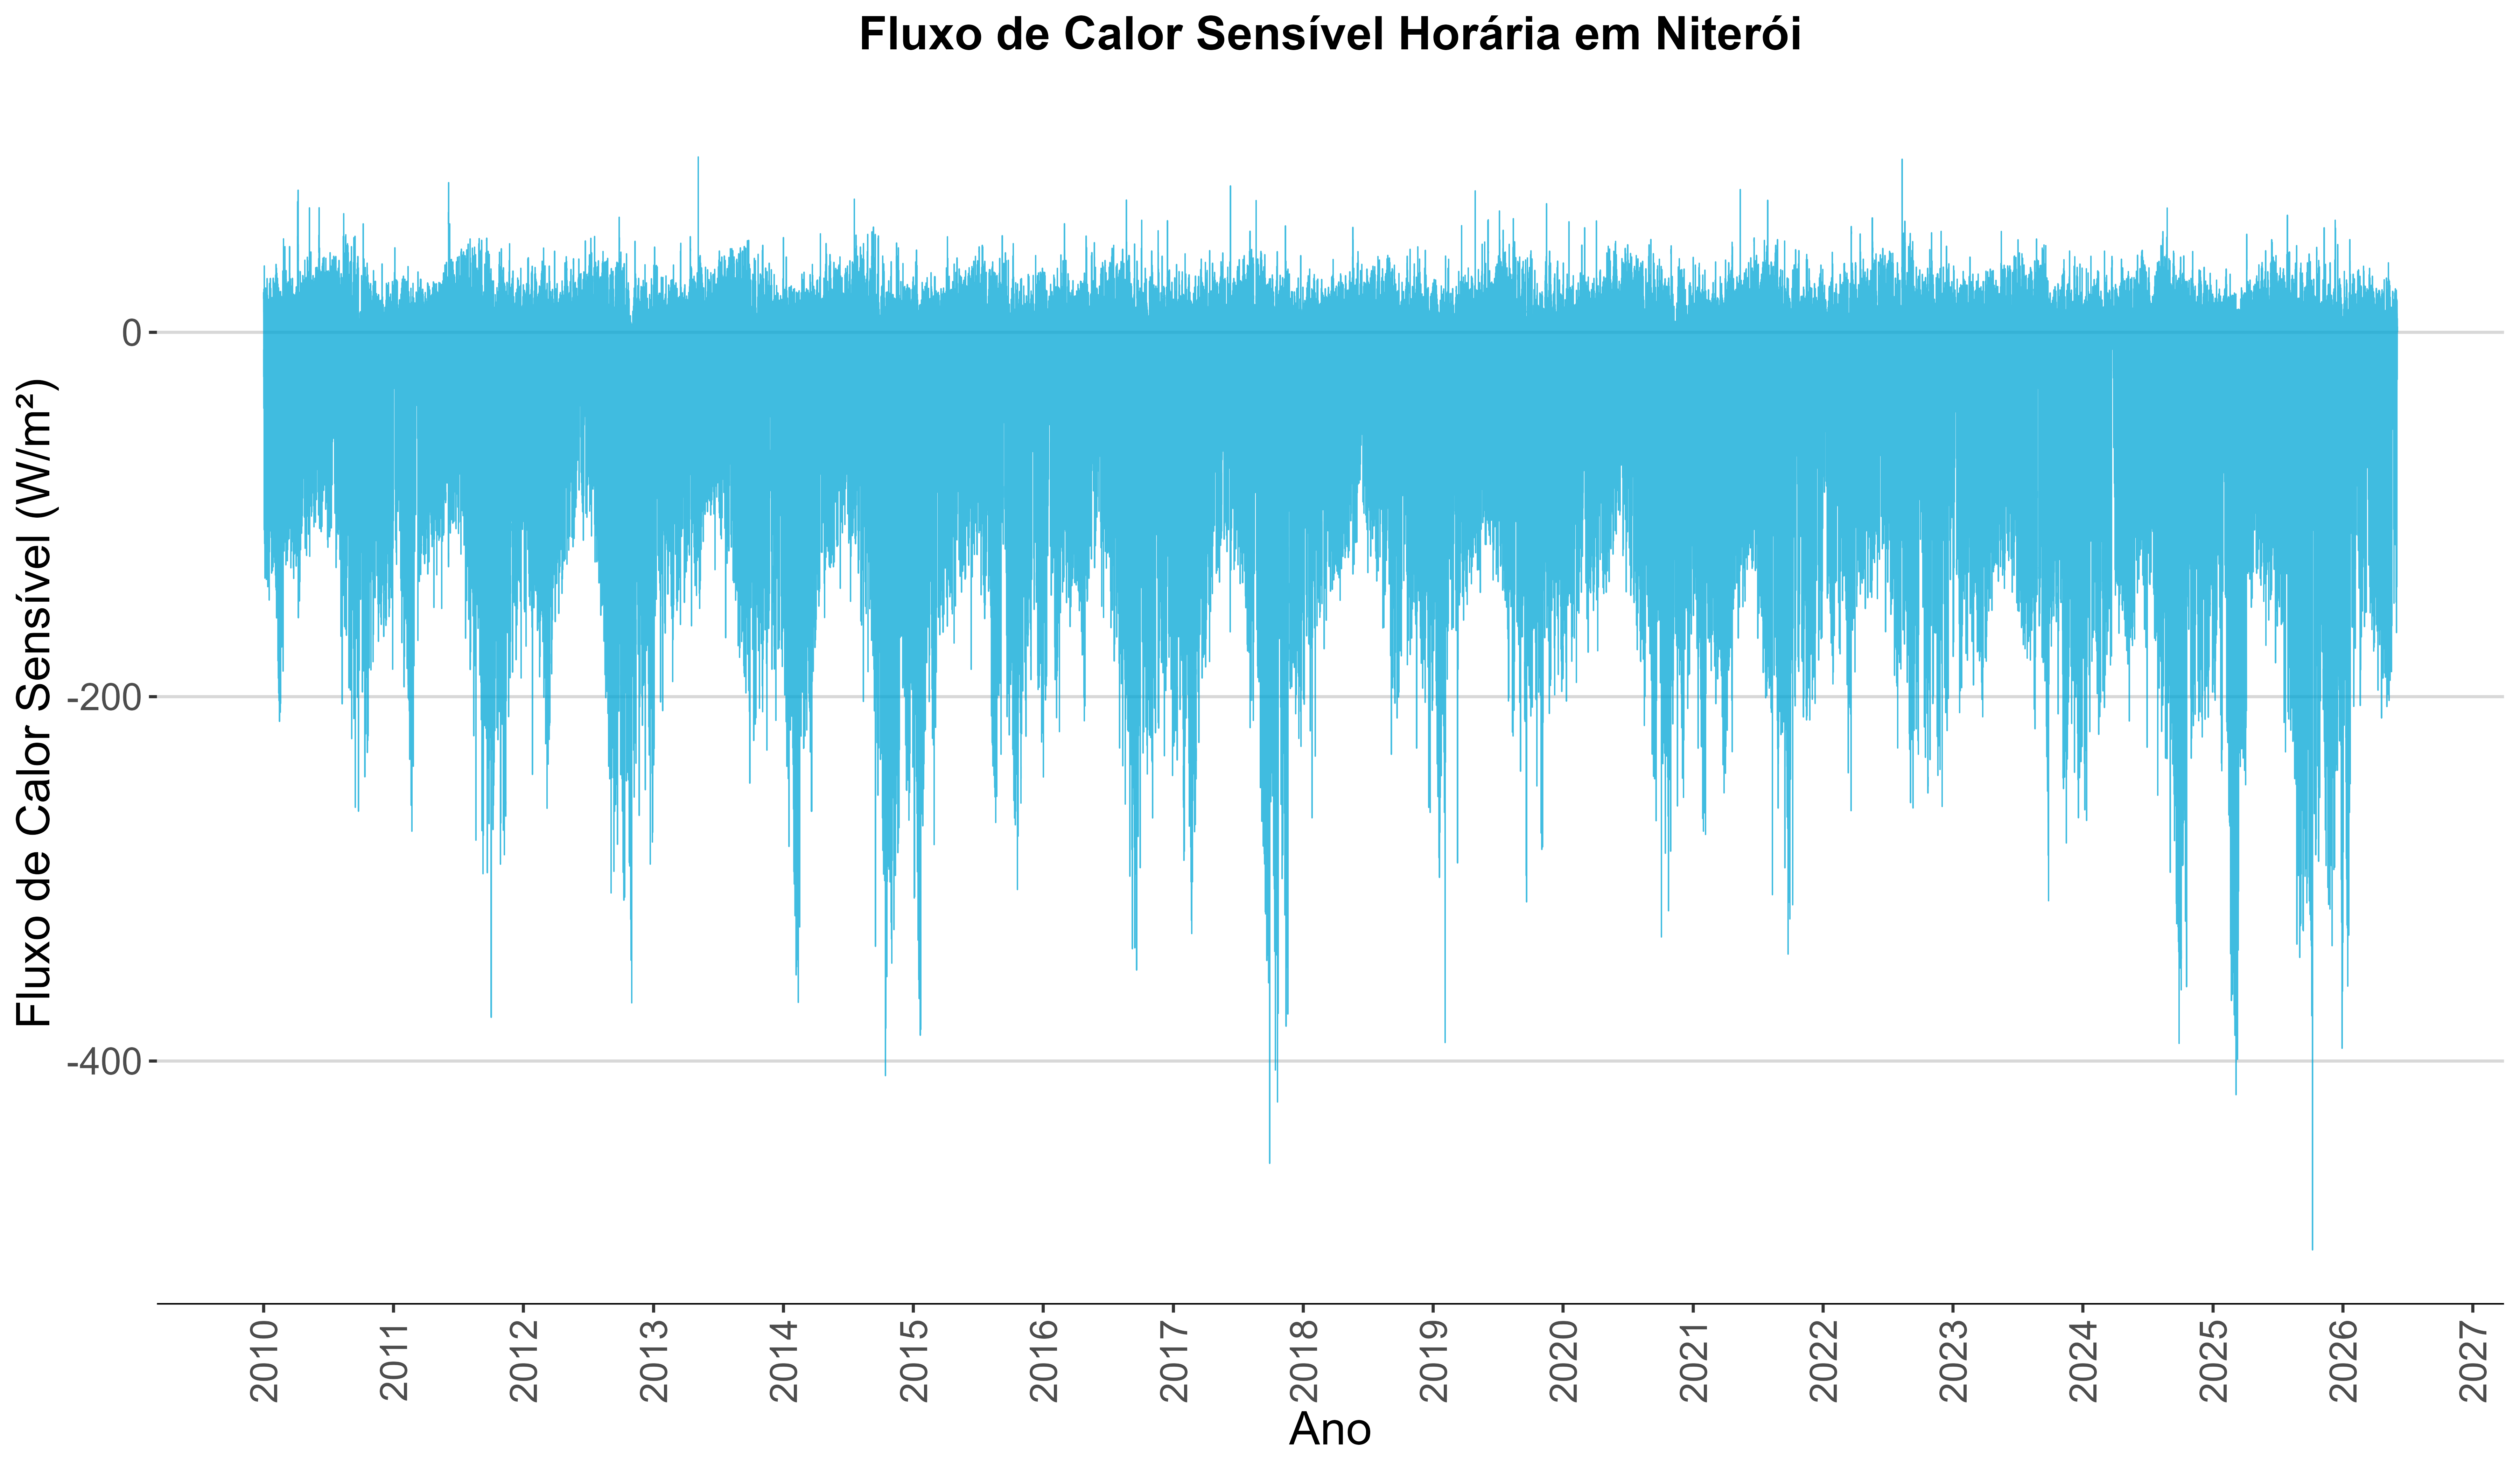
\includegraphics[keepaspectratio]{resultados/FluxoCalorSensivel/00_fluxocalorsensivel_horario.png}}

}

\caption{Fluxo de Calor Sensível Horário}

\end{figure}%

\begin{figure}[H]

{\centering \pandocbounded{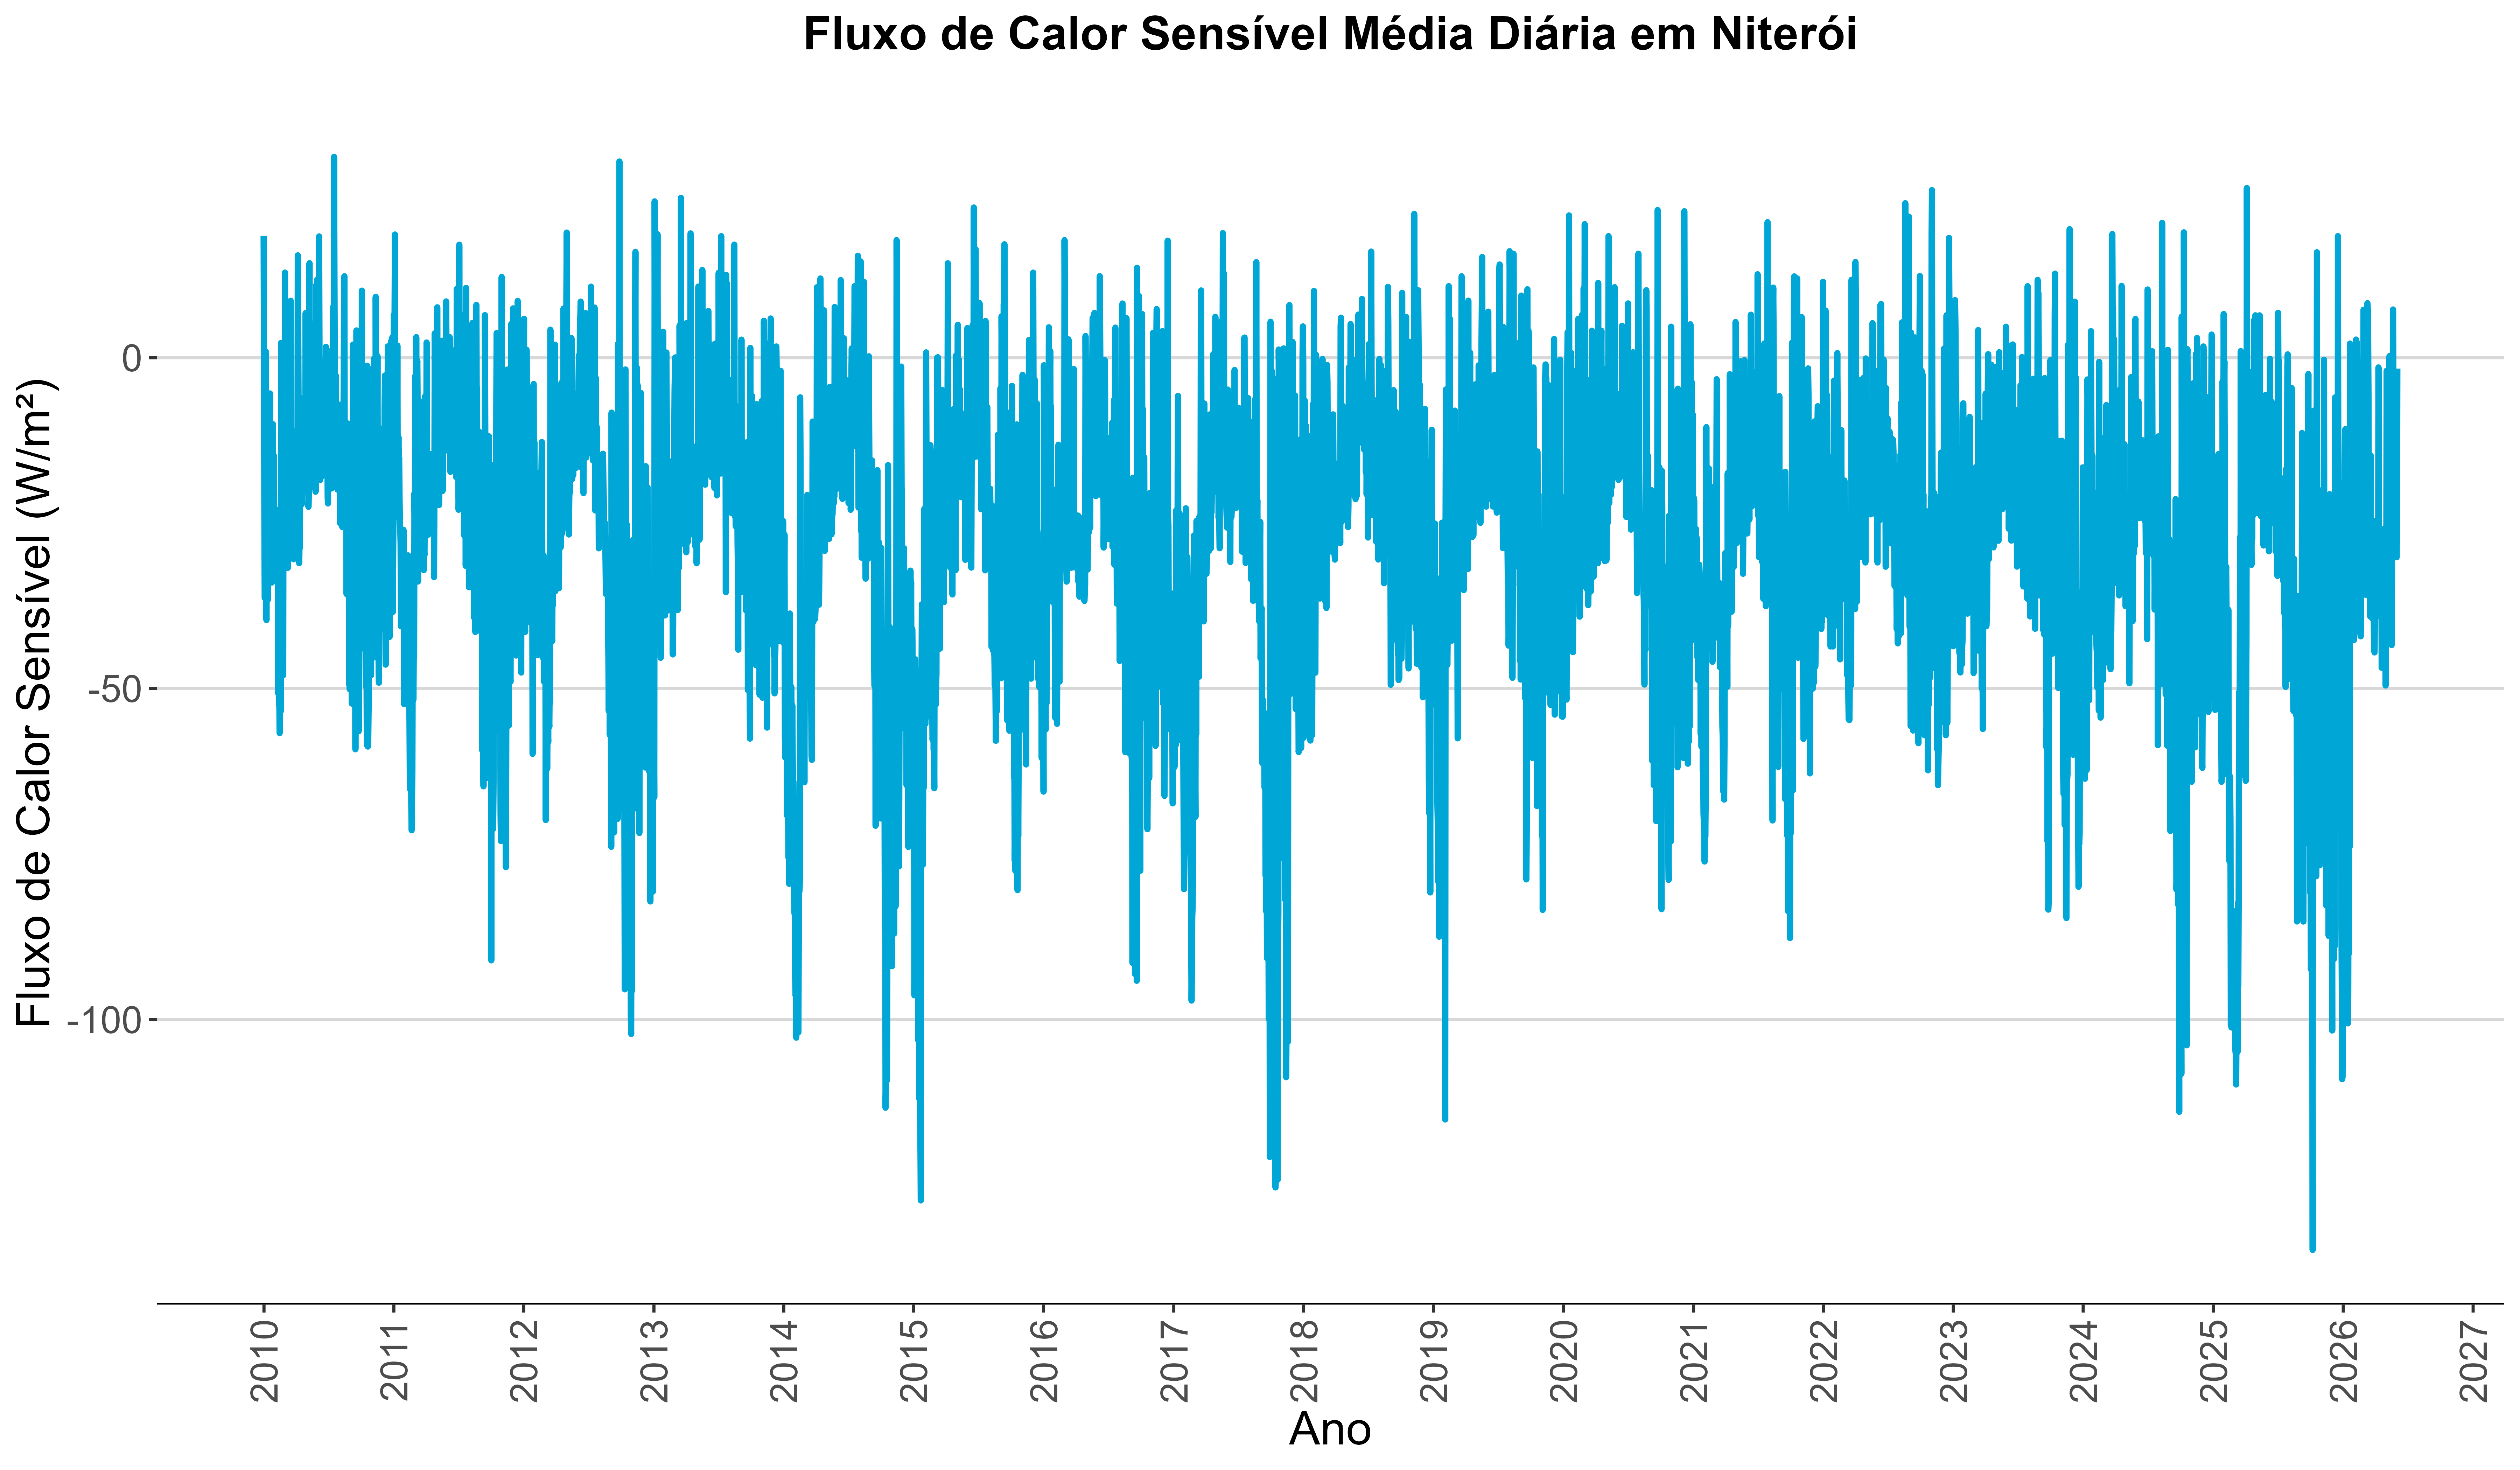
\includegraphics[keepaspectratio]{resultados/FluxoCalorSensivel/01_fluxocalorsensivel_diario.png}}

}

\caption{Fluxo de Calor Sensível Médio Diário}

\end{figure}%

\begin{figure}[H]

{\centering \pandocbounded{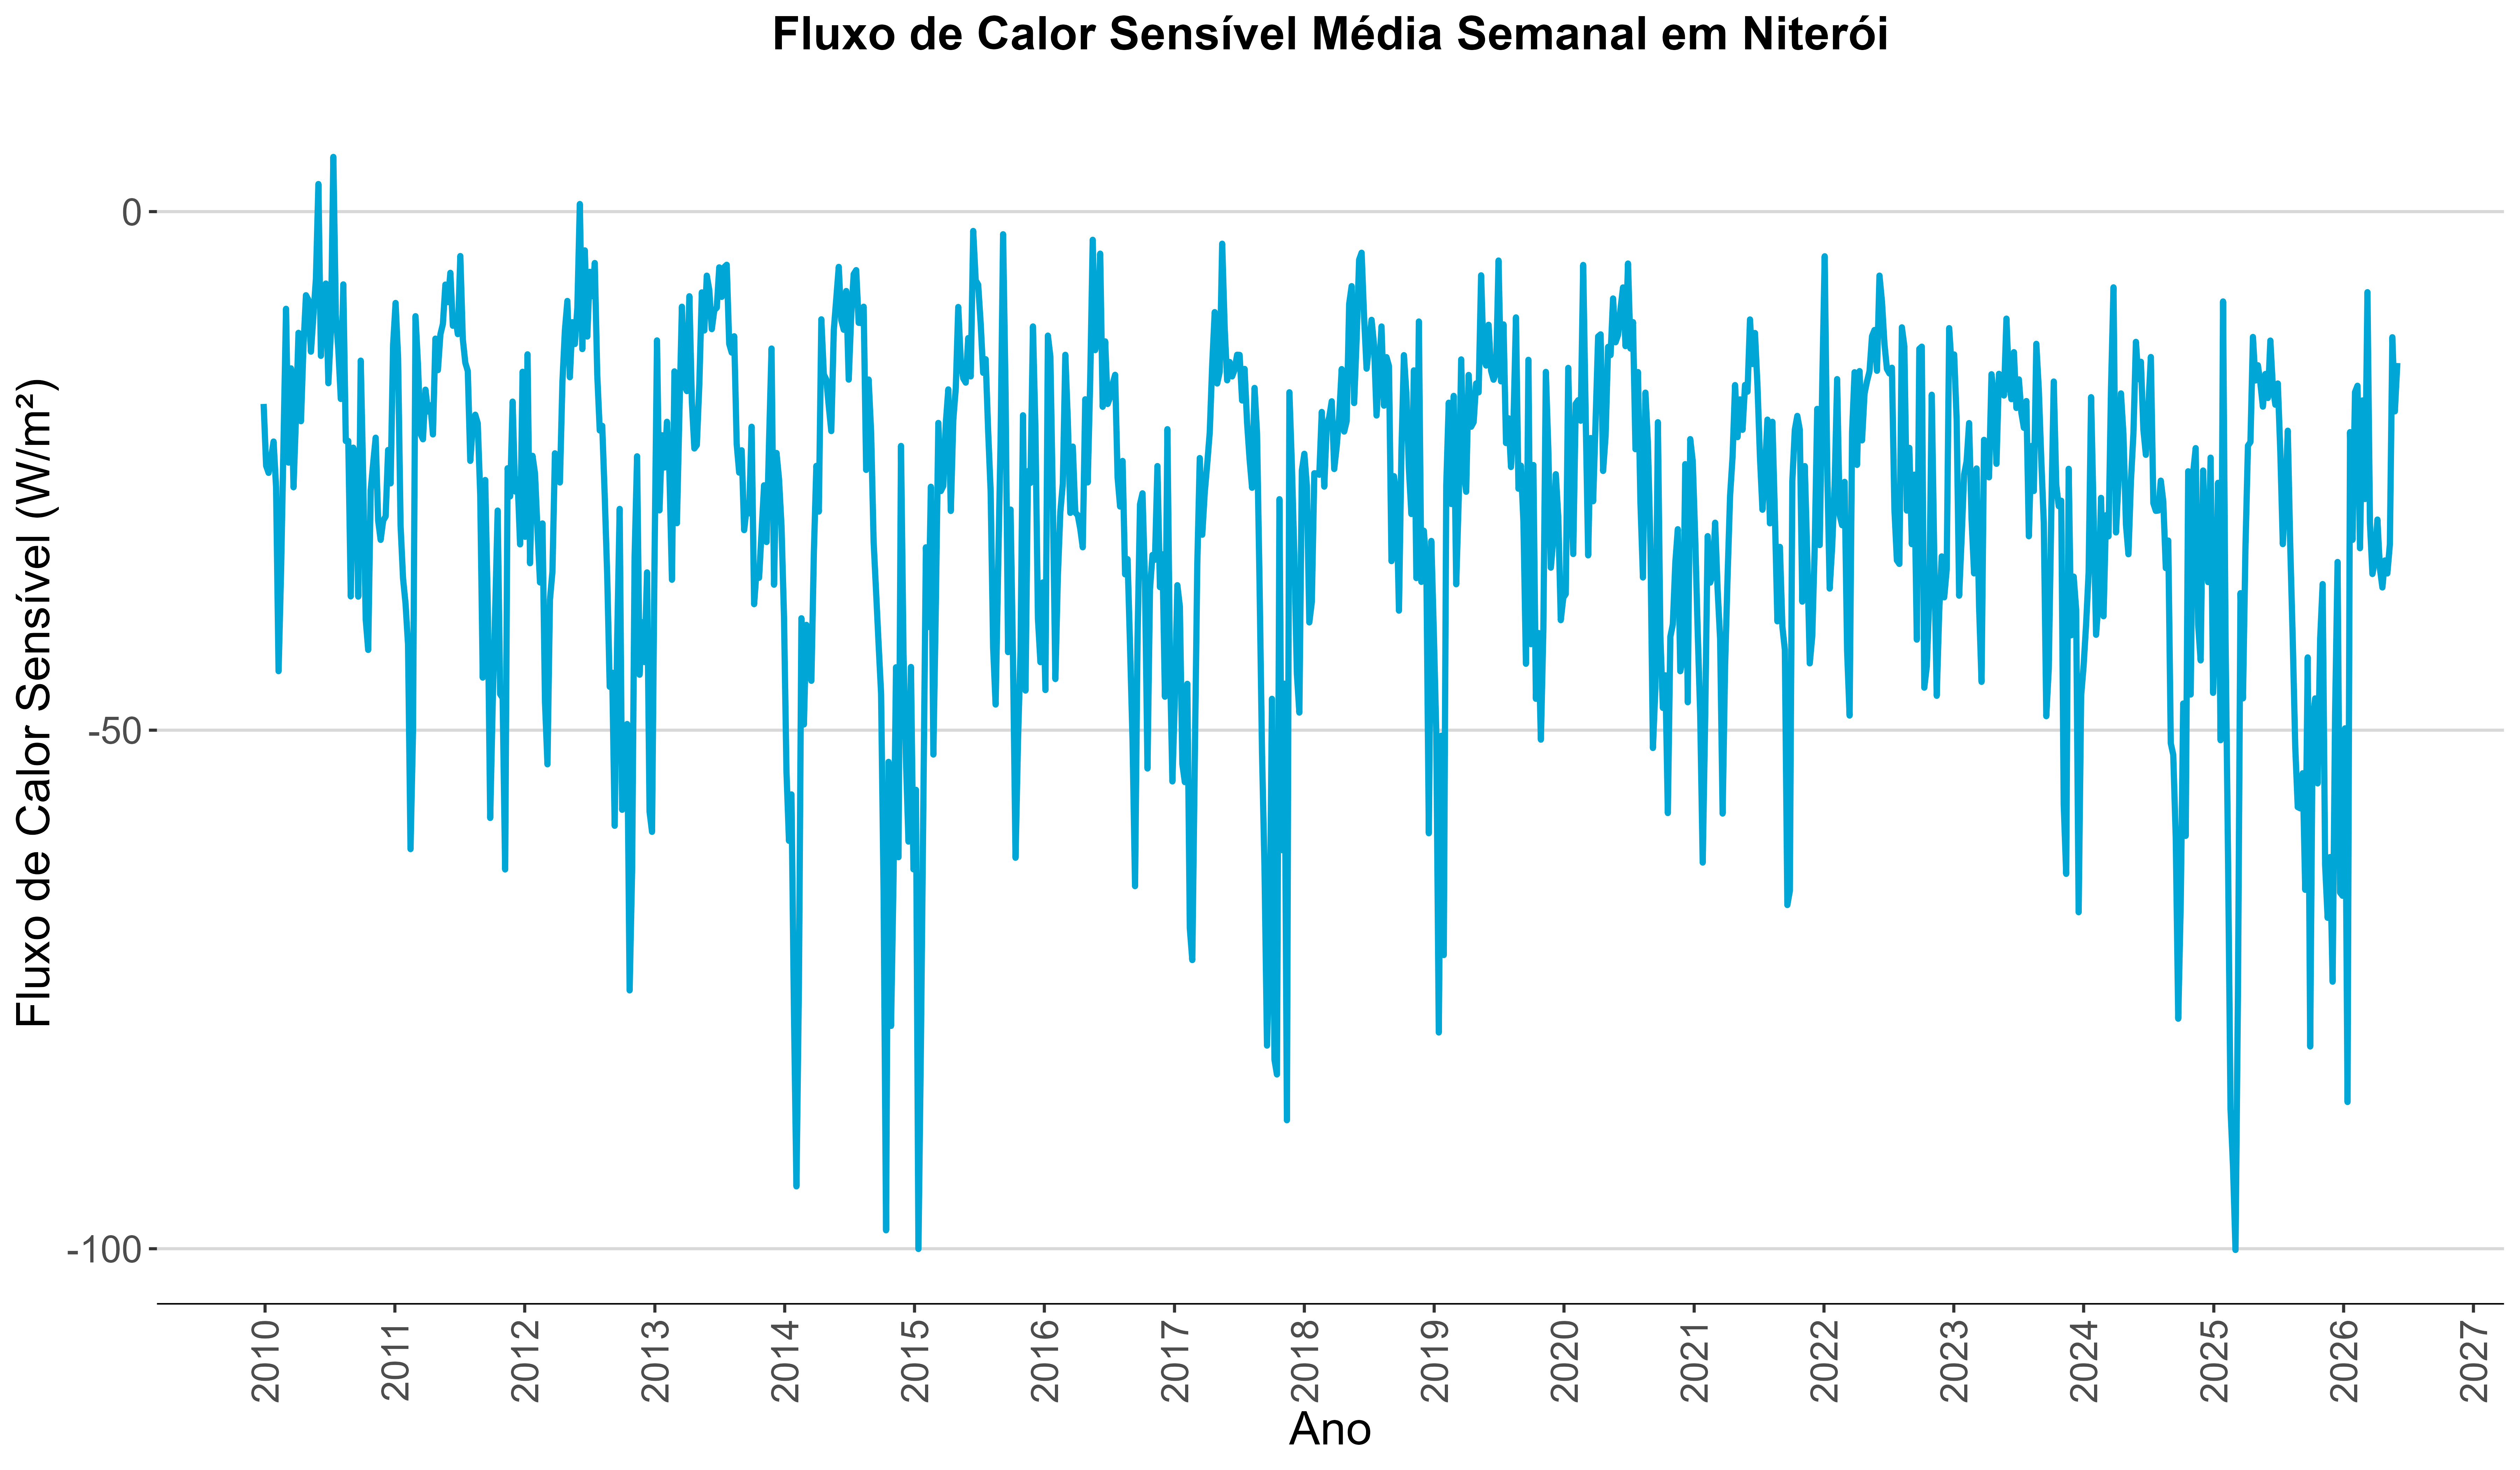
\includegraphics[keepaspectratio]{resultados/FluxoCalorSensivel/02_fluxocalorsensivel_semanal.png}}

}

\caption{Fluxo de Calor Sensível Médio Semanal}

\end{figure}%

\begin{figure}[H]

{\centering \pandocbounded{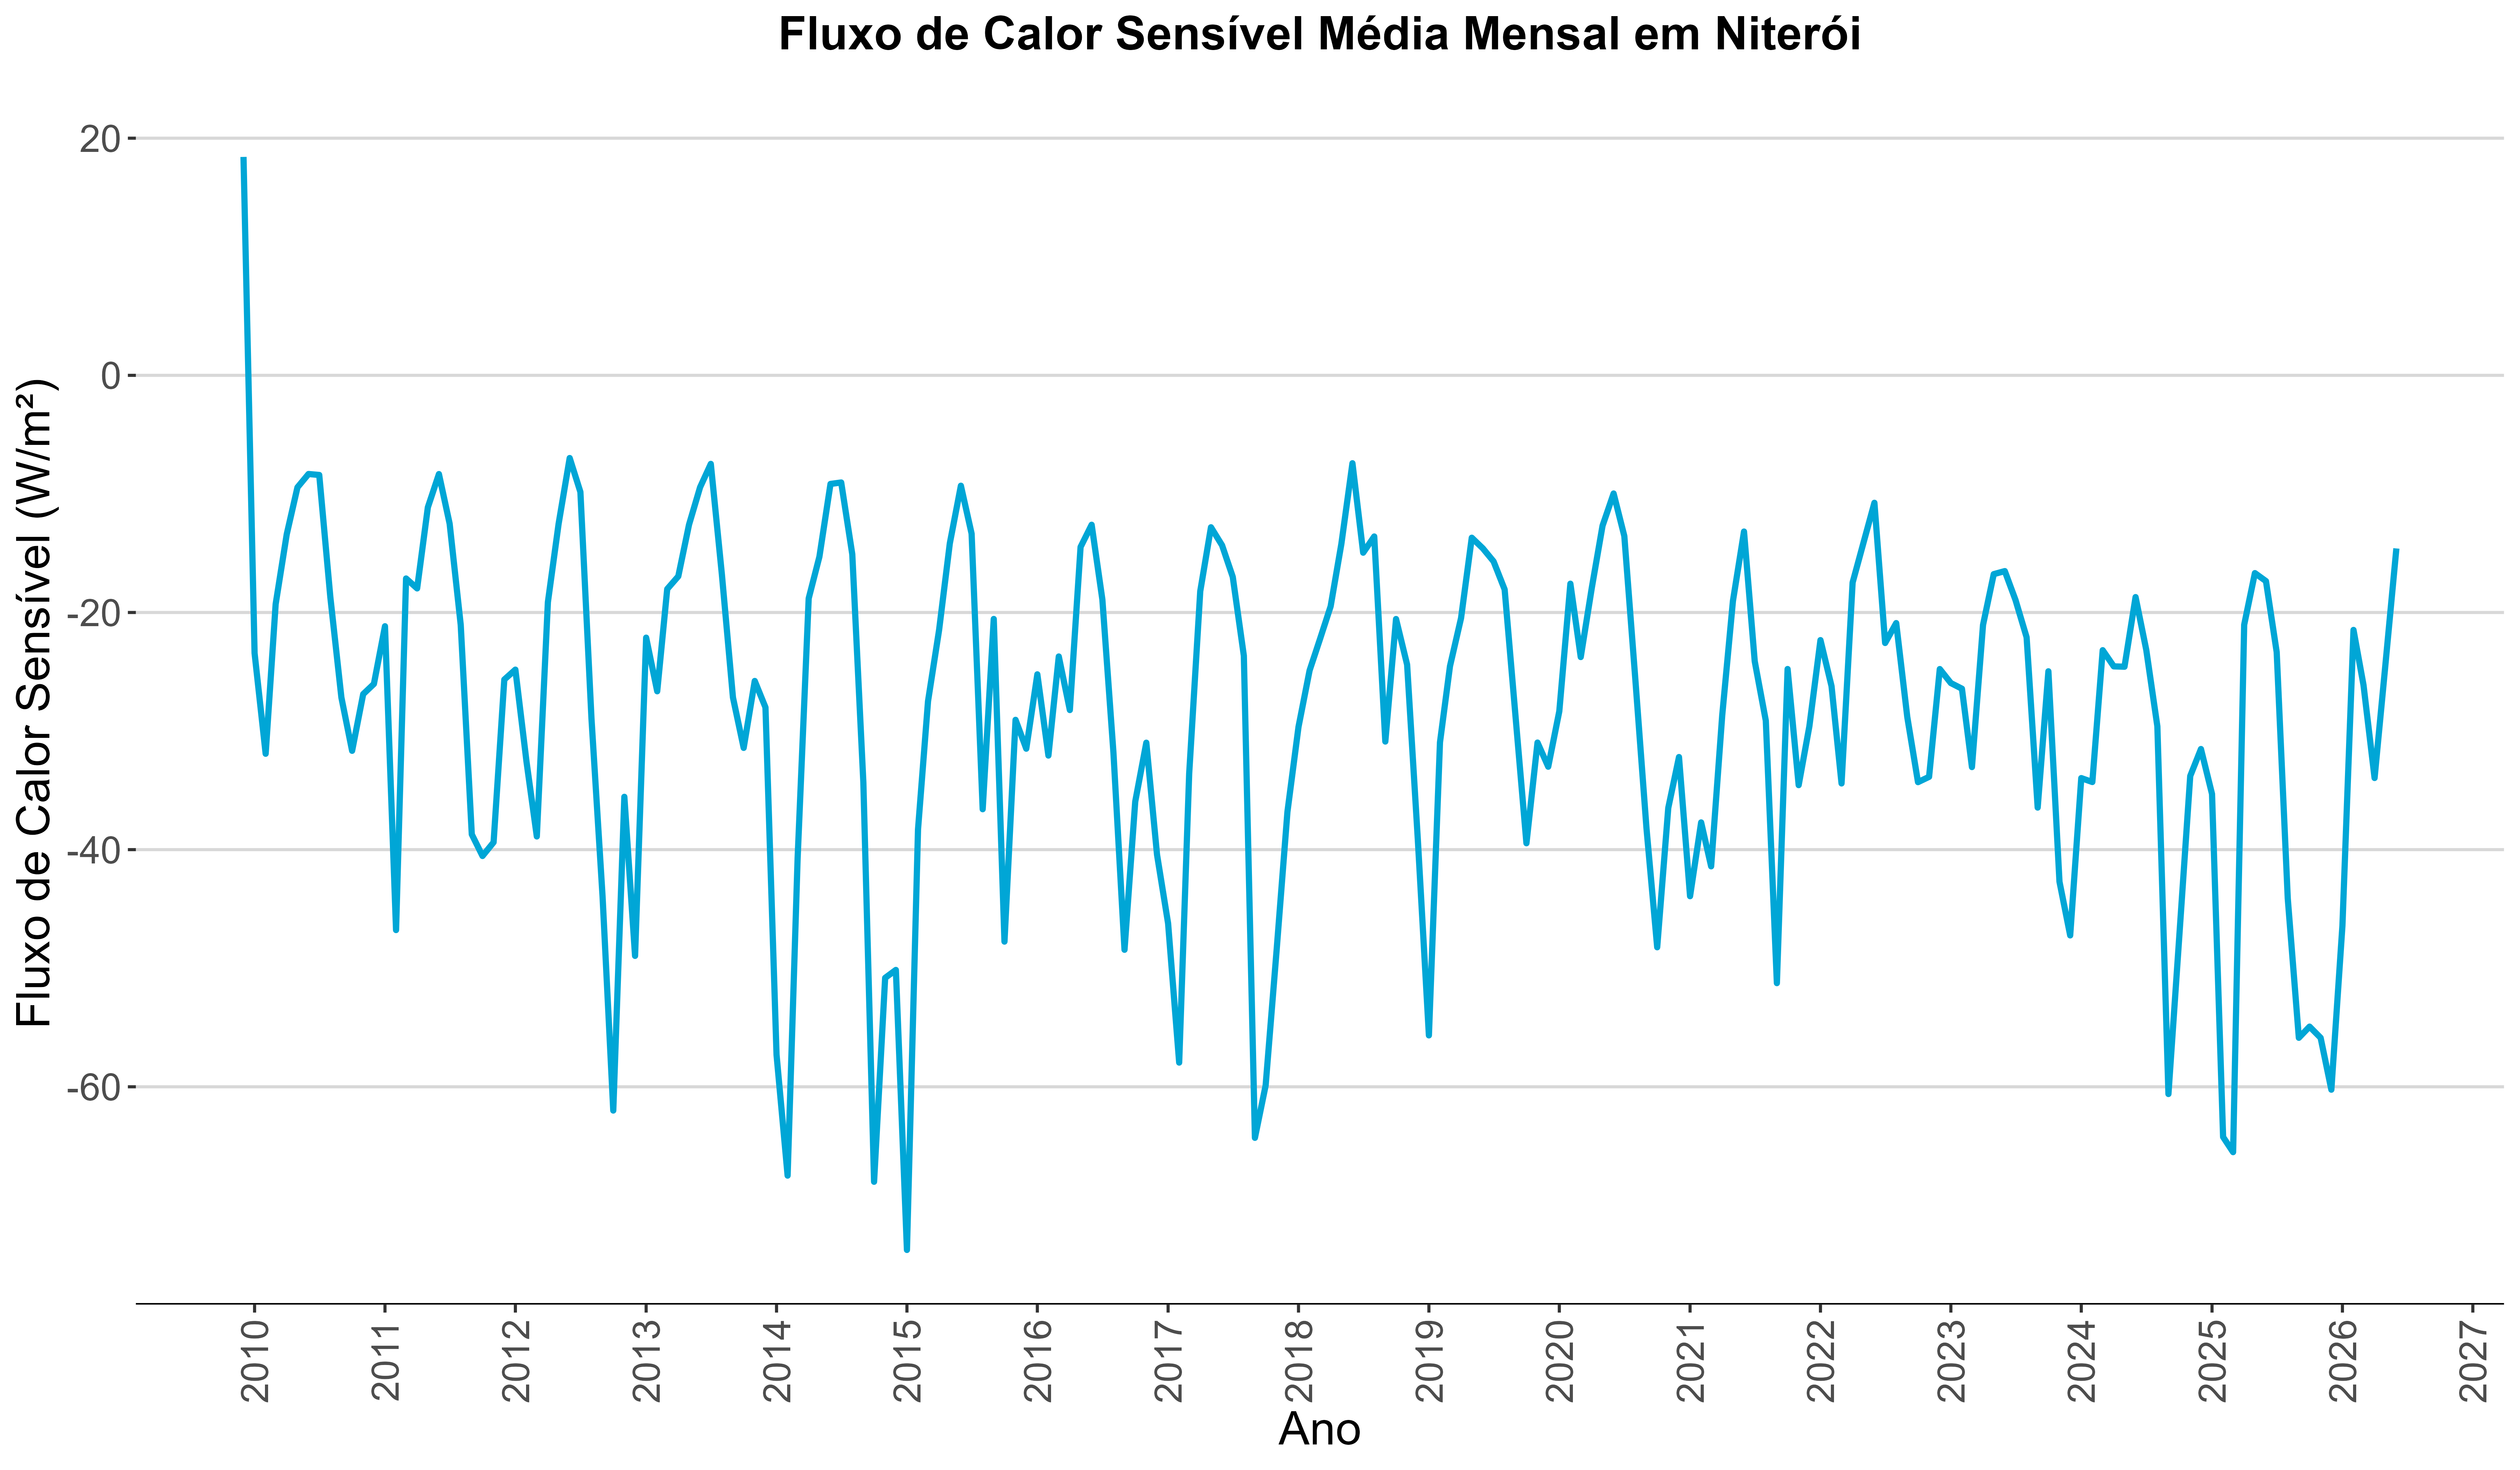
\includegraphics[keepaspectratio]{resultados/FluxoCalorSensivel/03_fluxocalorsensivel_mensal.png}}

}

\caption{Fluxo de Calor Sensível Médio Mensal}

\end{figure}%

\begin{figure}[H]

{\centering \pandocbounded{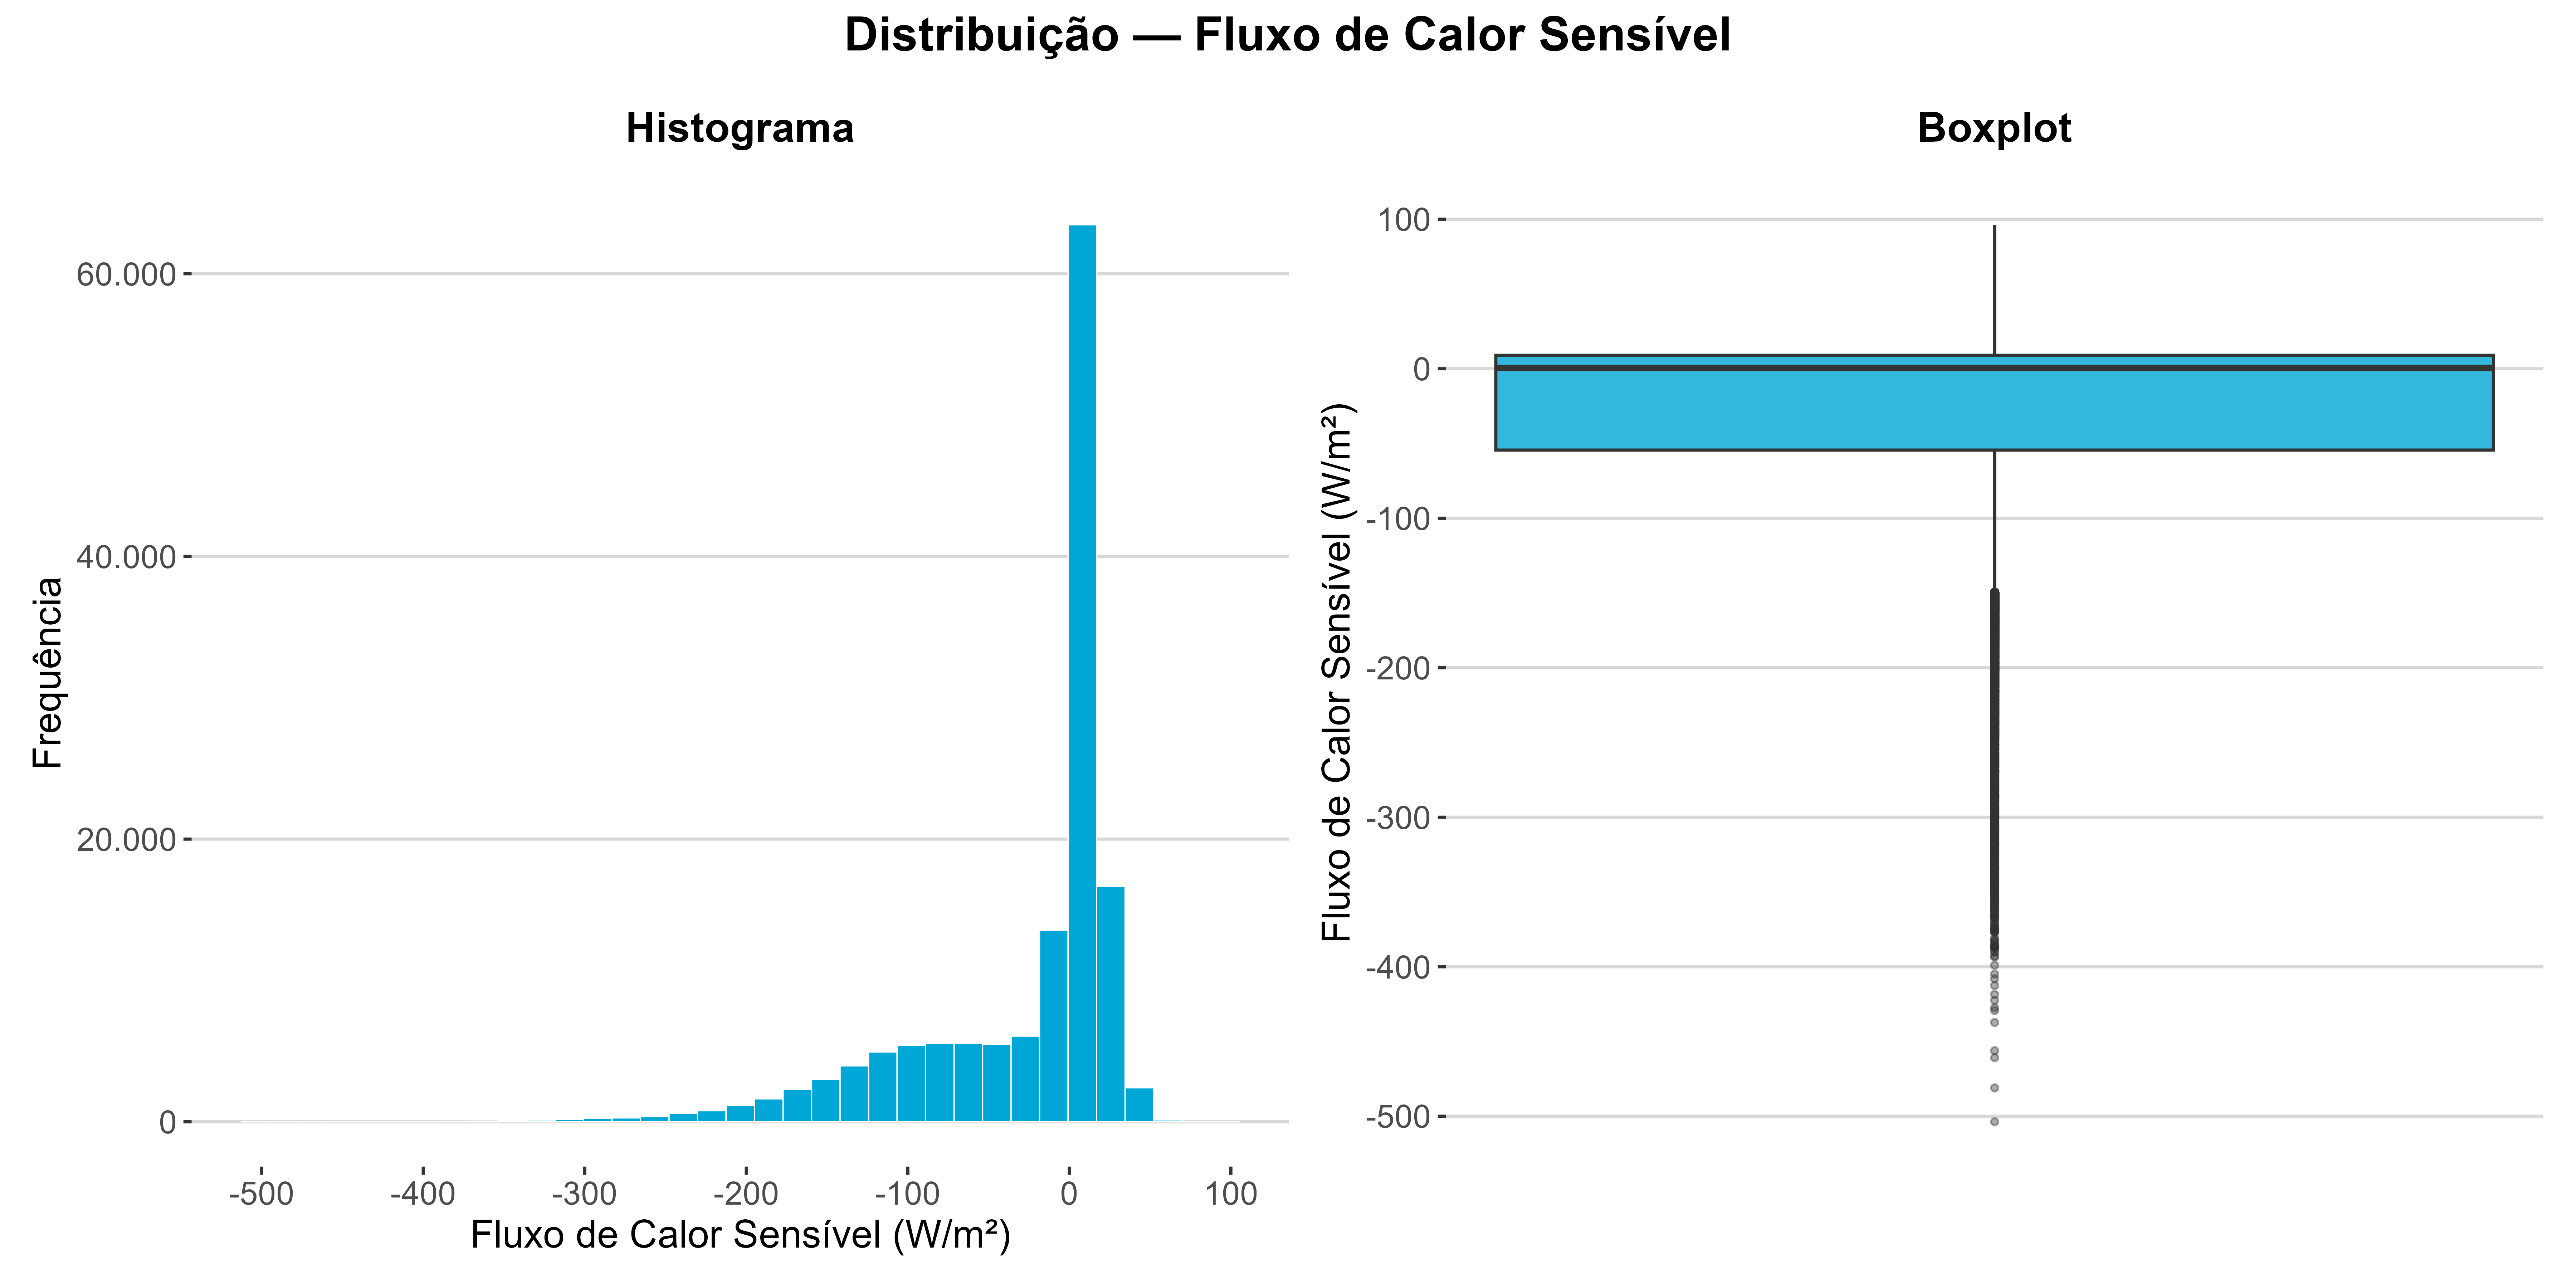
\includegraphics[keepaspectratio]{resultados/FluxoCalorSensivel/04_fluxocalorsensivel_distribuicao.png}}

}

\caption{Distribuição do Fluxo de Calor Sensível}

\end{figure}%

\paragraph{Principais Achados}\label{principais-achados-8}

O histograma revela distribuição assimétrica à esquerda, com moda
próxima a zero e cauda se estendendo até valores negativos elevados.

\subsubsection{Fluxo de Calor Latente}\label{fluxo-de-calor-latente}

\begin{figure}[H]

{\centering \pandocbounded{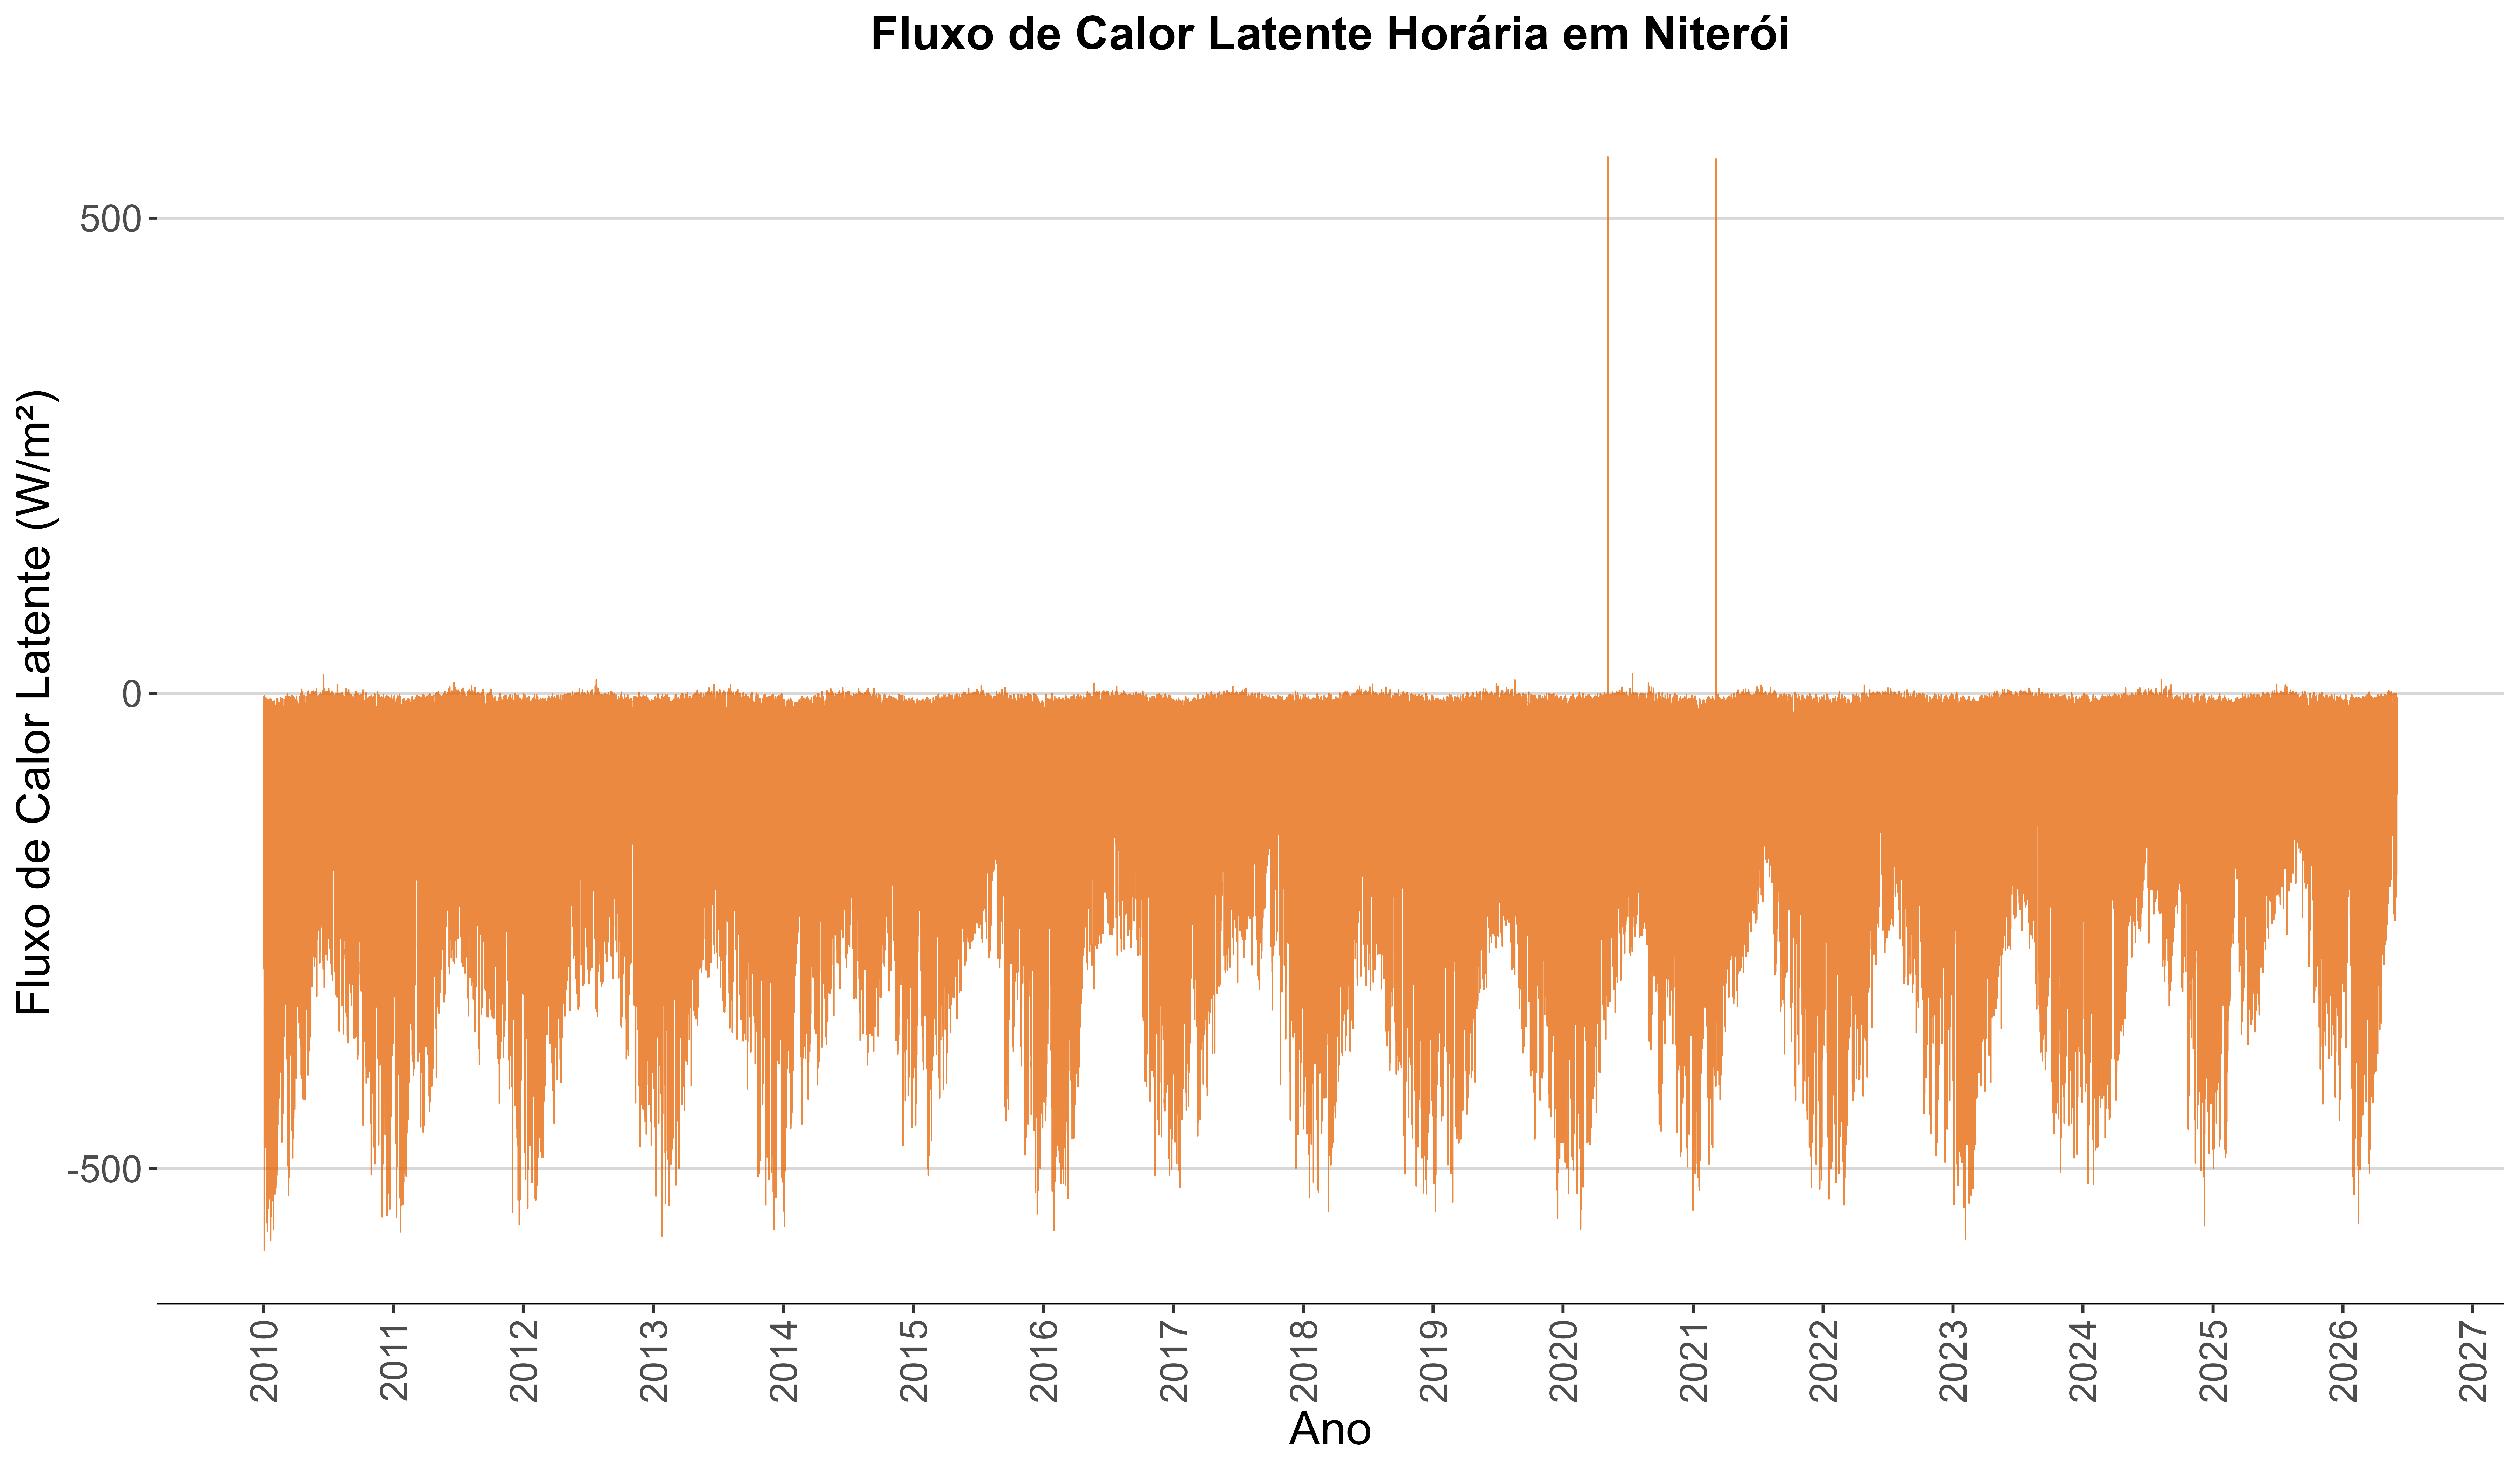
\includegraphics[keepaspectratio]{resultados/FluxoCalorLatente/00_fluxocalorlatente_horario.png}}

}

\caption{Fluxo de Calor Latente Horário}

\end{figure}%

\begin{figure}[H]

{\centering \pandocbounded{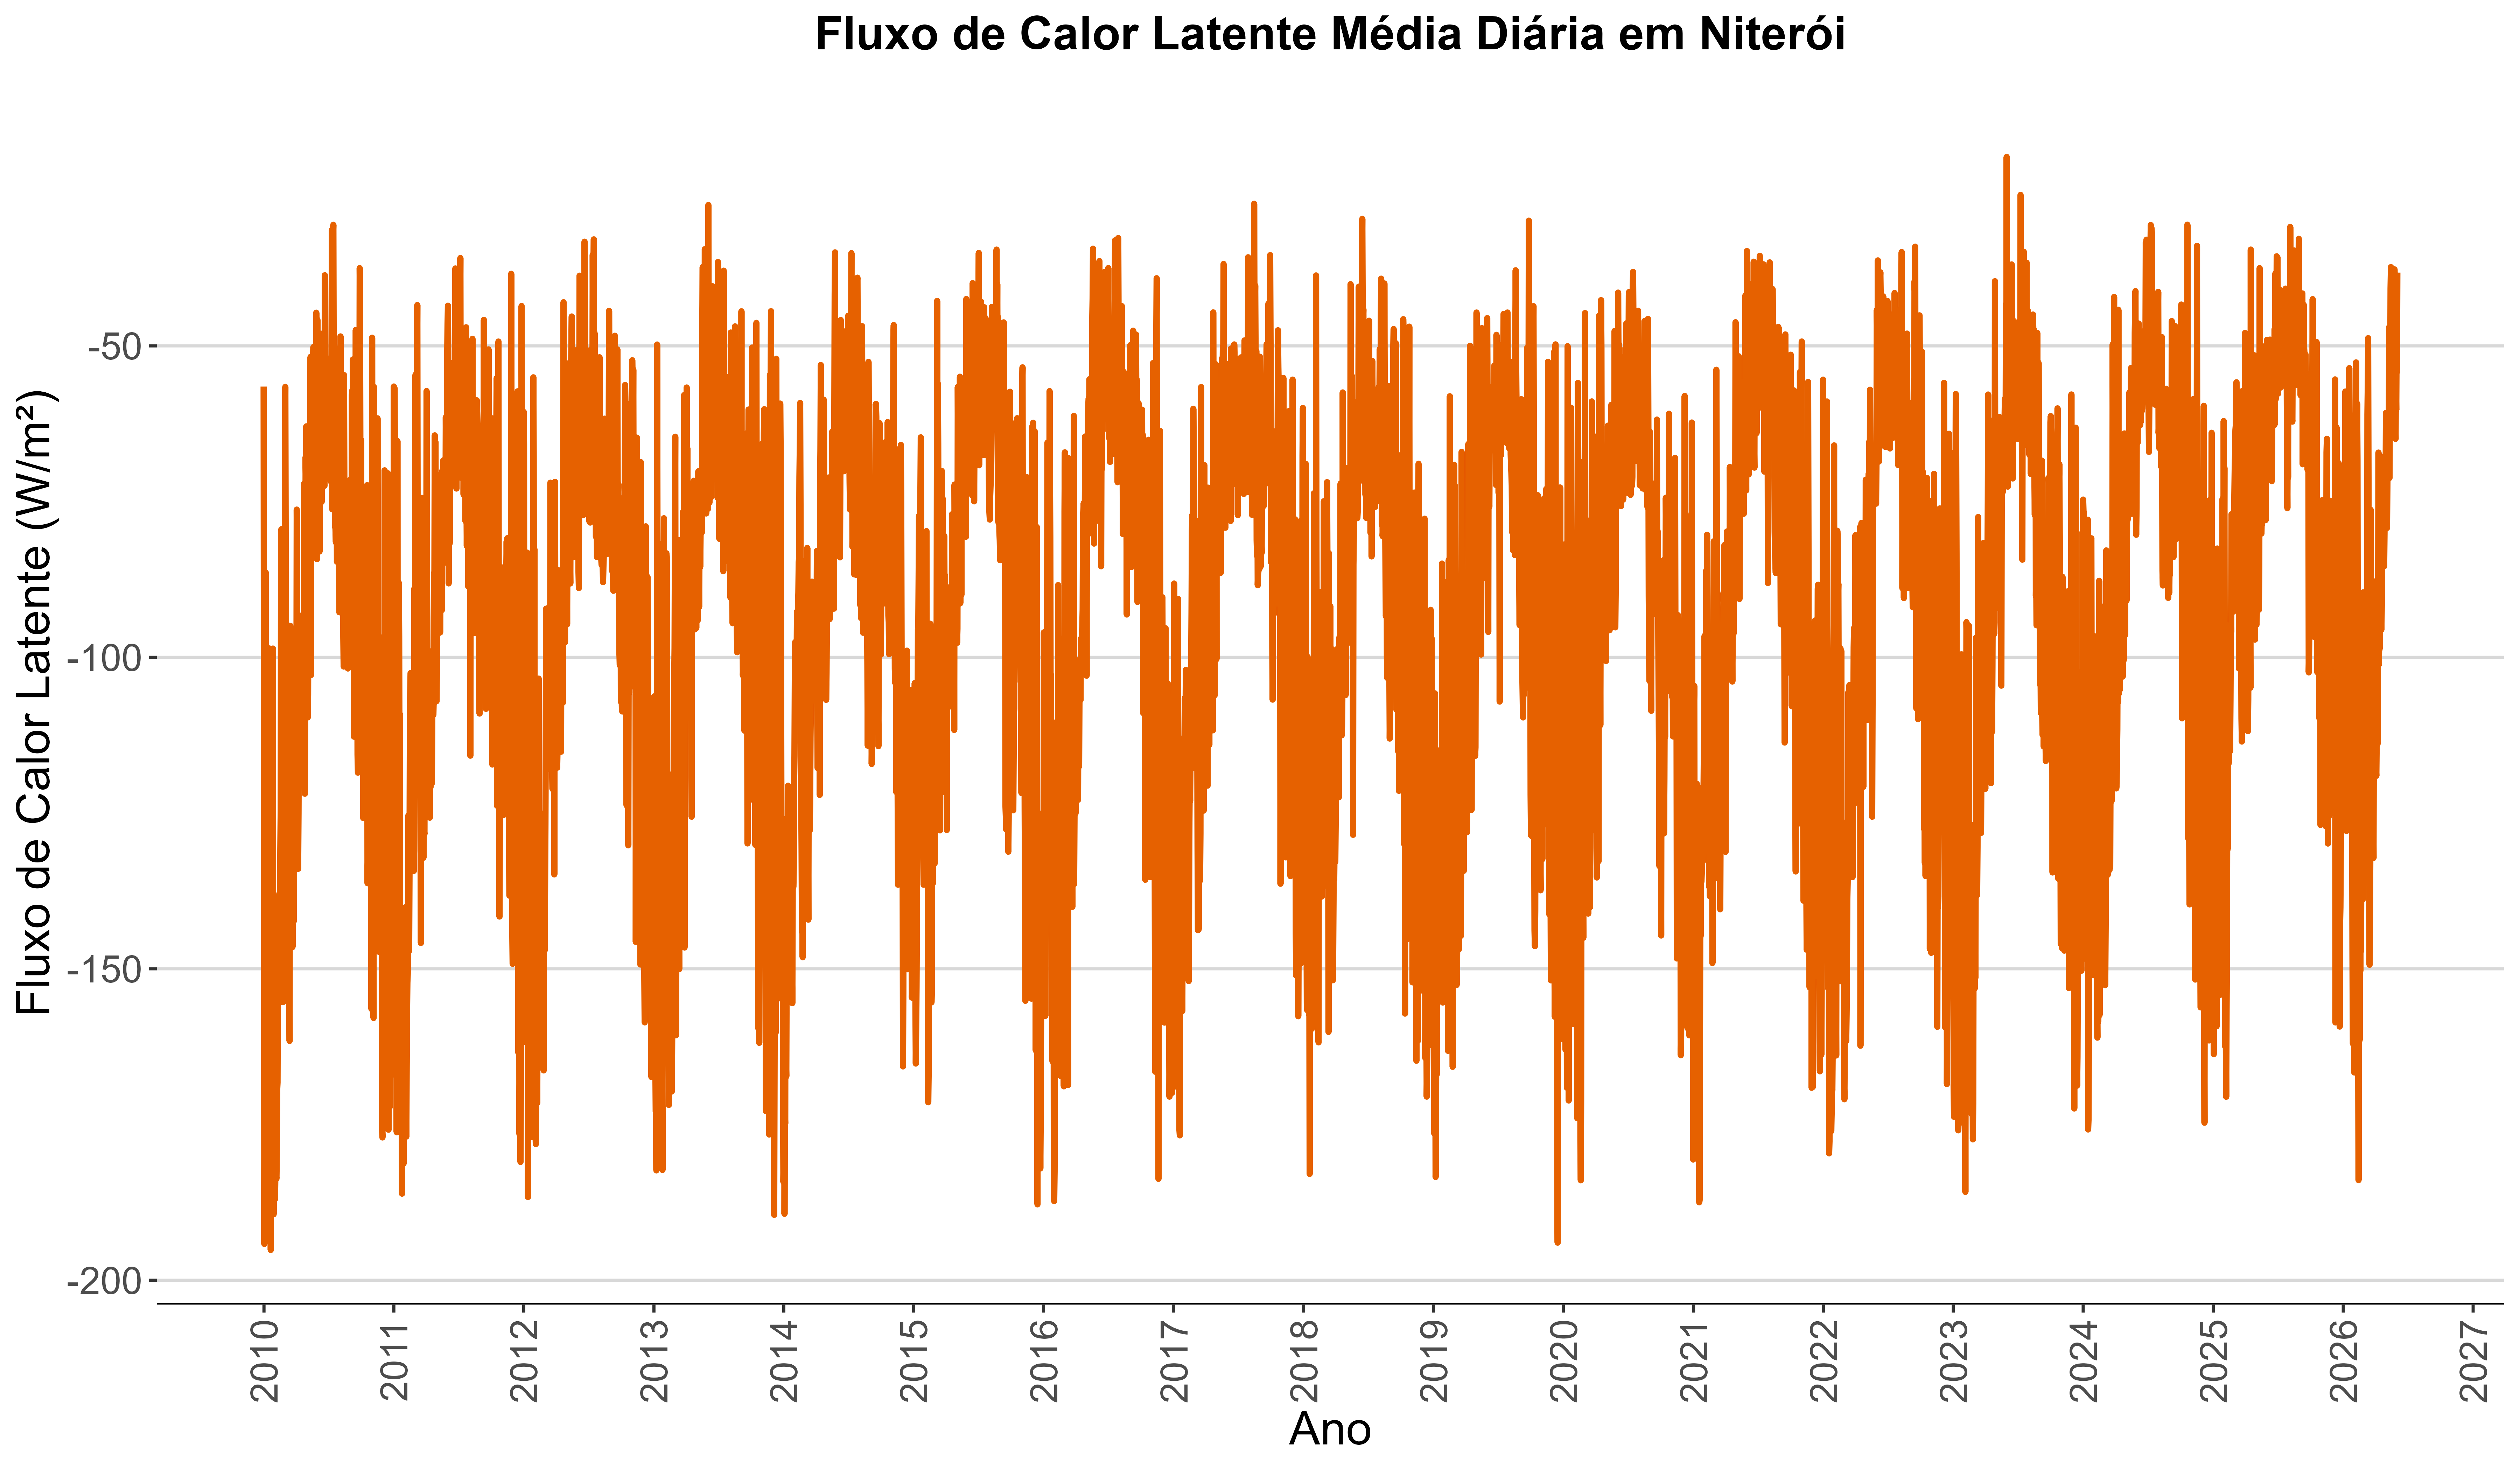
\includegraphics[keepaspectratio]{resultados/FluxoCalorLatente/01_fluxocalorlatente_diario.png}}

}

\caption{Fluxo de Calor Latente Médio Diário}

\end{figure}%

\begin{figure}[H]

{\centering \pandocbounded{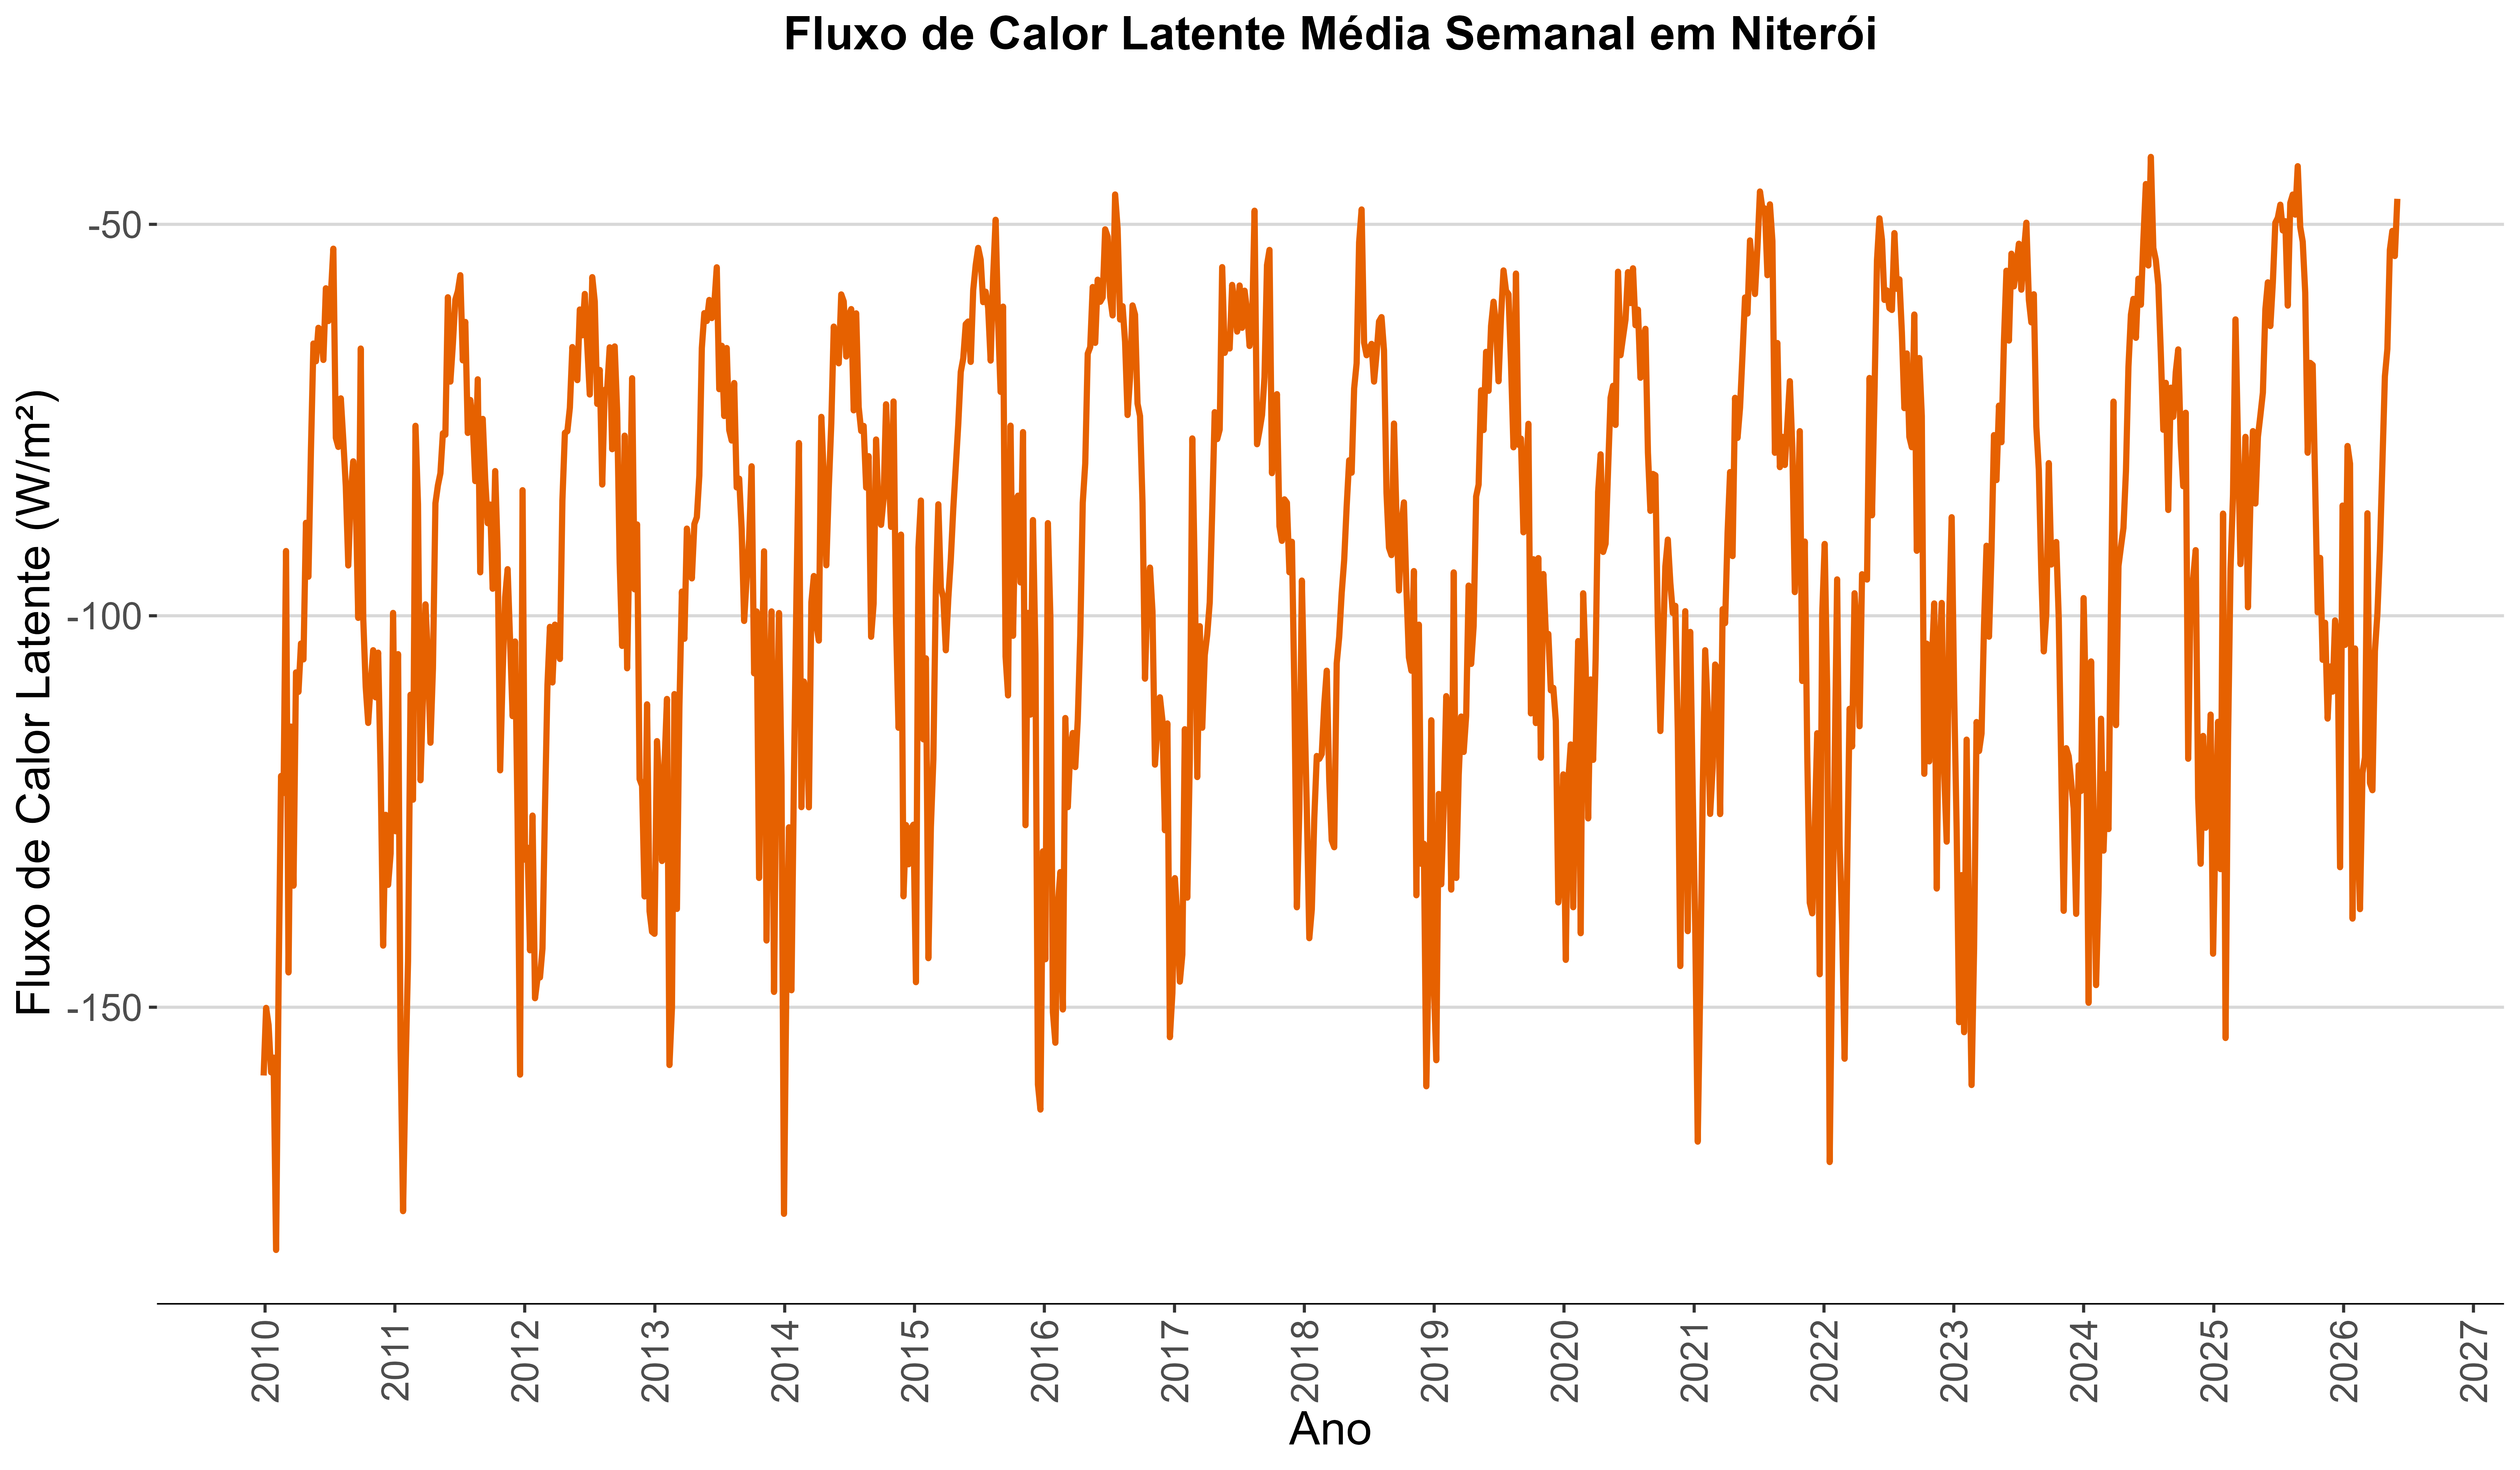
\includegraphics[keepaspectratio]{resultados/FluxoCalorLatente/02_fluxocalorlatente_semanal.png}}

}

\caption{Fluxo de Calor Latente Médio Semanal}

\end{figure}%

\begin{figure}[H]

{\centering \pandocbounded{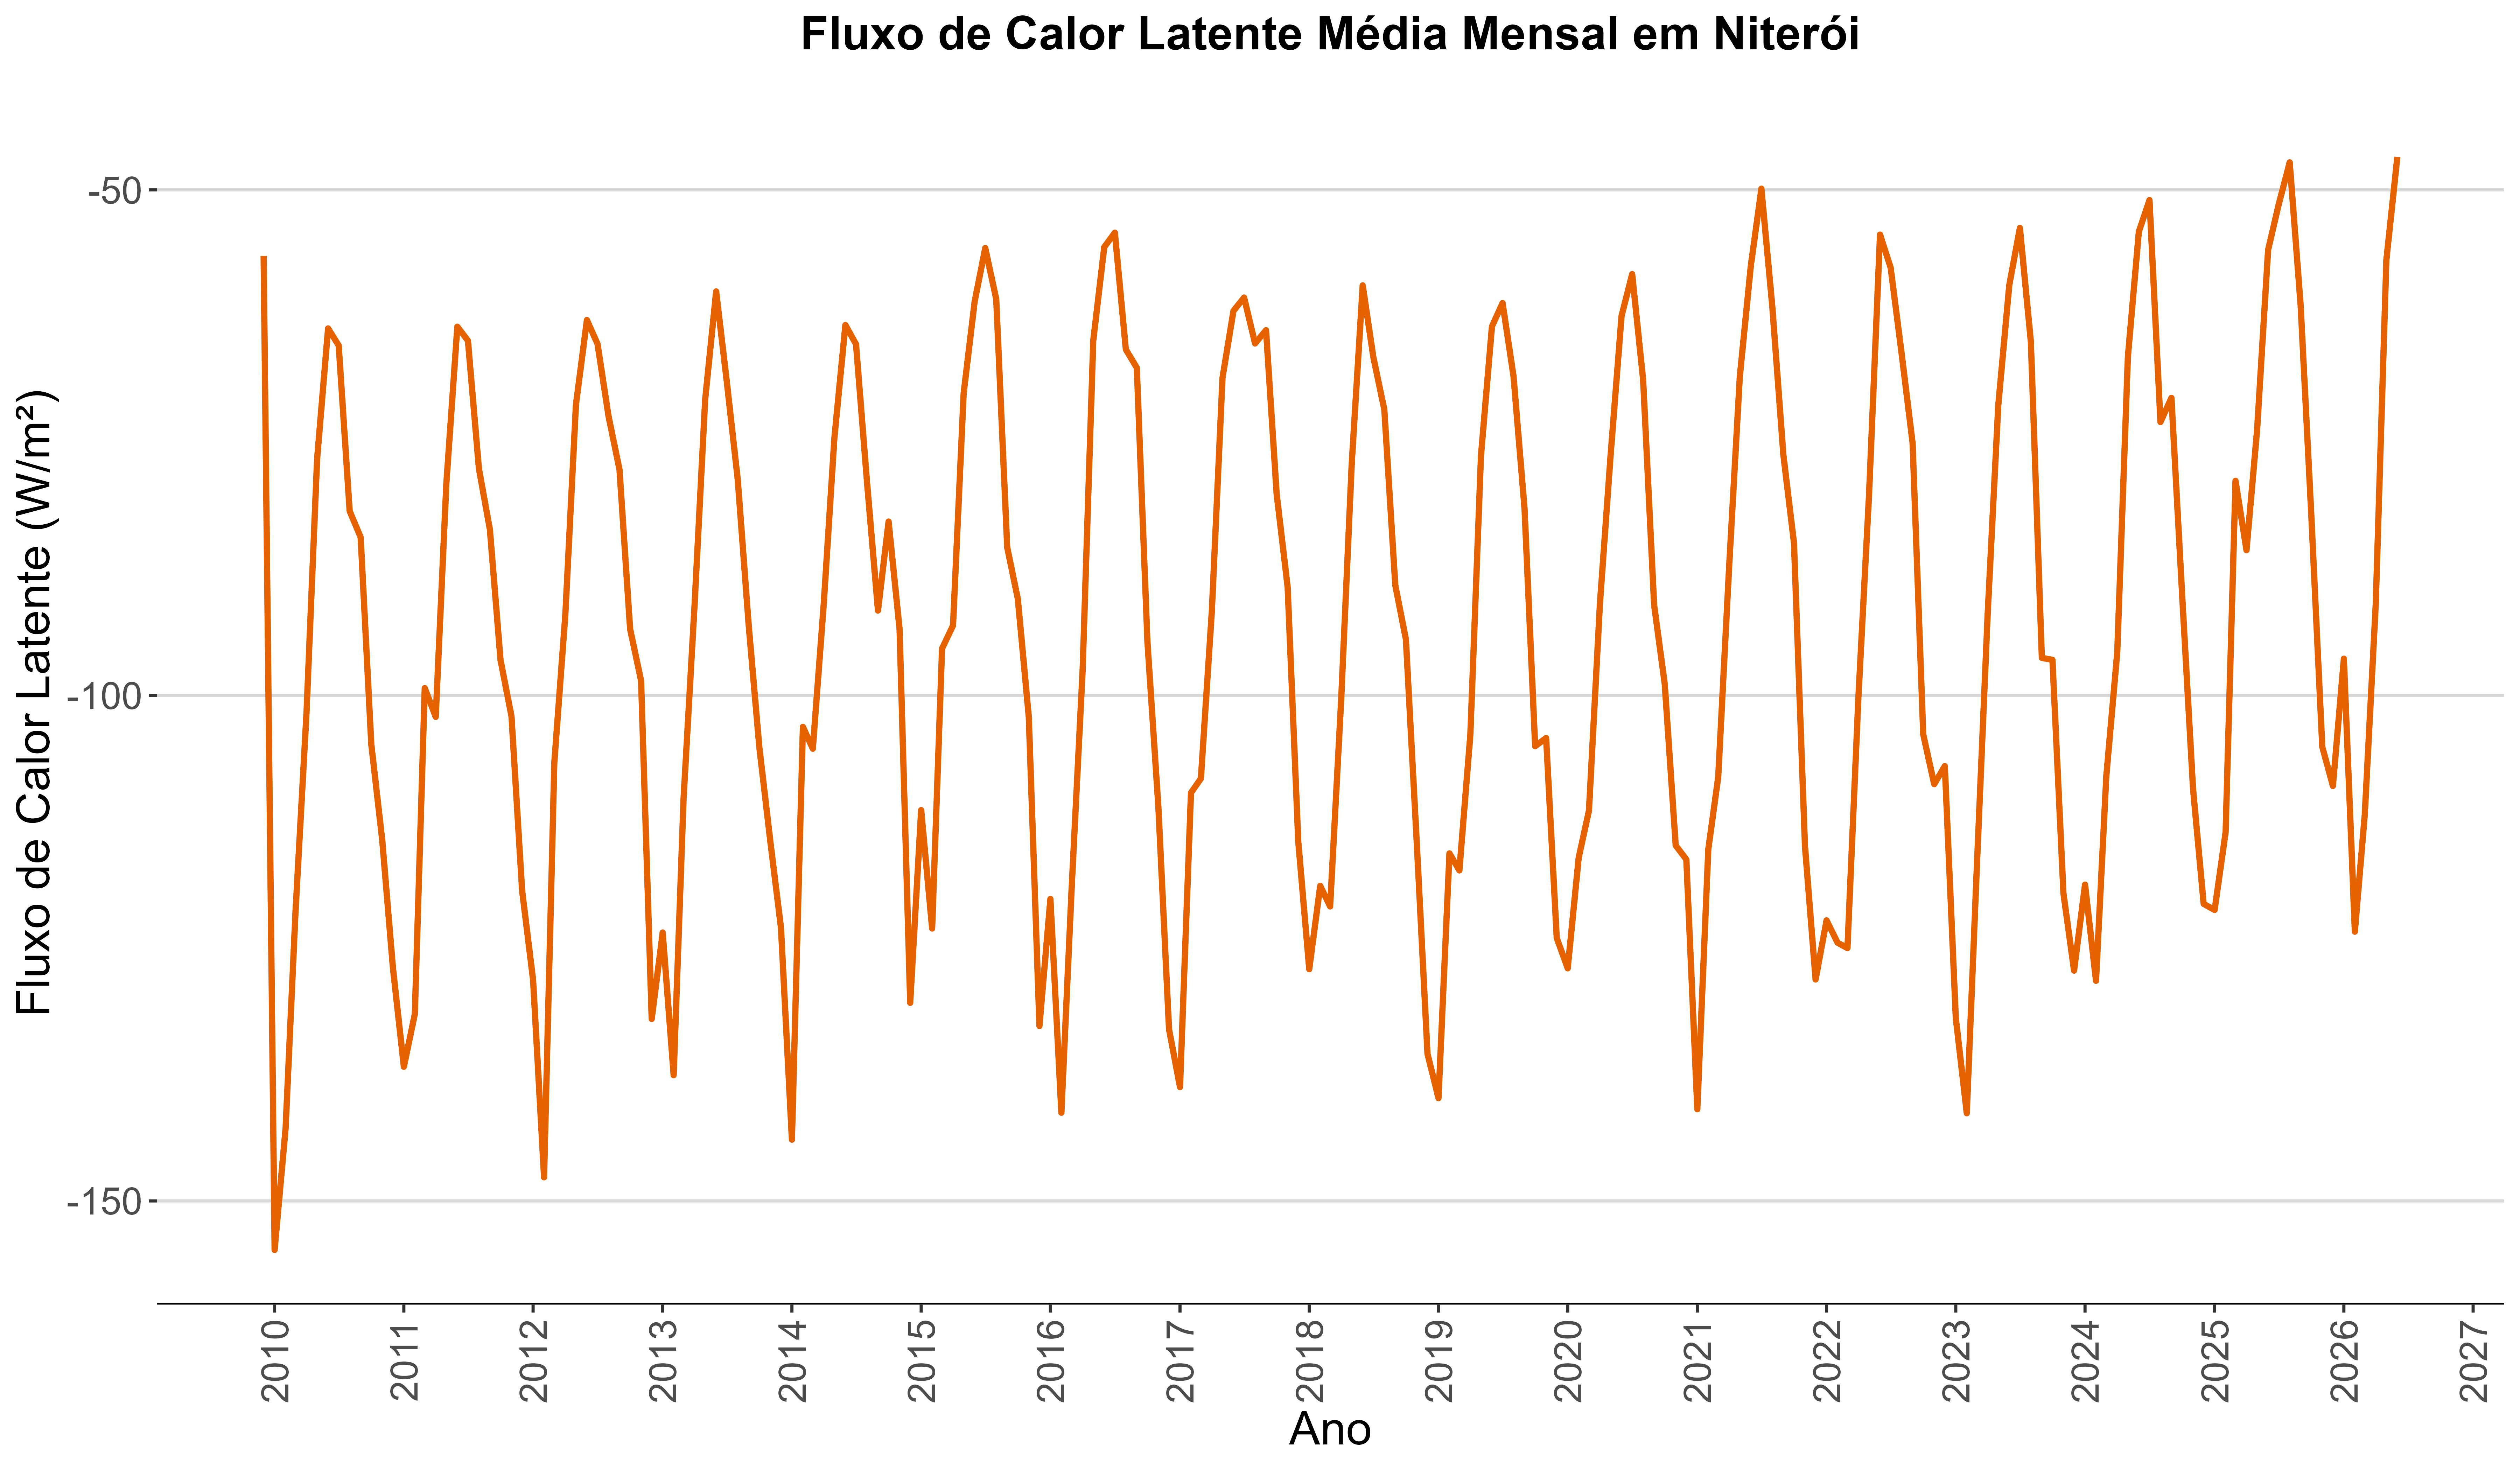
\includegraphics[keepaspectratio]{resultados/FluxoCalorLatente/03_fluxocalorlatente_mensal.png}}

}

\caption{Fluxo de Calor Latente Médio Mensal}

\end{figure}%

\begin{figure}[H]

{\centering \pandocbounded{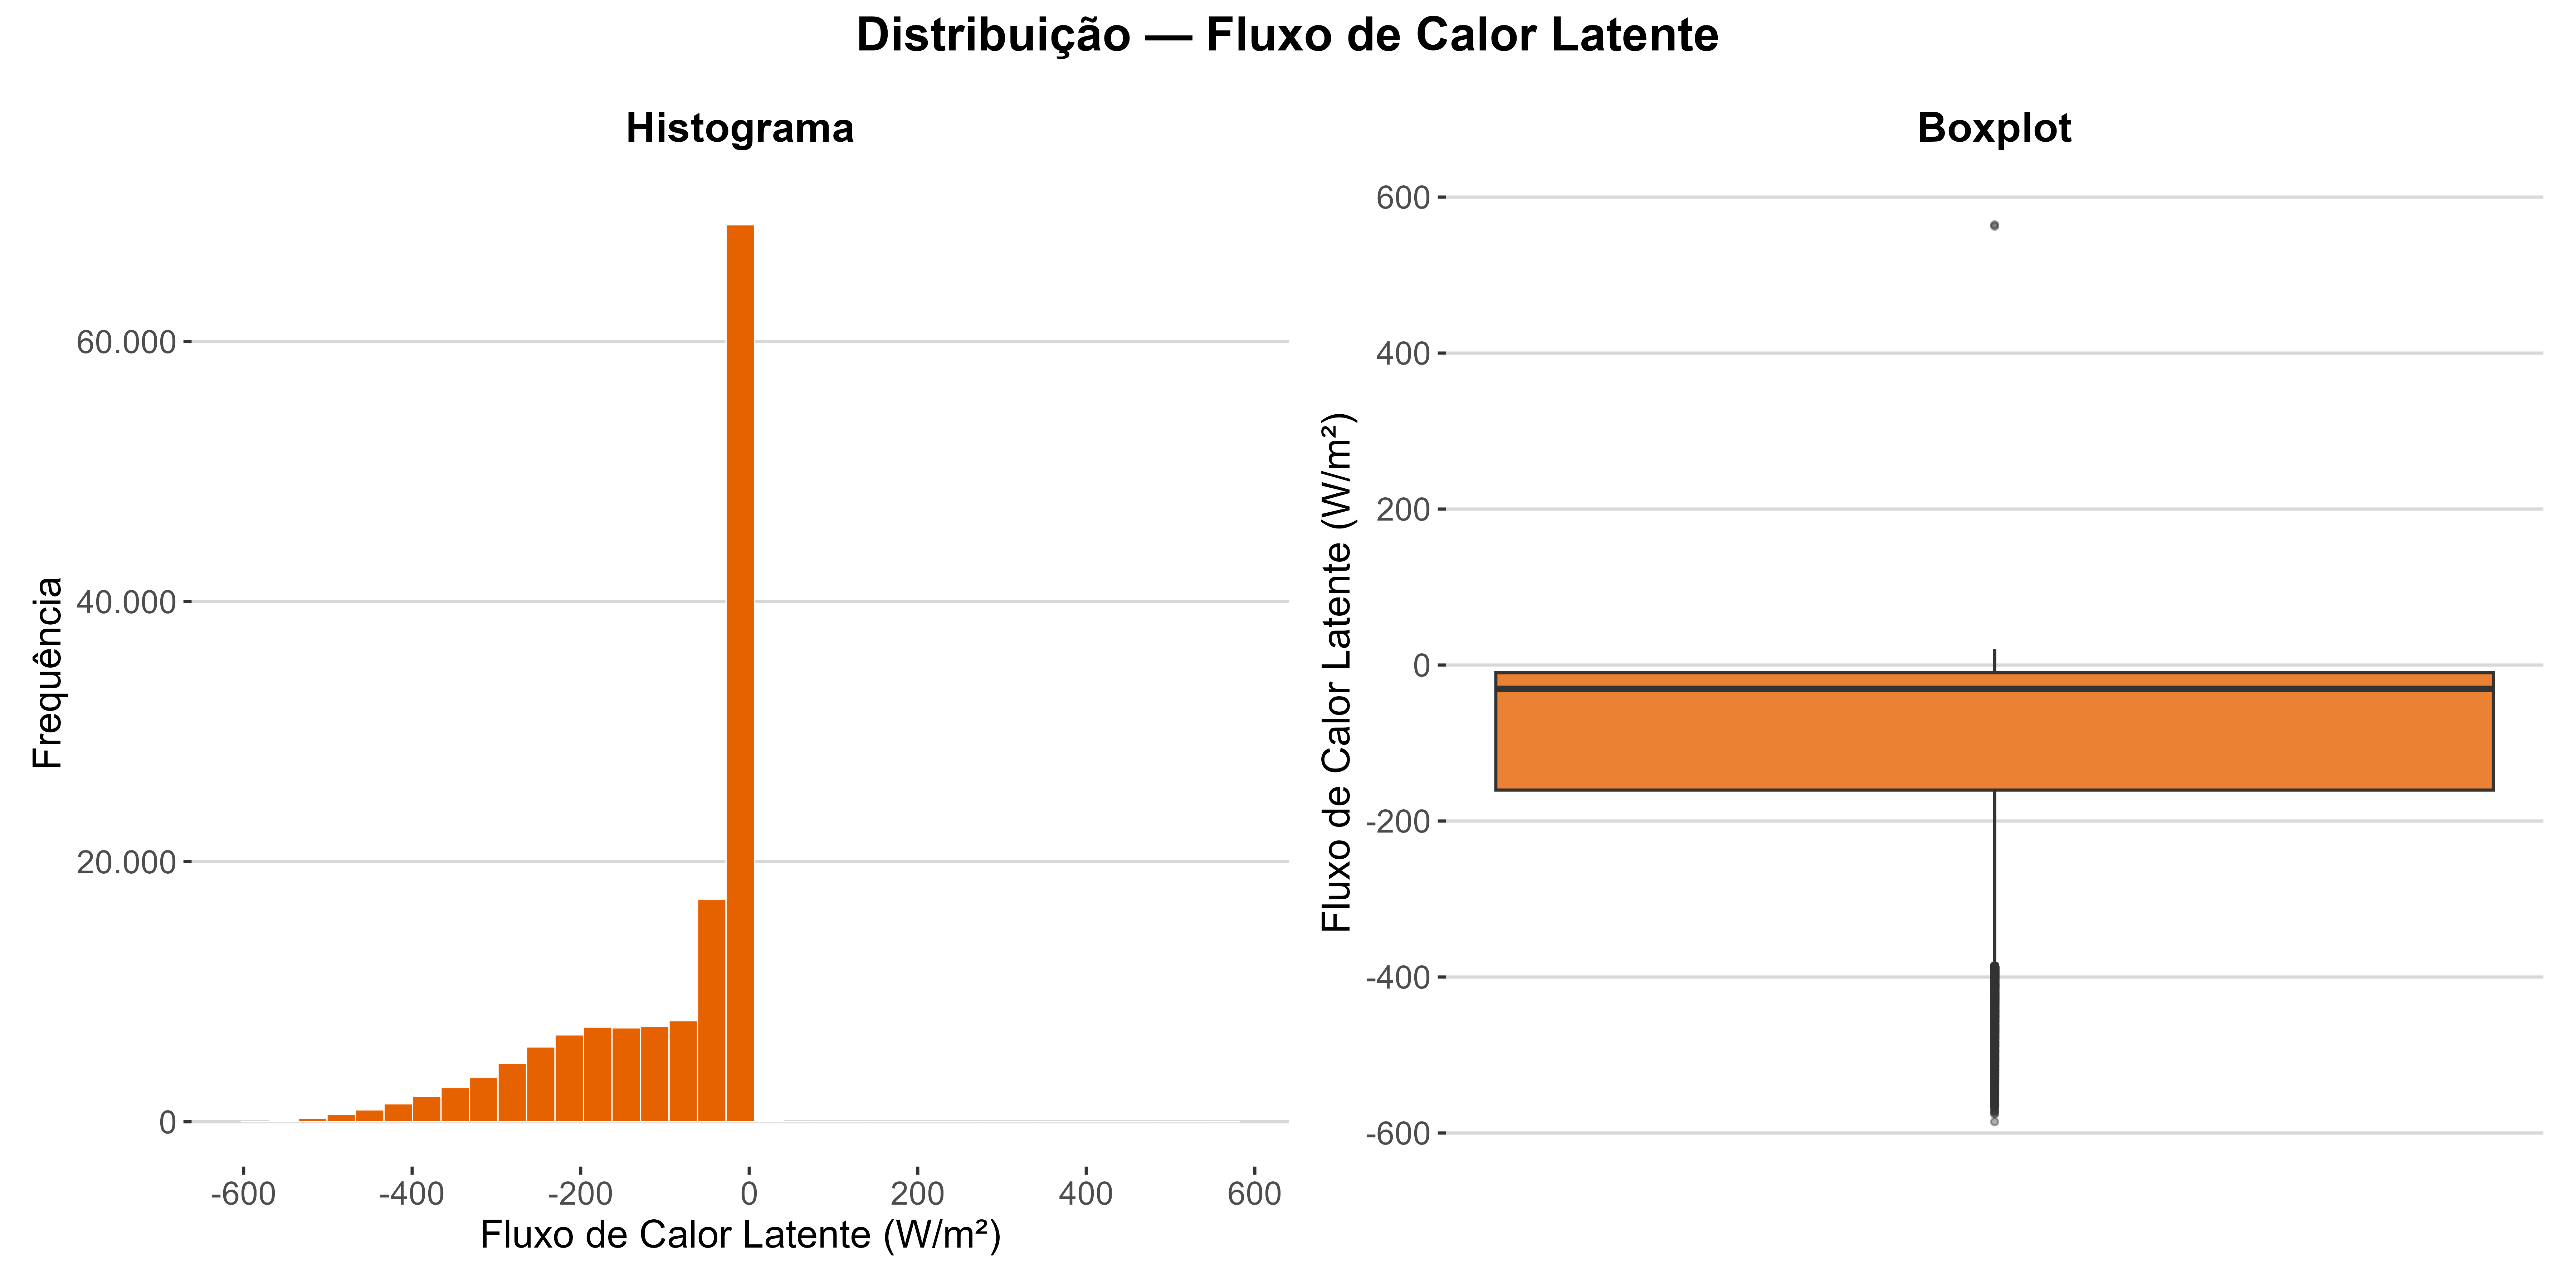
\includegraphics[keepaspectratio]{resultados/FluxoCalorLatente/04_fluxocalorlatente_distribuicao.png}}

}

\caption{Distribuição do Fluxo de Calor Latente}

\end{figure}%

\paragraph{Principais Achados}\label{principais-achados-9}

O fluxo de calor latente (evapotranspiração) é consistentemente
\textbf{negativo} e apresenta a maior amplitude entre os fluxos
energéticos. Os picos são mais intensos no verão, quando a combinação de
alta temperatura, umidade e radiação solar favorece a evaporação. A
série mensal evidencia com clareza a sazonalidade, com mínimos no
inverno seco.

A distribuição é assimétrica à esquerda, com concentração de valores
baixos e cauda longa. Há a presença de valores extremos positivos que
são provaveis erros na base de dados.

Em conjunto com o fluxo de calor sensível, essa variável compõe o
balanço de energia da superfície e deve ser relevante como preditor da
temperatura do ar.

\subsubsection{Vento Leste-Oeste}\label{vento-leste-oeste}

\begin{figure}[H]

{\centering \pandocbounded{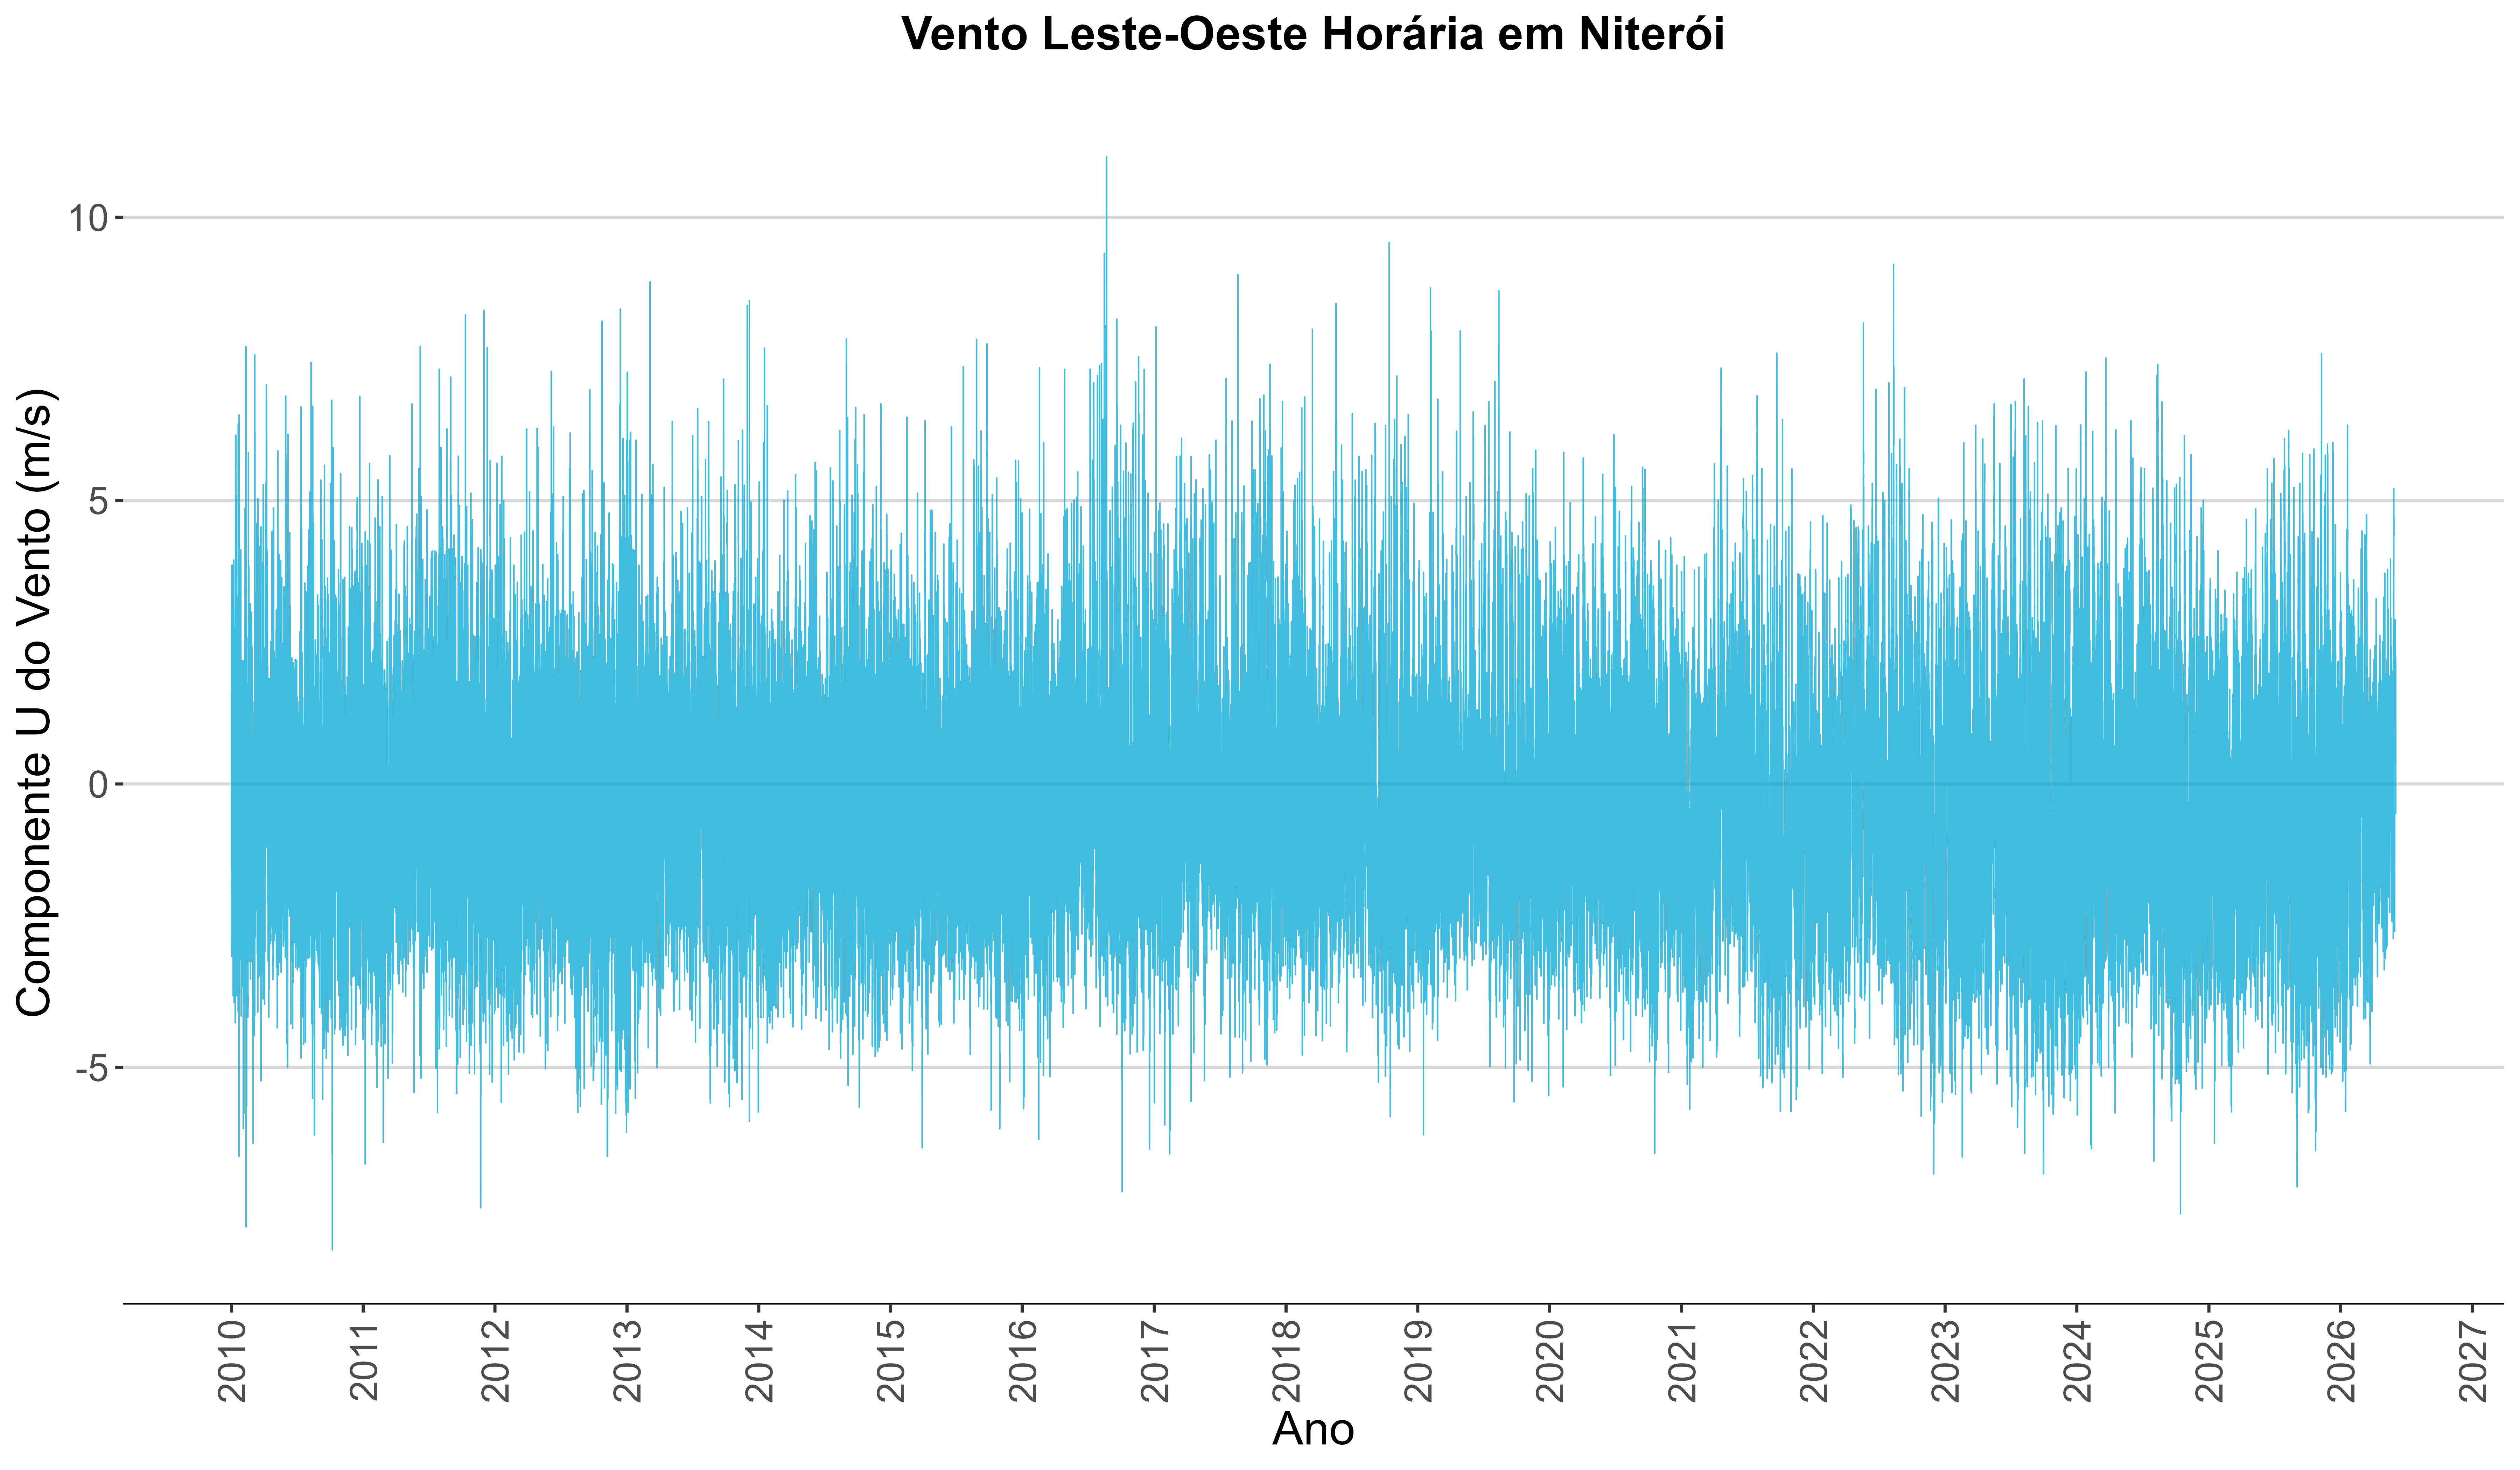
\includegraphics[keepaspectratio]{resultados/VentoU/00_ventou_horario.png}}

}

\caption{Vento Leste-Oeste Horário}

\end{figure}%

\begin{figure}[H]

{\centering \pandocbounded{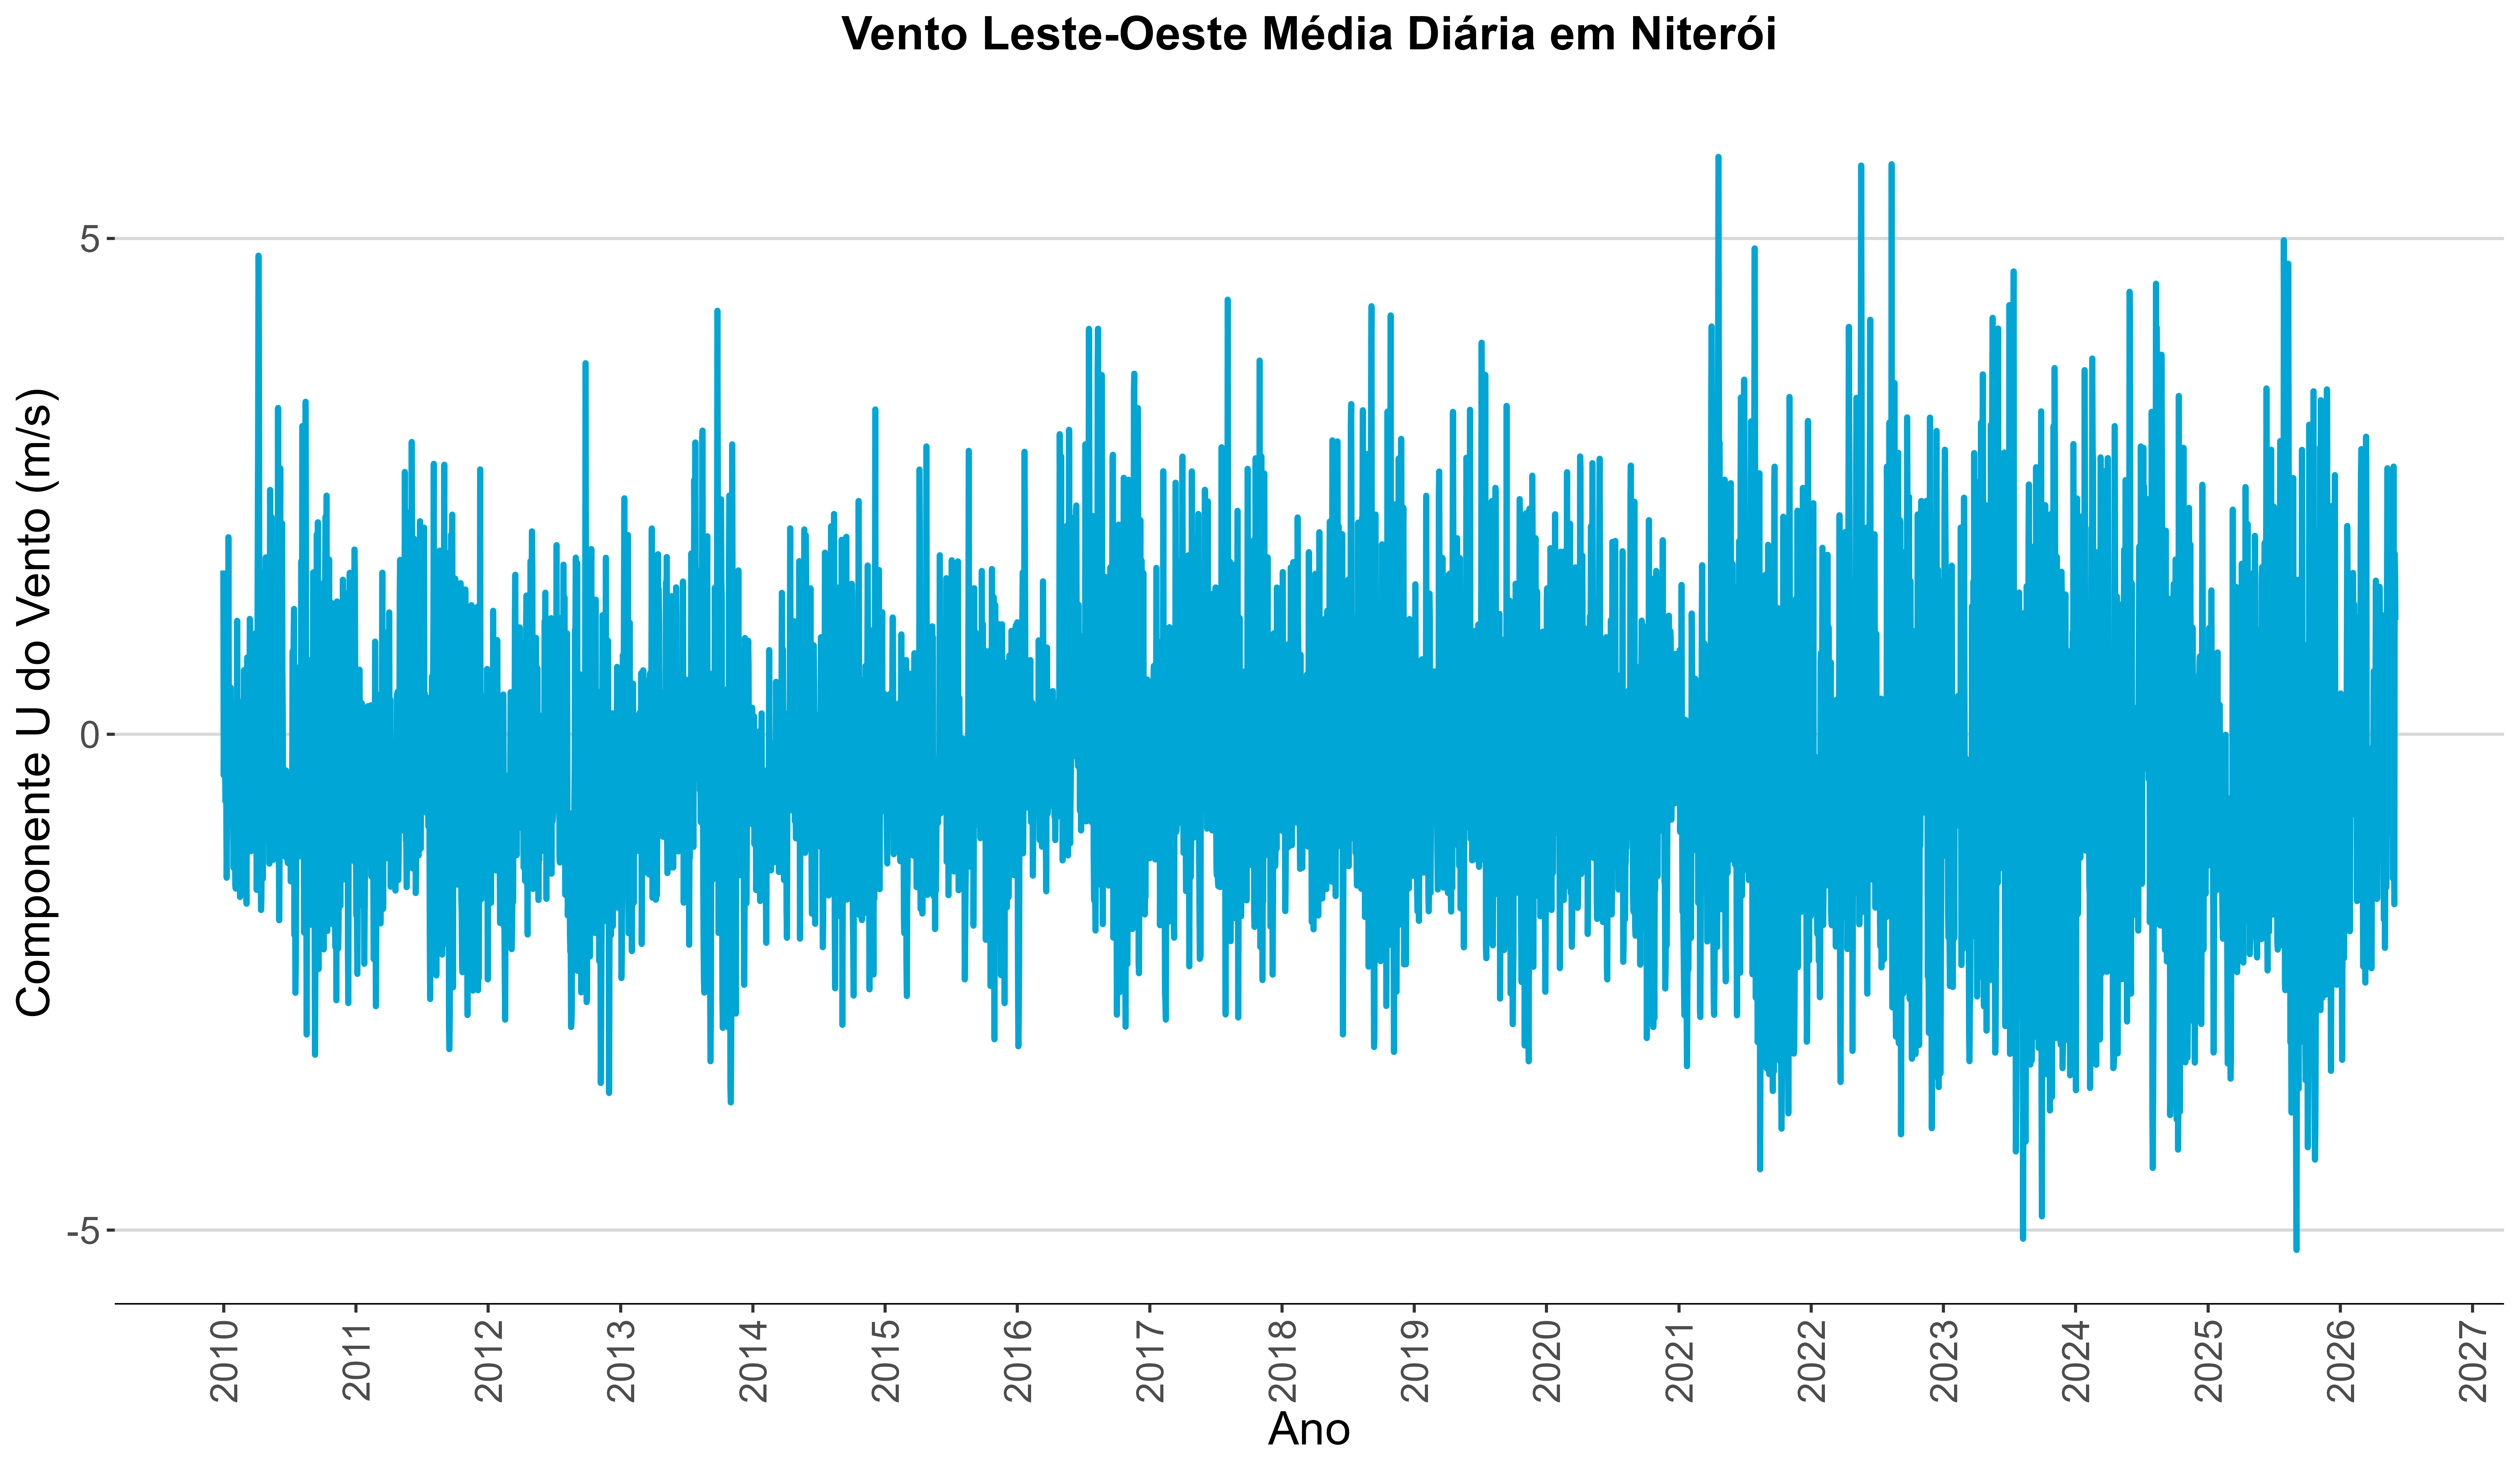
\includegraphics[keepaspectratio]{resultados/VentoU/01_ventou_diario.png}}

}

\caption{Vento Leste-Oeste Médio Diário}

\end{figure}%

\begin{figure}[H]

{\centering \pandocbounded{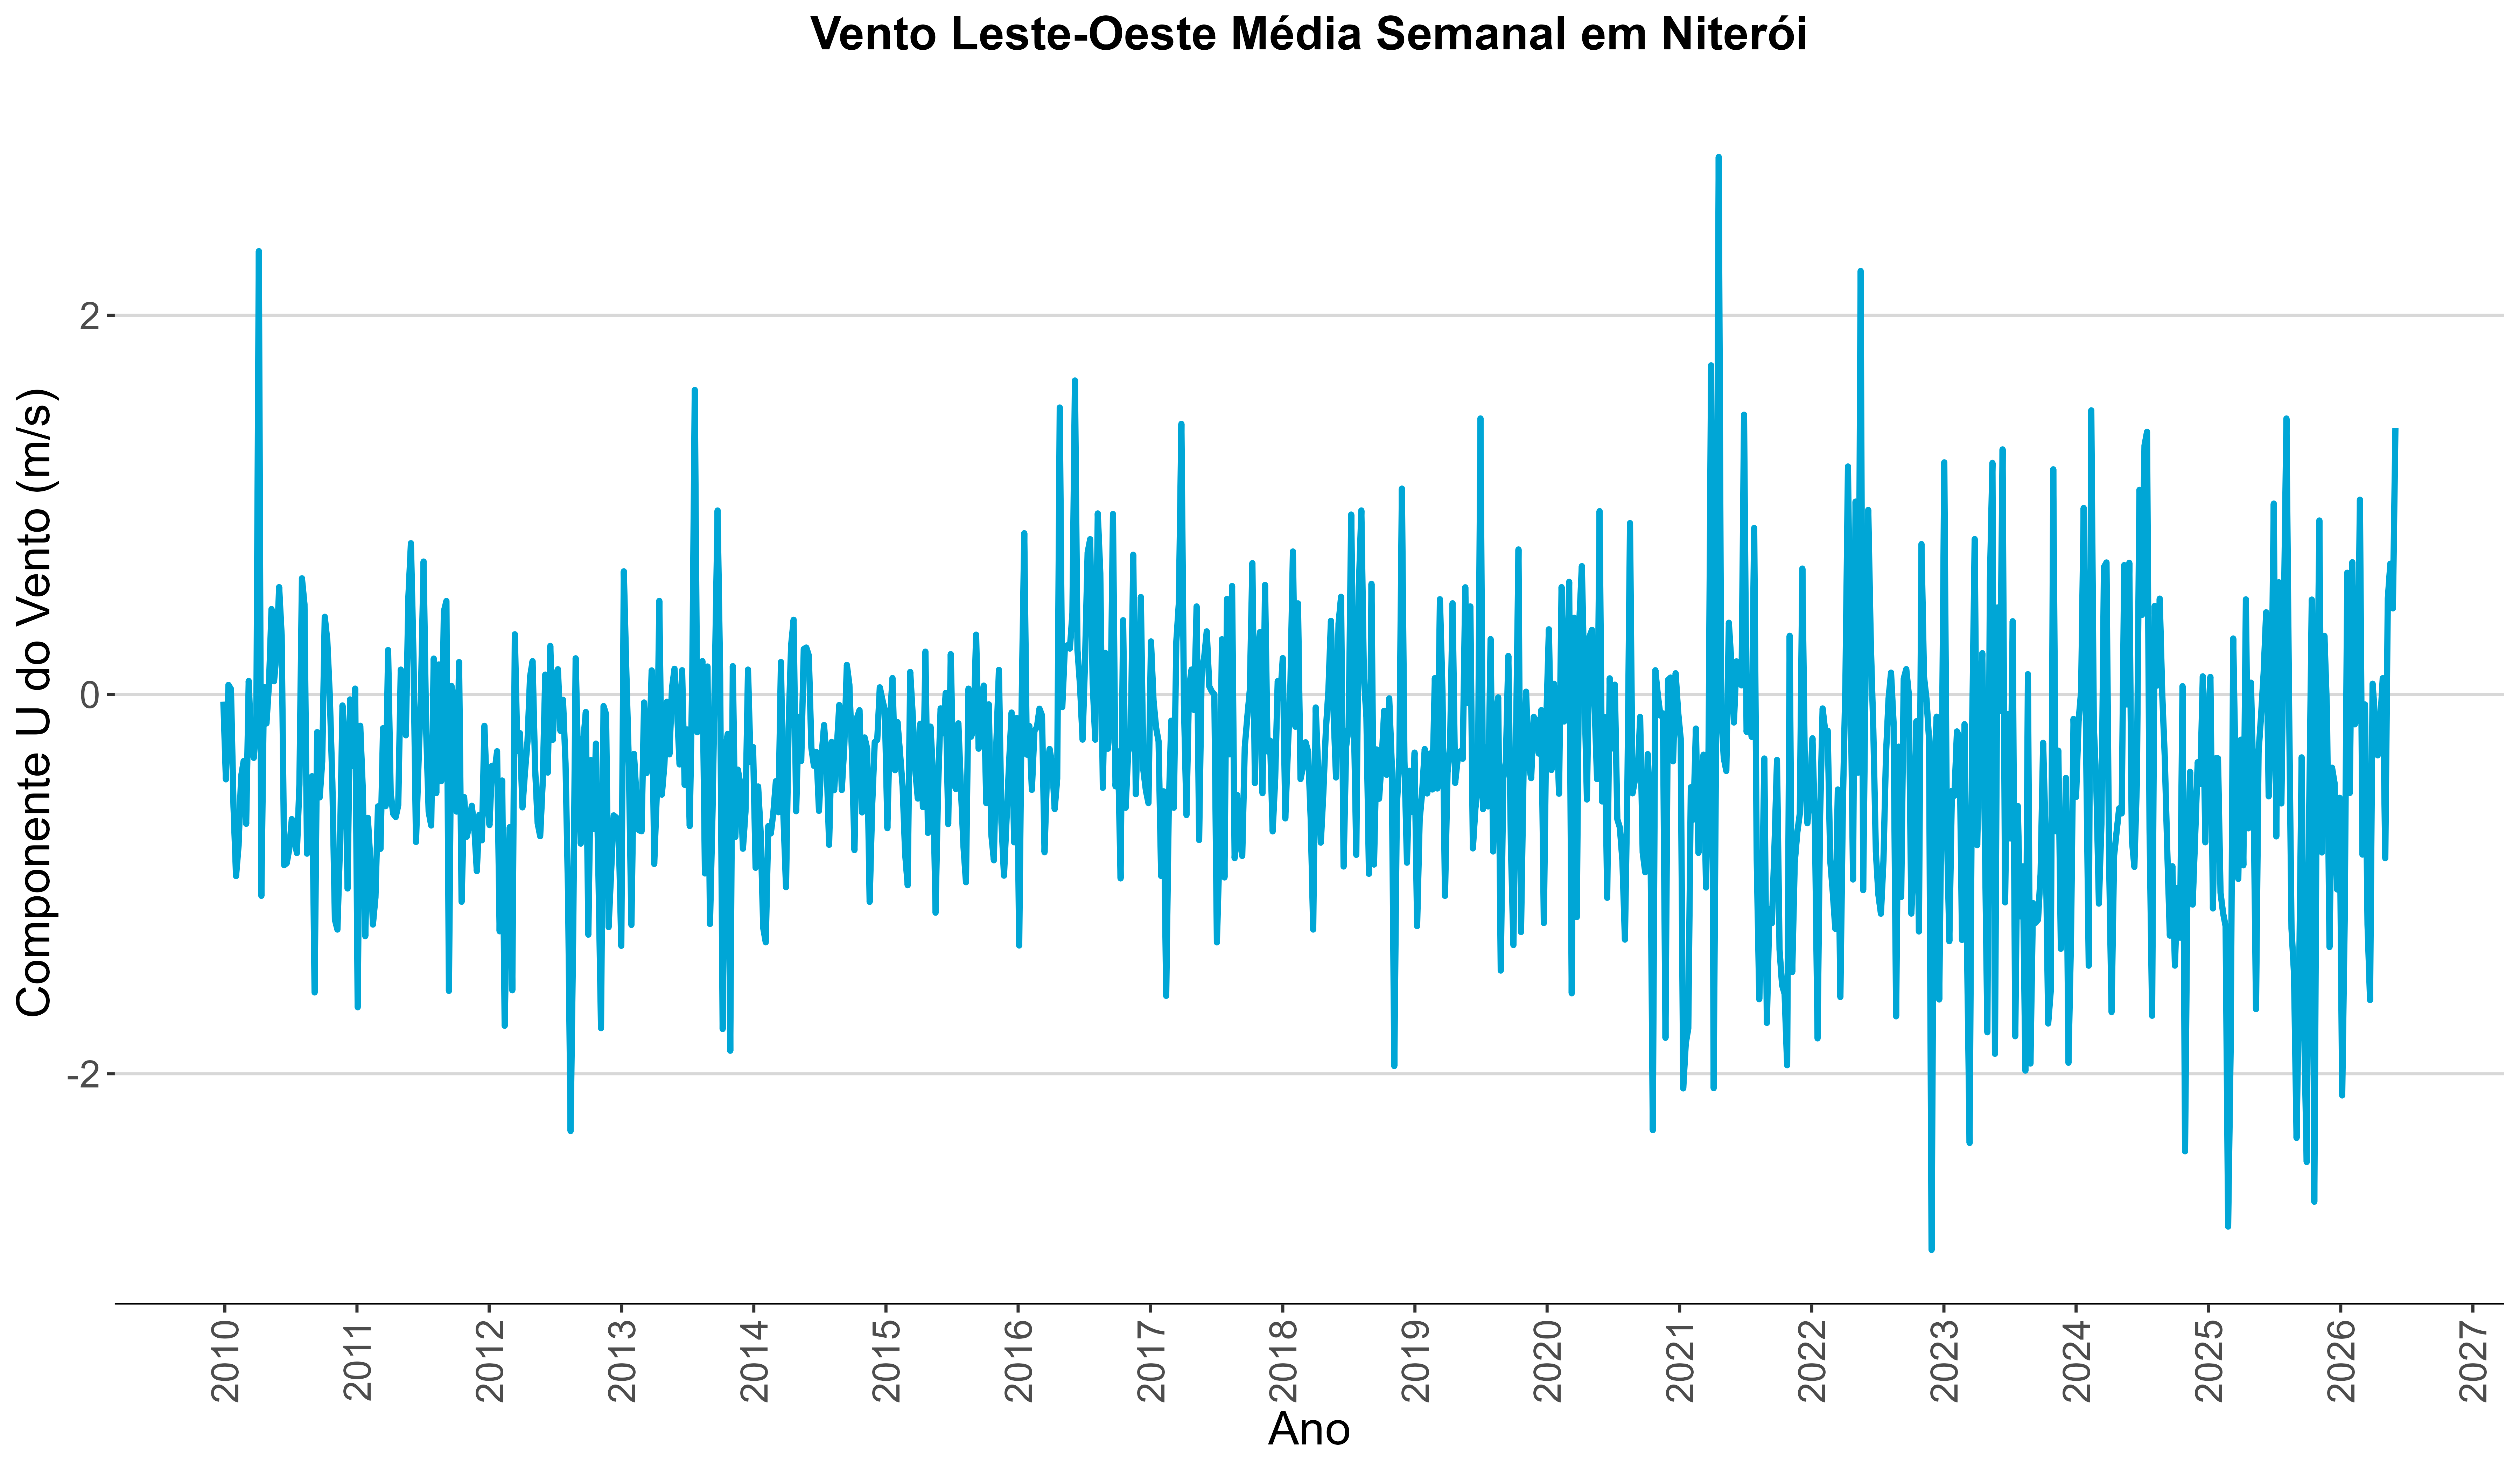
\includegraphics[keepaspectratio]{resultados/VentoU/02_ventou_semanal.png}}

}

\caption{Vento Leste-Oeste Médio Semanal}

\end{figure}%

\begin{figure}[H]

{\centering \pandocbounded{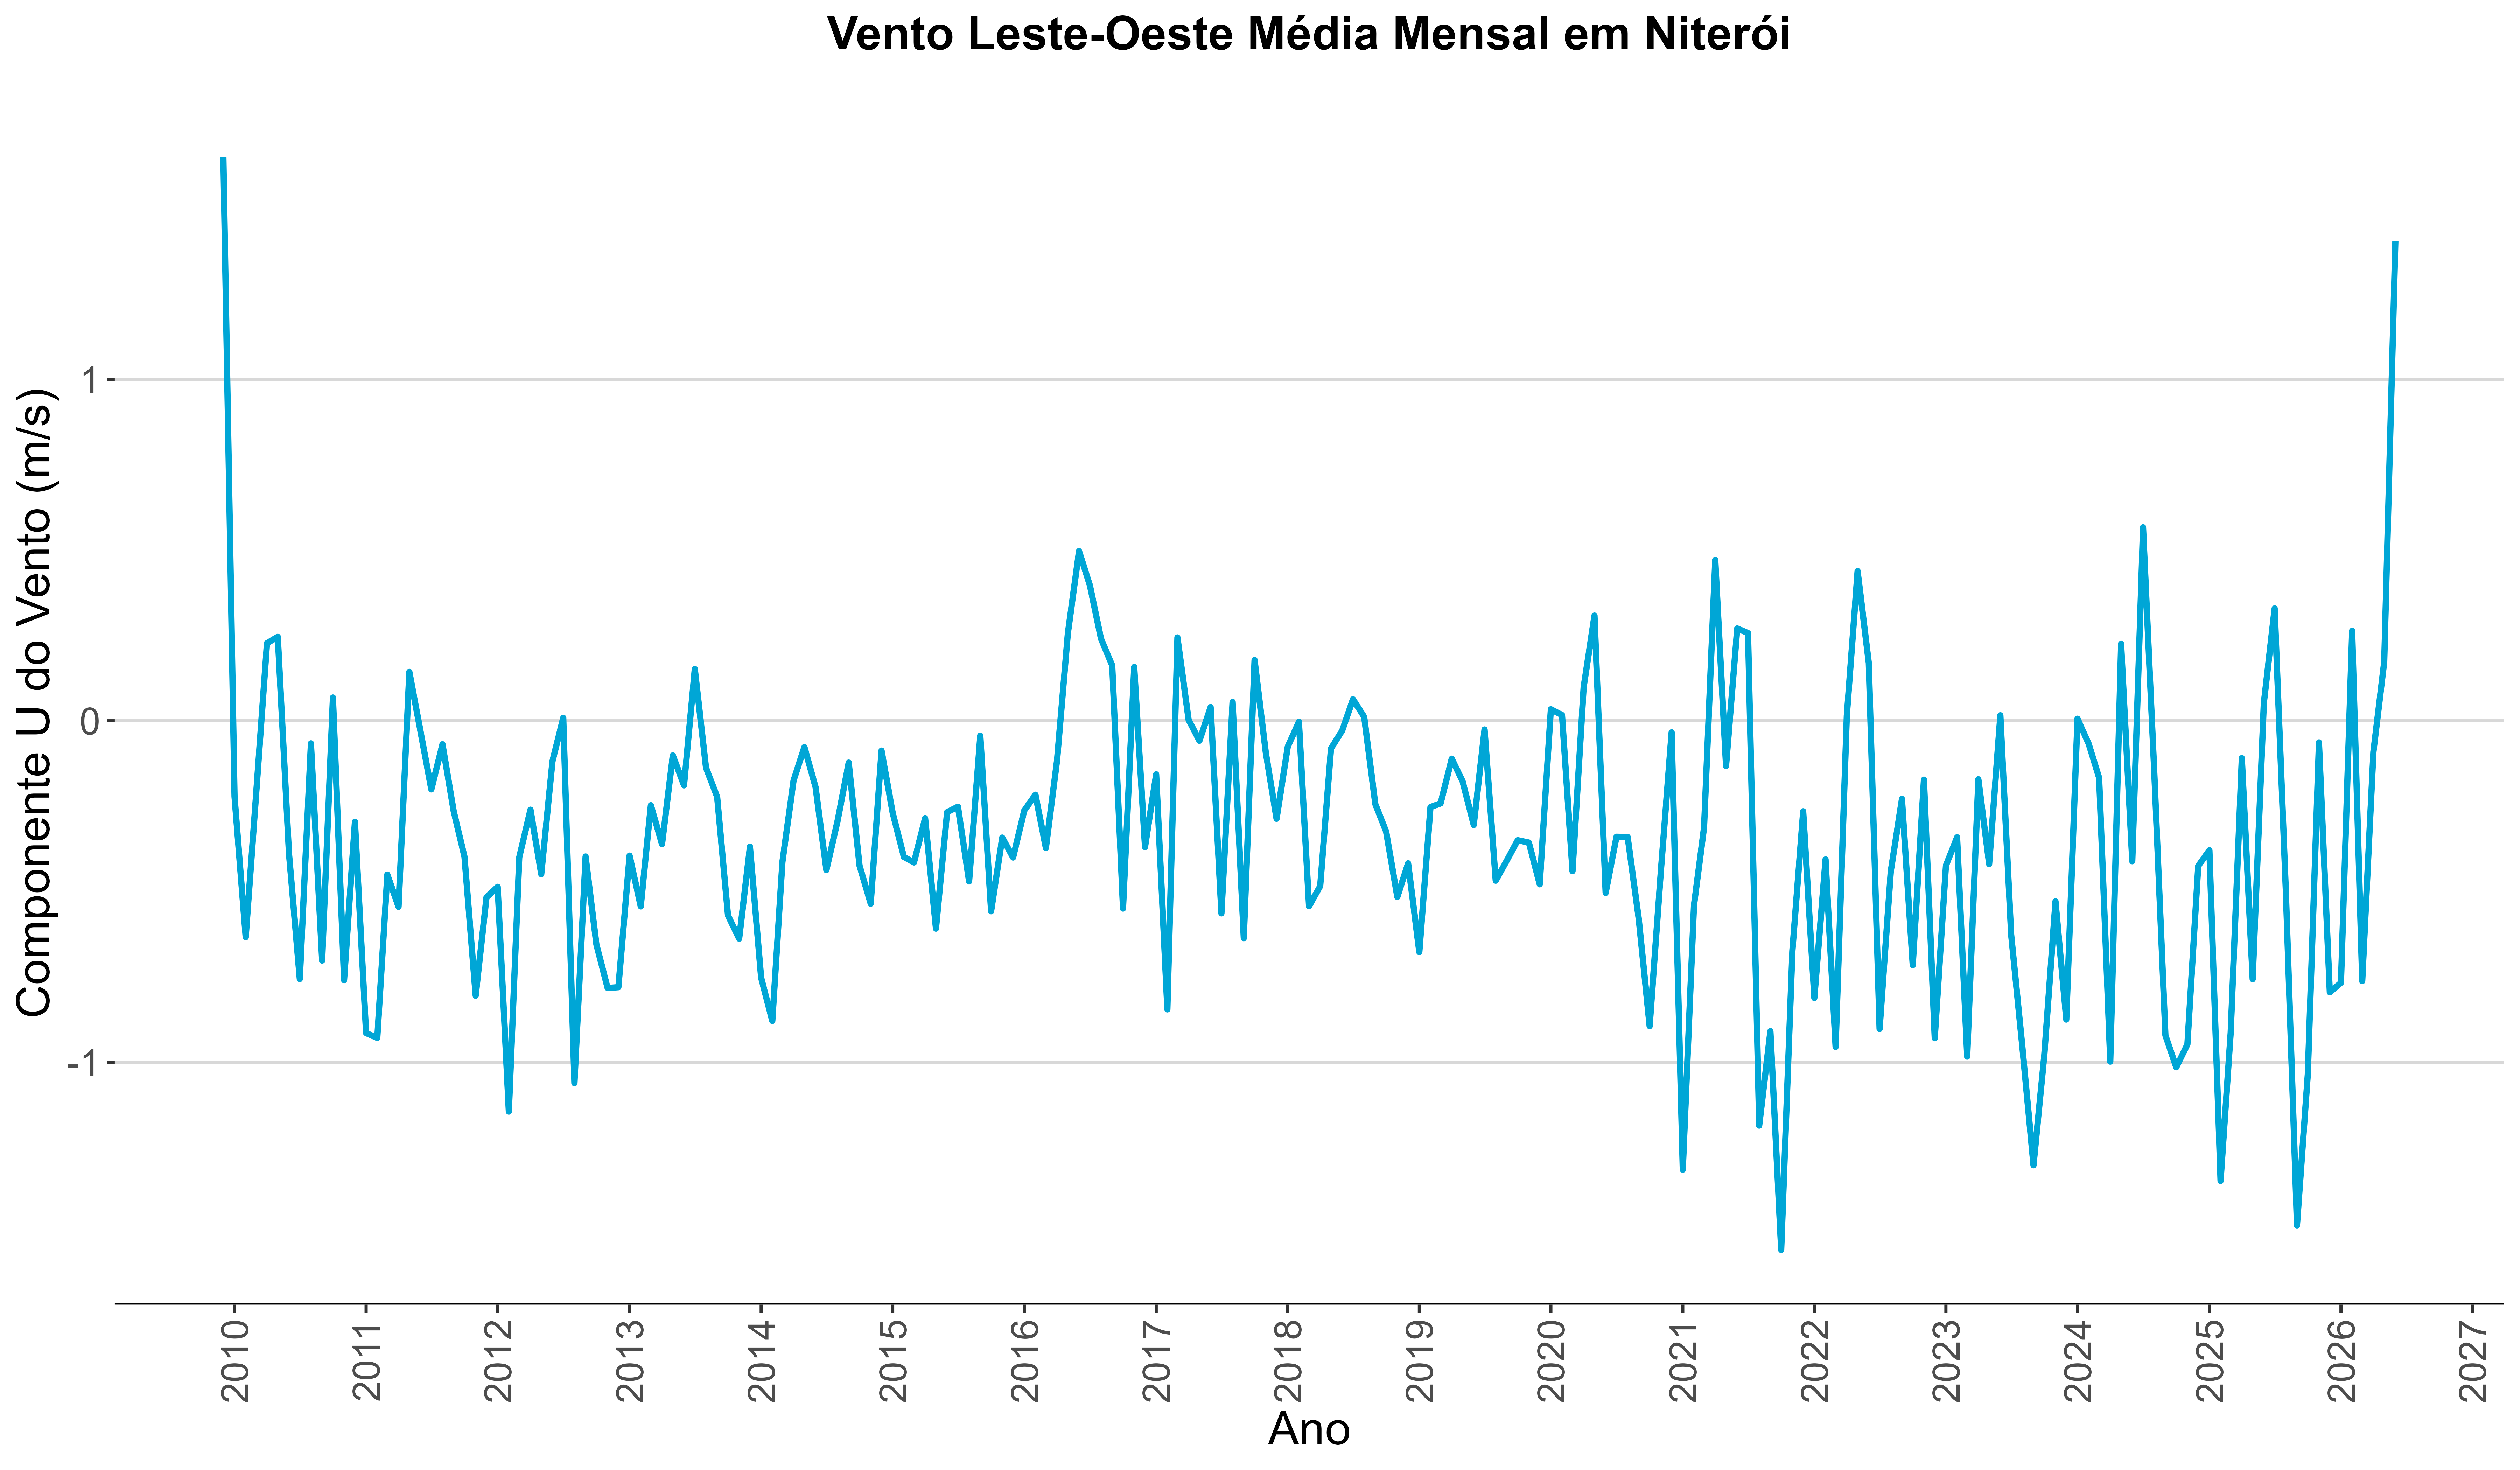
\includegraphics[keepaspectratio]{resultados/VentoU/03_ventou_mensal.png}}

}

\caption{Vento Leste-Oeste Médio Mensal}

\end{figure}%

\begin{figure}[H]

{\centering \pandocbounded{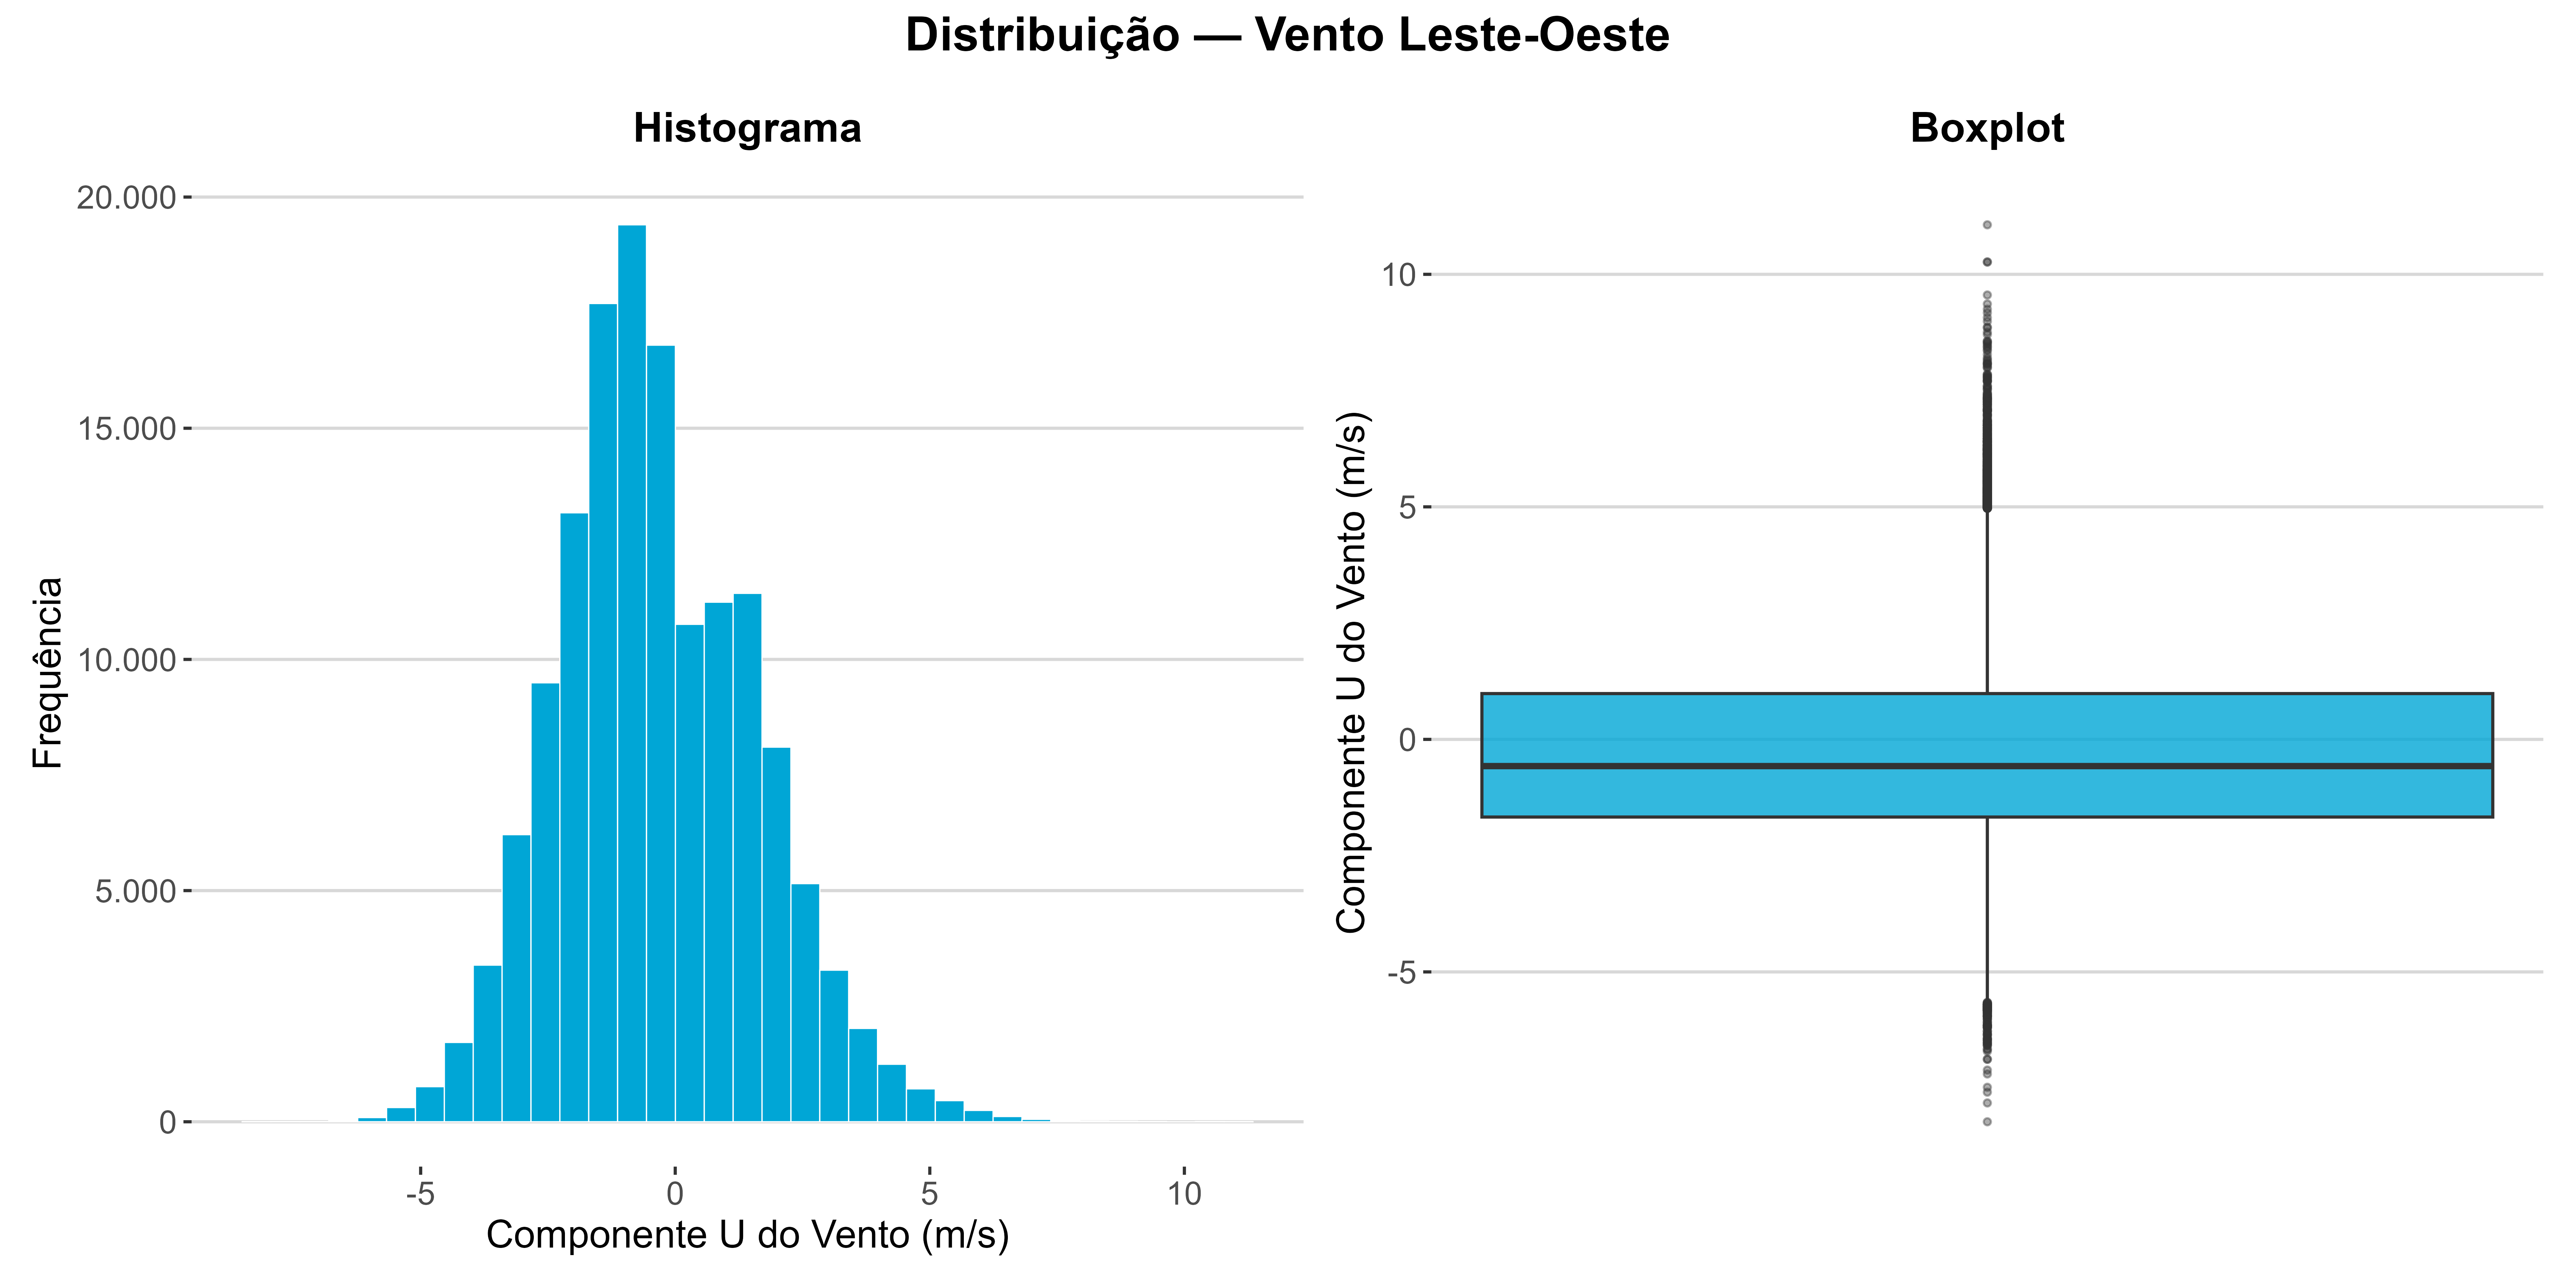
\includegraphics[keepaspectratio]{resultados/VentoU/04_ventou_distribuicao.png}}

}

\caption{Distribuição do Vento Leste-Oeste}

\end{figure}%

\paragraph{Principais Achados}\label{principais-achados-10}

A componente U do vento oscila em torno de zero, com \textbf{leve
predominância de valores negativos} (vento de leste), consistente com a
circulação dos alísios e a brisa marítima predominante em Niterói. A
série não apresenta tendência temporal, mas há maior variabilidade nos
meses de inverno e primavera.

A distribuição é centrada levemente abaixo de zero, com caudas moderadas
em ambas as direções. A ausência de valores extremos muito intensos
distingue essa componente da velocidade escalar do vento.

\subsubsection{Vento Norte-Sul}\label{vento-norte-sul}

\begin{figure}[H]

{\centering \pandocbounded{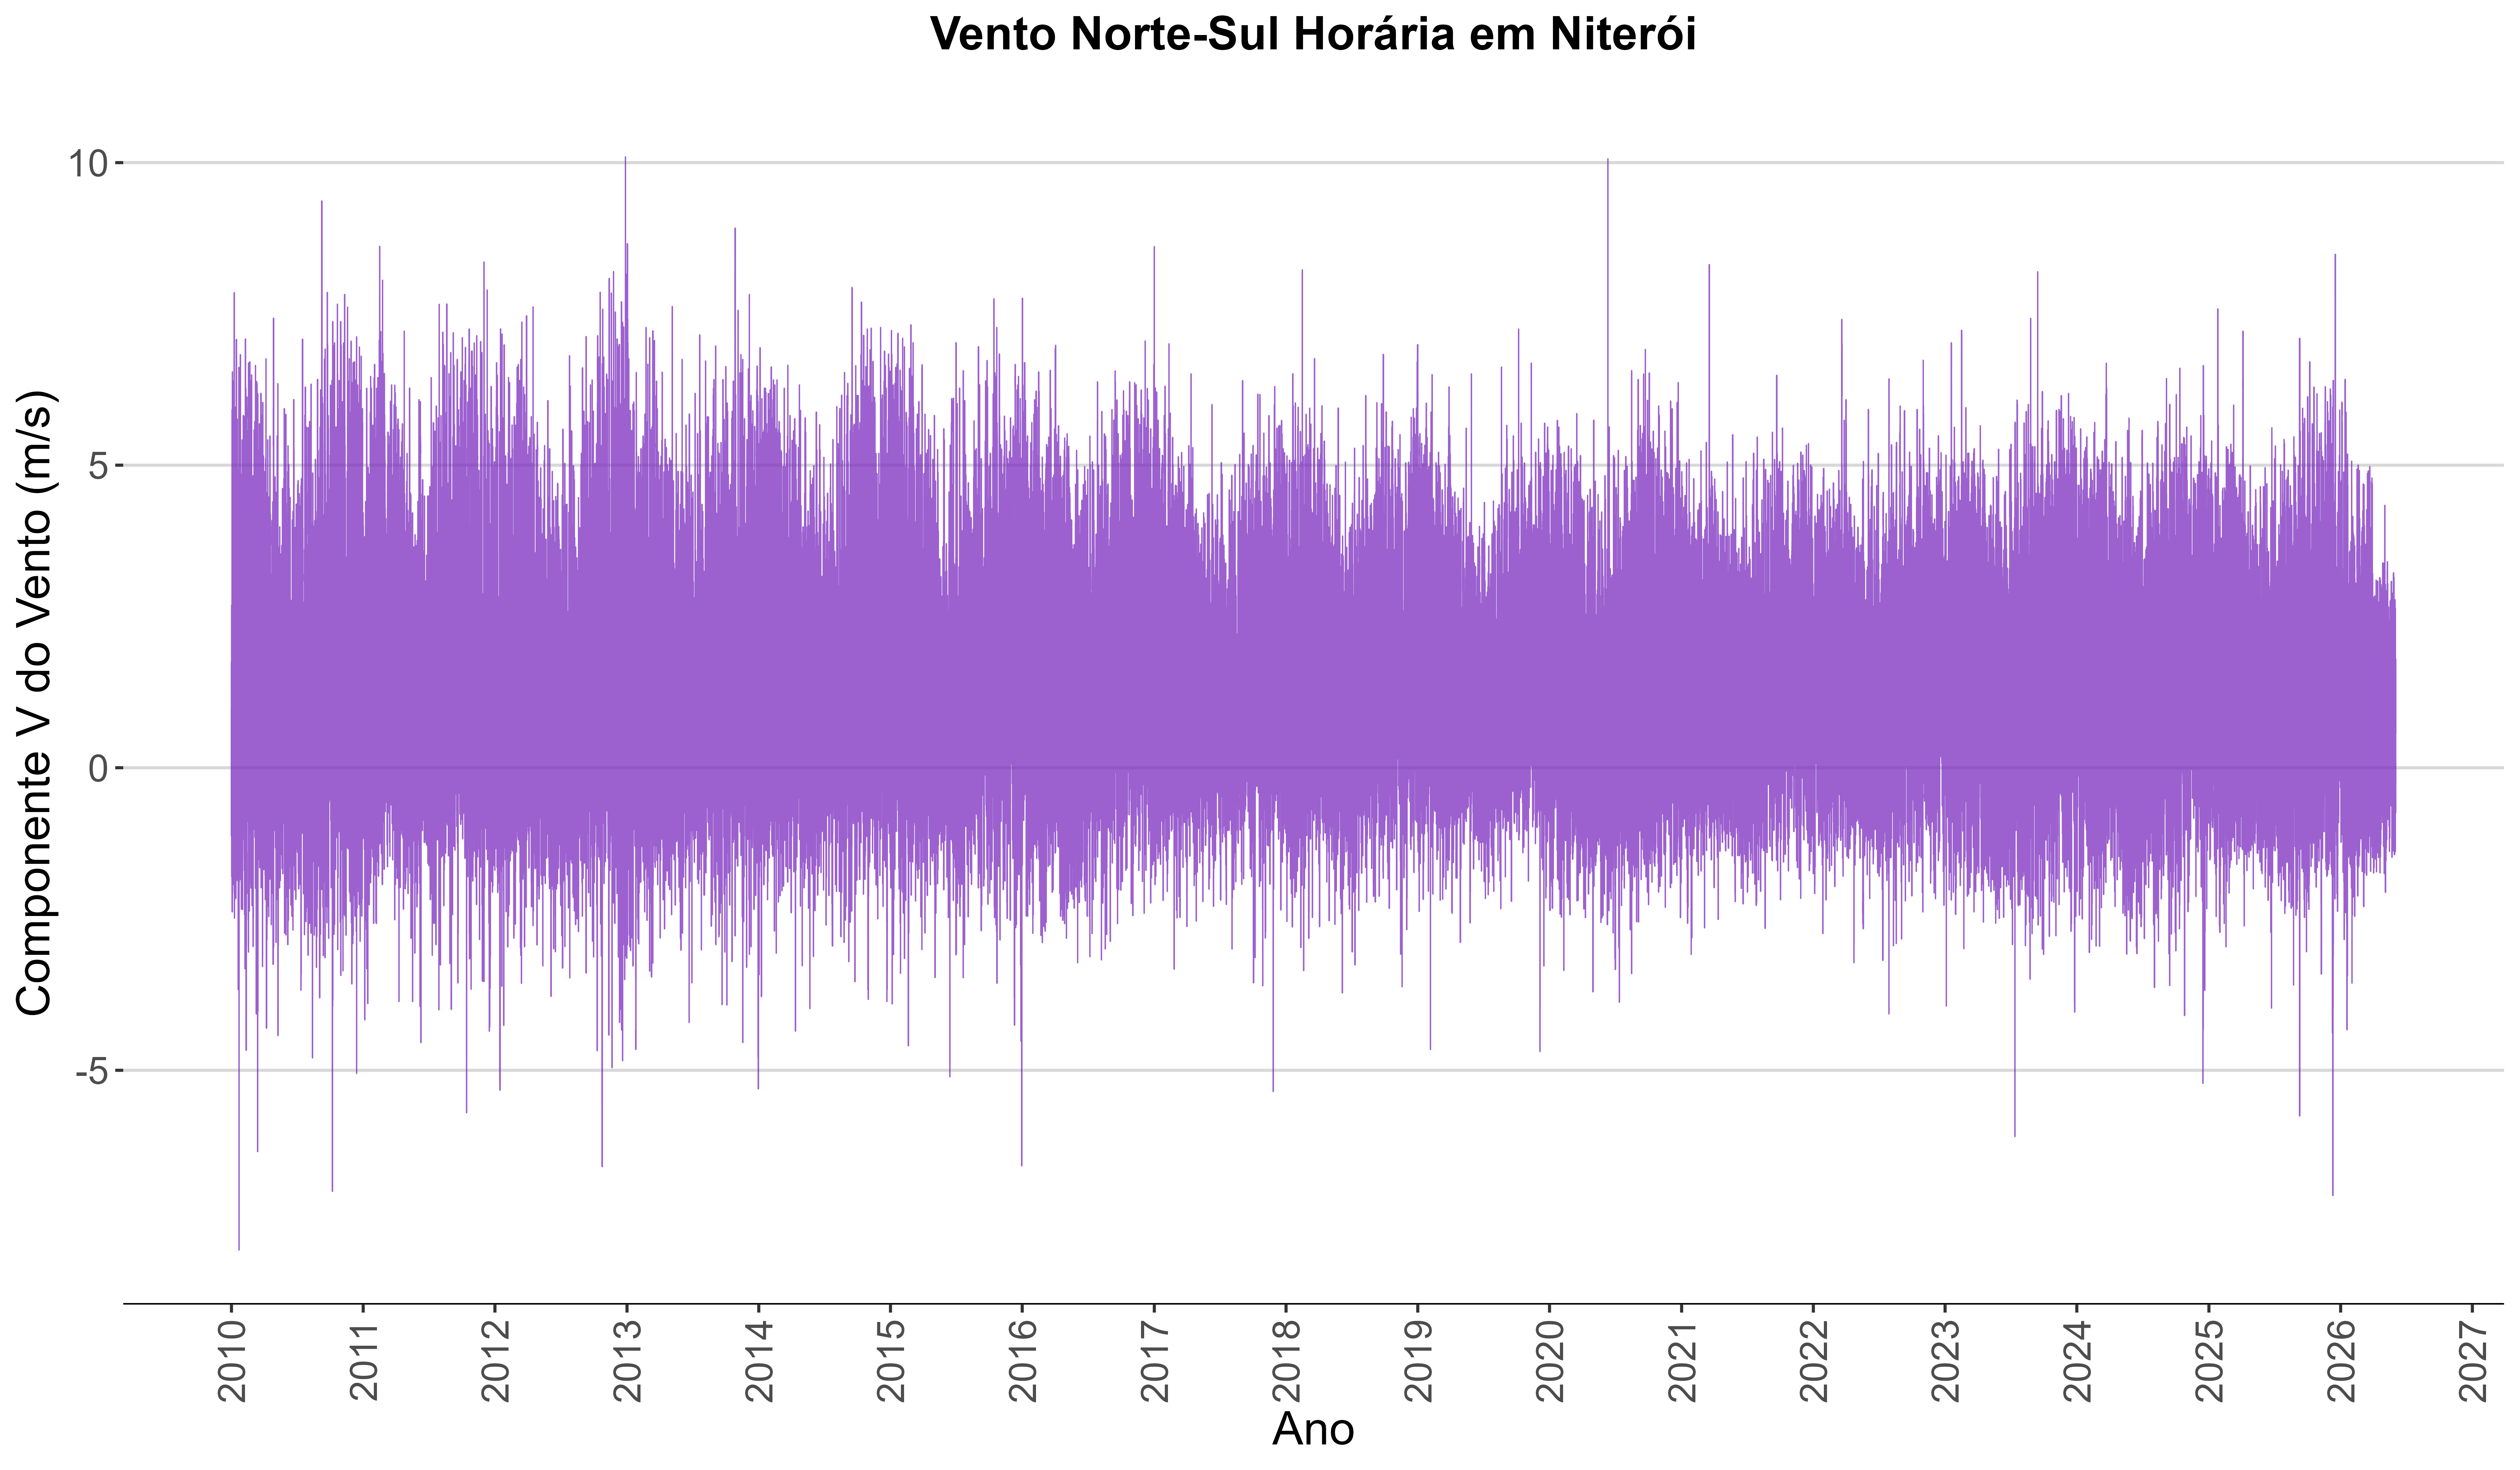
\includegraphics[keepaspectratio]{resultados/VentoV/00_ventov_horario.png}}

}

\caption{Vento Norte-Sul Horário}

\end{figure}%

\begin{figure}[H]

{\centering \pandocbounded{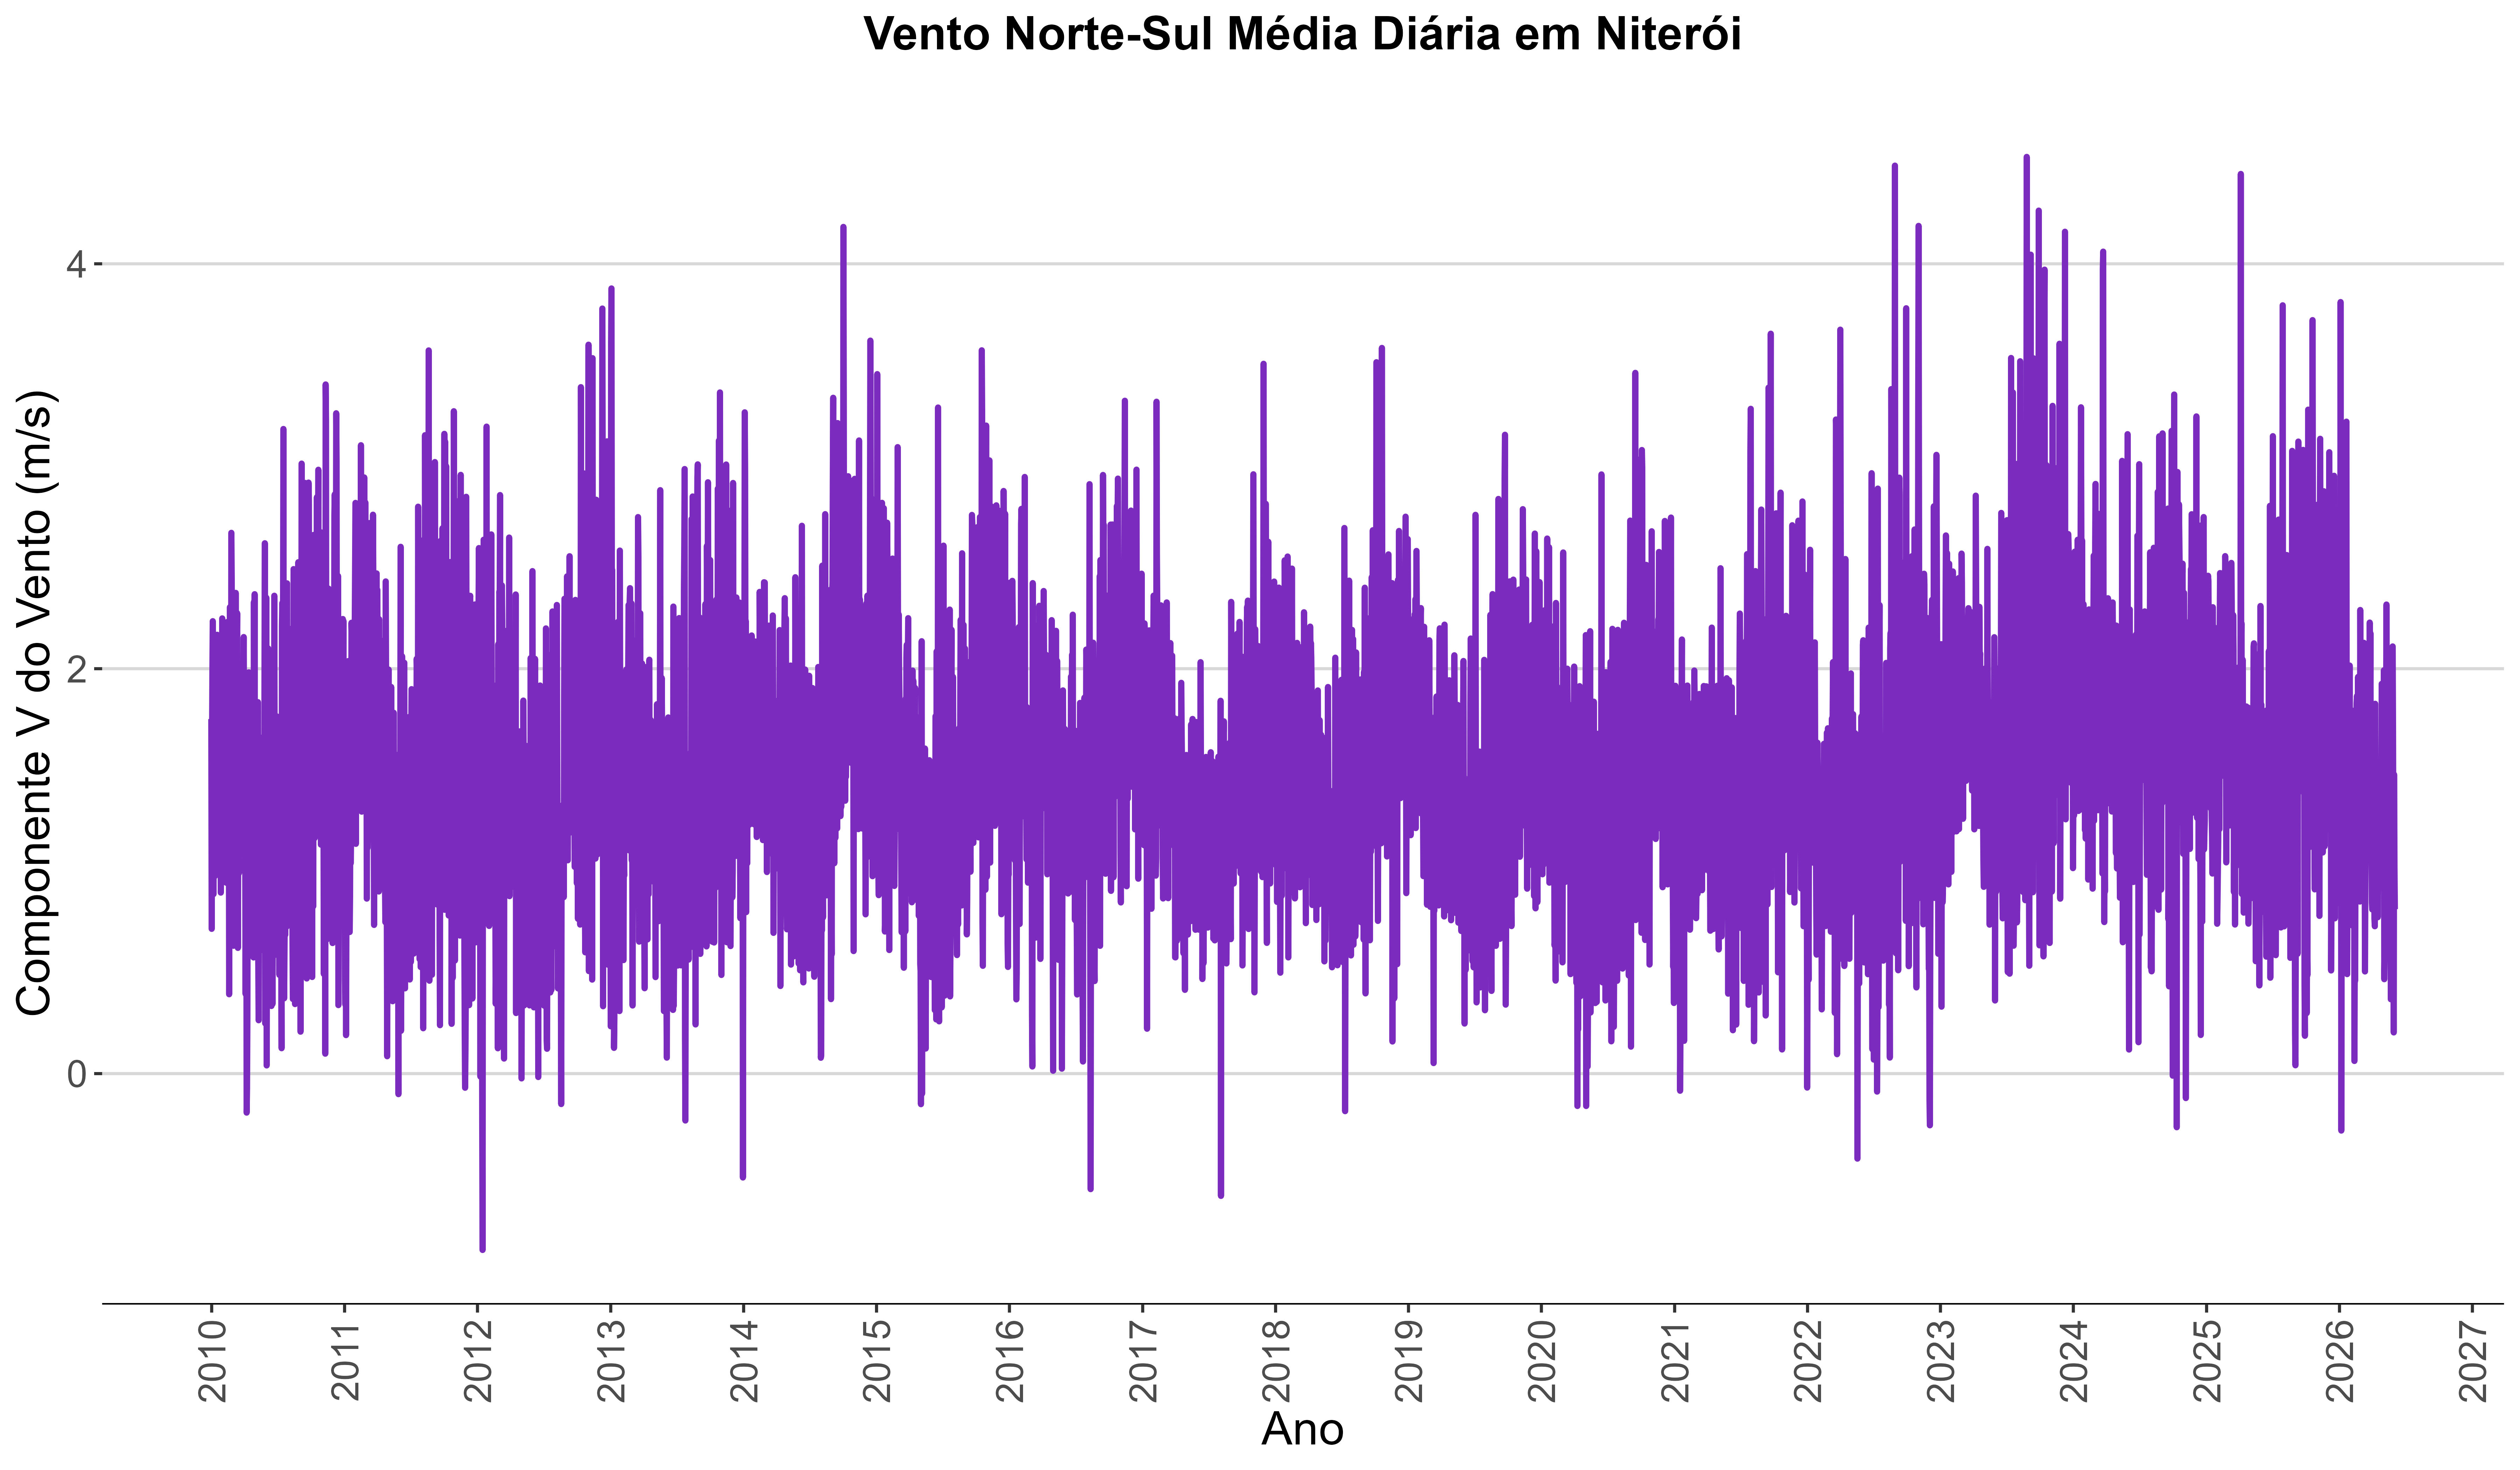
\includegraphics[keepaspectratio]{resultados/VentoV/01_ventov_diario.png}}

}

\caption{Vento Norte-Sul Médio Diário}

\end{figure}%

\begin{figure}[H]

{\centering \pandocbounded{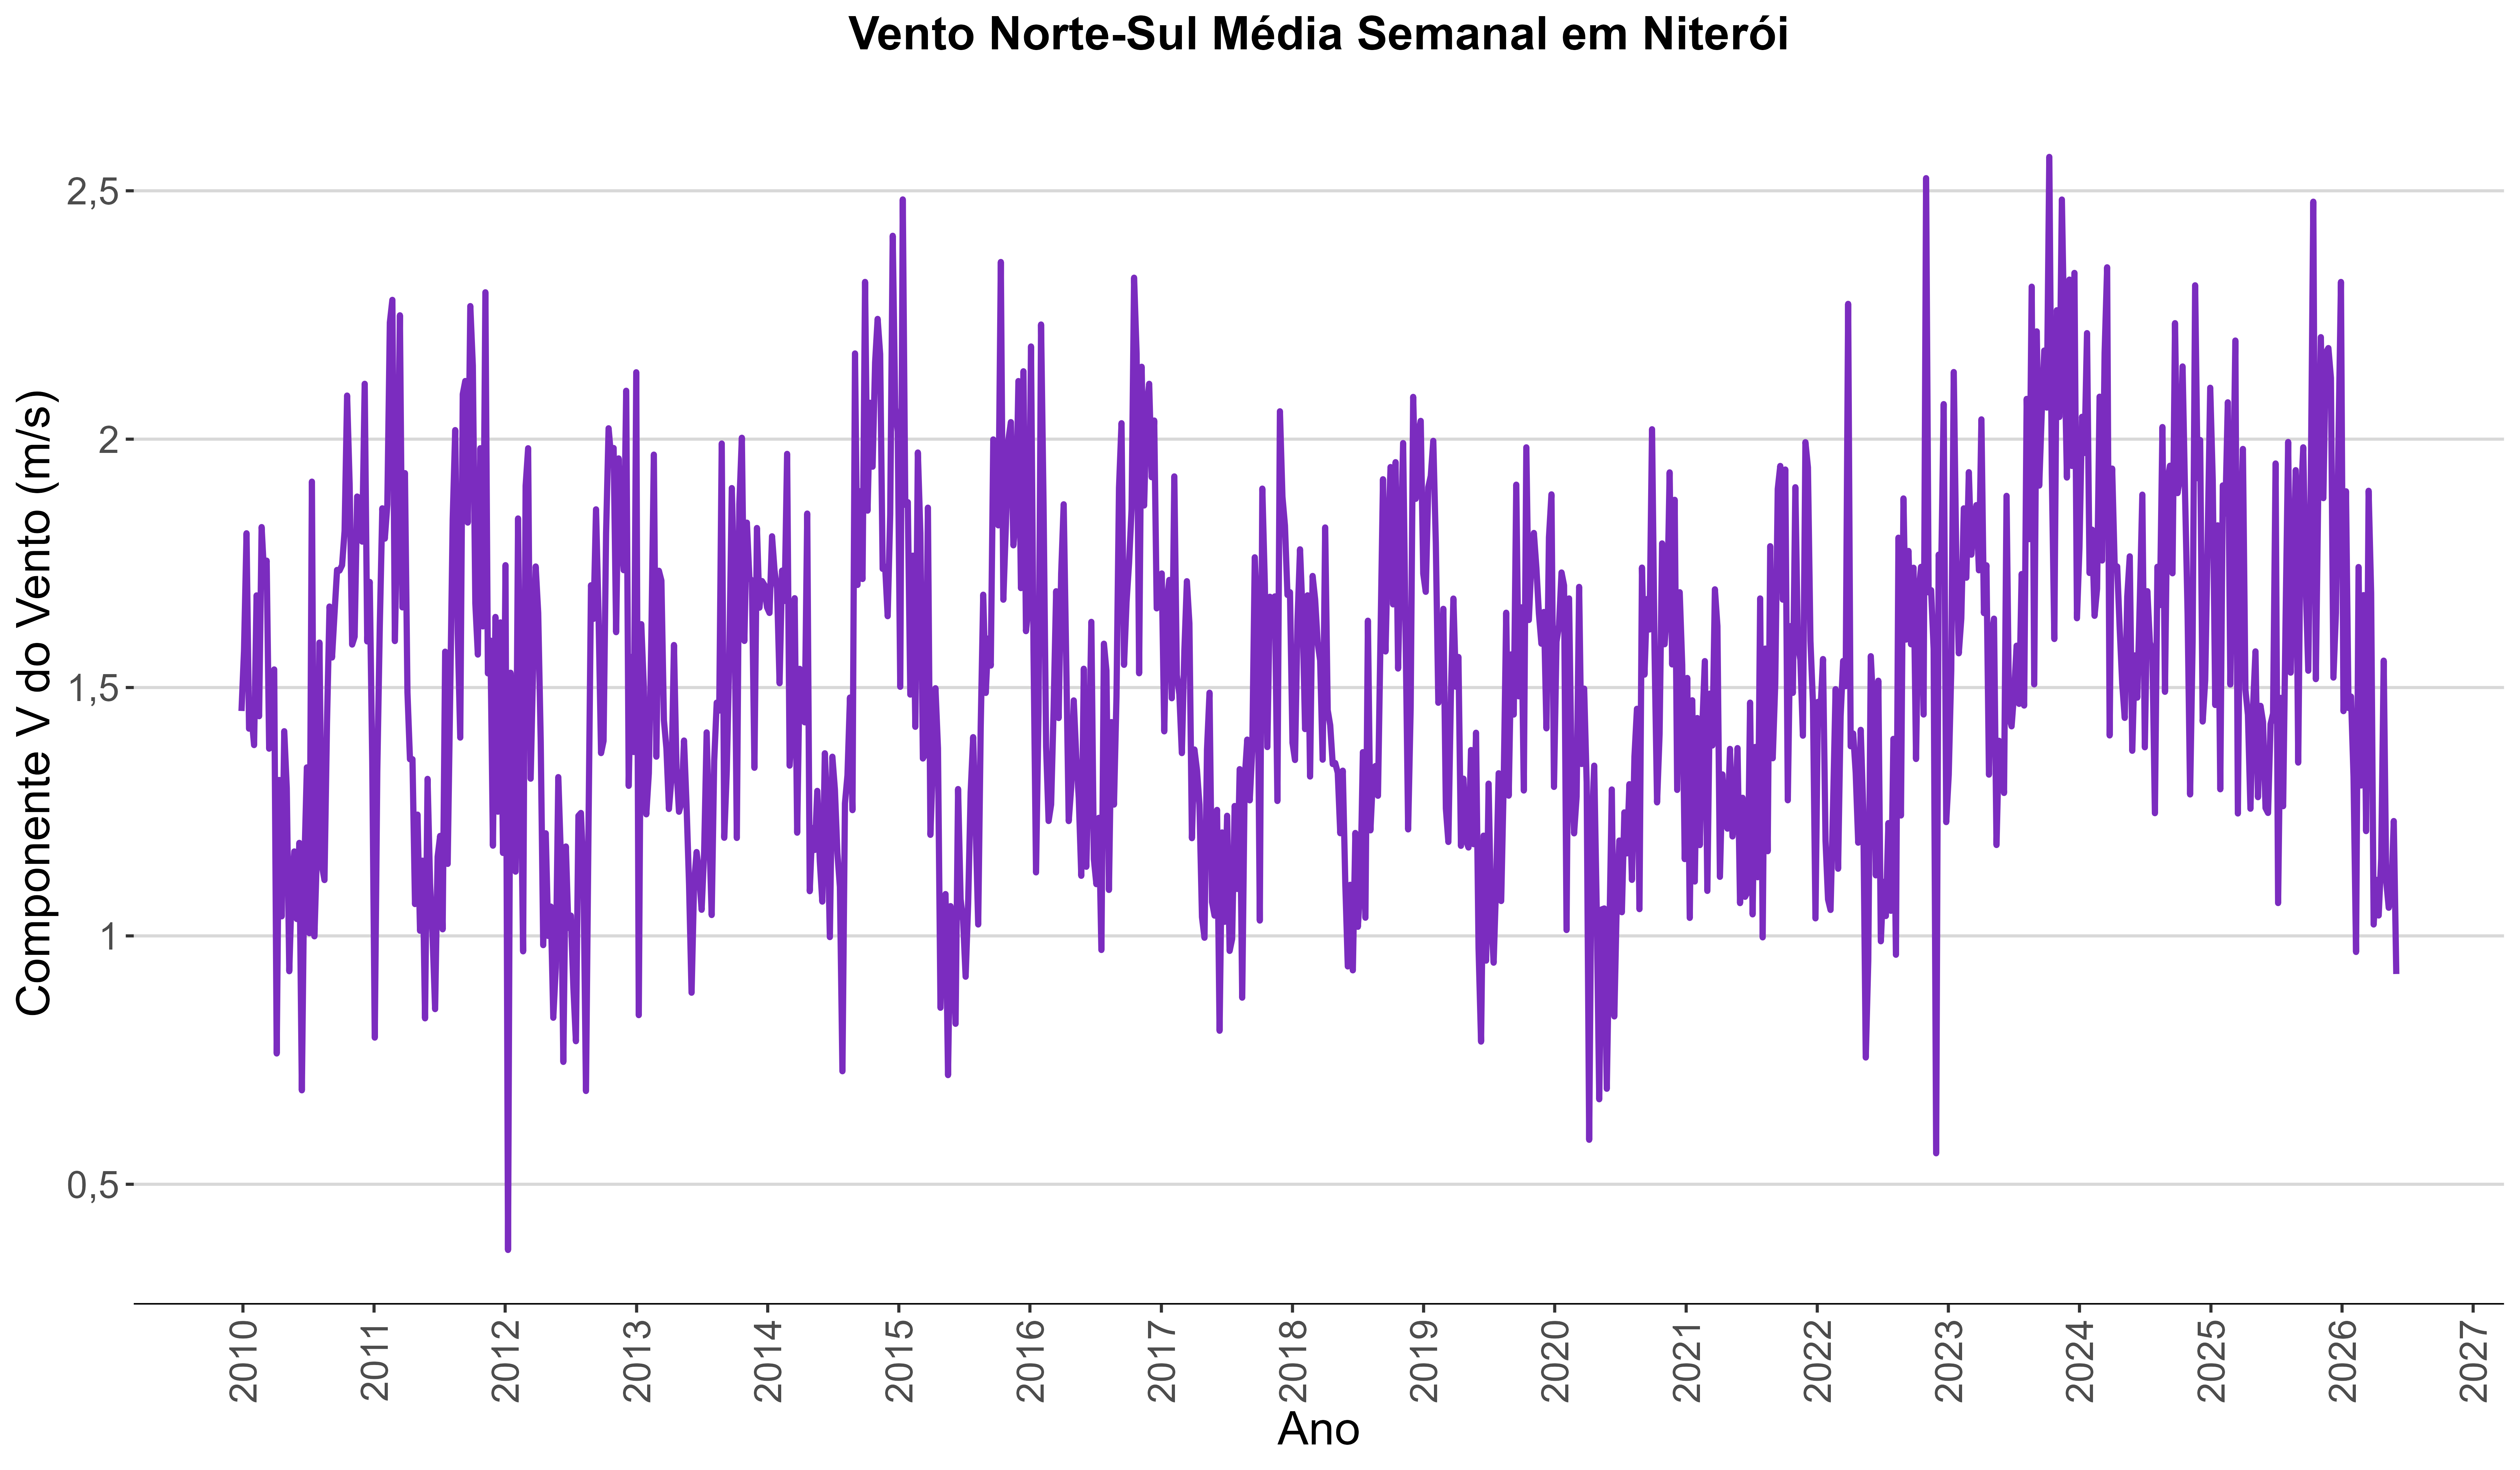
\includegraphics[keepaspectratio]{resultados/VentoV/02_ventov_semanal.png}}

}

\caption{Vento Norte-Sul Médio Semanal}

\end{figure}%

\begin{figure}[H]

{\centering \pandocbounded{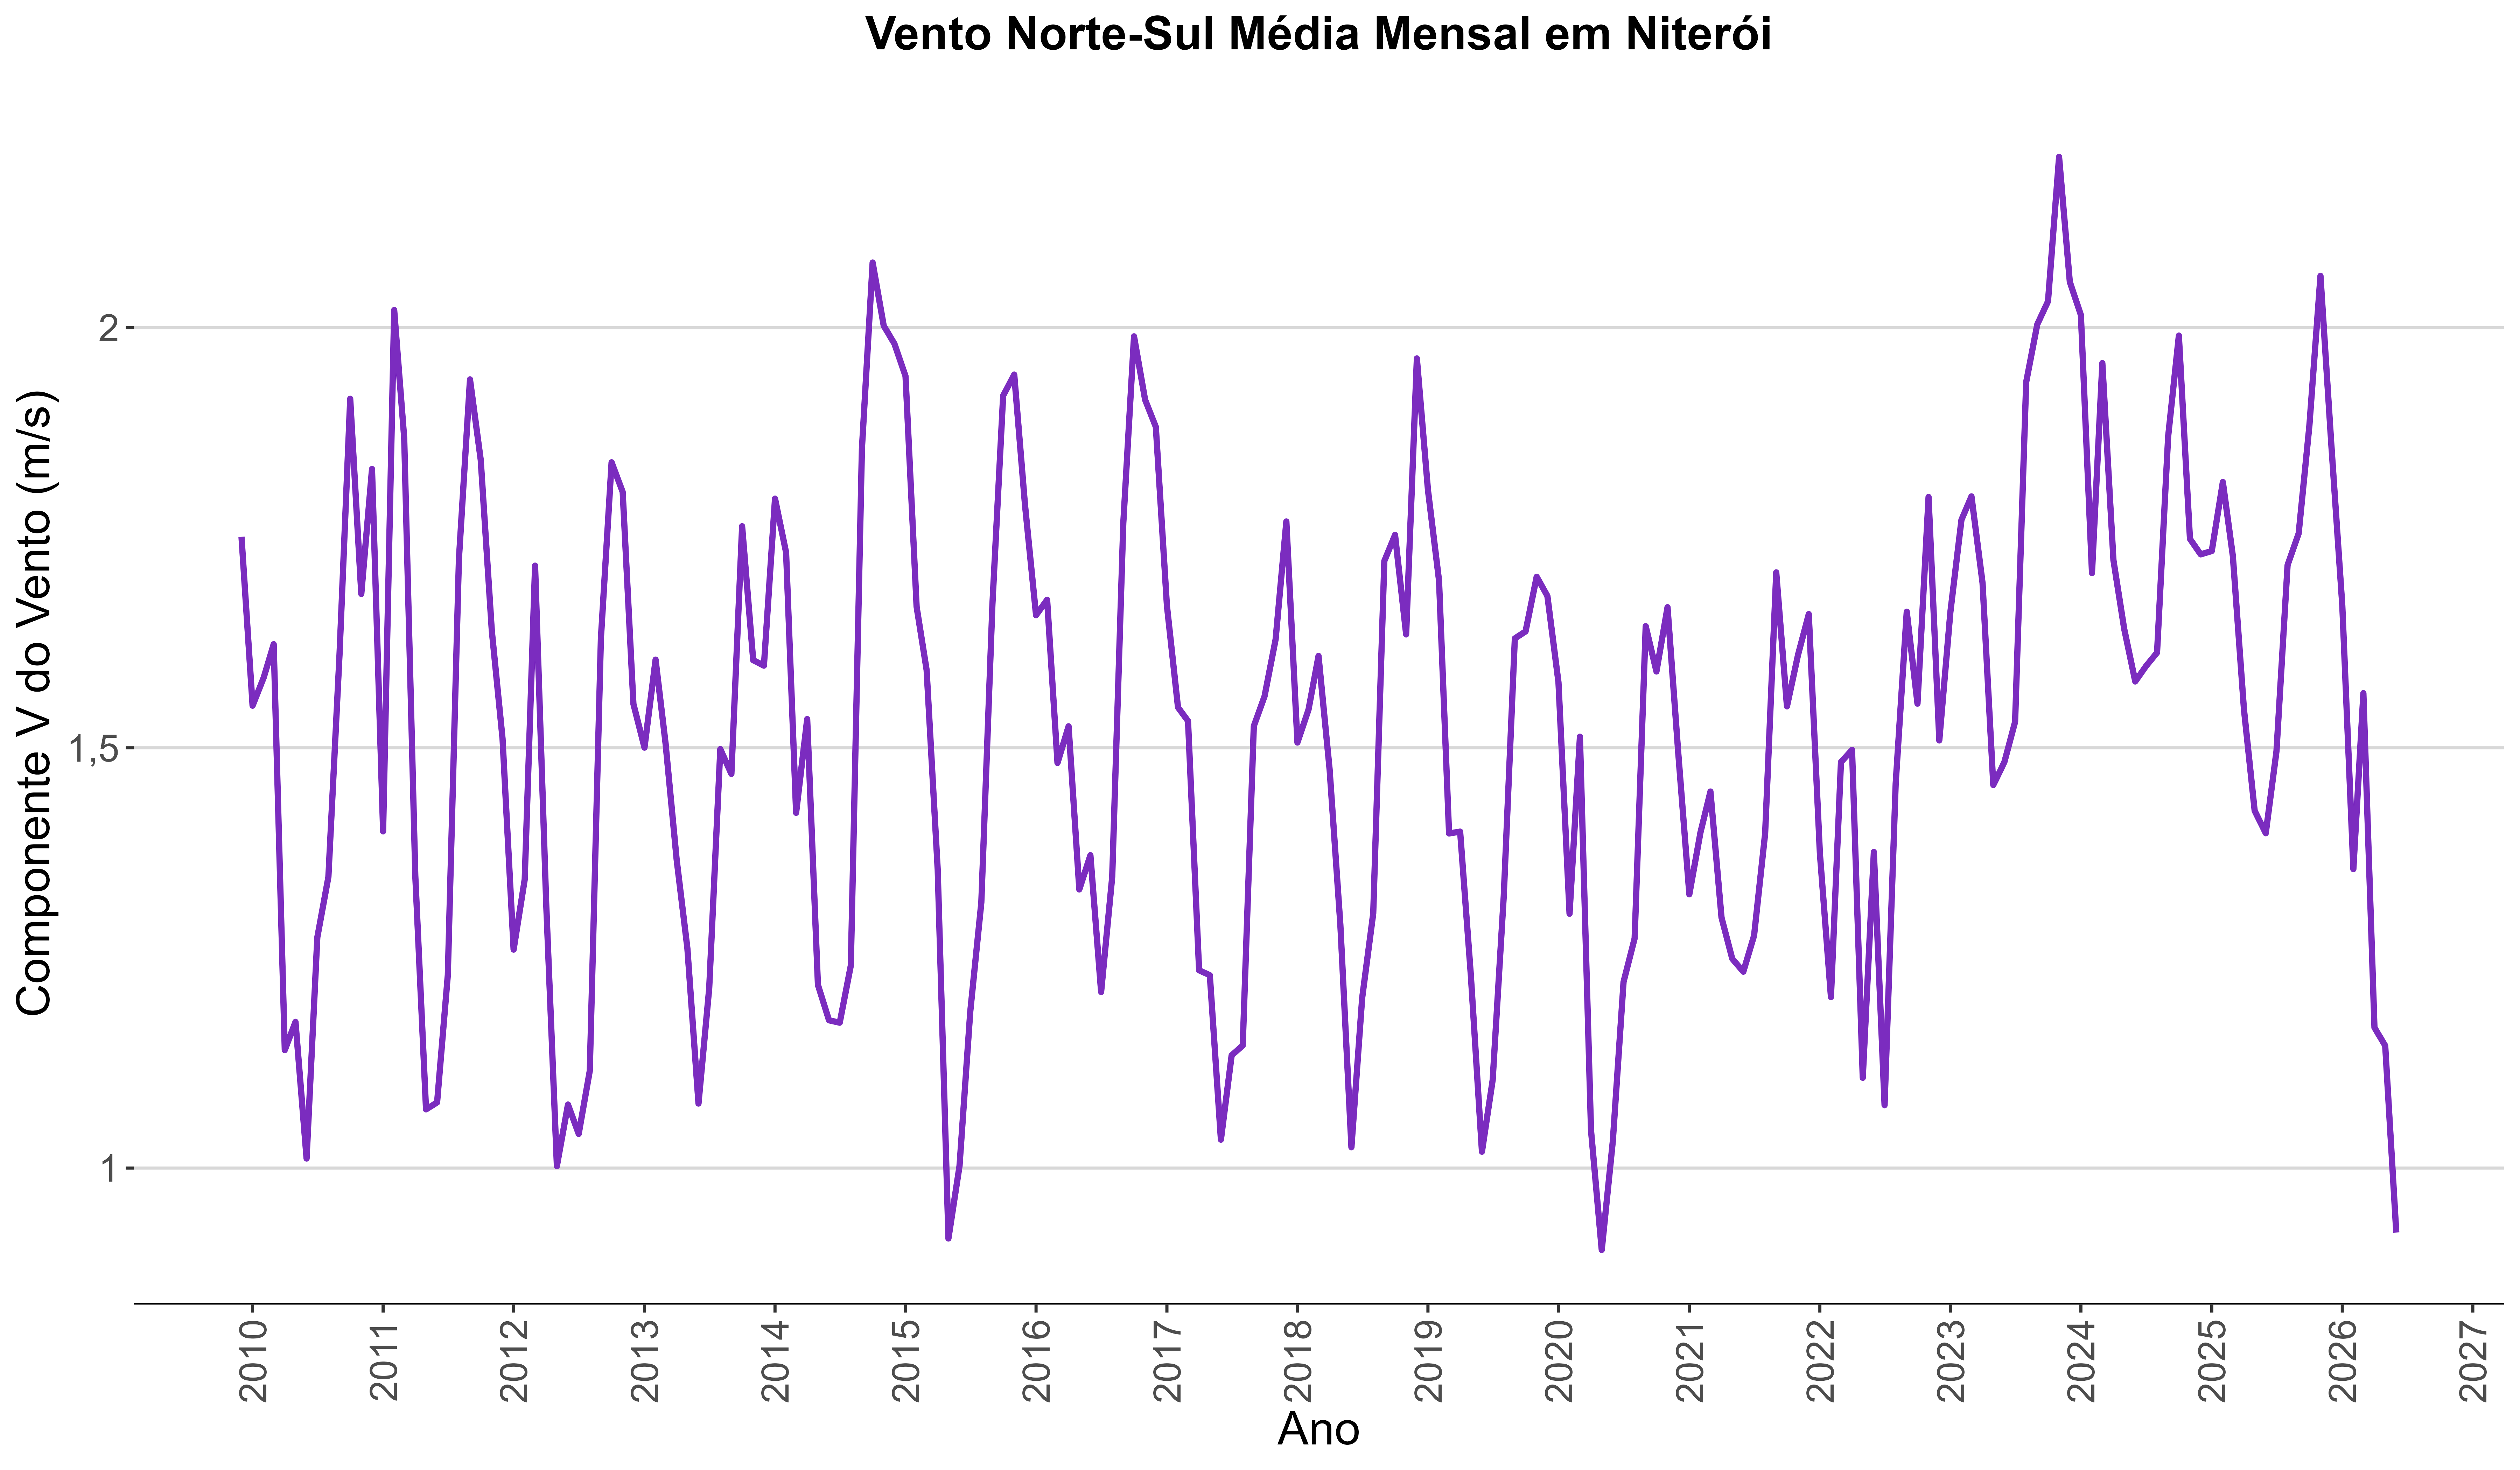
\includegraphics[keepaspectratio]{resultados/VentoV/03_ventov_mensal.png}}

}

\caption{Vento Norte-Sul Médio Mensal}

\end{figure}%

\begin{figure}[H]

{\centering \pandocbounded{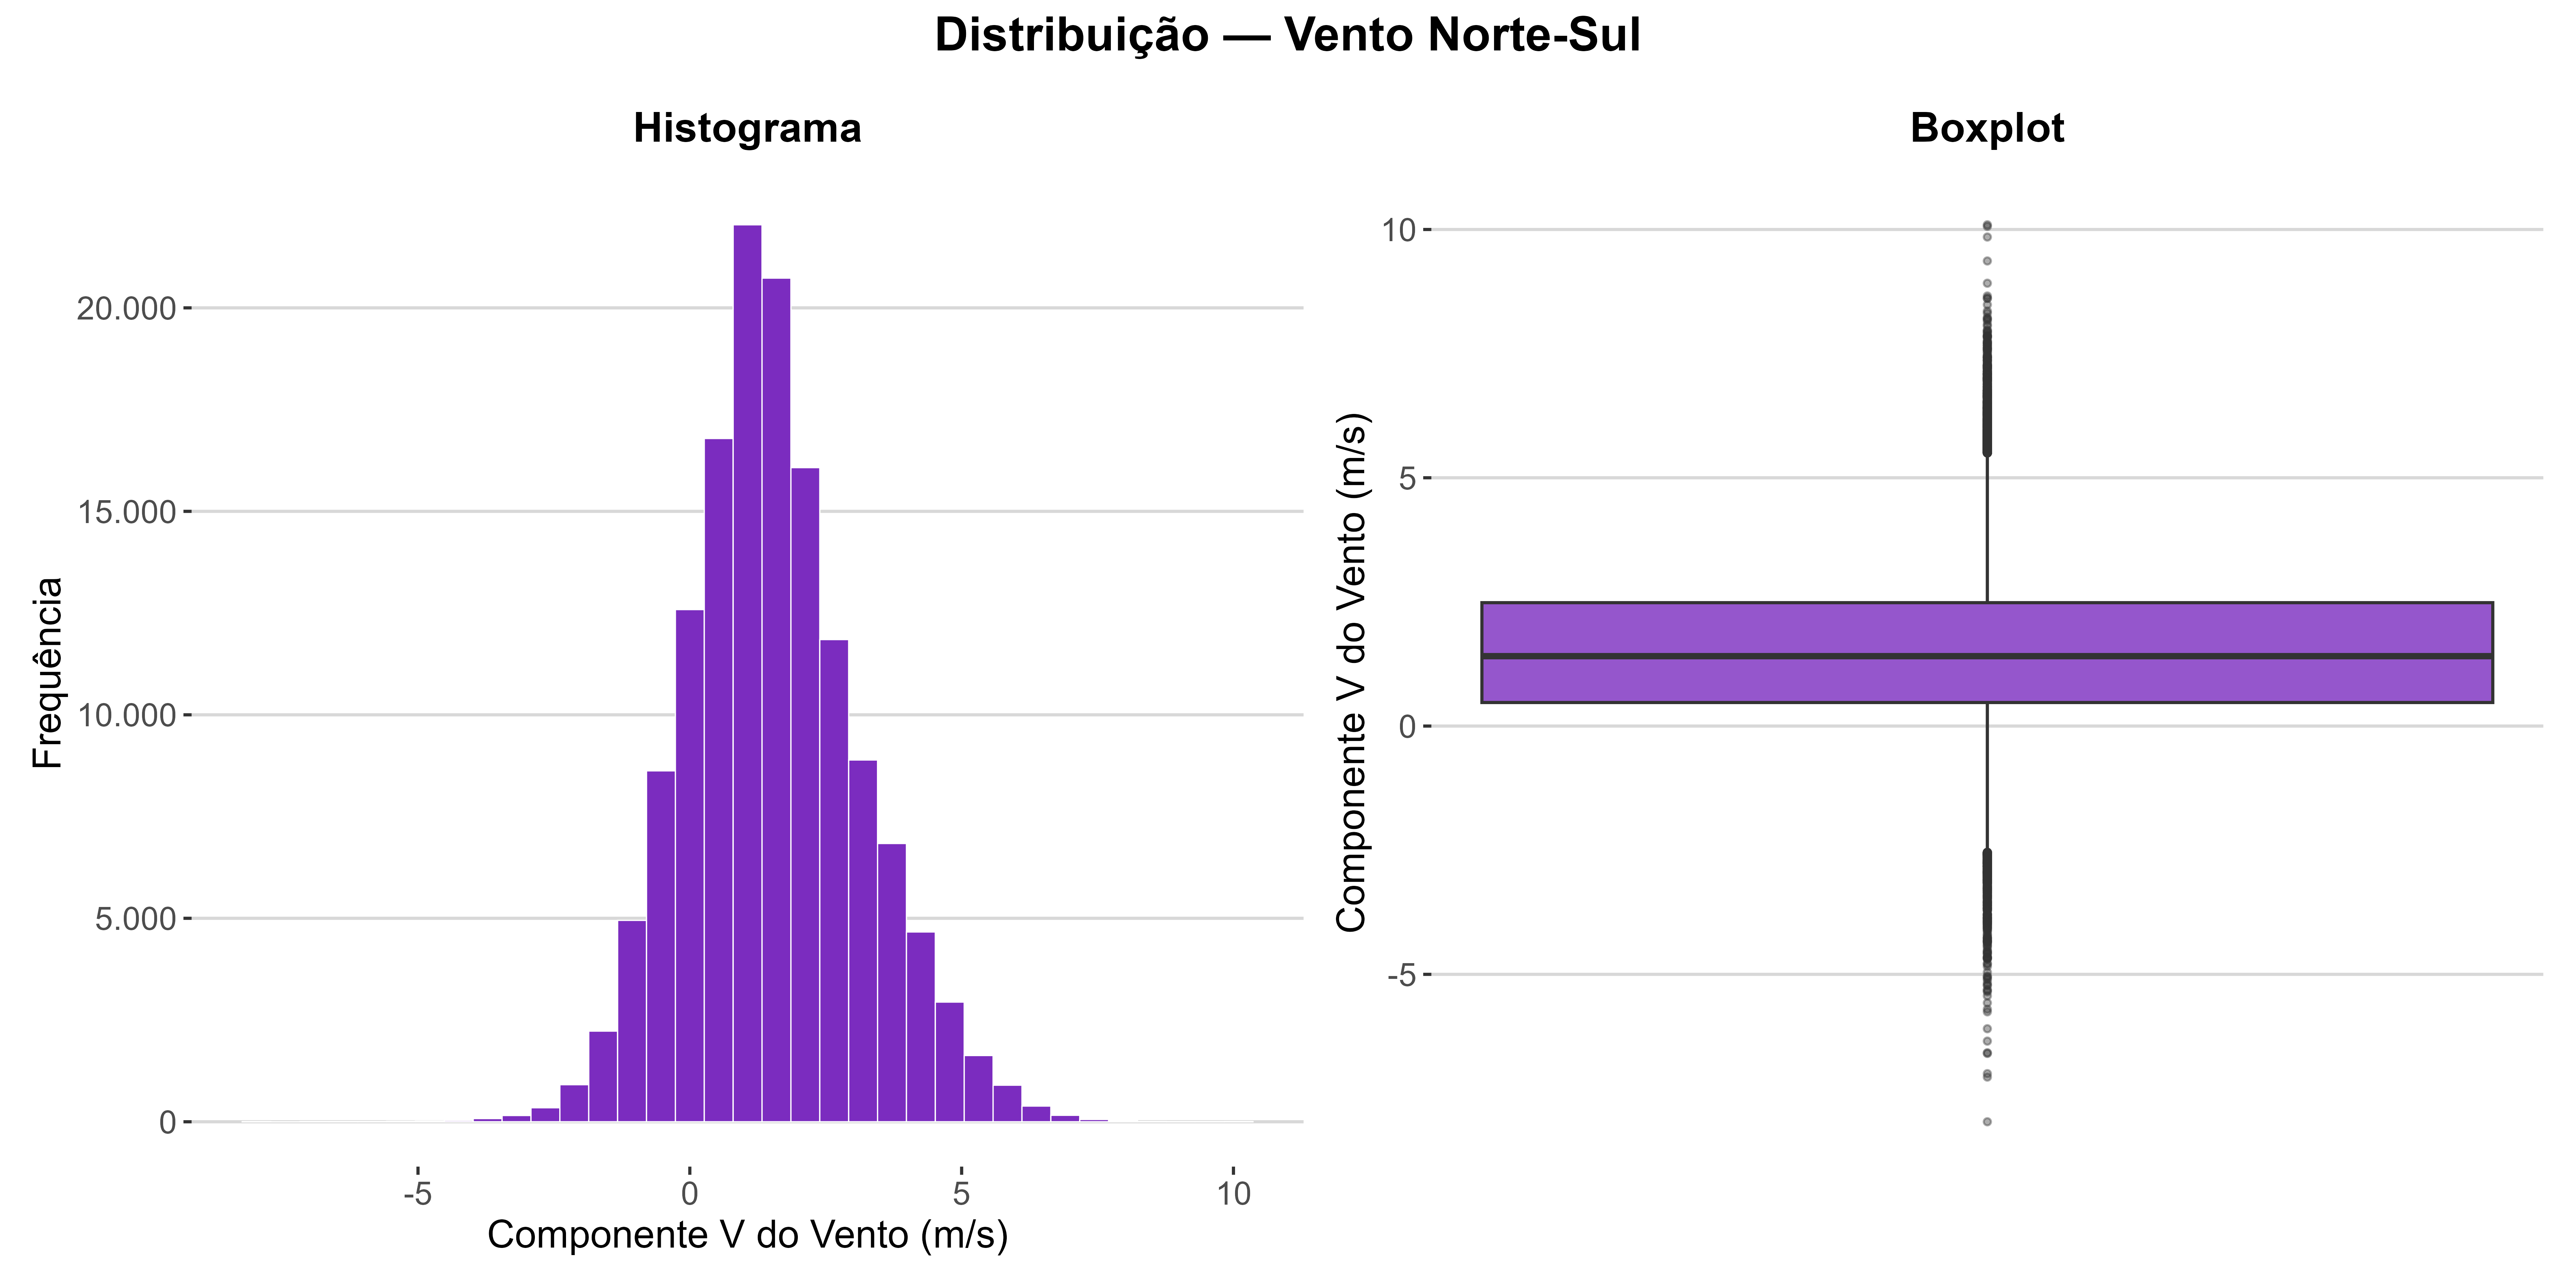
\includegraphics[keepaspectratio]{resultados/VentoV/04_ventov_distribuicao.png}}

}

\caption{Distribuição do Vento Norte-Sul}

\end{figure}%

\paragraph{Principais Achados}\label{principais-achados-11}

A componente V do vento também oscila em torno de zero, com
comportamento mais \textbf{irregular e ruidoso} do que a componente U.

A distribuição é aproximadamente simétrica, ligeiramente mais estreita
do que a componente U. Os dois componentes juntos compõem o campo
vetorial do vento, e sua inclusão no modelo permite capturar a direção
além da intensidade.

\subsubsection{Pressão Superficial}\label{pressuxe3o-superficial}

\begin{figure}[H]

{\centering \pandocbounded{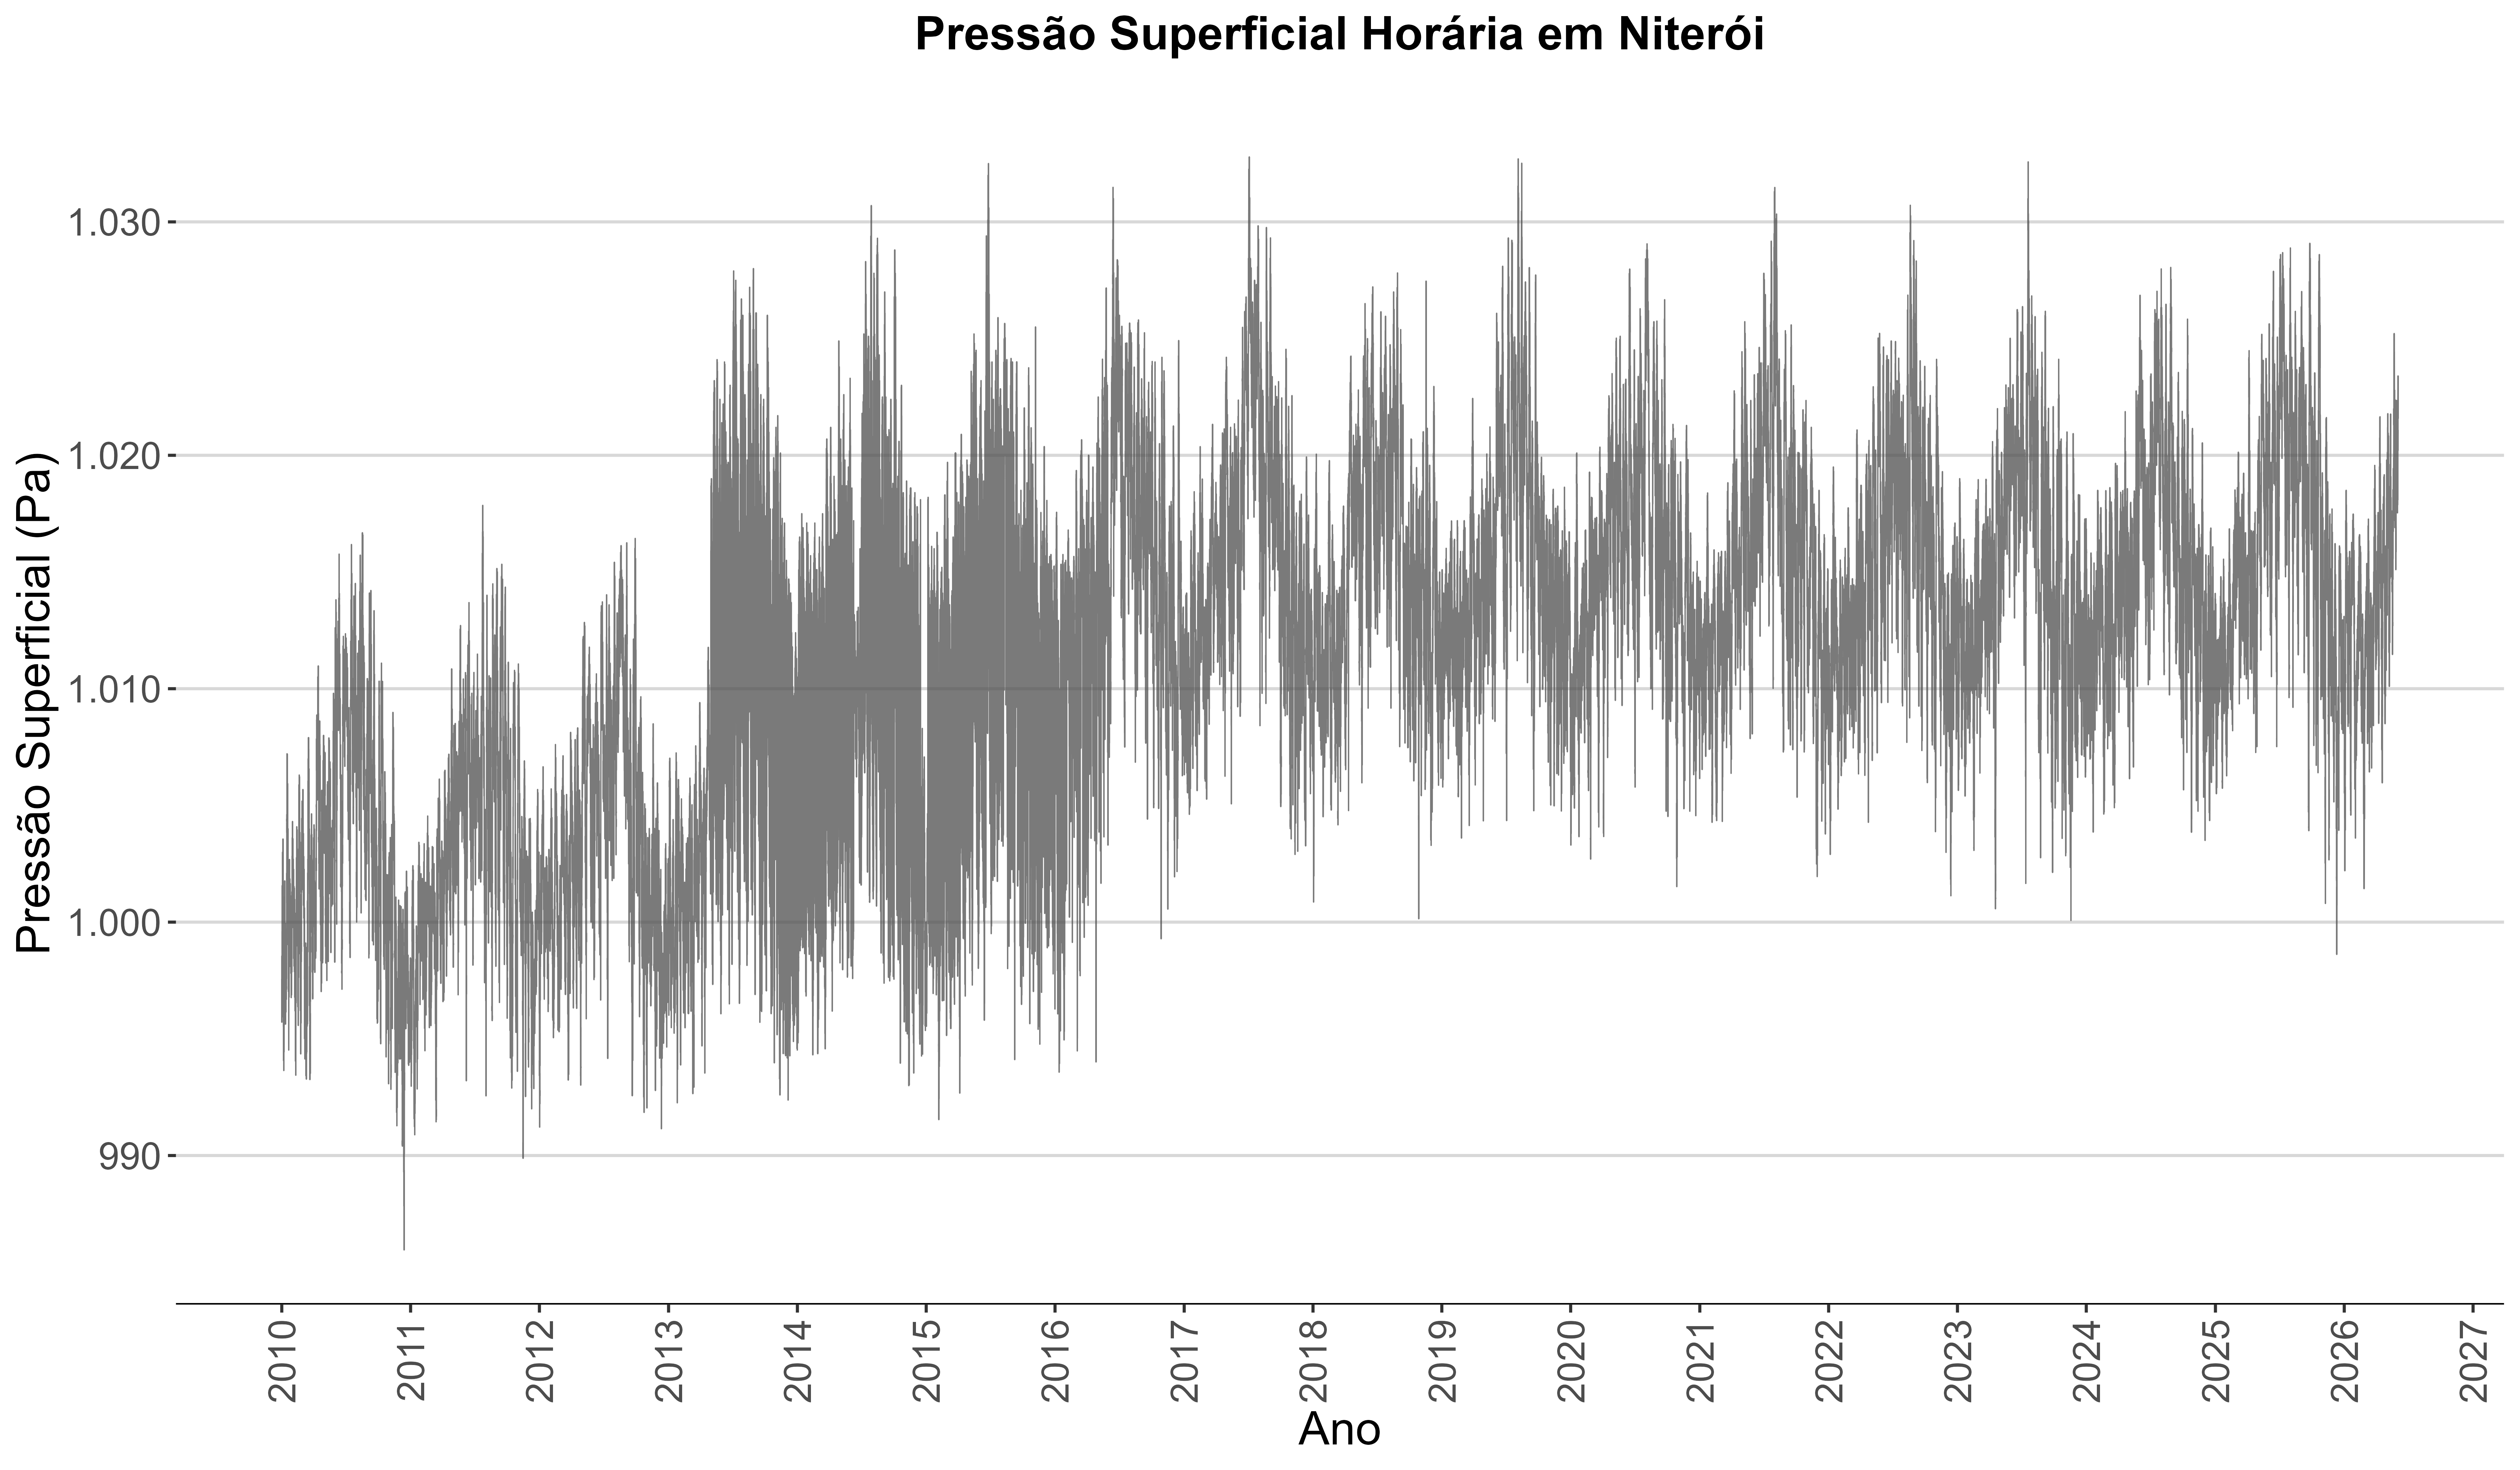
\includegraphics[keepaspectratio]{resultados/Pressao/00_pressao_horario.png}}

}

\caption{Pressão Superficial Horária}

\end{figure}%

\begin{figure}[H]

{\centering \pandocbounded{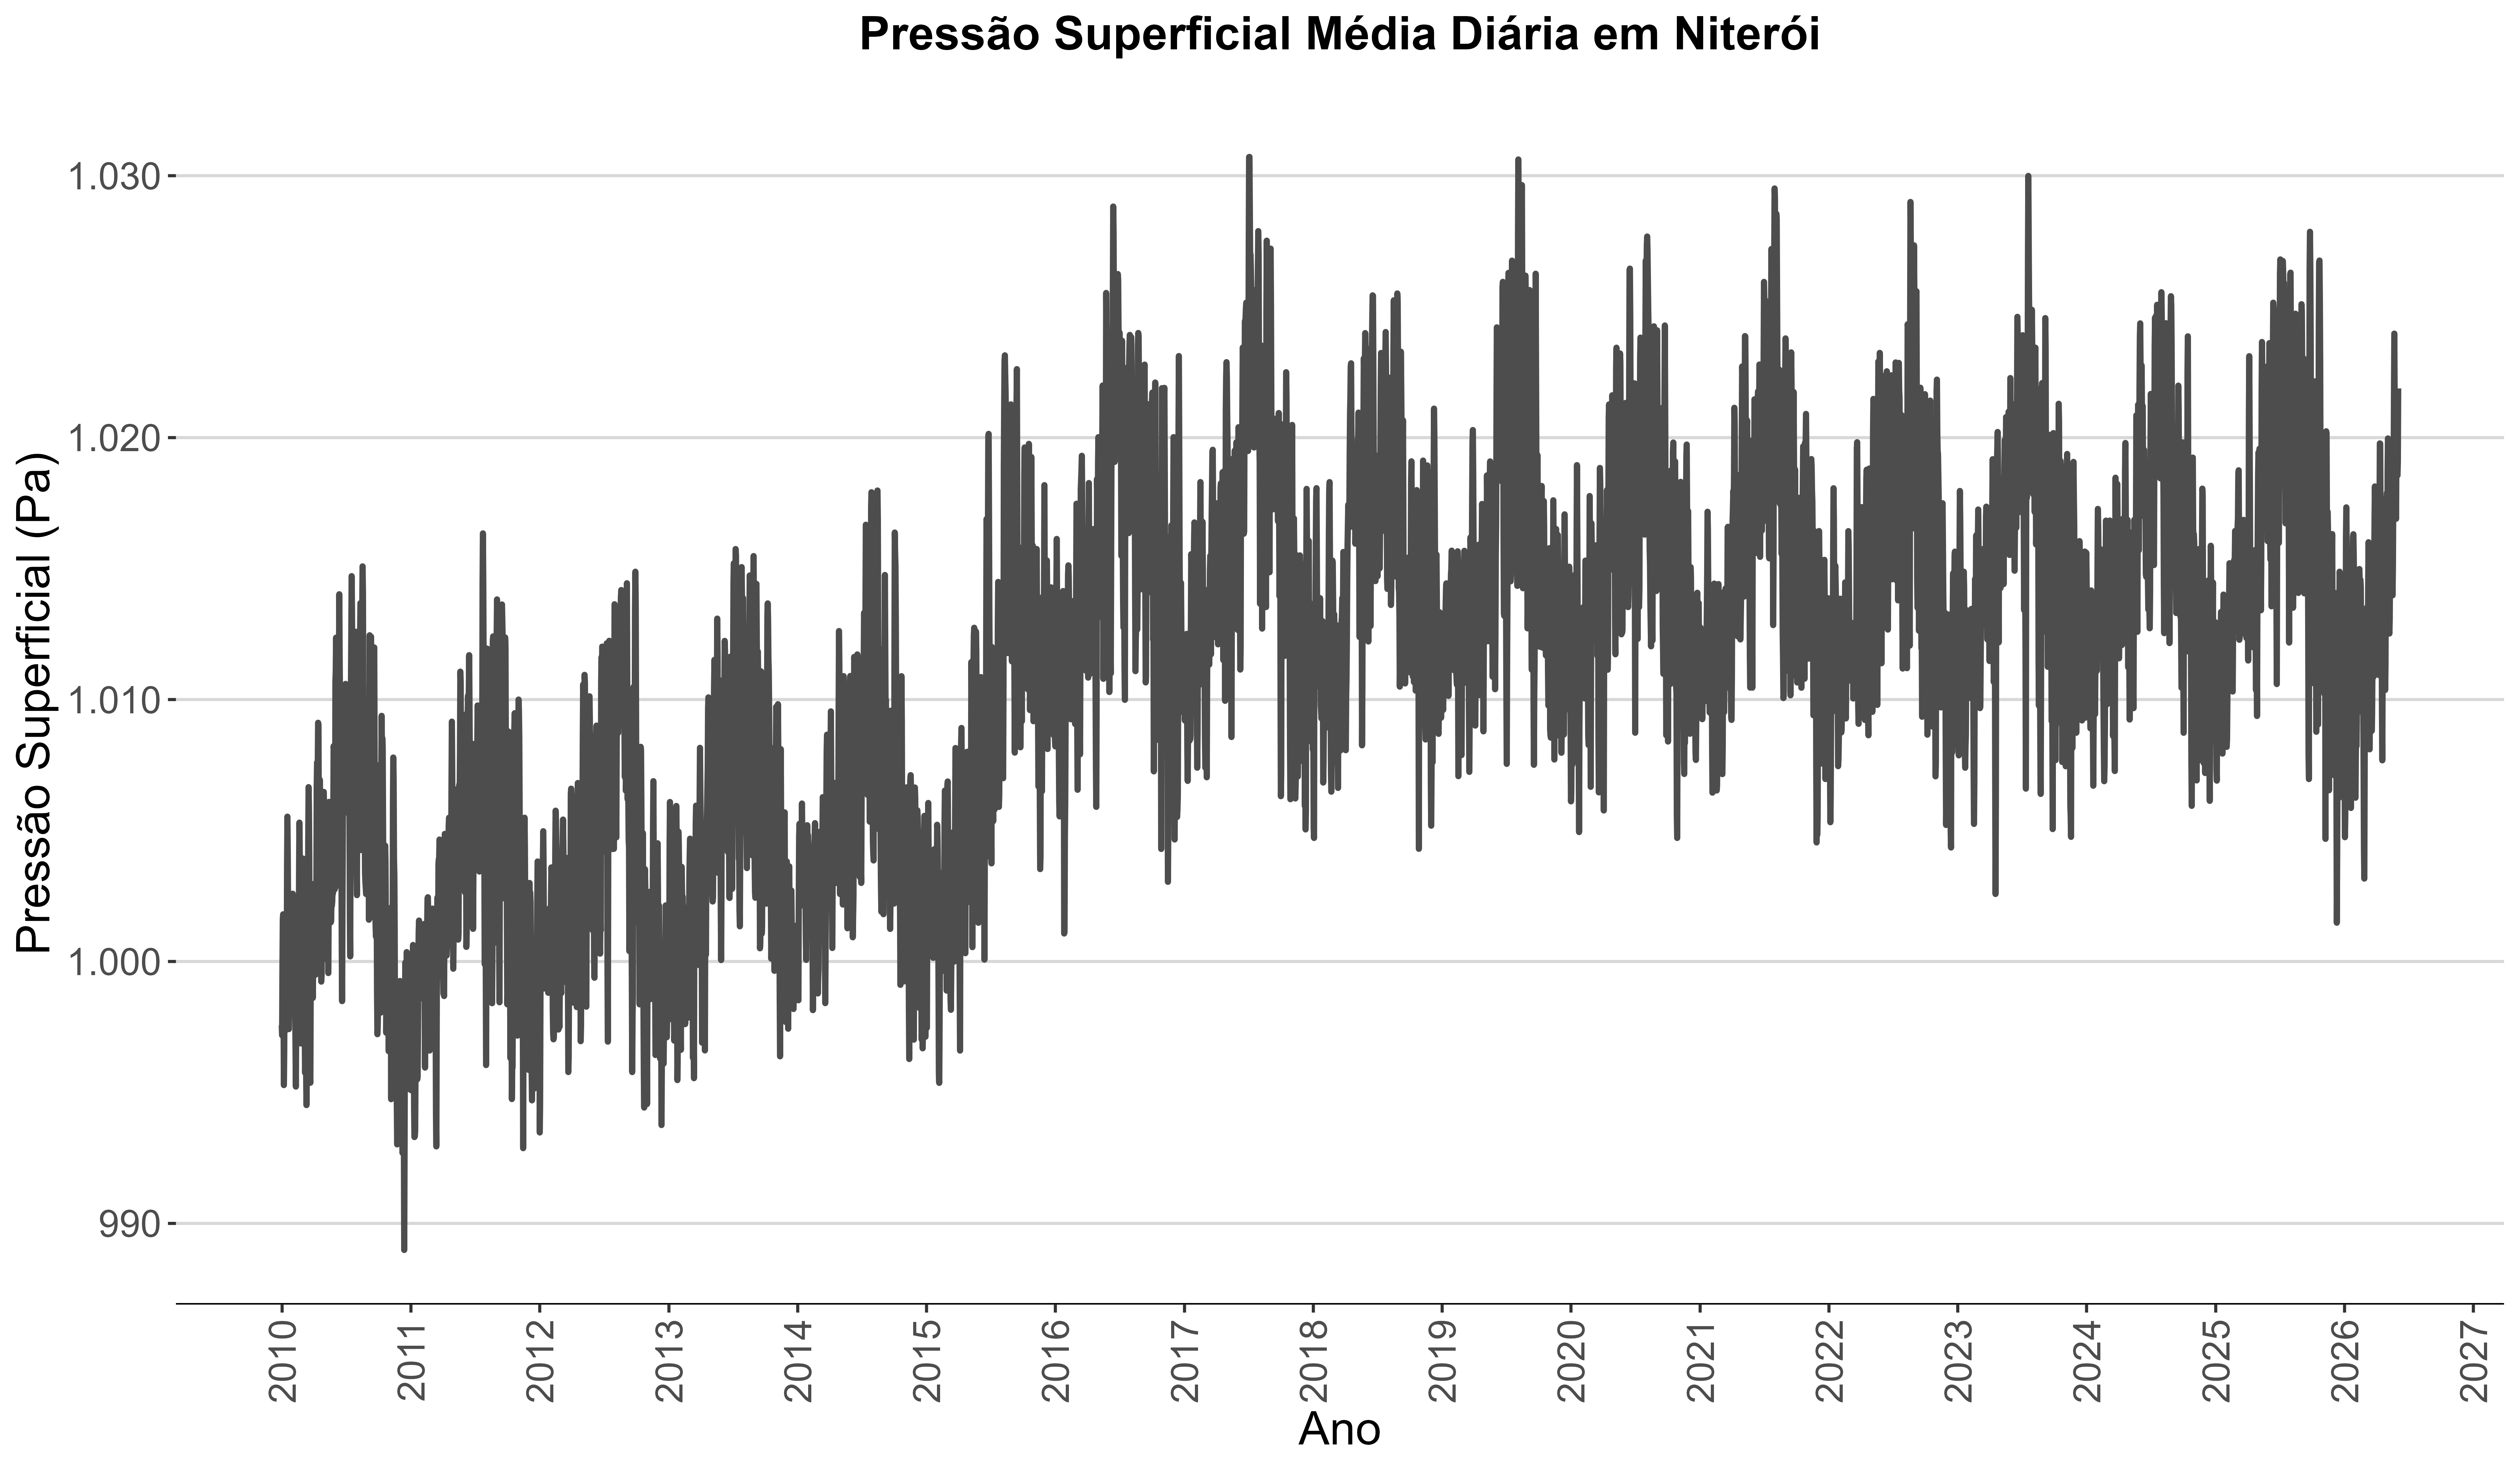
\includegraphics[keepaspectratio]{resultados/Pressao/01_pressao_diario.png}}

}

\caption{Pressão Superficial Média Diária}

\end{figure}%

\begin{figure}[H]

{\centering \pandocbounded{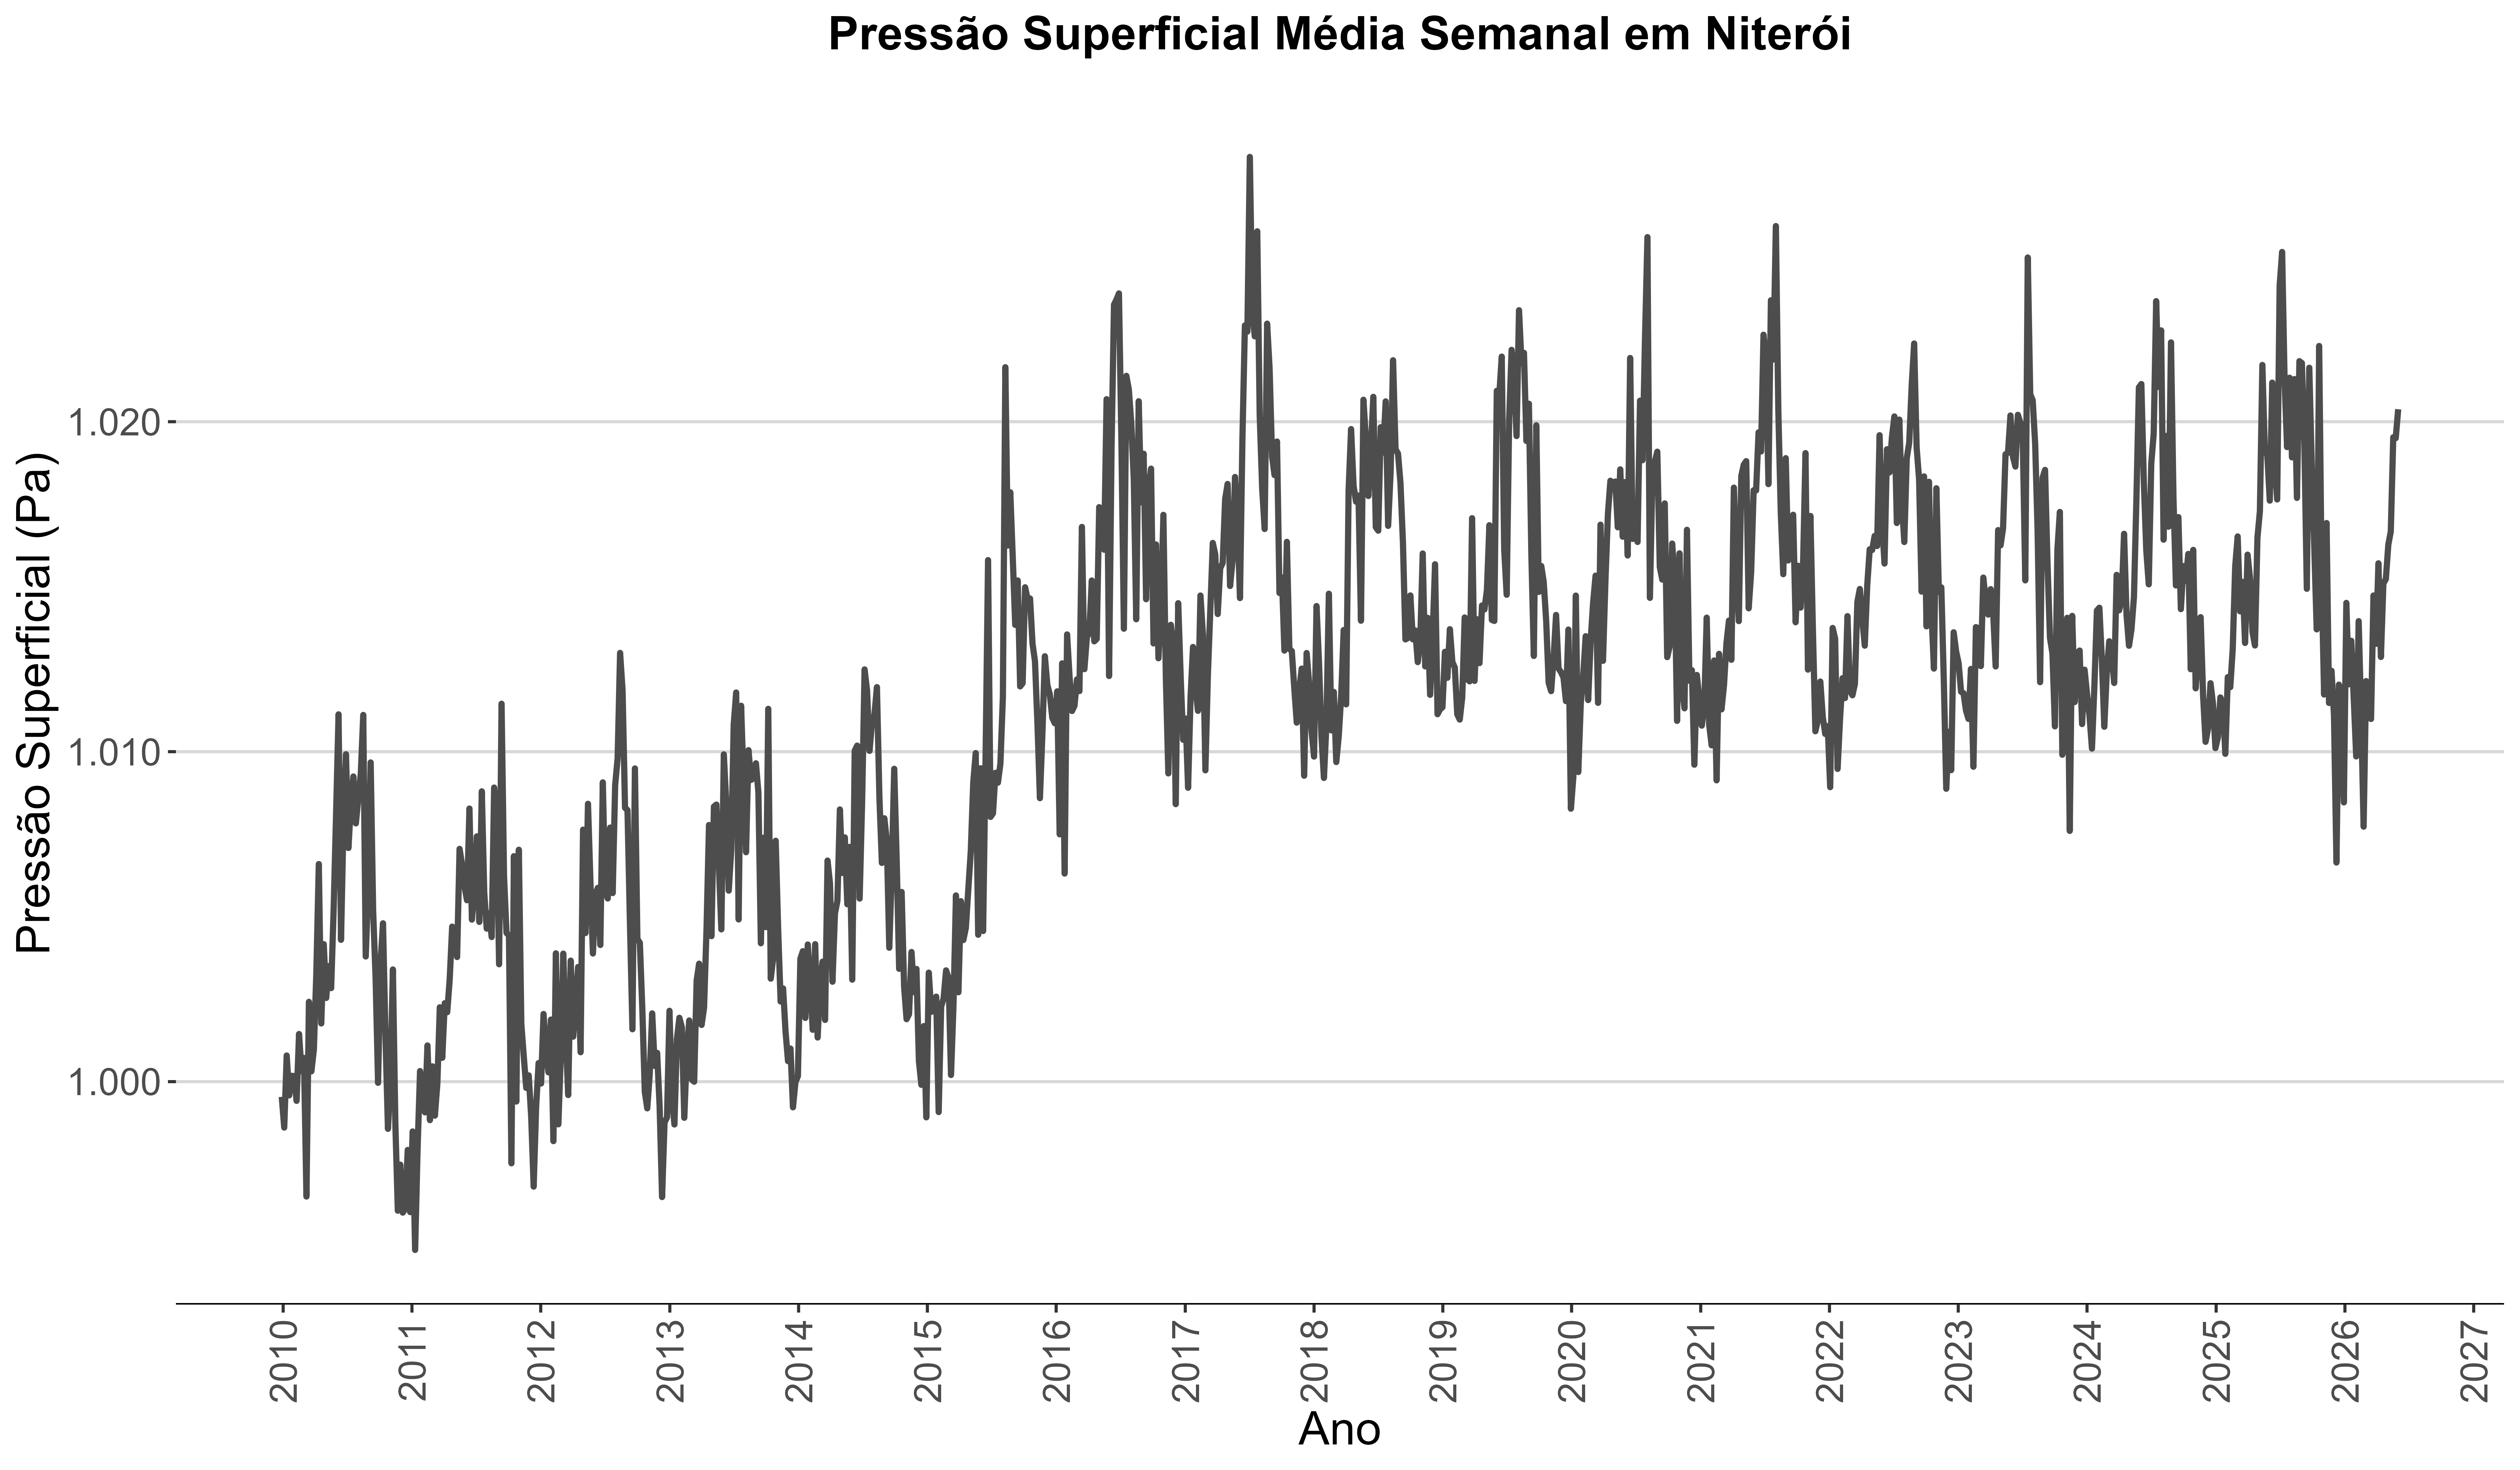
\includegraphics[keepaspectratio]{resultados/Pressao/02_pressao_semanal.png}}

}

\caption{Pressão Superficial Média Semanal}

\end{figure}%

\begin{figure}[H]

{\centering \pandocbounded{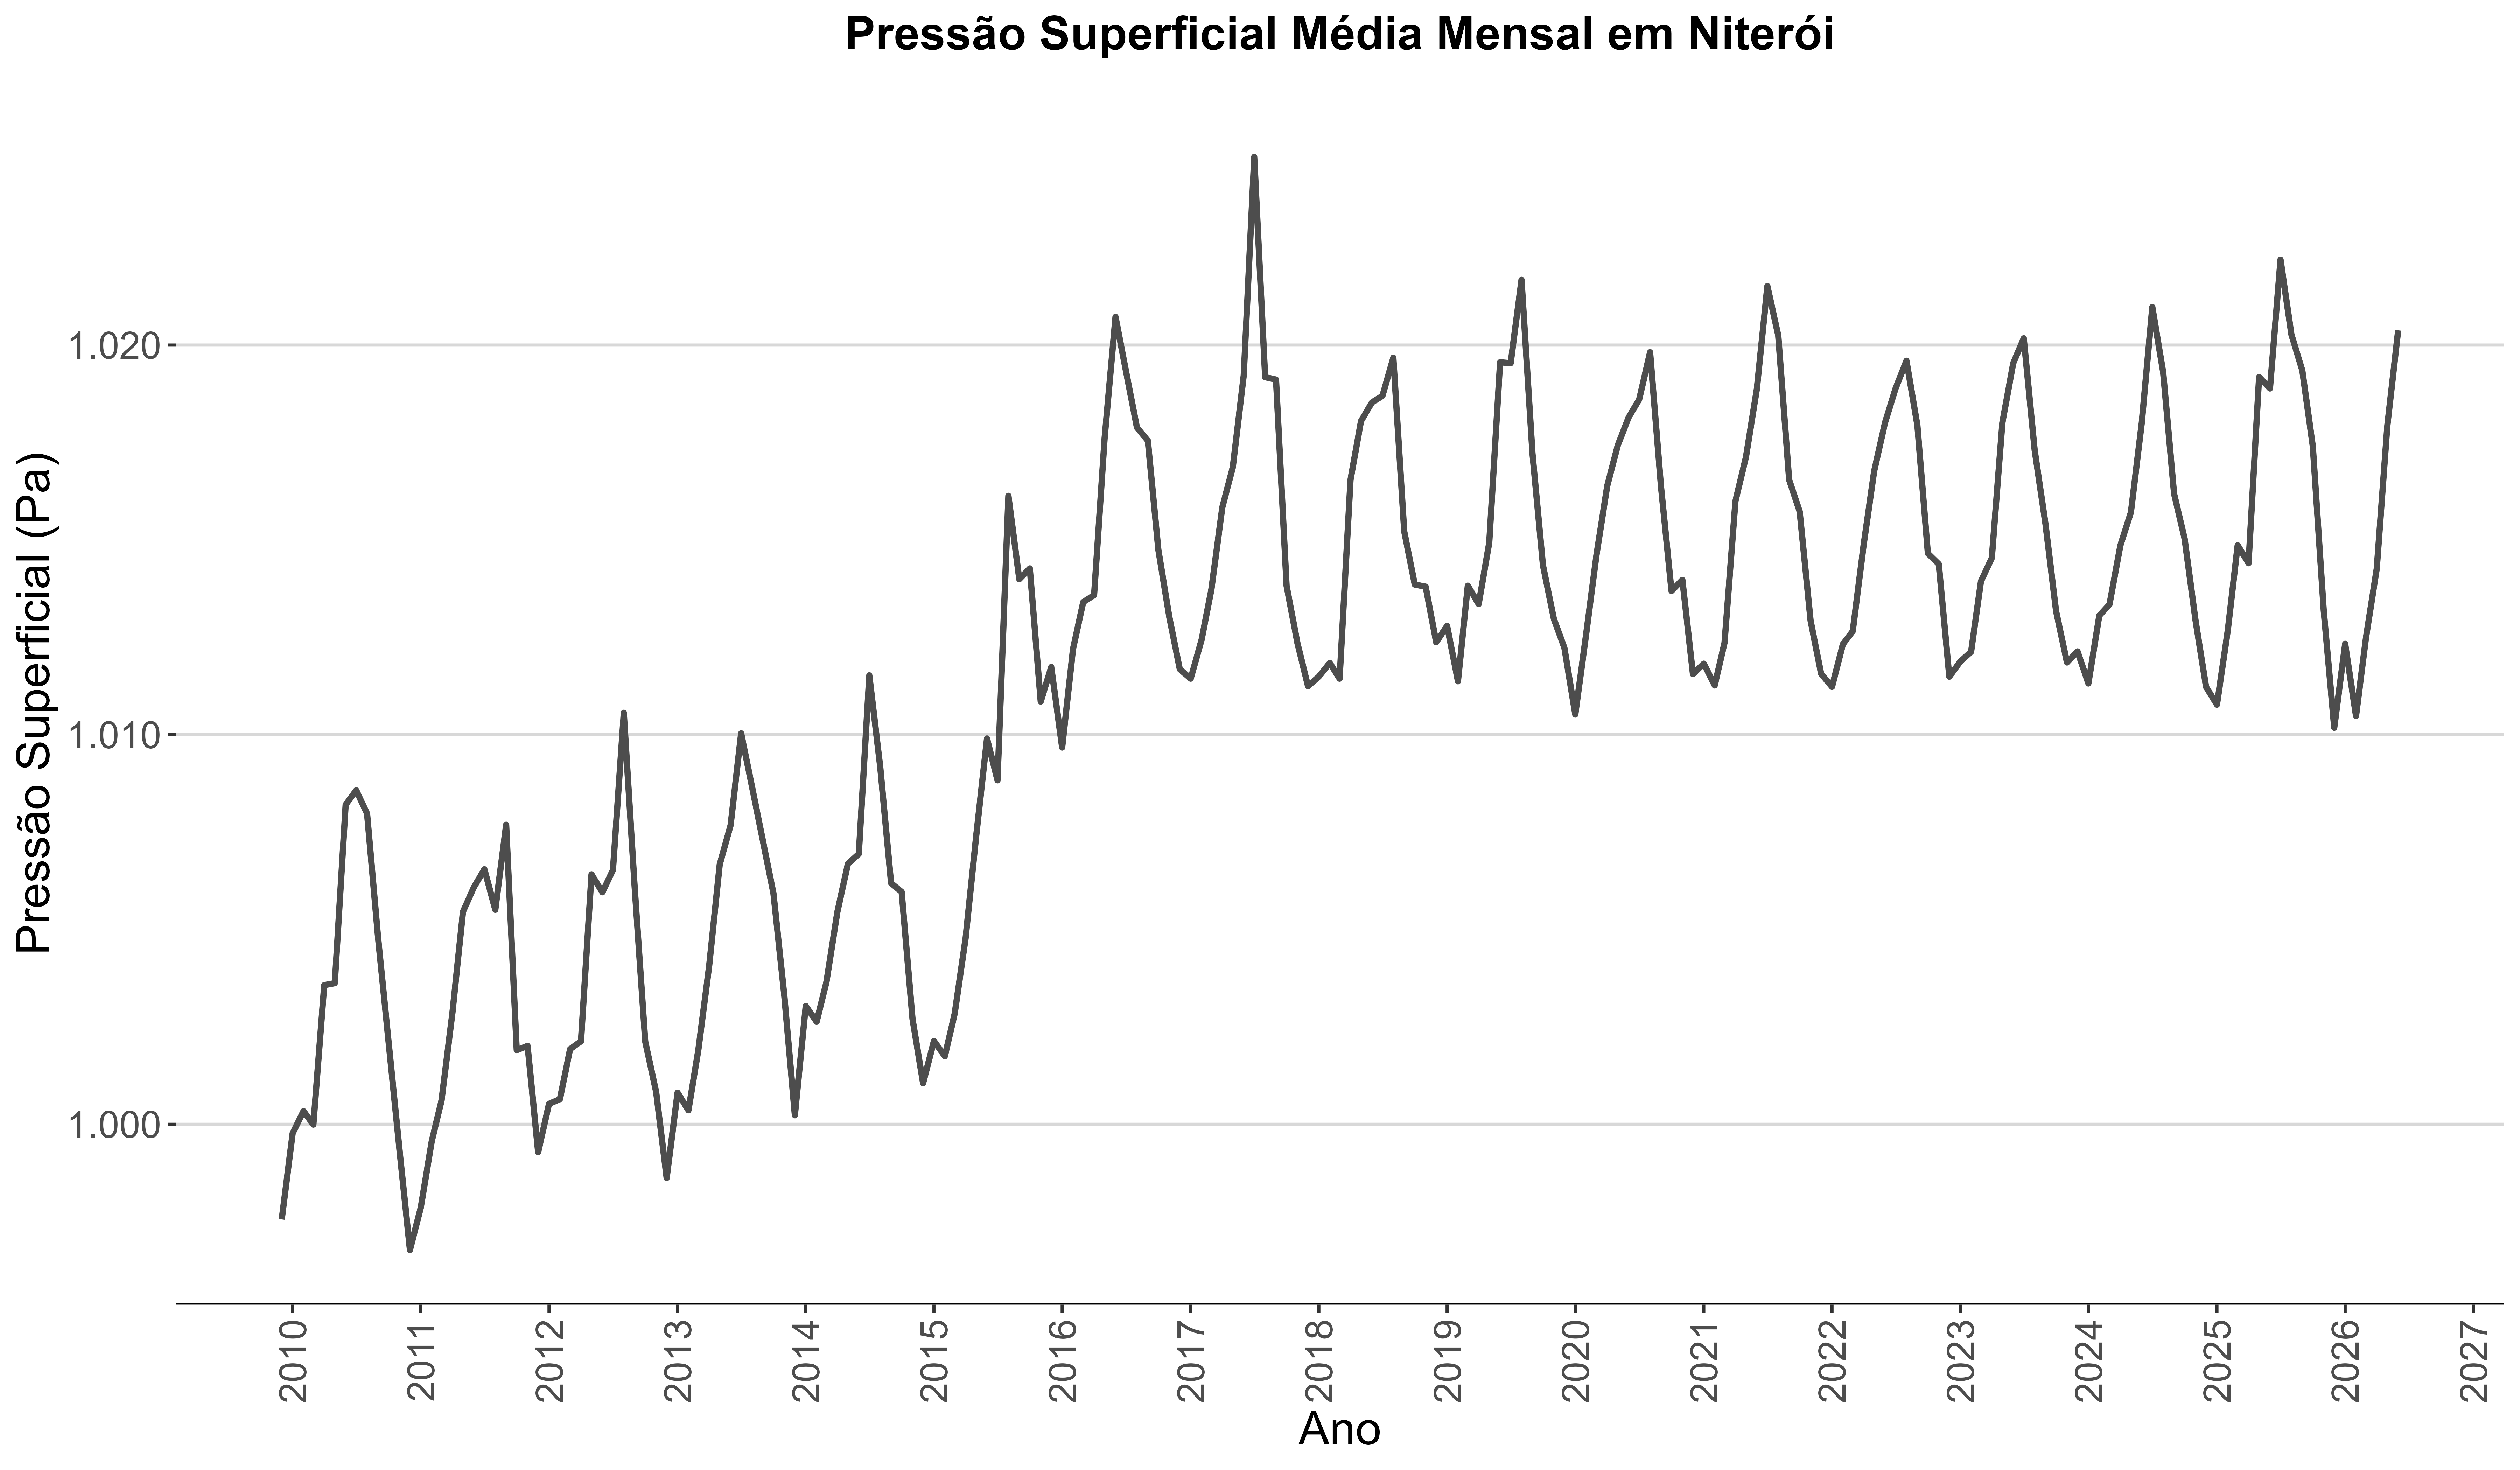
\includegraphics[keepaspectratio]{resultados/Pressao/03_pressao_mensal.png}}

}

\caption{Pressão Superficial Média Mensal}

\end{figure}%

\begin{figure}[H]

{\centering \pandocbounded{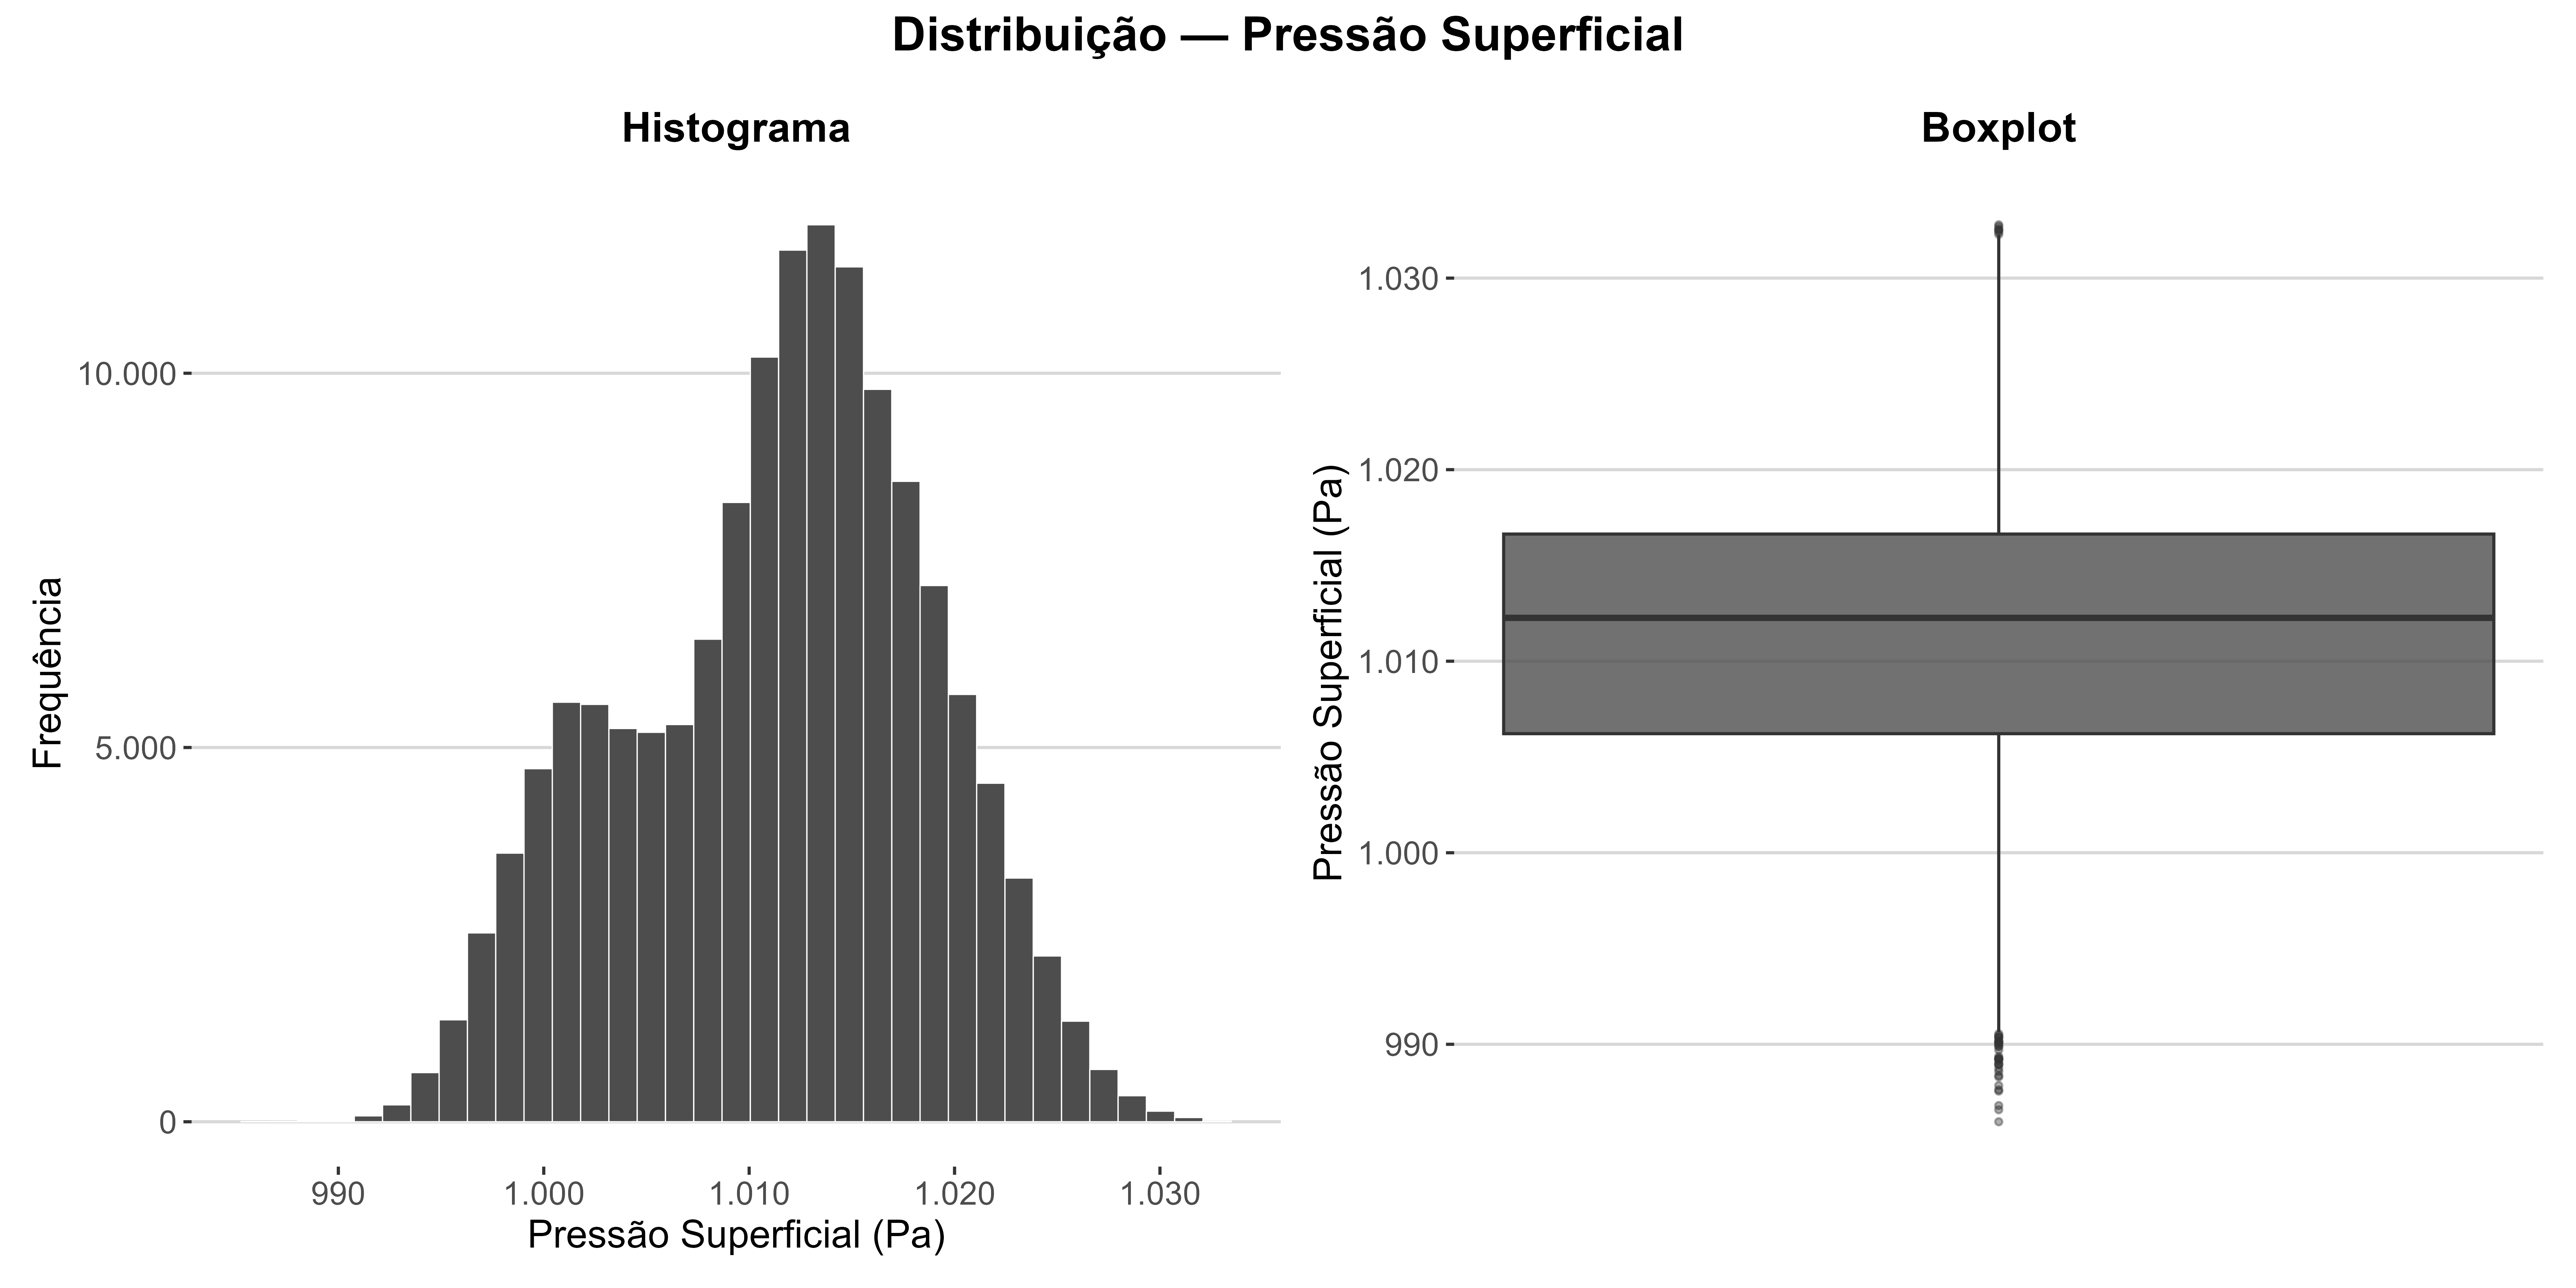
\includegraphics[keepaspectratio]{resultados/Pressao/04_pressao_distribuicao.png}}

}

\caption{Distribuição da Pressão Superficial}

\end{figure}%

\paragraph{Principais Achados}\label{principais-achados-12}

A pressão superficial é a variável de \textbf{menor variabilidade
relativa} de toda a base: os valores mensais oscilam em uma faixa
estreita, de aproximadamente 10 Pa. As séries horárias revelam um ciclo
de maré barométrica de \textasciitilde12 horas (duas oscilações por
dia), enquanto as variações de menor frequência refletem a passagem de
sistemas sinóticos (frentes frias e anticiclones). Resalta-se uma
translação da série em 10 Pa a partir do ano de 2016

A distribuição é a mais simétrica e bimodal. A baixa amplitude e a
previsibilidade do ciclo diário tornam essa variável potencialmente útil
como âncora temporal para o modelo LSTM.

\section{Análises Conjuntas}\label{anuxe1lises-conjuntas}

\begin{figure}[H]

{\centering \pandocbounded{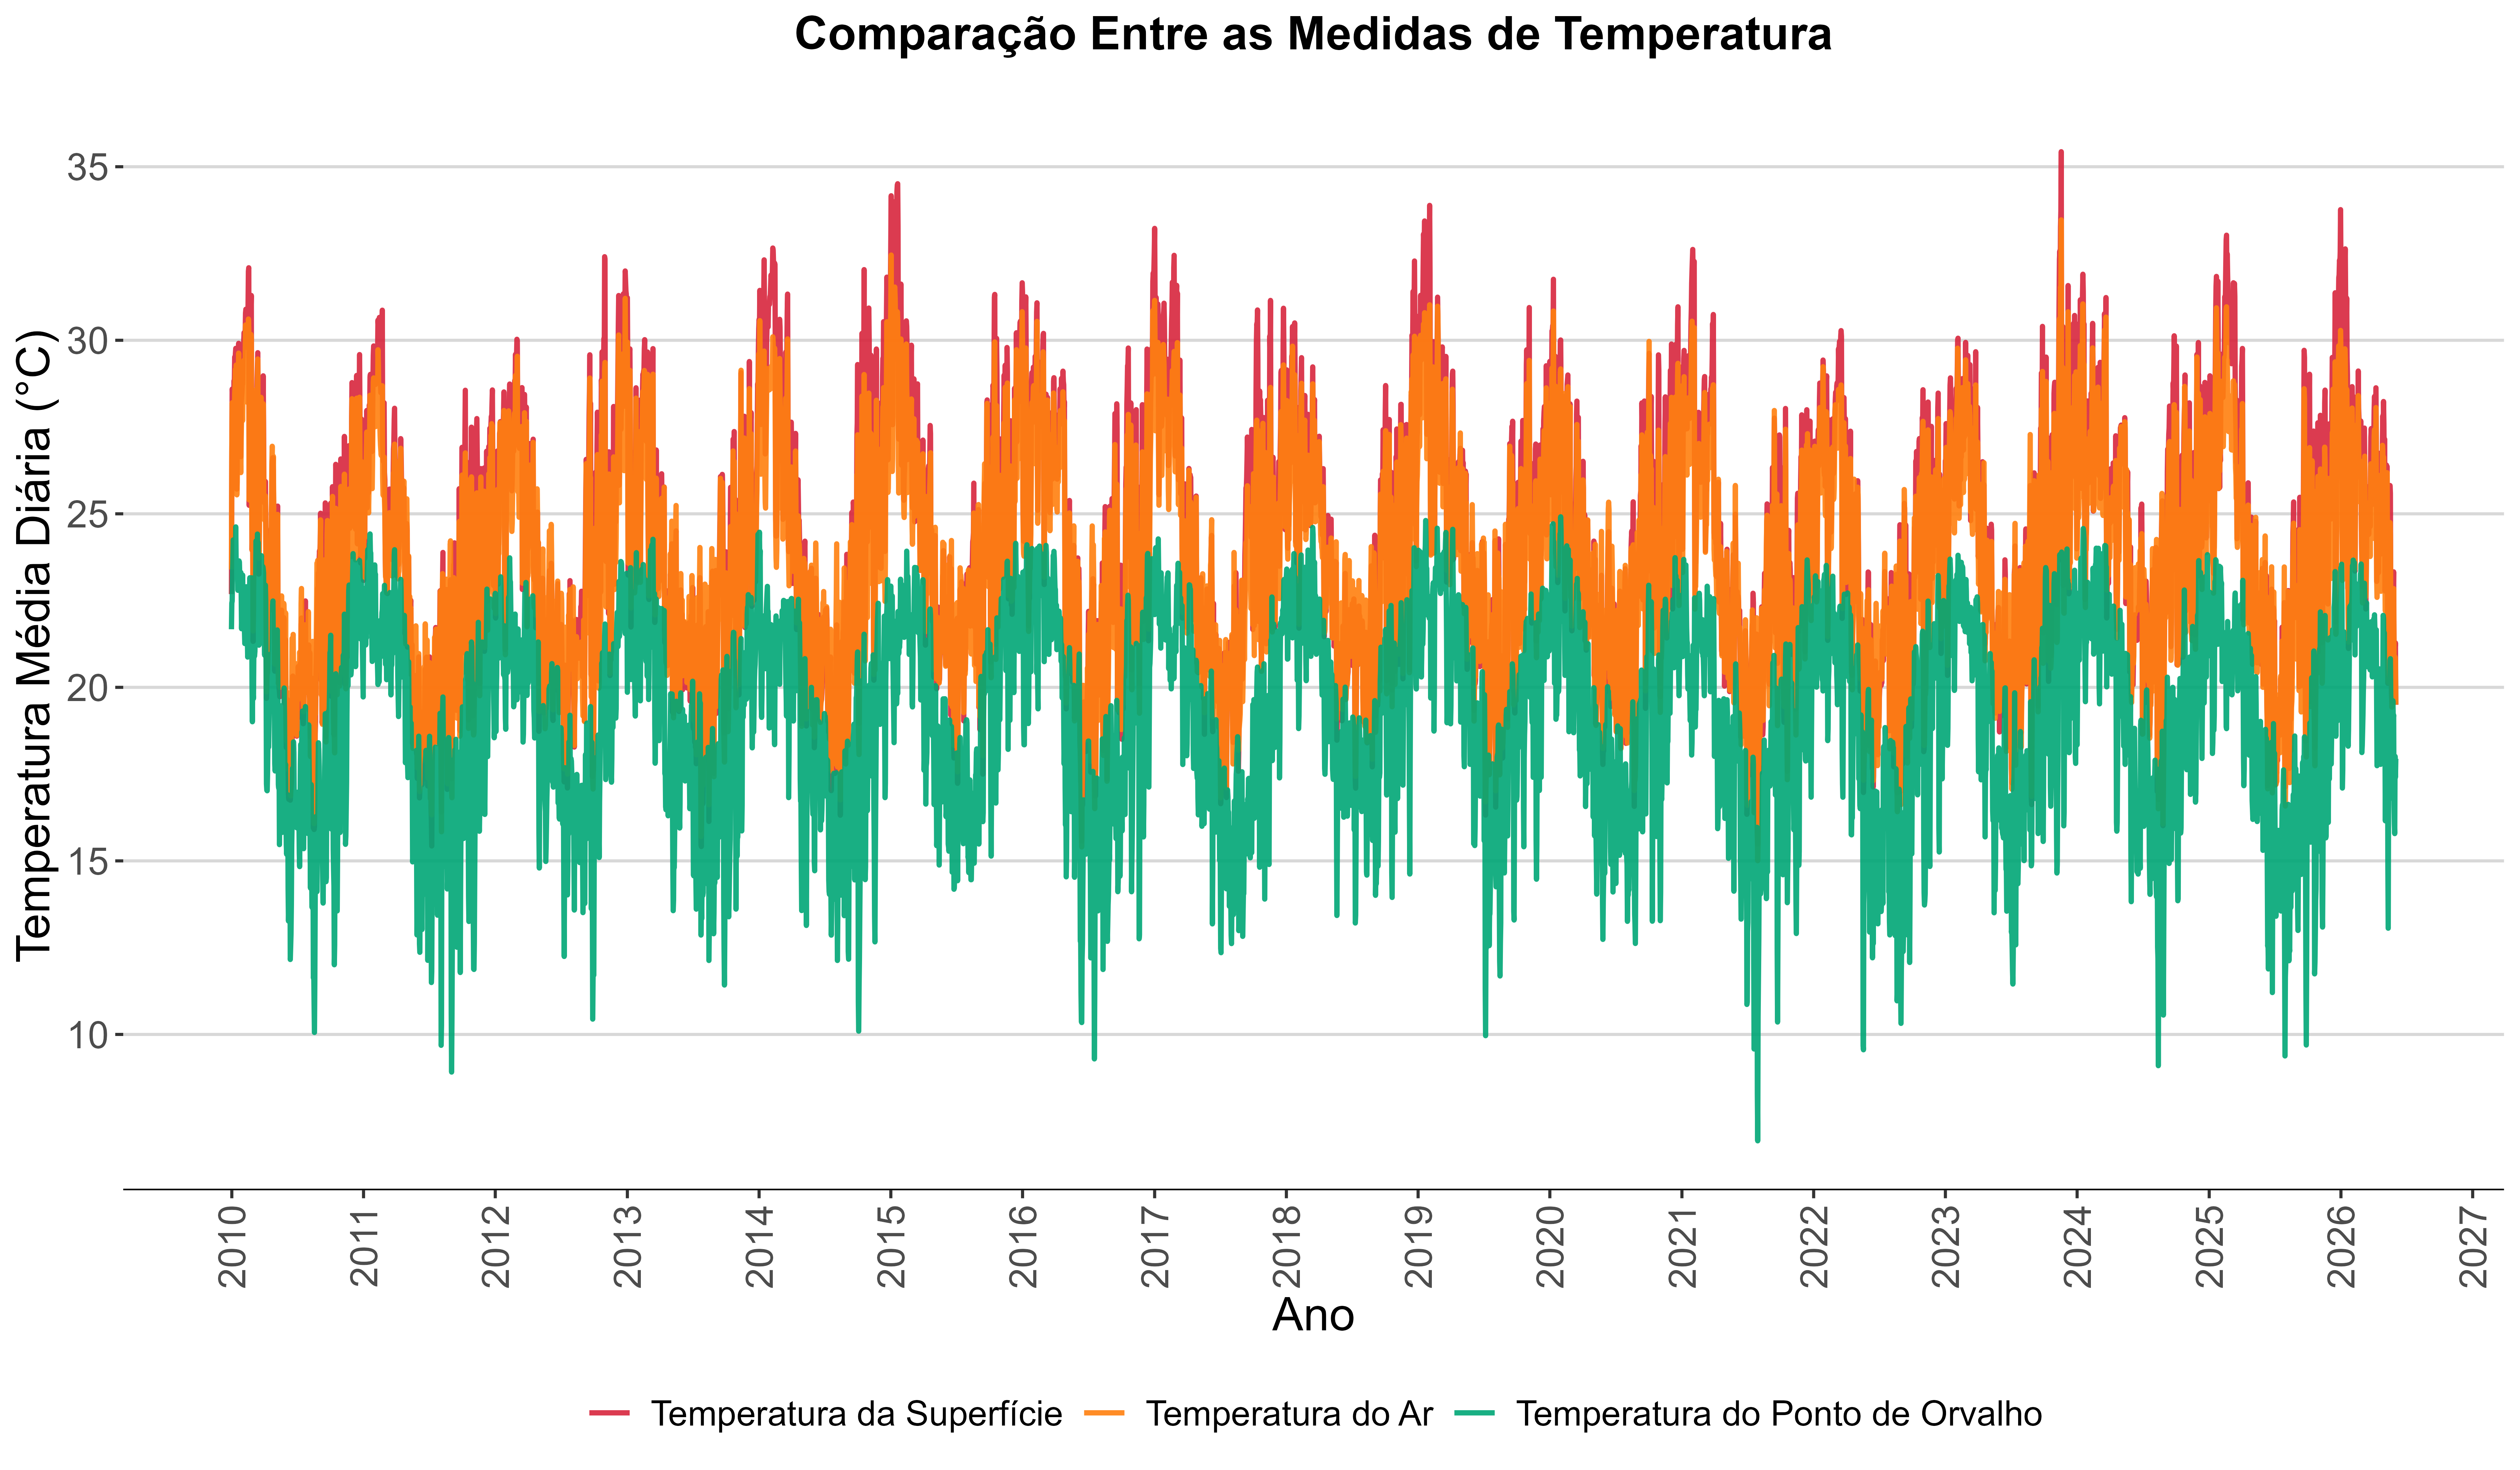
\includegraphics[keepaspectratio]{resultados/30_series_sobrepostas_temperaturas.png}}

}

\caption{Comparação Entre as Medidas de Temperatura}

\end{figure}%

\begin{quote}
\textbf{Comentário:} Este gráfico demonstra a altíssima sincronia entre
as três medidas. A temperatura da superfície atinge os picos mais
elevados durante o dia, enquanto a temperatura do ponto de orvalho
permanece consistentemente como o limite inferior, nunca ultrapassando a
temperatura do ar
\end{quote}

\begin{figure}[H]

{\centering \pandocbounded{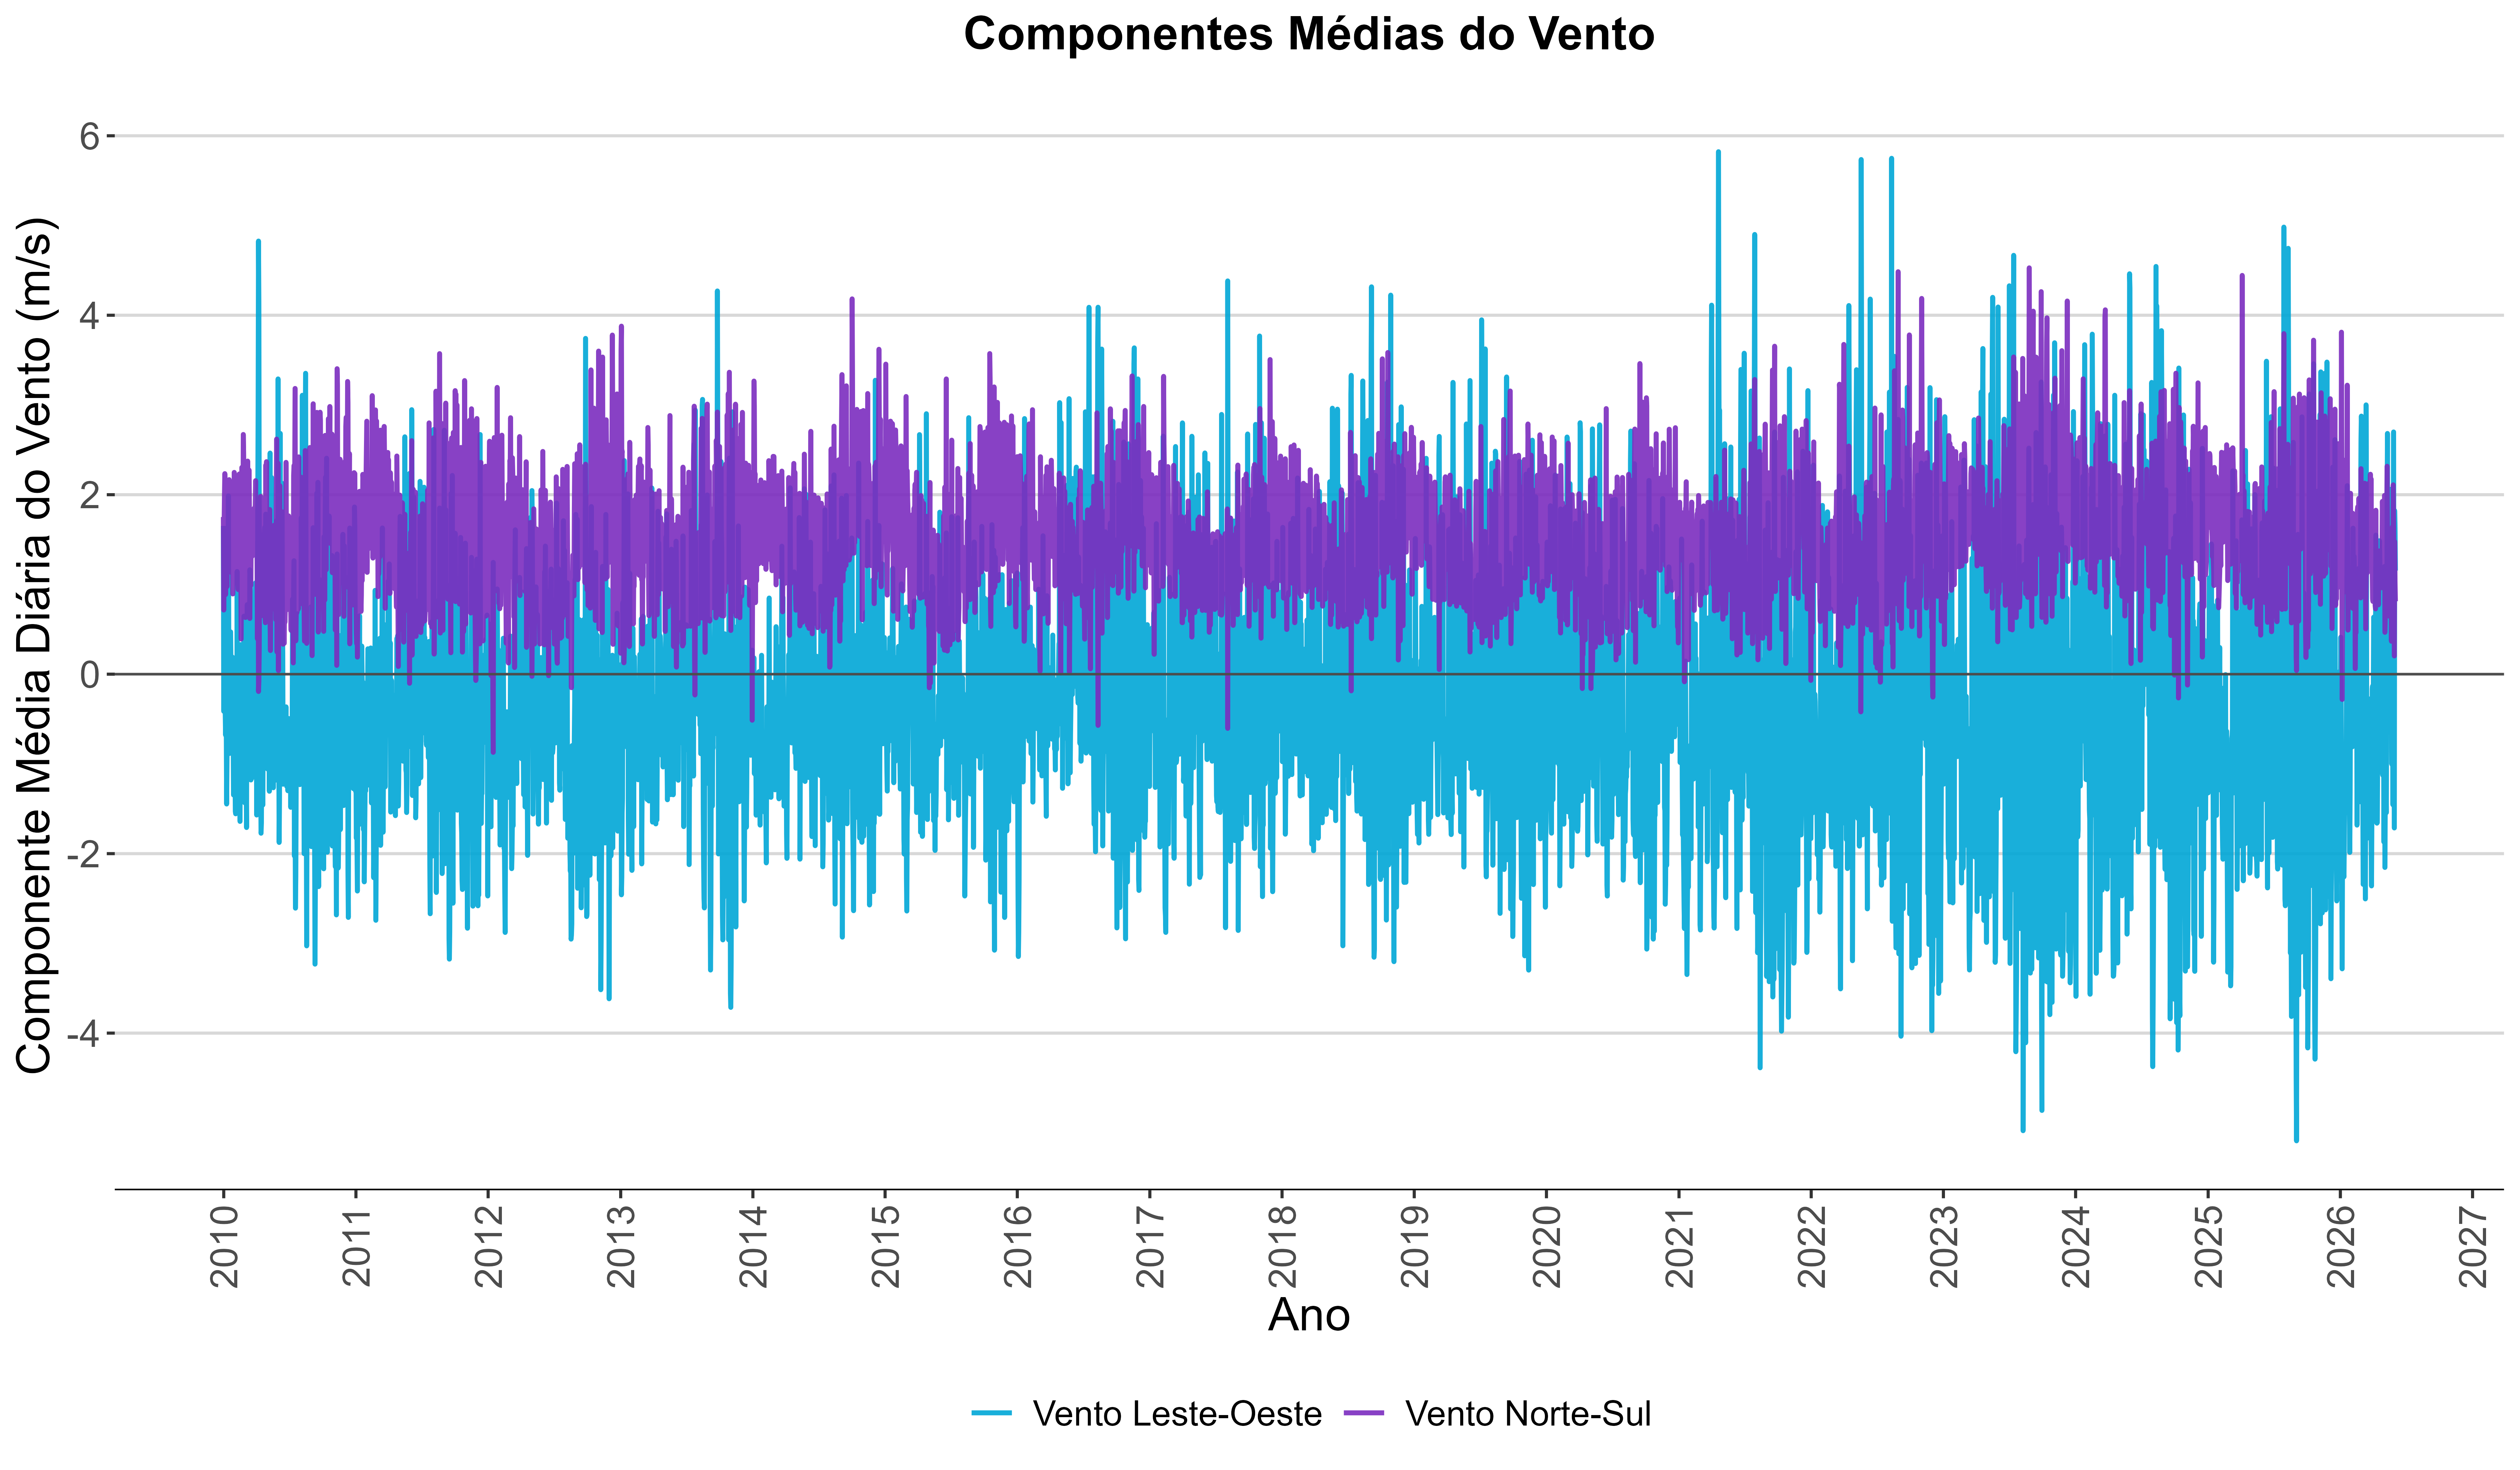
\includegraphics[keepaspectratio]{resultados/31_series_sobrepostas_componentes_vento.png}}

}

\caption{Componentes Médias do Vento}

\end{figure}%

\begin{quote}
\textbf{Comentário:} A sobreposição das componentes U (Leste-Oeste) e V
(Norte-Sul) permite observar que a componente U apresenta maior
variabilidade e picos mais intensos, indicando que os ventos que atingem
Niterói possuem essa dominância na direção.
\end{quote}

\begin{figure}[H]

{\centering \pandocbounded{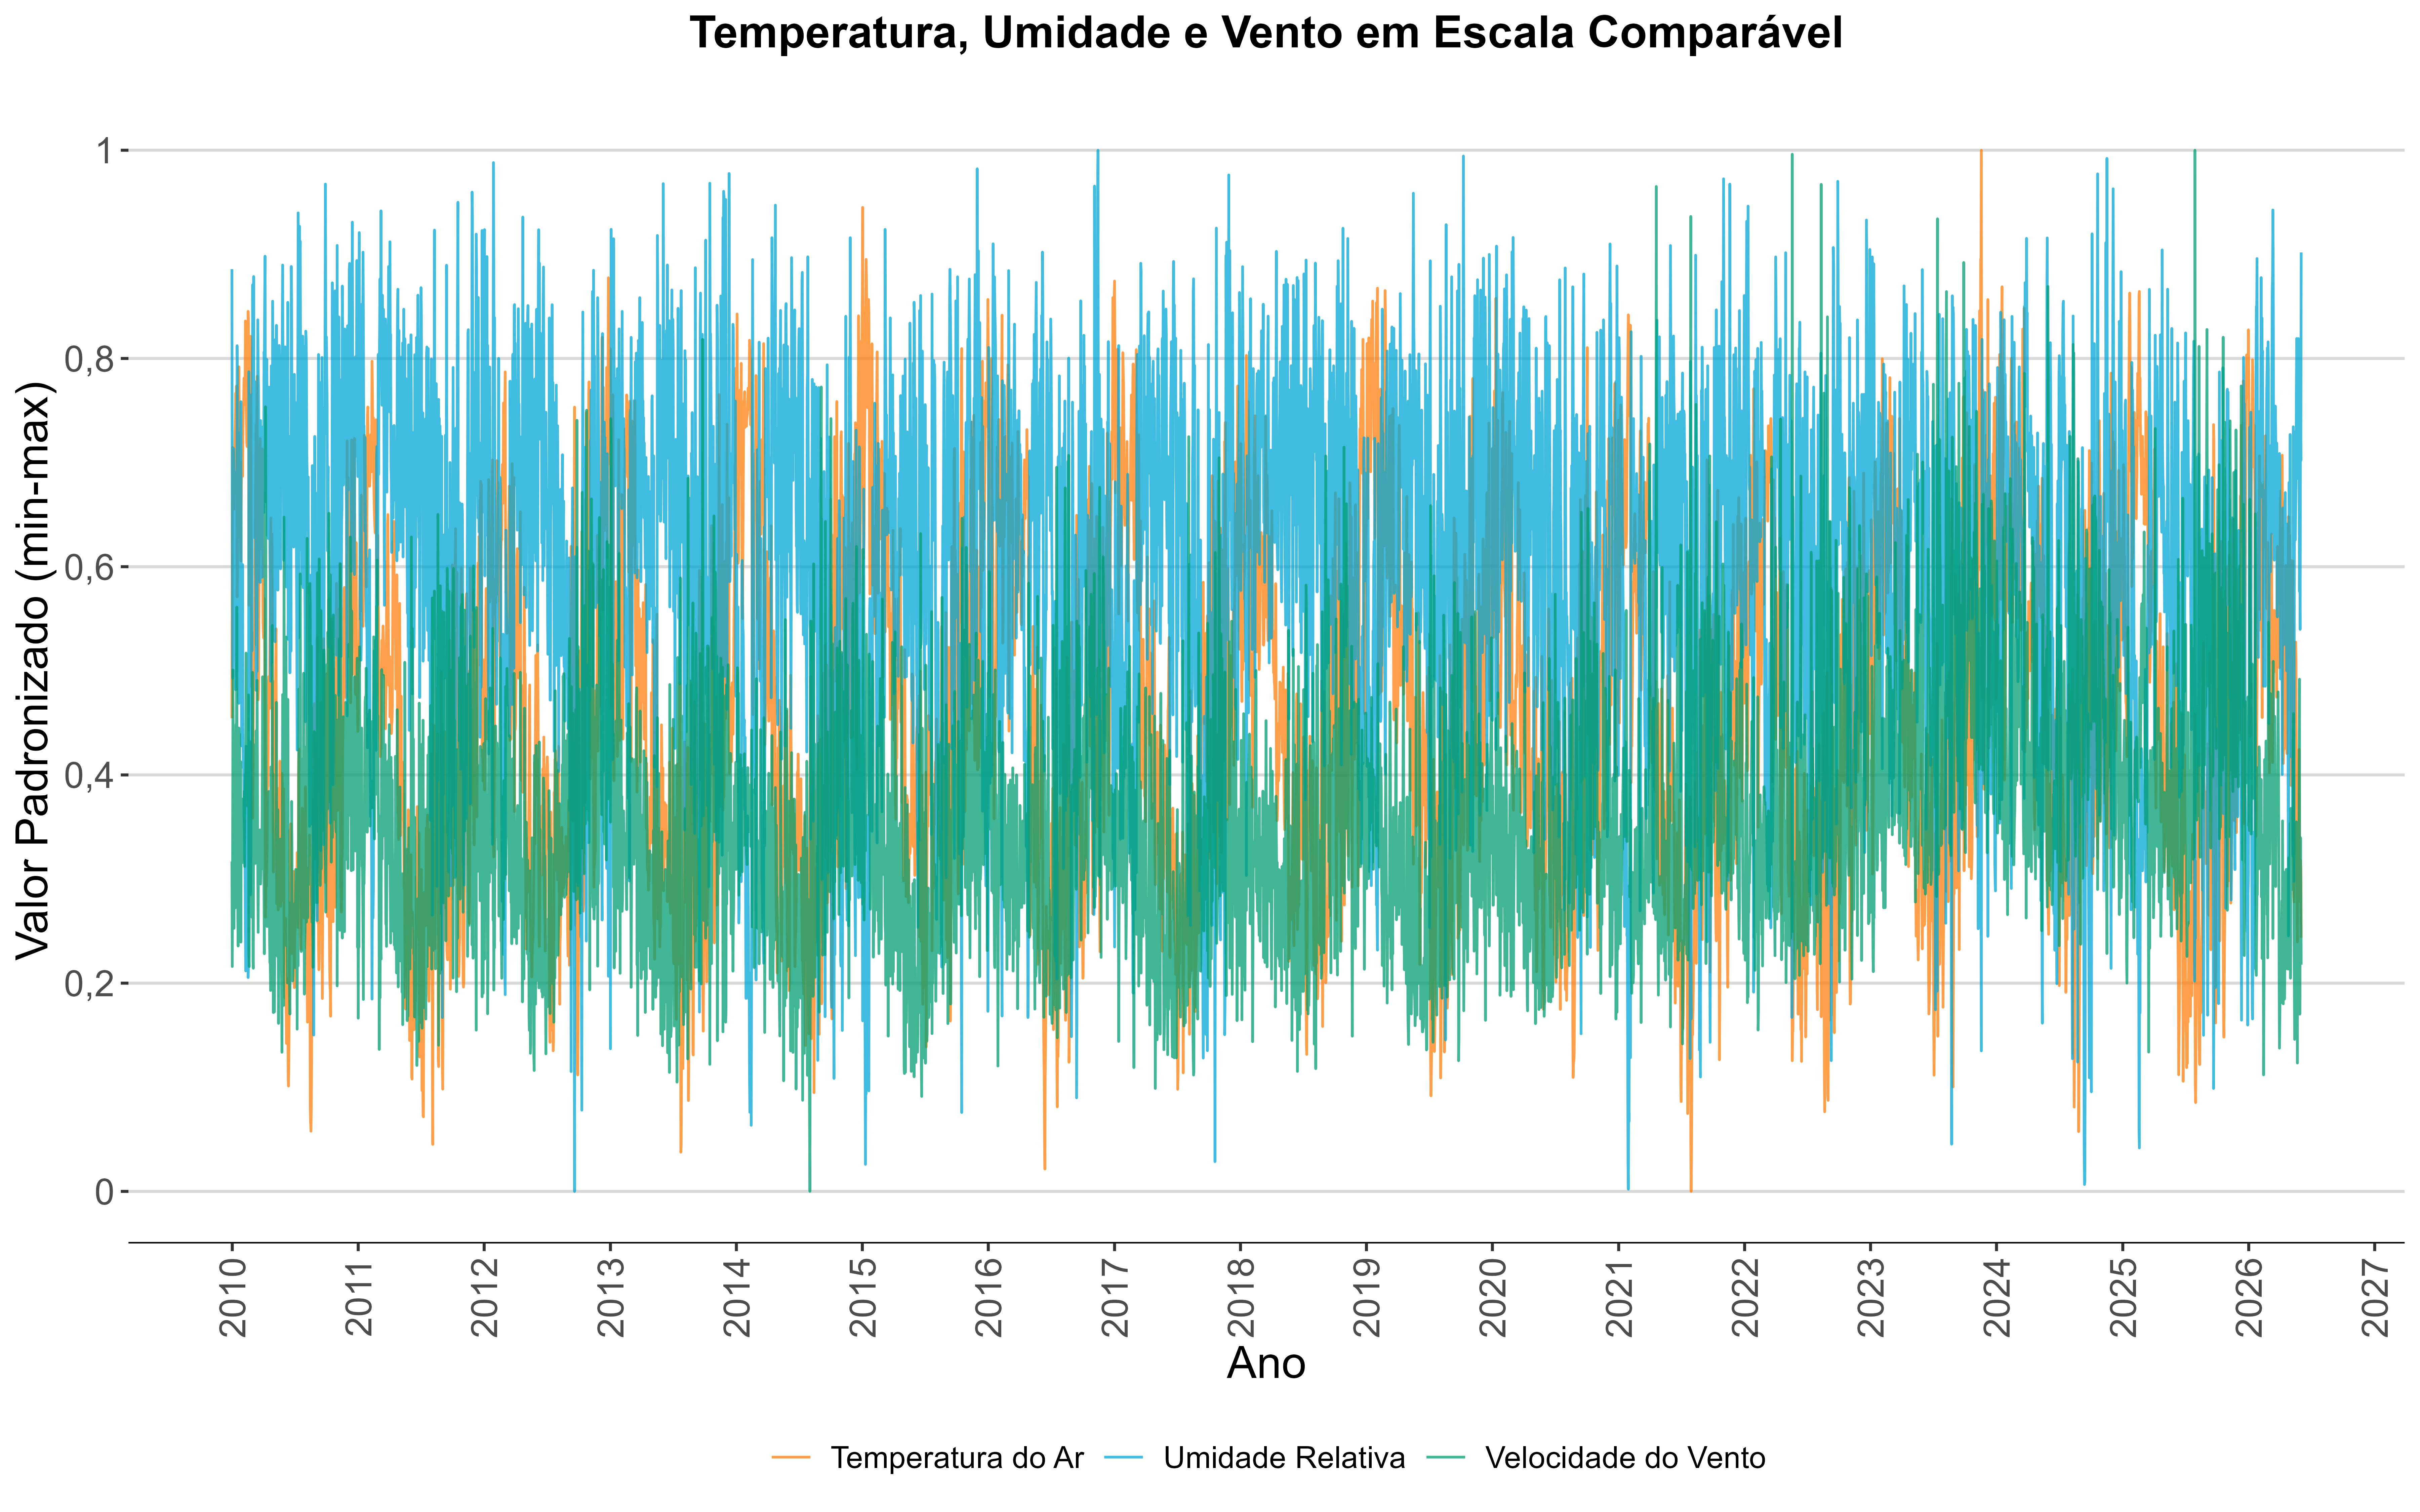
\includegraphics[keepaspectratio]{resultados/32_series_padronizadas_temperatura_umidade_vento.png}}

}

\caption{Temperatura, Umidade e Vento em Escala Comparável}

\end{figure}%

\begin{quote}
\textbf{Comentário:} Ao padronizar as variáveis, fica evidente o
comportamento em ``espelho'' entre a umidade relativa e a Velocidade do
Vento.
\end{quote}

\begin{figure}[H]

{\centering \pandocbounded{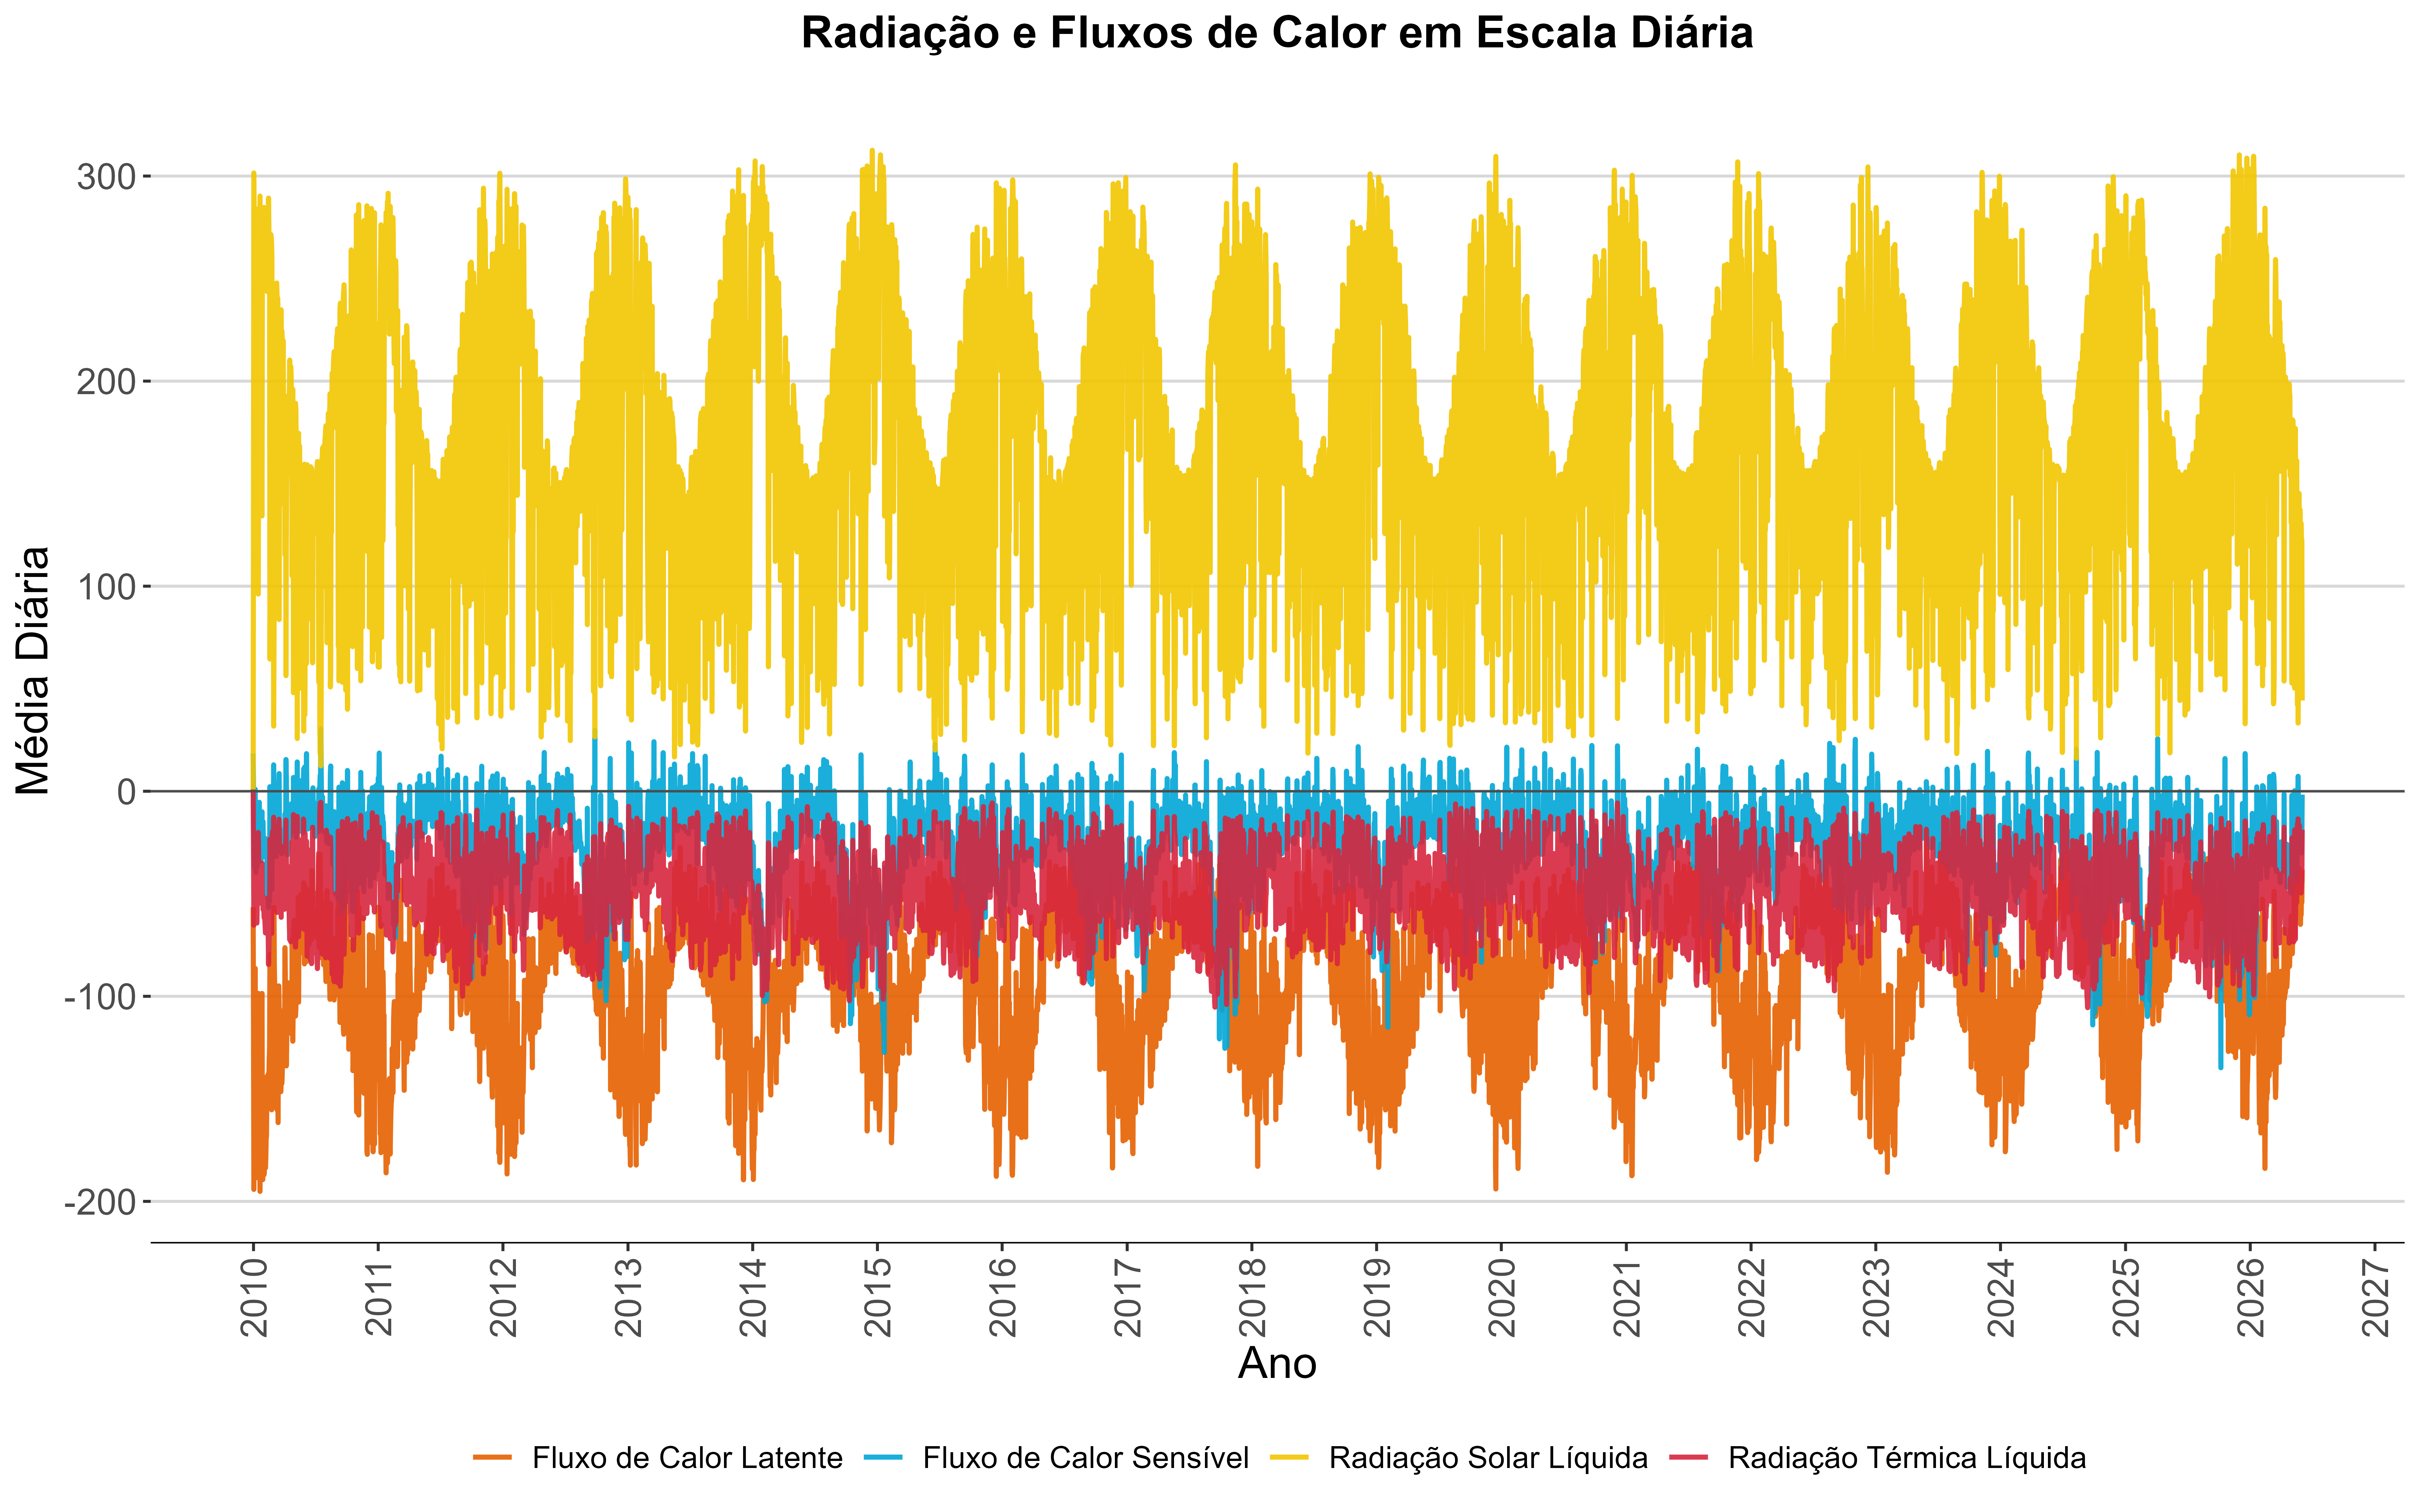
\includegraphics[keepaspectratio]{resultados/33_series_sobrepostas_radiacao_fluxos.png}}

}

\caption{Radiação e Fluxos de Calor em Escala Diária}

\end{figure}%

\begin{quote}
\textbf{Comentário:} O gráfico ilustra o balanço energético da
superfície. Enquanto a Radiação Solar Líquida é a principal fonte de
energia (positiva), os fluxos de calor latente, sensível e a radiação
térmica líquida atuam majoritariamente como perda de energia da
superfície para a atmosfera (valores negativos)
\end{quote}

\begin{figure}[H]

{\centering \pandocbounded{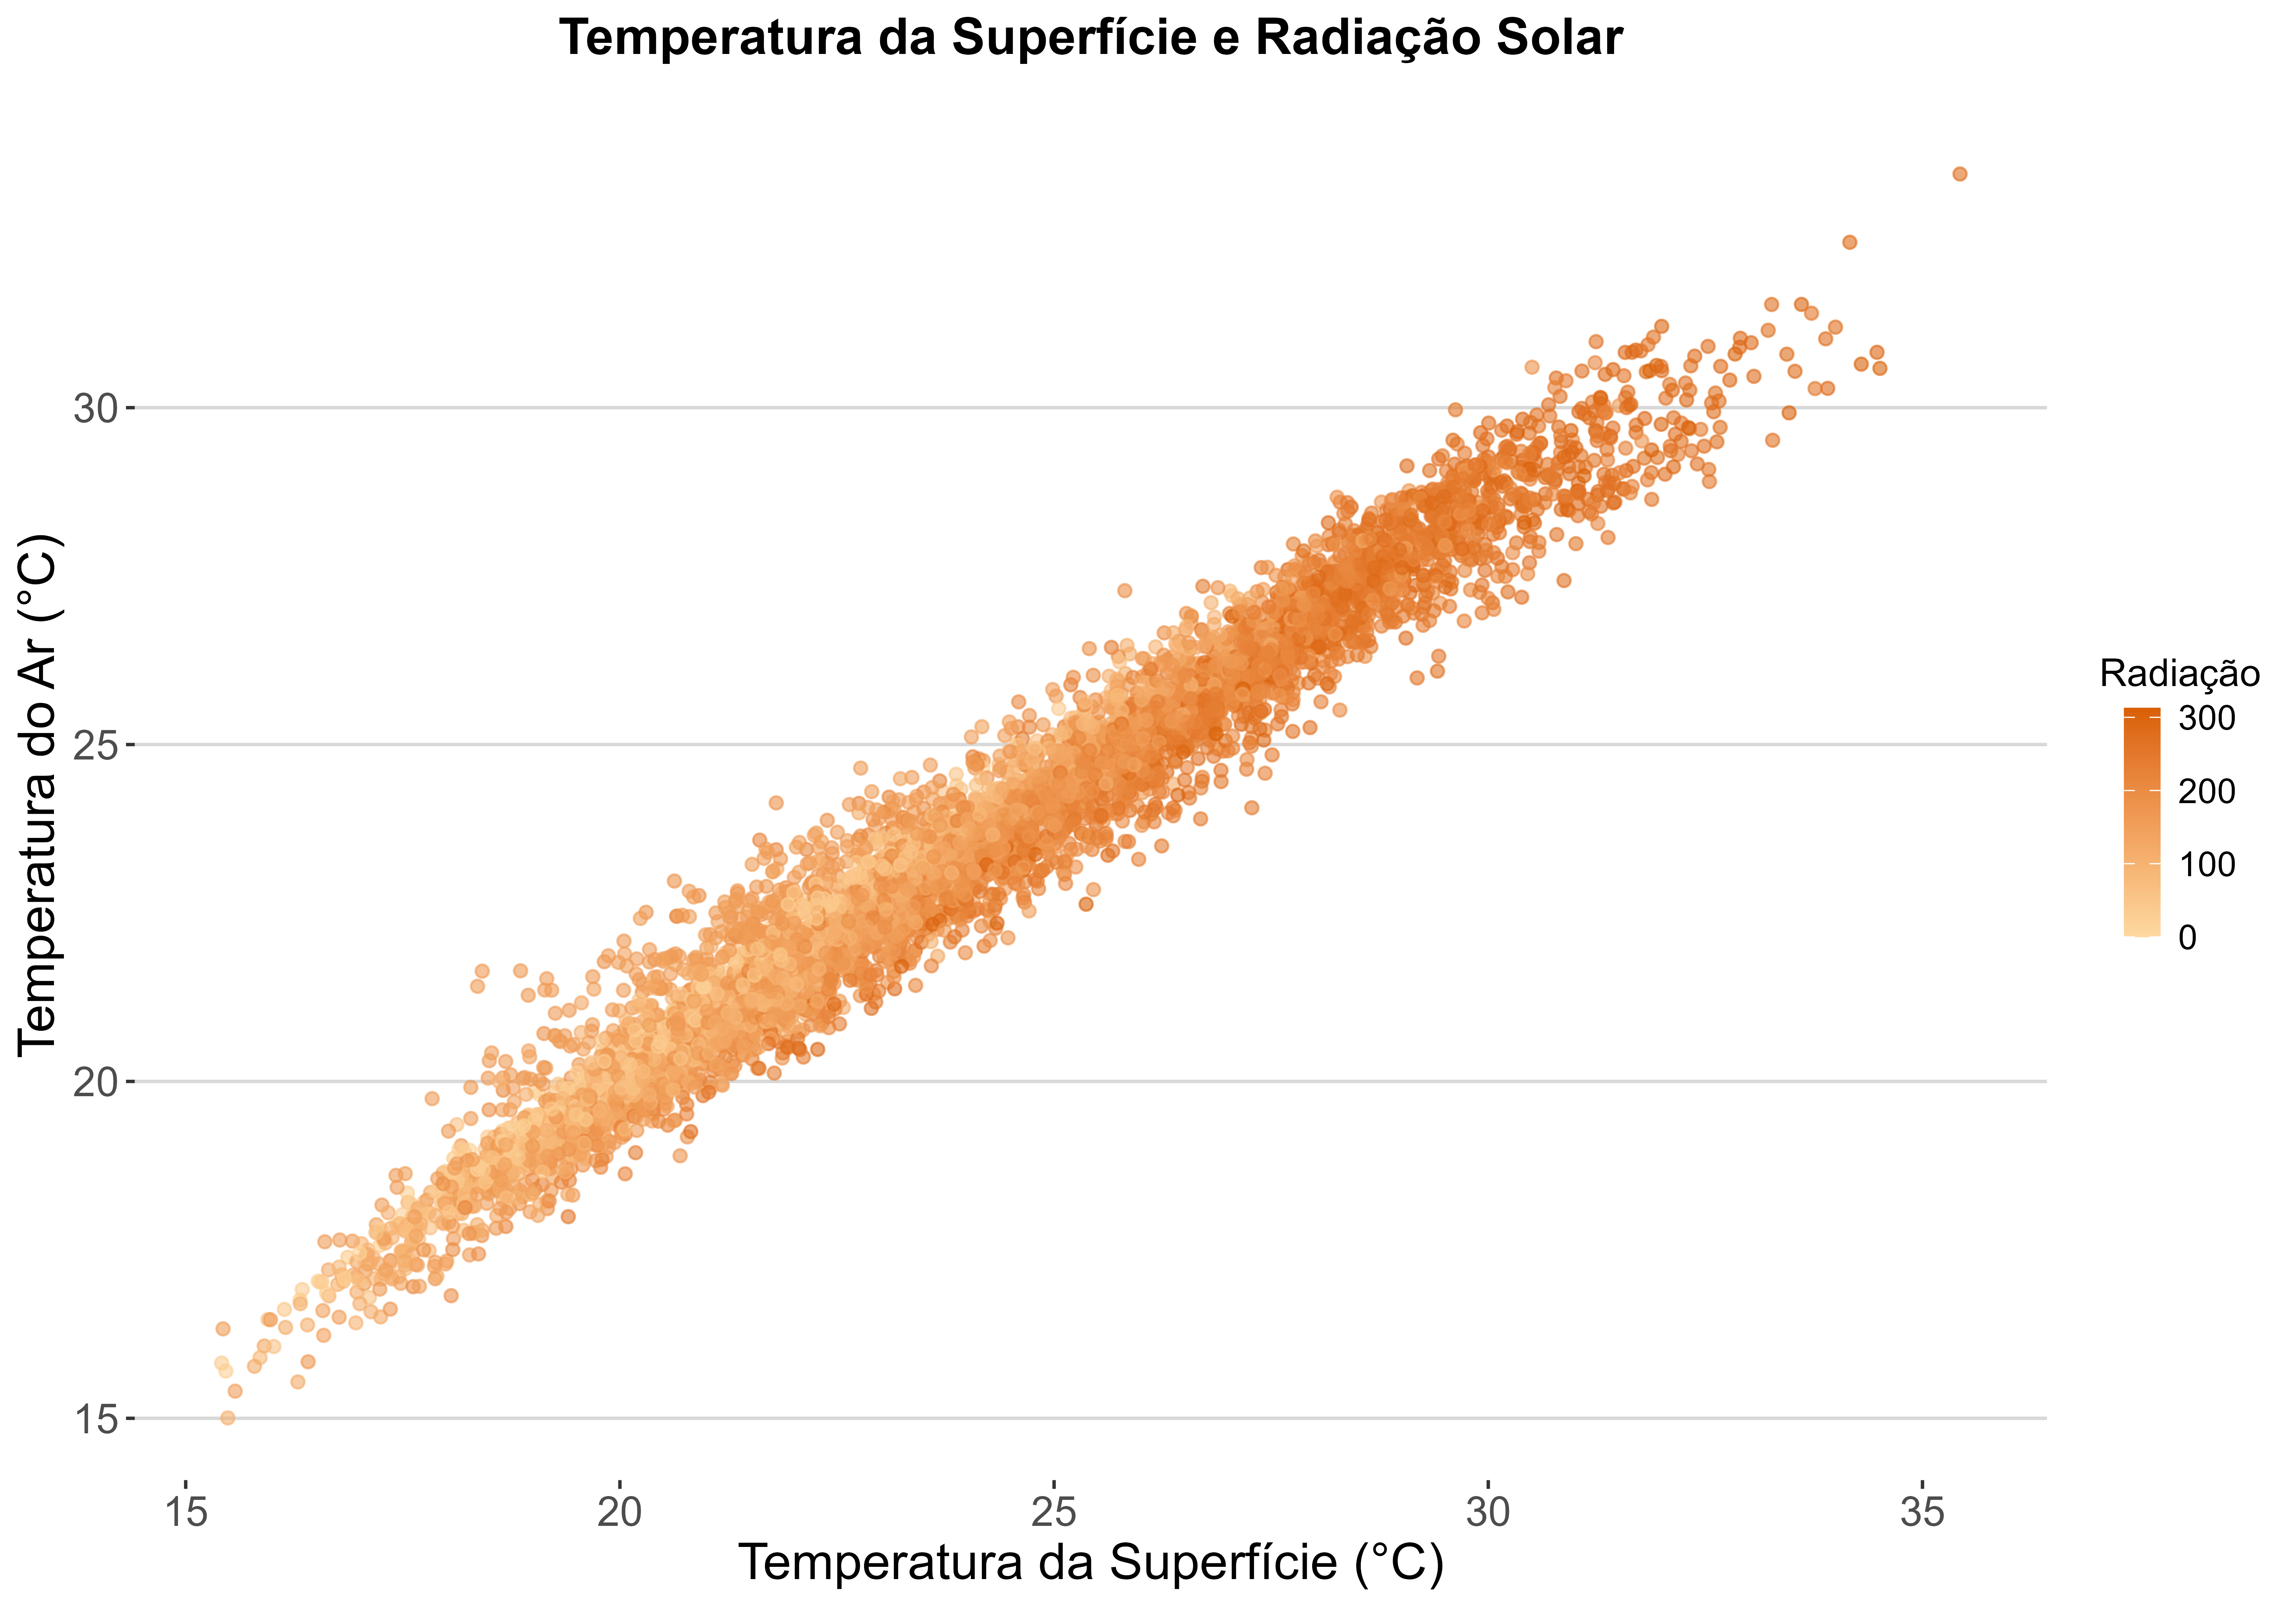
\includegraphics[keepaspectratio]{resultados/22_dispersao_temperatura_superficie_radiacao.png}}

}

\caption{Dispersão: Temperatura da Superfície e Radiação Solar}

\end{figure}%

\begin{quote}
\textbf{Comentário:} Confirmam uma forte relação linear positiva entre a
incidência solar e o aquecimento da superfície.
\end{quote}

\begin{figure}[H]

{\centering \pandocbounded{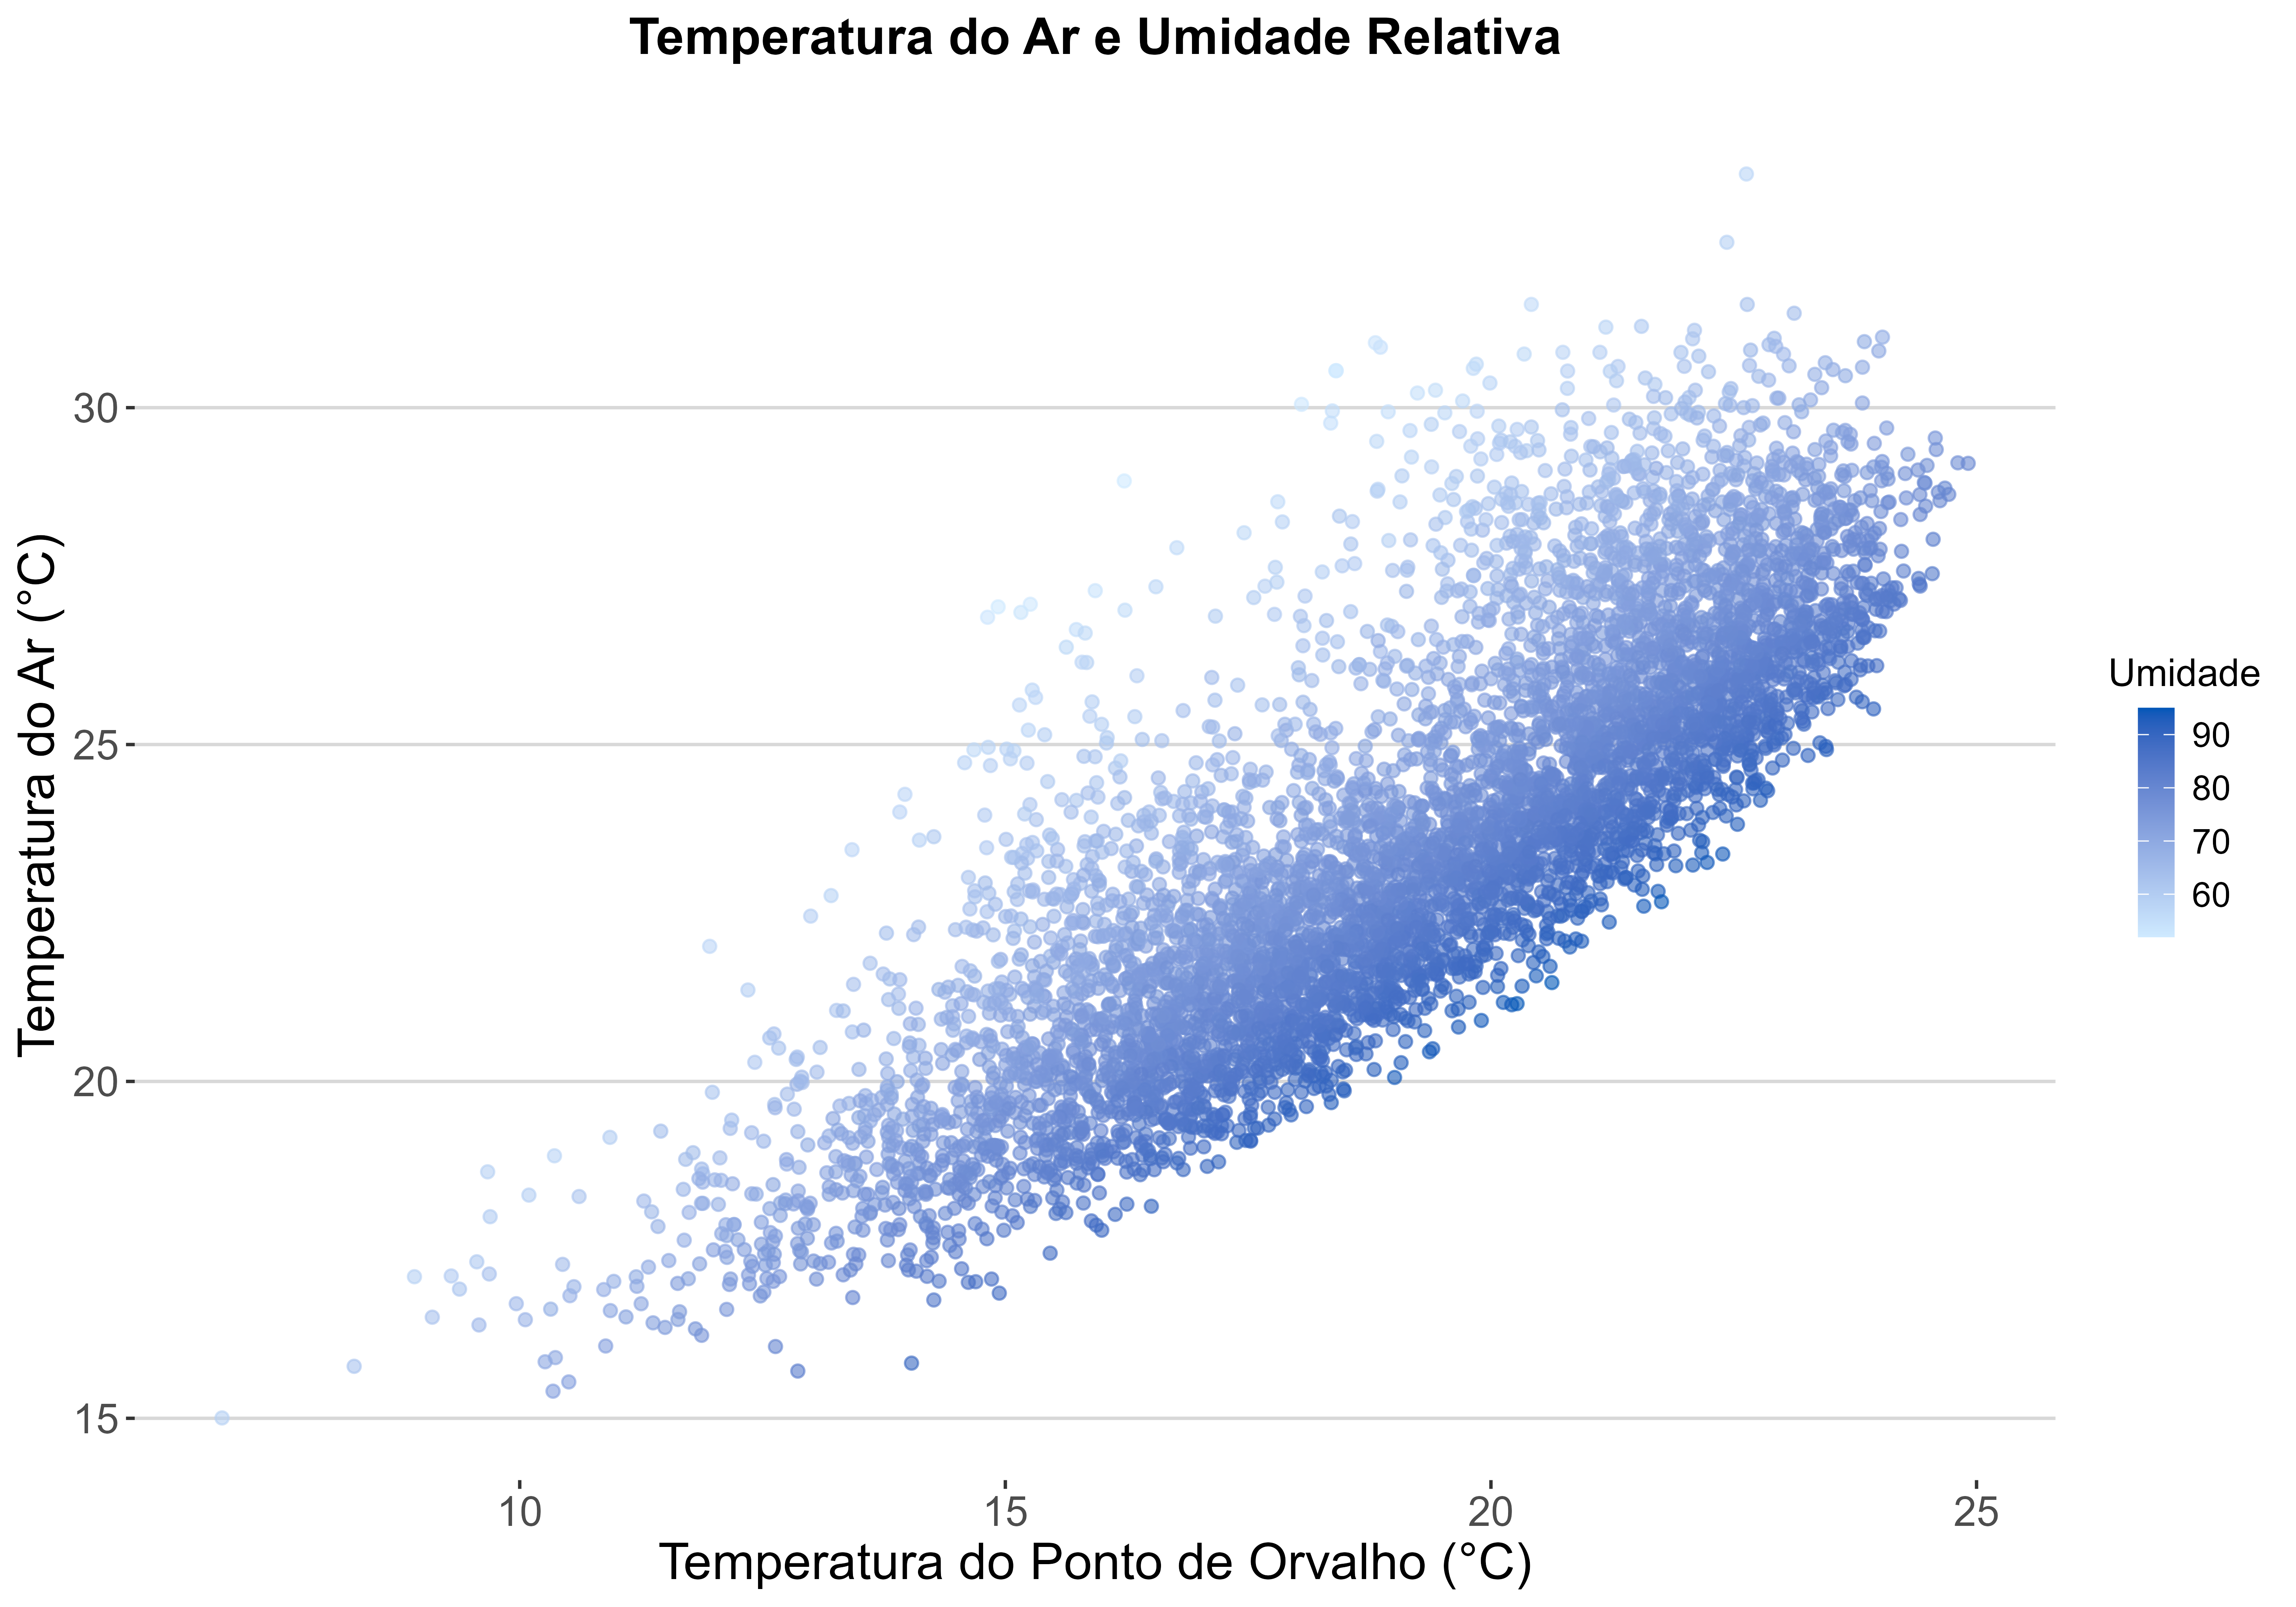
\includegraphics[keepaspectratio]{resultados/23_dispersao_temperatura_orvalho_umidade.png}}

}

\caption{Dispersão: Temperatura do Ar e Umidade Relativa}

\end{figure}%

\begin{quote}
\textbf{Comentário:} O gráfico de dispersão ratifica a correlação
negativa (-0,67) entre essas variáveis. Nota-se que temperaturas
elevadas (acima de 30°C) raramente ocorrem em condições de umidade muito
alta, o que é típico de regimes de ar mais seco ou períodos de forte
radiação solar
\end{quote}

\begin{figure}[H]

{\centering \pandocbounded{\includegraphics[keepaspectratio]{resultados/24_dispersao_radiacao_superficie_calor.png}}

}

\caption{Dispersão: Radiação Solar e Temperatura da Superfície}

\end{figure}%

\begin{figure}[H]

{\centering \pandocbounded{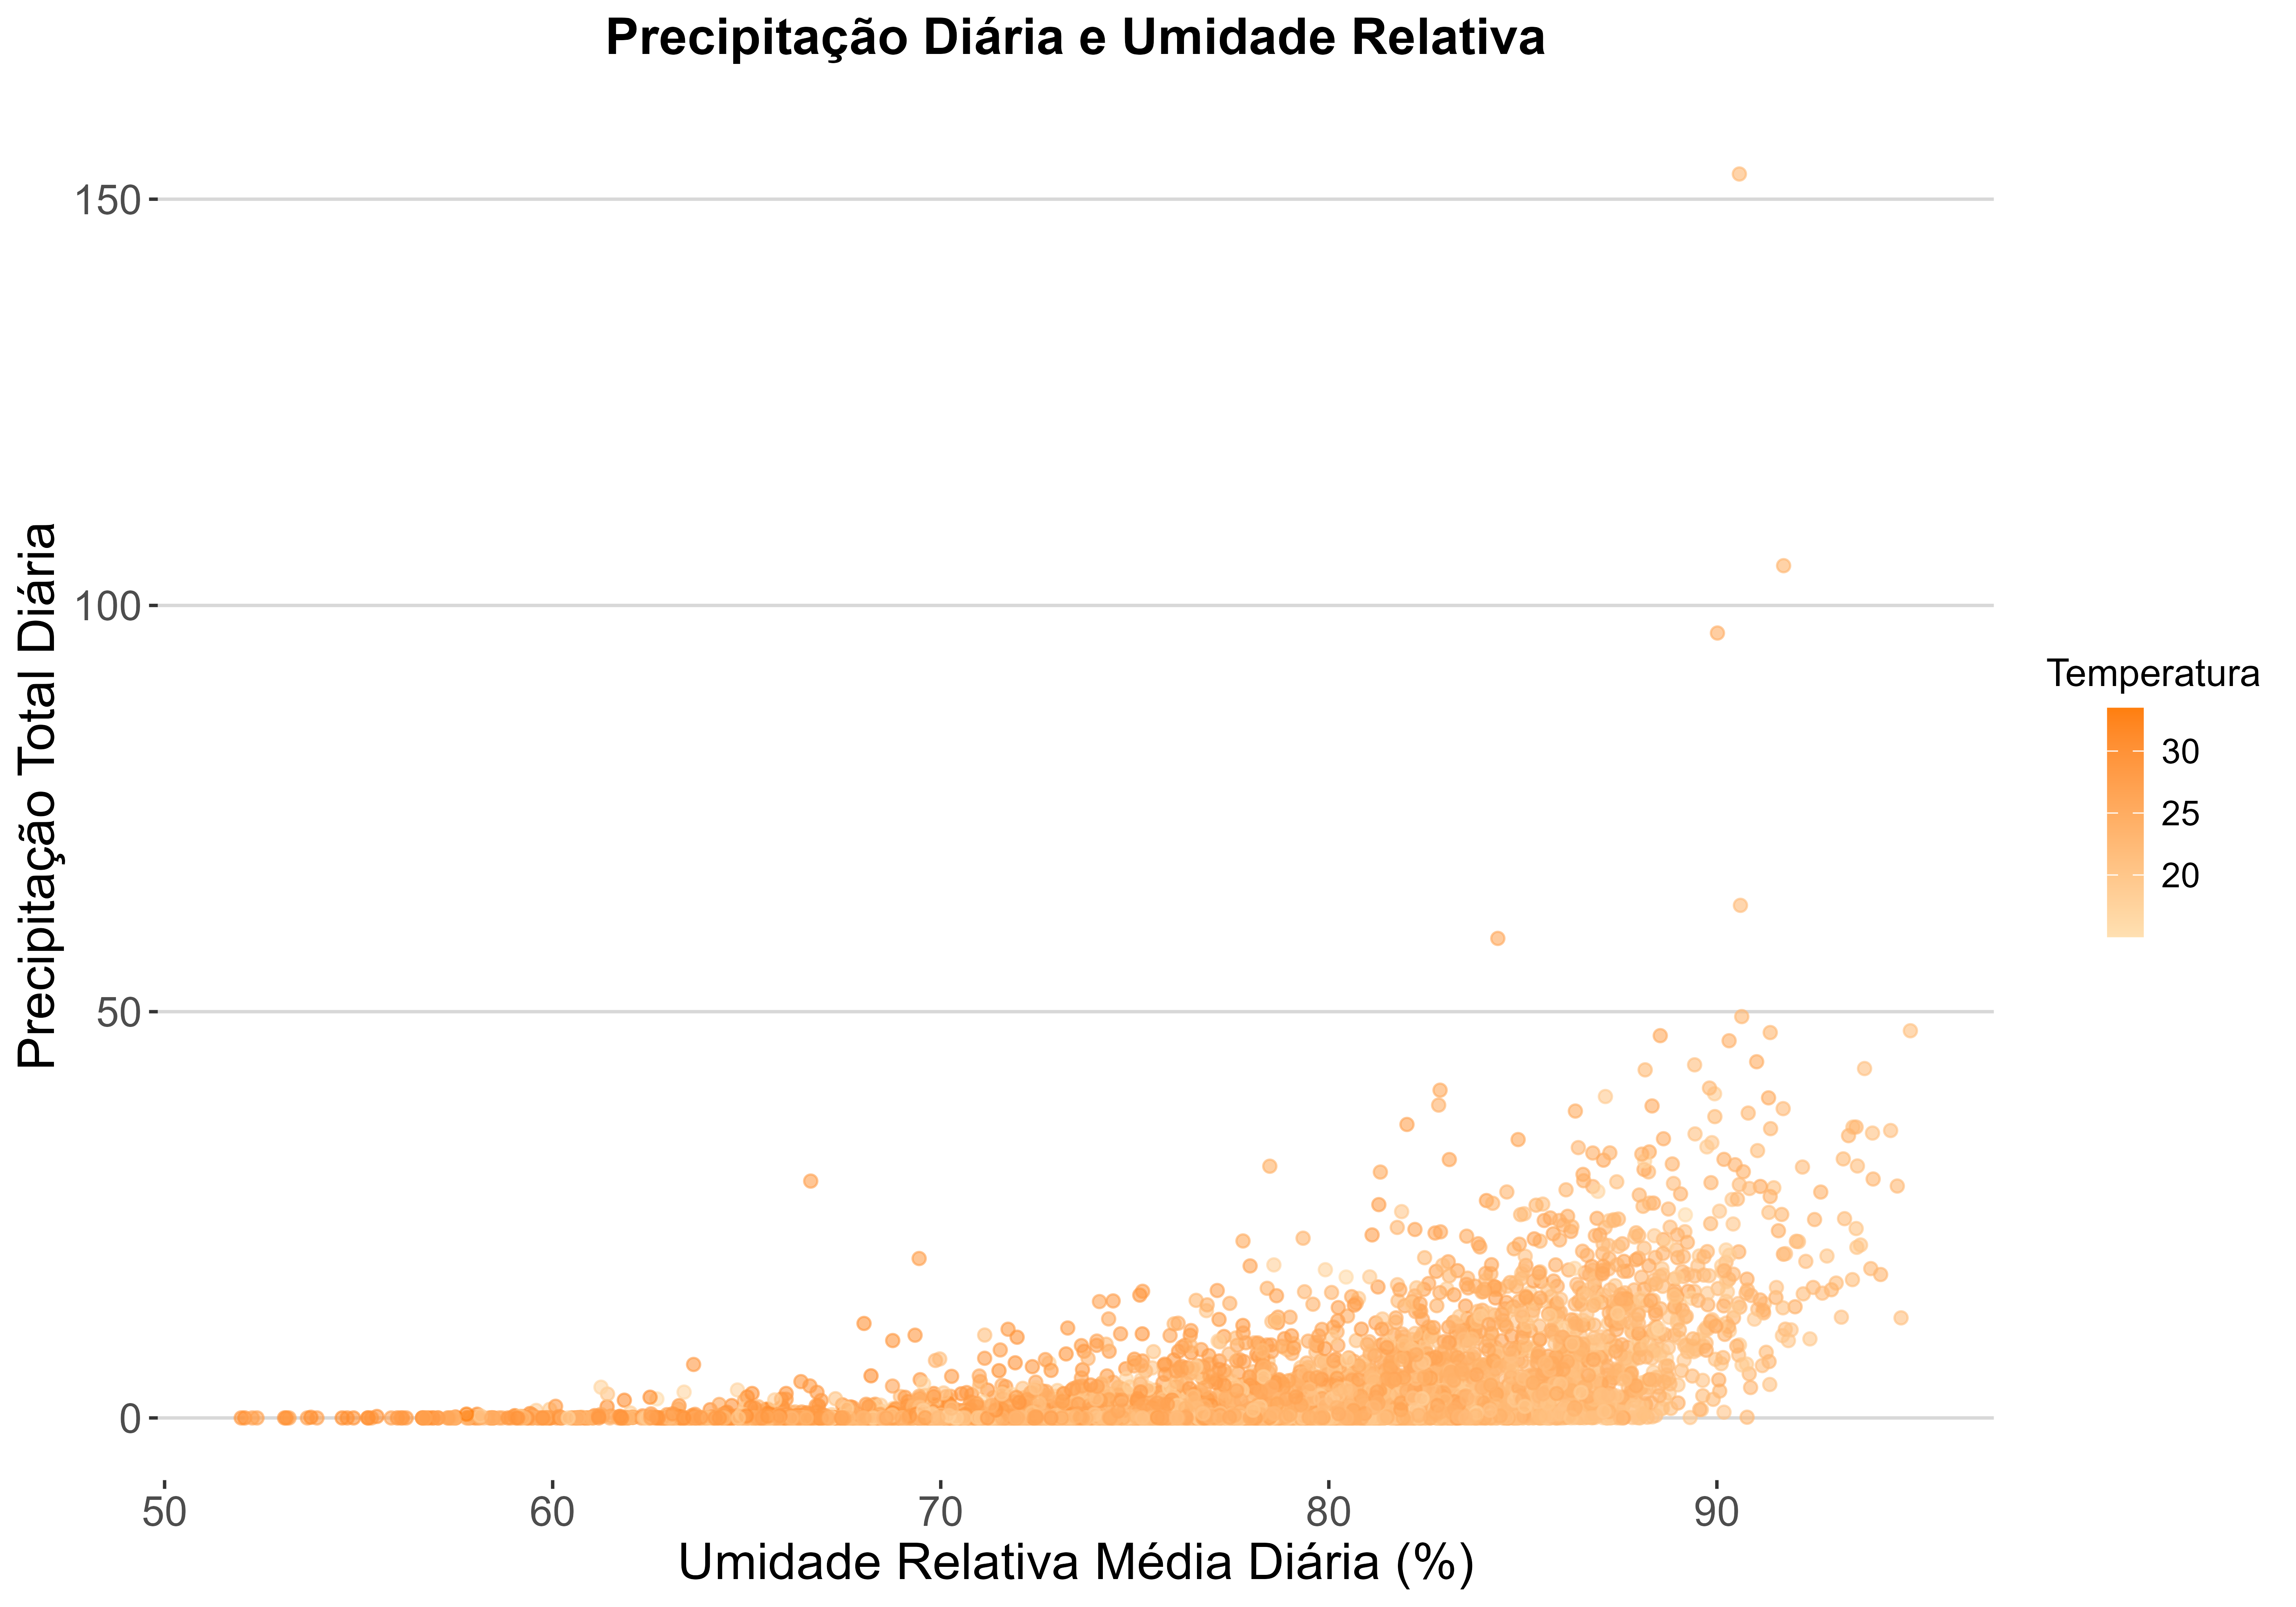
\includegraphics[keepaspectratio]{resultados/25_dispersao_umidade_chuva_temperatura.png}}

}

\caption{Dispersão: Precipitação Diária e Umidade Relativa}

\end{figure}%

\begin{quote}
\textbf{Comentário:} Este plot evidencia que eventos significativos de
precipitação são fenômenos de ``cauda'', ocorrendo quase exclusivamente
quando a umidade relativa diária está acima de 80-90\%
\end{quote}

\begin{figure}[H]

{\centering \pandocbounded{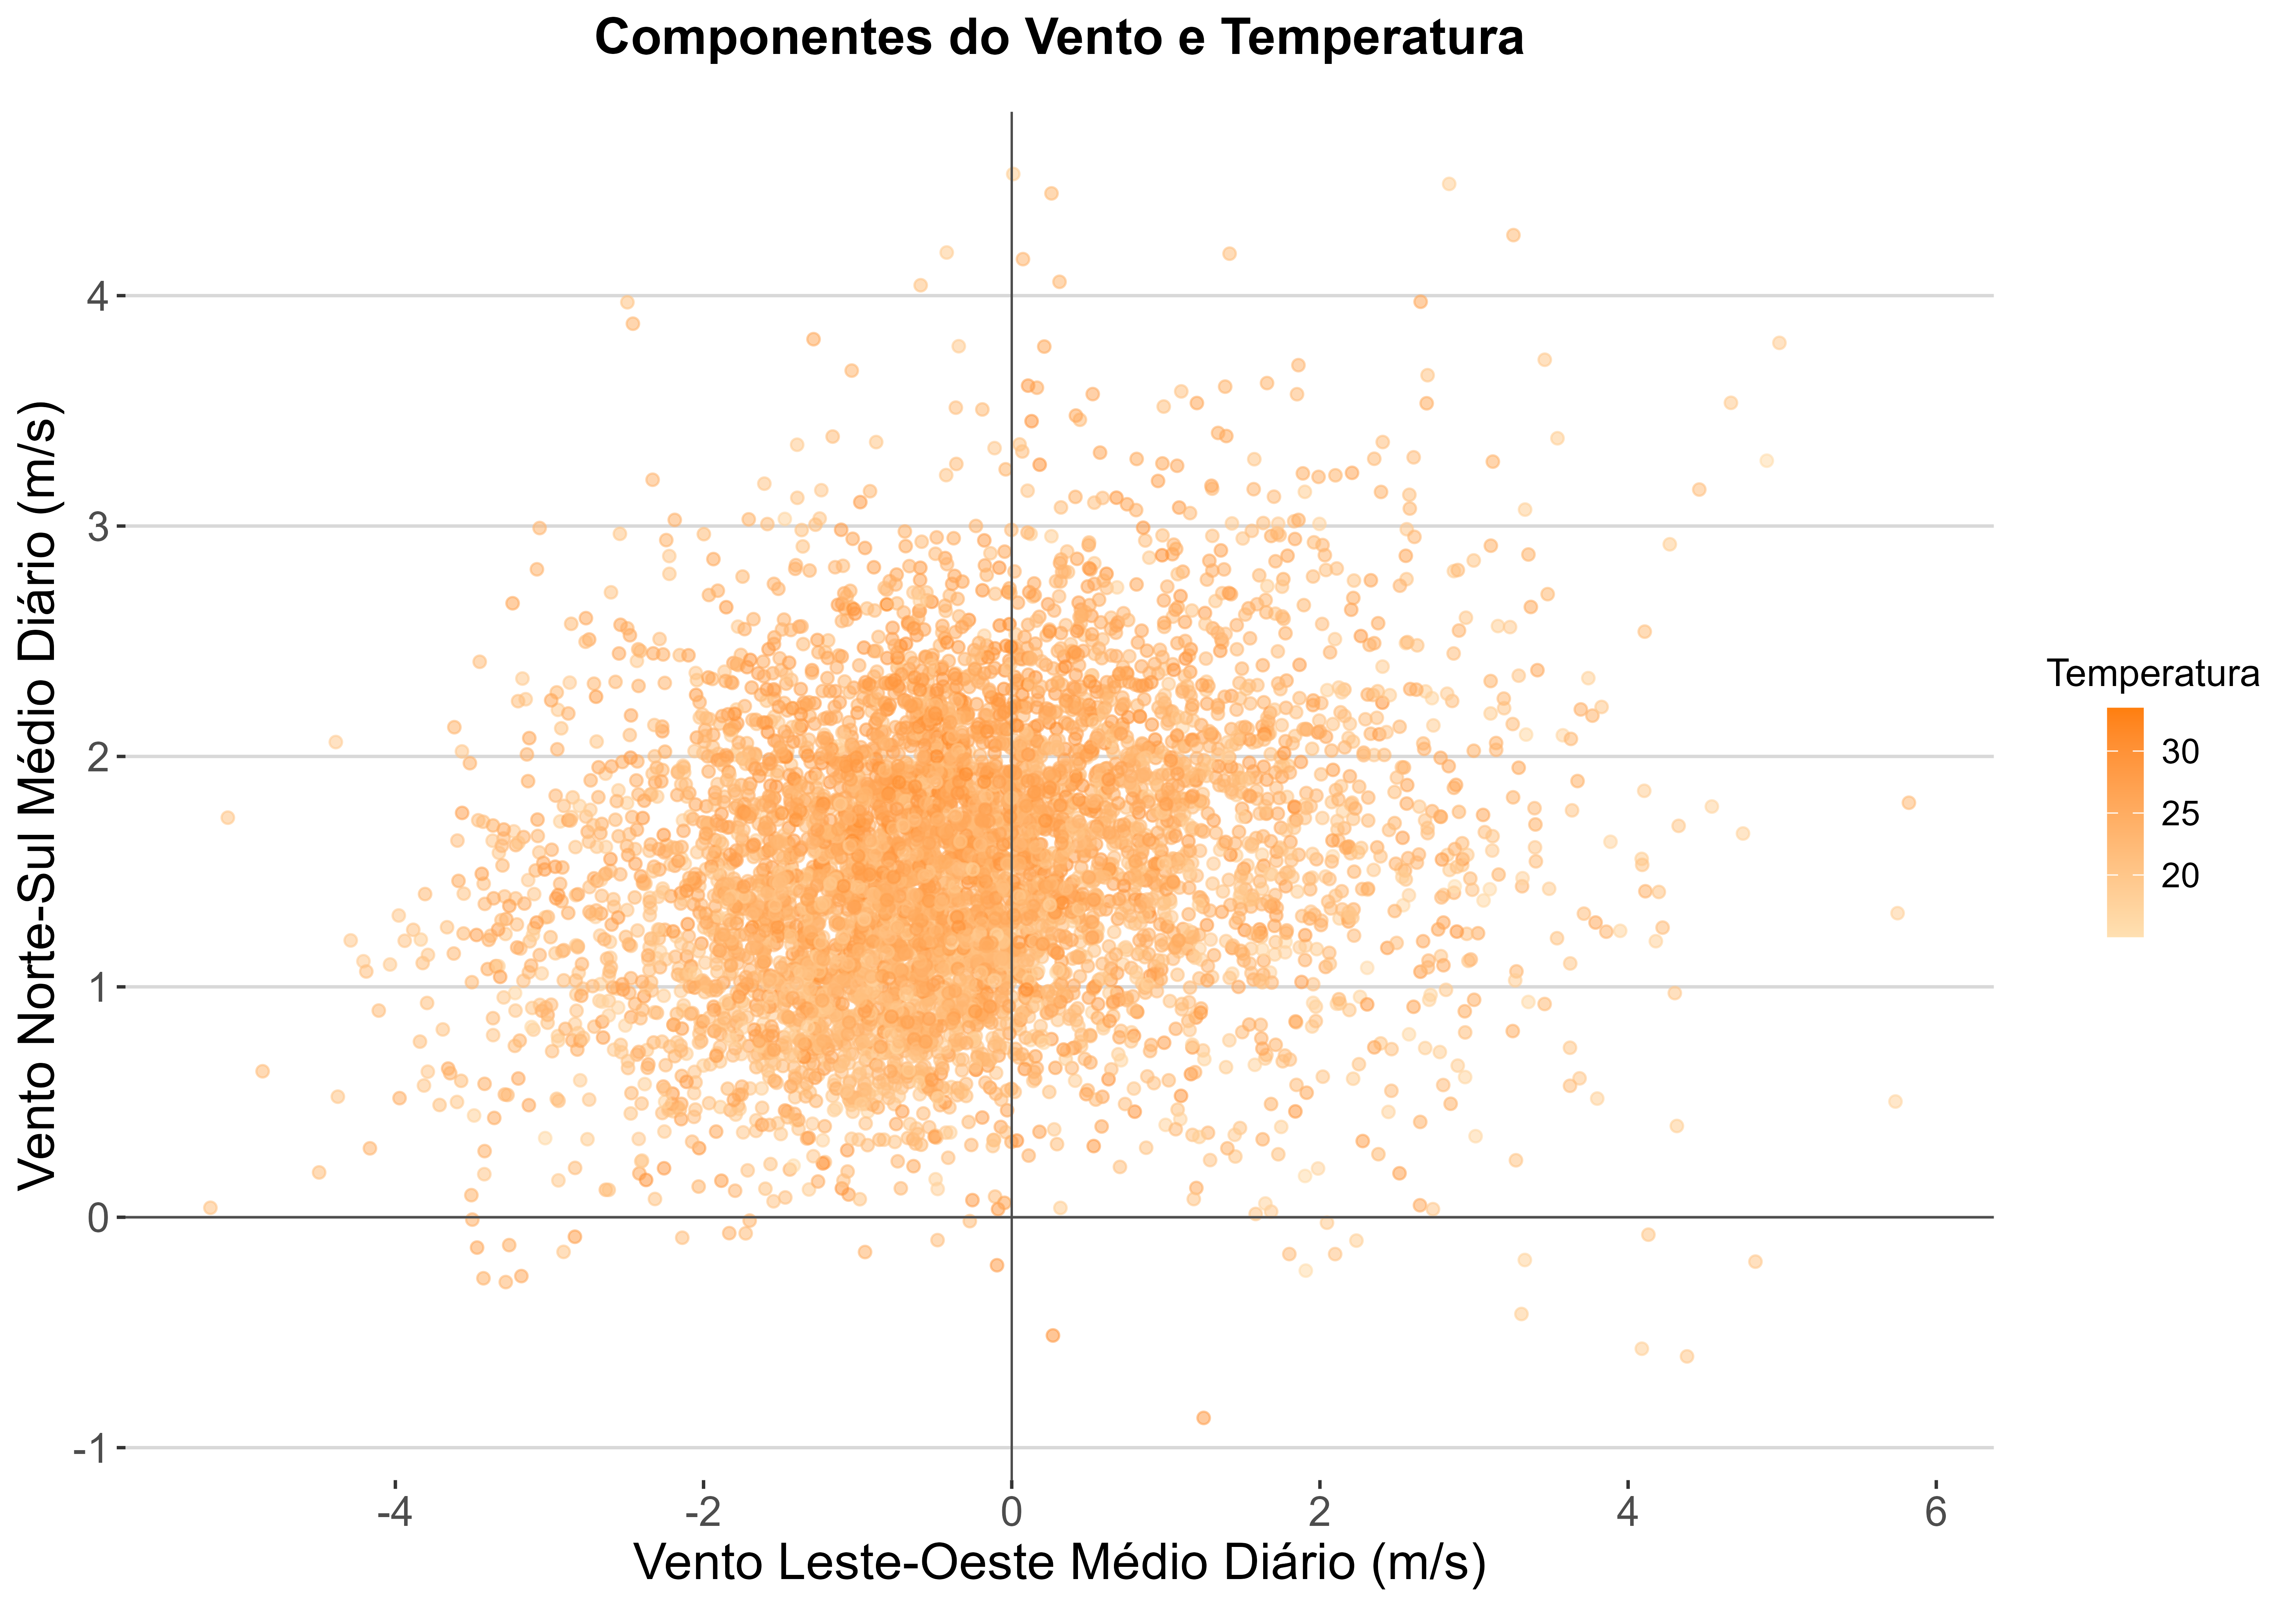
\includegraphics[keepaspectratio]{resultados/26_dispersao_vento_temperatura.png}}

}

\caption{Dispersão: Componentes do Vento e Temperatura}

\end{figure}%

\begin{quote}
\textbf{Comentário:} A dispersão sugere que não há uma relação linear
simples entre a direção do vento e a temperatura, mas permite
identificar agrupamentos que podem estar associados a brisas marítimas
ou frentes frias
\end{quote}

\begin{figure}[H]

{\centering \pandocbounded{\includegraphics[keepaspectratio]{resultados/27_matriz_correlacao.png}}

}

\caption{Matriz de Correlação Entre as Variáveis Meteorológicas}

\end{figure}%

\begin{quote}
\textbf{Comentário:} É o resumo estatístico da seção. Destaca-se a
correlação quase perfeita (0,96) entre a temperatura do ar e a da
superfície, validando esta última como o preditor mais robusto para o
modelo LSTM . Além disso, a forte correlação entre os fluxos de calor
latente e sensível (0,80) reforça a consistência física dos dados de
reanálise
\end{quote}

\paragraph{Principais Achados}\label{principais-achados-13}

As três séries de temperatura (ar, superfície e orvalho) evoluem de
forma \textbf{altamente sincronizada}, com a temperatura da superfície
apresentando maior amplitude e os valores de orvalho funcionando como
piso térmico. A diferença entre a temperatura do ar e a do orvalho é um
indicador direto do déficit de pressão de vapor, variando de quase zero
nos dias úmidos a mais de 10 °C nos dias secos de inverno.

As componentes U e V do vento mostram comportamentos
\textbf{descorrelacionados entre si}, com U mais estável e V mais
volátil. A série padronizada de temperatura, umidade e vento confirma a
anticorrelação entre temperatura e umidade: quando a temperatura sobe
(verão), a umidade relativa cai ligeiramente, e vice-versa no inverno.

Radiação solar, fluxo de calor latente e fluxo sensível evoluem em
\textbf{fase}, com os maiores valores no verão. A radiação térmica
líquida apresenta comportamento oposto (mais negativa no inverno),
completando o balanço energético da superfície.

Os gráficos de dispersão confirmam relações físicas esperadas: forte
correlação positiva entre temperatura do ar e da superfície (mediada
pela radiação solar), correlação positiva entre temperatura do orvalho e
umidade relativa, e dispersão crescente entre precipitação e umidade
(eventos extremos de chuva ocorrem em ampla faixa de umidade).

A \textbf{matriz de correlação} destaca as correlações mais relevantes
para a modelagem: temperatura do ar correlaciona-se com temperatura da
superfície (0,95), umidade relativa(-0,67), Radiação Solar
Líquida(0,66), e outras. Com metor correlação com a Precipitação e o
Vento Leste-Oeste.

\section{Definição da Base de Treino e
Teste}\label{definiuxe7uxe3o-da-base-de-treino-e-teste}

\begin{figure}[H]

{\centering \pandocbounded{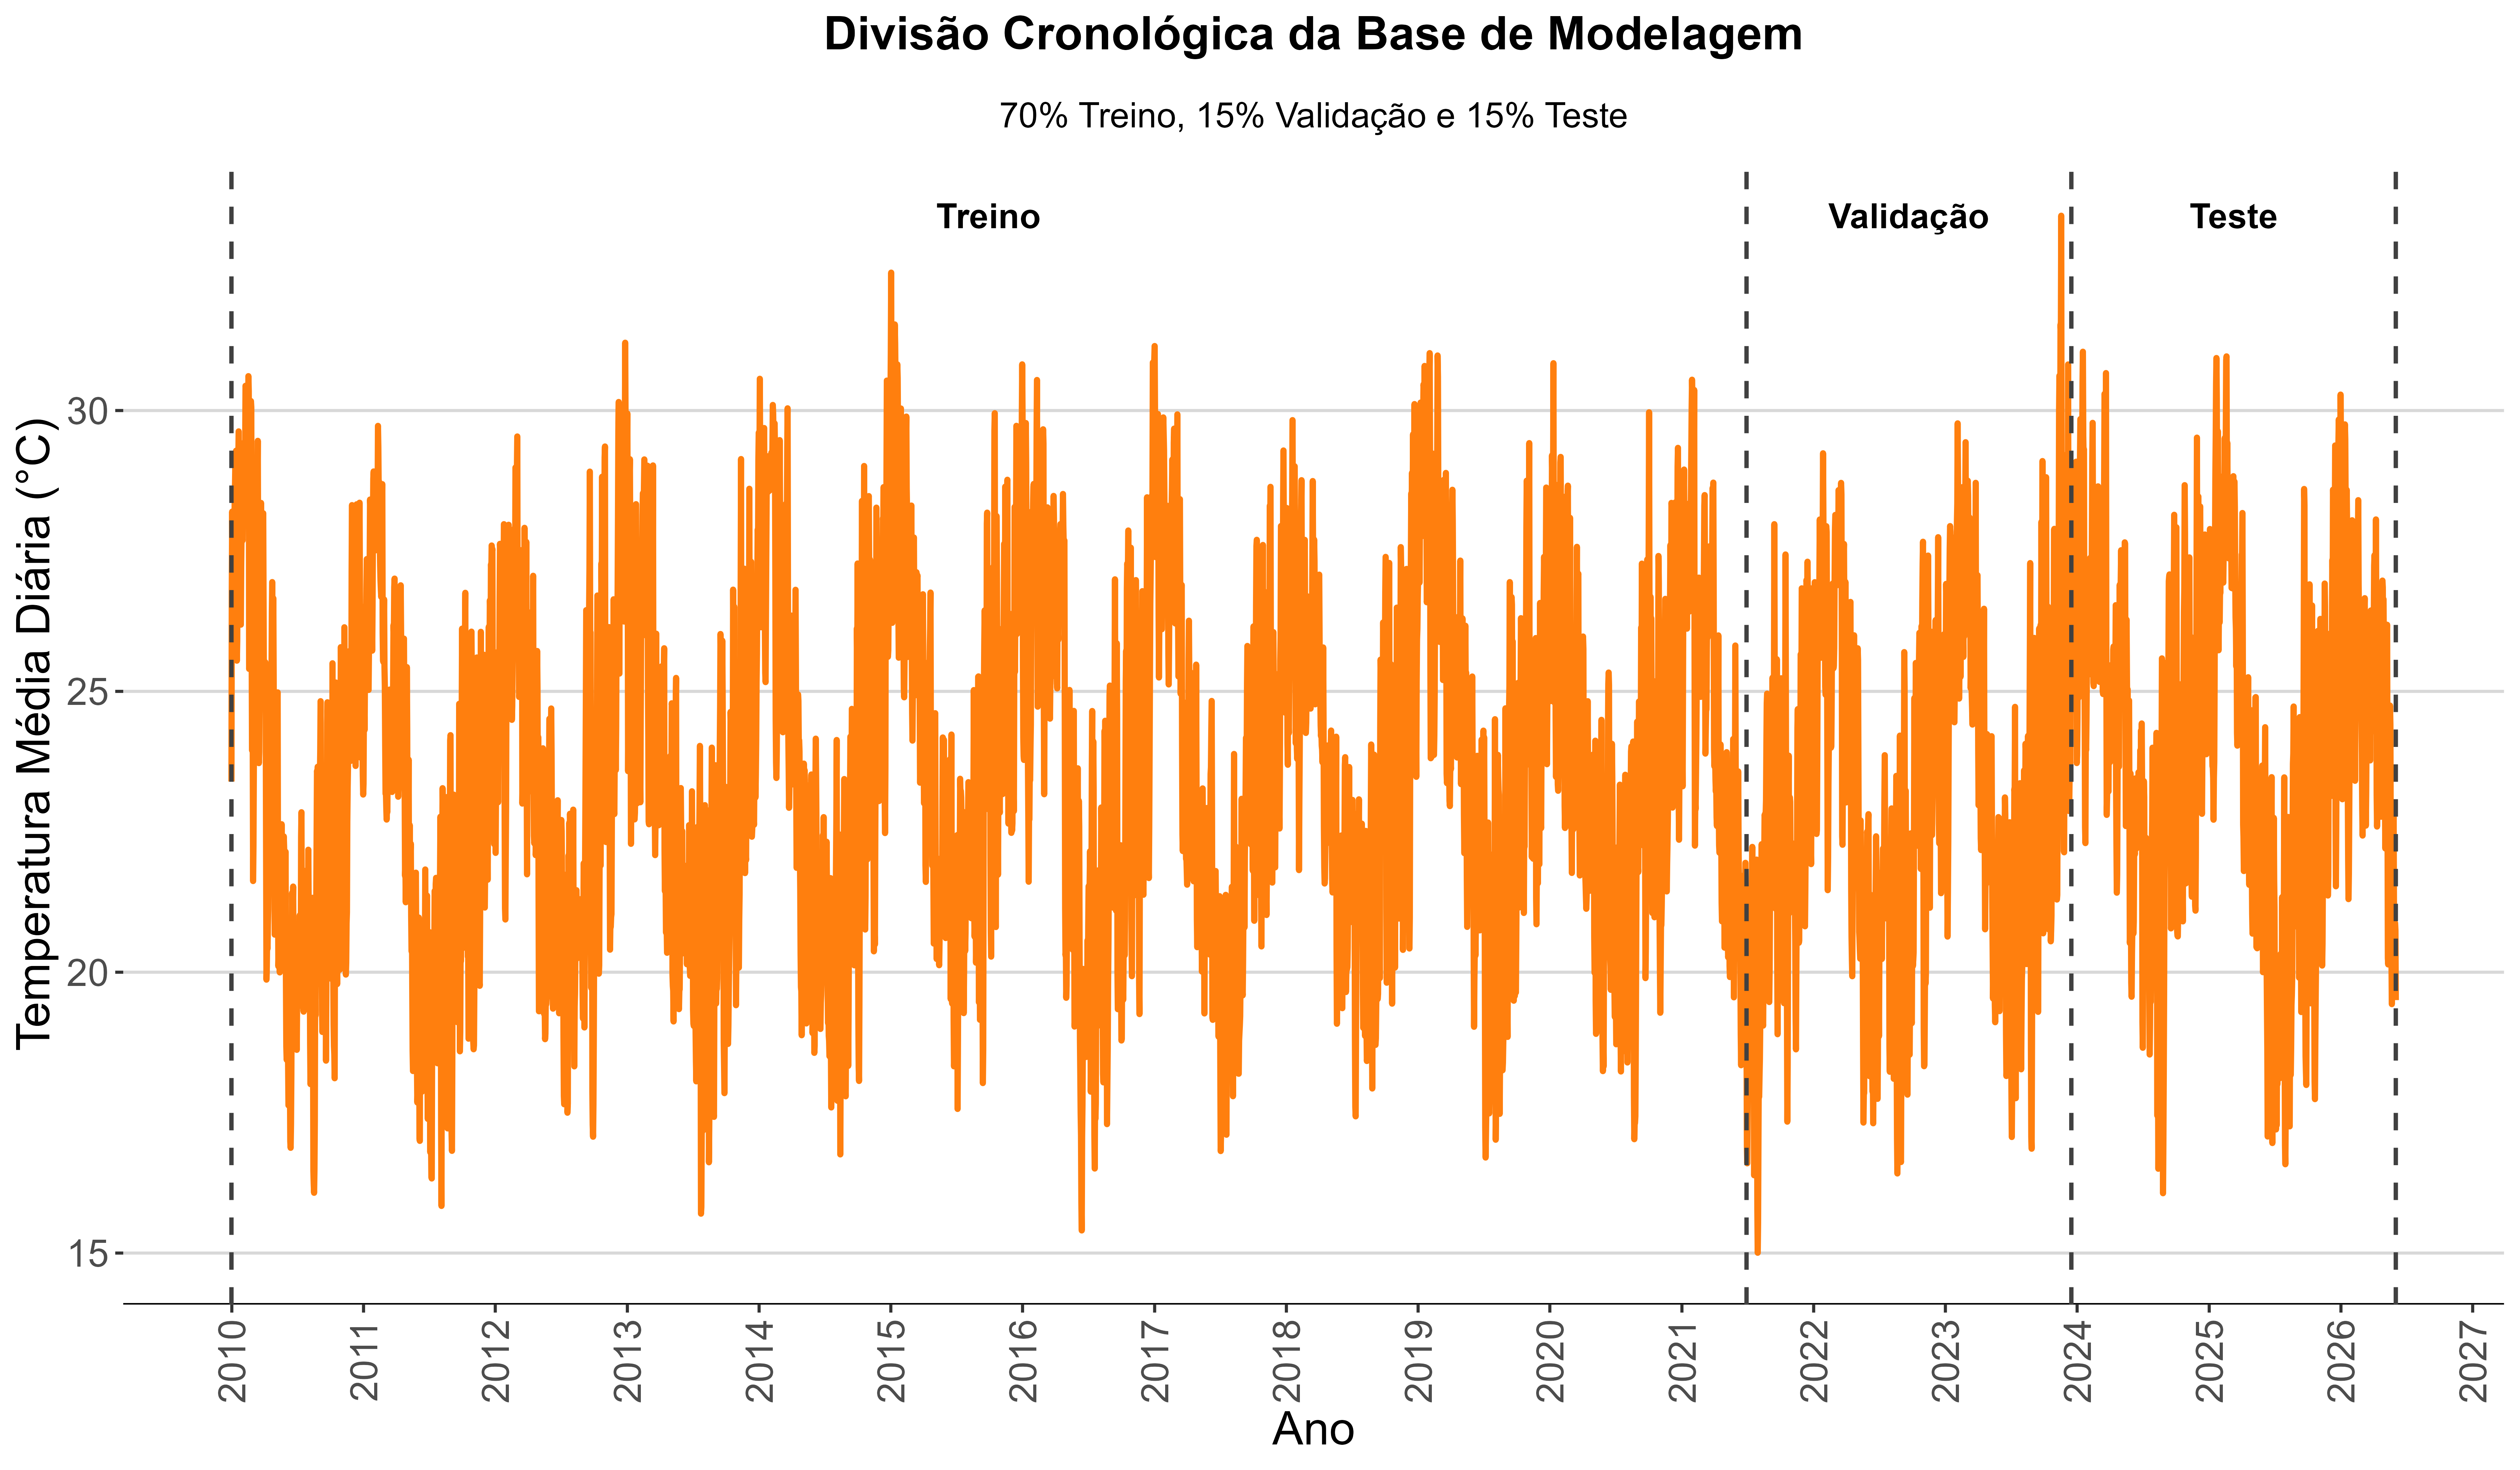
\includegraphics[keepaspectratio]{resultados/29_treino_teste_temperatura.png}}

}

\caption{Divisão Cronológica da Base de Modelagem}

\end{figure}%

A base foi dividida cronologicamente em três conjuntos:

{\def\LTcaptype{none} % do not increment counter
\begin{longtable}[]{@{}lcl@{}}
\toprule\noalign{}
Conjunto & Proporção & Início \\
\midrule\noalign{}
\endhead
\bottomrule\noalign{}
\endlastfoot
Treino & 70\% & 31/12/2009 \\
Validação & 15\% & 29/06/2021 \\
Teste & 15\% & 16/12/2023 \\
\end{longtable}
}

A divisão cronológica 70/15/15 preserva a ordem temporal e garante que o
modelo seja avaliado em um período não visto durante o treinamento. O
conjunto de teste (a partir de dezembro de 2023) cobre aproximadamente
dois anos e inclui ao menos um ciclo sazonal completo, o que é
suficiente para avaliar a capacidade de generalização do LSTM.

\section{Escolha dos
Hiperparâmetros}\label{escolha-dos-hiperparuxe2metros}

\subsection{Janela}\label{janela}

O hiperparâmetro \textbf{janela} define quantos passos de tempo
anteriores serão usados como entrada do modelo para prever o próximo
valor (ou os próximos \emph{k} valores).

\begin{figure}[H]

{\centering \pandocbounded{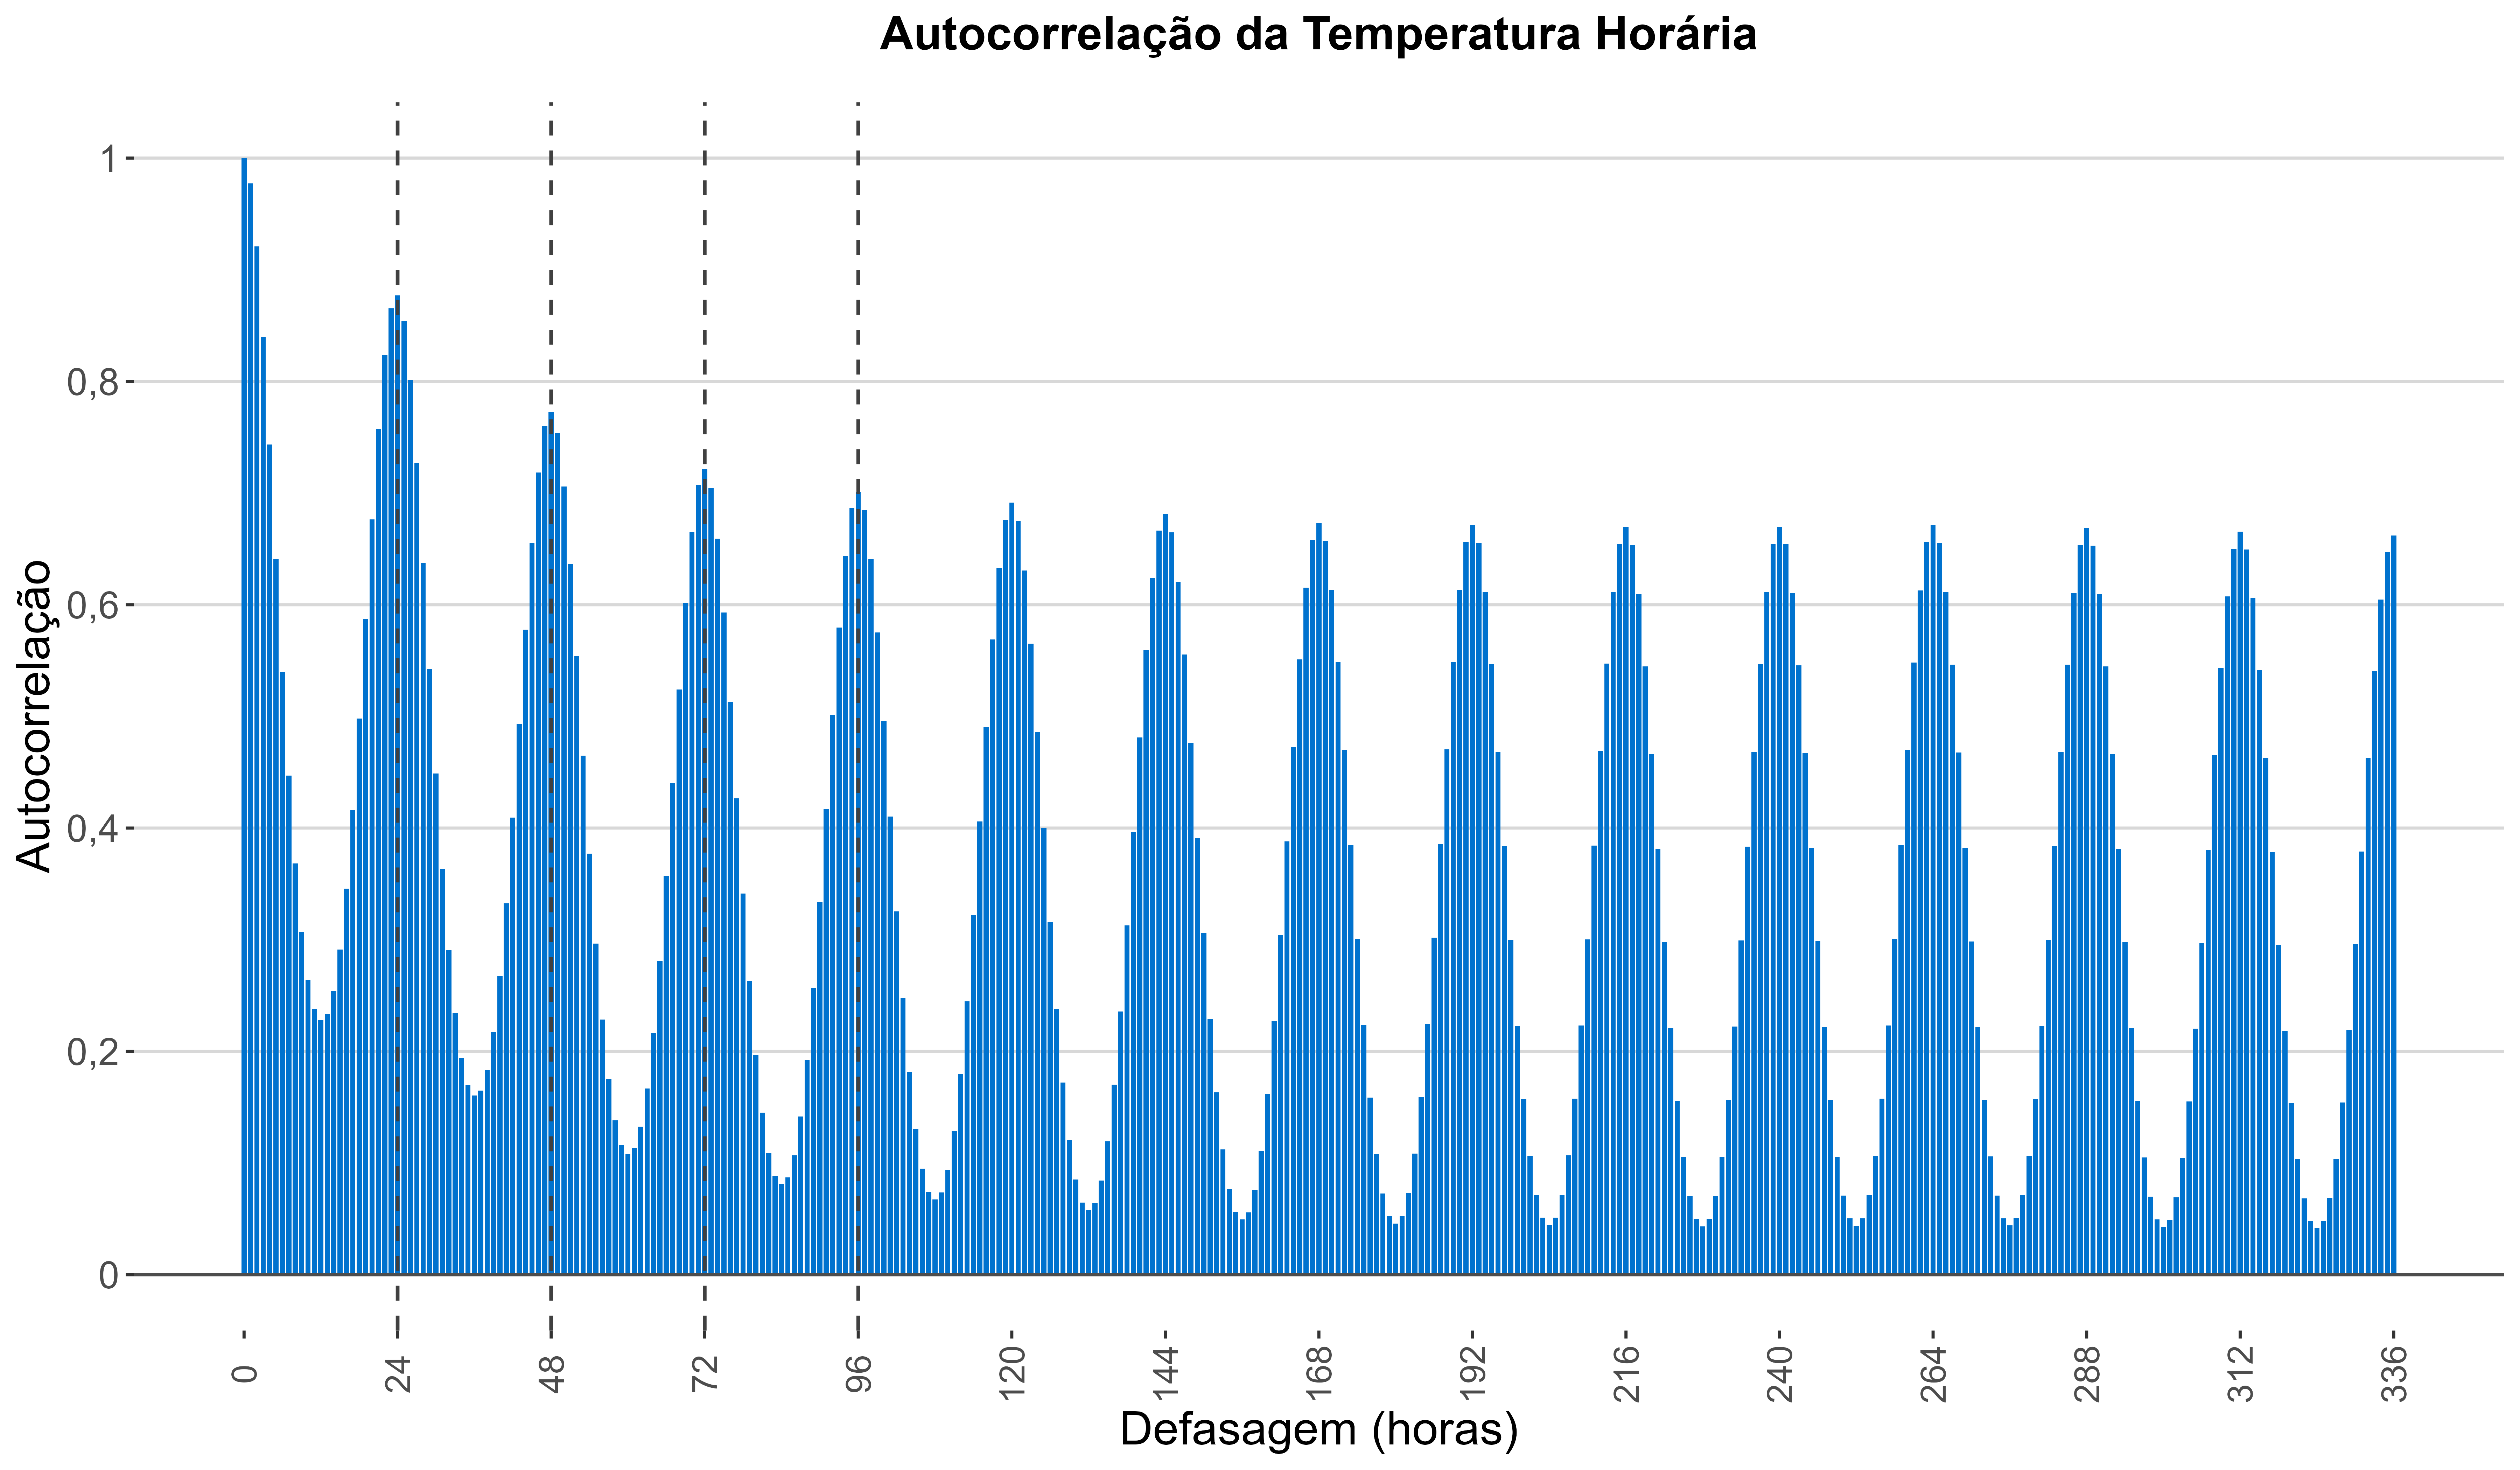
\includegraphics[keepaspectratio]{resultados/28_autocorrelacao_temperatura (muito importante).png}}

}

\caption{Autocorrelação da Temperatura Horária}

\end{figure}%

O gráfico de autocorrelação evidencia uma forte estrutura de dependência
temporal na série de temperatura horária, com correlações significativas
se estendendo por vários dias e picos pronunciados a cada 24 horas,
confirmando a sazonalidade diária. Com base nesses padrões, foram
escolhidas as seguintes janelas para comparação:

{\def\LTcaptype{none} % do not increment counter
\begin{longtable}[]{@{}cl@{}}
\toprule\noalign{}
Janela (h) & Justificativa \\
\midrule\noalign{}
\endhead
\bottomrule\noalign{}
\endlastfoot
24 & Captura um ciclo diário completo \\
48 & Captura o efeito de dois dias anteriores \\
72 & Captura o efeito de três dias anteriores \\
96 & Captura o efeito de quatro dias anteriores \\
\end{longtable}
}

\subsection{\texorpdfstring{Horizonte de Previsão
(\emph{k})}{Horizonte de Previsão (k)}}\label{horizonte-de-previsuxe3o-k}

O hiperparâmetro \textbf{k} define quantos passos à frente o modelo irá
prever simultaneamente. Foram considerados horizontes de até 24 horas,
cobrindo desde previsões de curto prazo até um ciclo diário completo:

{\def\LTcaptype{none} % do not increment counter
\begin{longtable}[]{@{}cl@{}}
\toprule\noalign{}
k (h) & Justificativa \\
\midrule\noalign{}
\endhead
\bottomrule\noalign{}
\endlastfoot
6 & Previsão de 6 horas à frente \\
12 & Previsão de 12 horas à frente \\
18 & Previsão de 18 horas à frente \\
24 & Previsão de 24 horas à frente \\
\end{longtable}
}

\section{Conclusão}\label{conclusuxe3o}

Esta análise descritiva dos dados ERA5-Land e Meteostat para Niterói,
RJ, cobriu as seguintes etapas:

\begin{enumerate}
\def\labelenumi{\arabic{enumi}.}
\item
  \textbf{Dados faltantes}: a base não apresentou nenhum dado faltante,
  resultado esperado dado o rigor do ERA5-Land como fonte de reanálise
  climática global.
\item
  \textbf{Análise univariada}: para cada uma das 13 variáveis
  meteorológicas foram geradas séries temporais nas escalas horária,
  diária, semanal e mensal, além de histograma e boxplot para
  caracterização distribucional.
\item
  \textbf{Análise multivariada}: séries sobrepostas por grupo temático
  (temperaturas, radiação, vento e pressão), matriz de correlação e
  gráficos de dispersão para identificar estruturas de co-variação entre
  as variáveis.
\item
  \textbf{Divisão cronológica}: a base foi particionada em treino,
  validação e teste, preservando a ordem temporal da série.
\item
  \textbf{Hiperparâmetros selecionados}:

  \begin{itemize}
  \tightlist
  \item
    \textbf{Janelas candidatas}: 24 h, 48 h, 72 h e 96 h --- escolhidas
    com base na autocorrelação horária da temperatura, que evidencia
    ciclos diários pronunciados e dependência de múltiplos dias.
  \item
    \textbf{Horizontes de previsão (k)}: 6 h, 12 h, 18 h e 24 h ---
    cobrindo desde previsões de curtíssimo prazo até um ciclo diário
    completo.
  \end{itemize}
\end{enumerate}




\end{document}
